%input macros (i.e. write your own macros file called MacroFile1.tex)
%\include{Macros/MacroFile1}

\documentclass[twoside,12pt]{Classes/myThesis}

\usepackage{amssymb,amsthm}
\usepackage{amsmath}
\usepackage{mathtools}
\usepackage{amscd}
\usepackage{mathrsfs}
\usepackage{accents}
\usepackage{listings}
\usepackage{graphicx}
\usepackage[all]{xy}
\usepackage{enumitem}
\usepackage{subcaption}
\usepackage{changepage}
\usepackage{xcolor}
\usepackage{bm}
\usepackage{xfrac}
\usepackage{booktabs}
\usepackage{multirow}
\usepackage{rotating}
\usepackage{listings}
\usepackage[labelfont=bf]{caption}
\usepackage[ruled,vlined,algochapter]{algorithm2e}
\usepackage{tikz}
\usepackage{microtype}
\usepackage{array} 

\usepackage[toc,page]{appendix}


%\newcommand{\ddt}[1][]{\frac{\textrm{d}#1}{\textrm{d}t}}
\newcommand{\Eqref}[1]{Eq.~\eqref{#1}}
\newcommand{\Figref}[1]{Figure~\ref{#1}}
\newcommand{\Tabref}[1]{Table~\ref{#1}}
\newcommand{\Chapref}[1]{Chapter~\ref{#1}}
\newcommand{\Secref}[1]{Section~\ref{#1}}
\newcommand{\Appref}[1]{Appendix~\ref{#1}}
\newcommand{\Algref}[1]{Algorithm~\ref{#1}}

\ifpdf
    \pdfinfo { /Title  (Stochastic branching and catastrophe with applications to intracellular pathogenics and the divergence of species )
               /Creator (TeX)
               /Producer (pdfTeX)
               /Author (Name Email)
               /CreationDate (D:)  %format D:YYYYMMDDhhmmss
               /ModDate (D:)
               /Subject (Thesis for the degree of Doctor of Philosophy)
               /Keywords (PhD, Thesis)}
    \pdfcatalog { /PageMode (/UseOutlines)
                  /OpenAction (fitbh)  }
\fi

%\title{\normalsize{Stochastic branching and catastrophe\\with applications to intracellular\\pathogenic replication and species divergence}}

\title{\large{
    Stochastic branching and catastrophe\\
    \vspace{1pt} % Adjust this to control the spacing between lines
    with applications to intracellular\\
    \vspace{1pt} % Adjust as needed
    pathogenic replication and species divergence
}}

\ifpdf
  \author{\href{mailto:email}{Adam Aldridge}}
  \crest{
\includegraphics[width=44mm]{Leeds_Crest.png}}
  \collegeordept{\href{http://eps.leeds.ac.uk/maths}{Department of Applied Mathematics}}
  \university{\href{http://www.leeds.ac.uk}{University of Leeds}}

\else
  \author{Name}
  \crest{
\includegraphics[width=54mm]{Leeds_Crest.eps}}
  \collegeordept{Department of Applied Mathematics}
  \university{University of Leeds}
\fi


\degree{Doctor of Philosophy}
\degreedate{November, 2024}

\hbadness=10000
\hfuzz=50pt
\usepackage{StyleFiles/watermark}




%%%%%%%%%%%%%%%%%%%%%%%%%%%%%%%%%%%%%%%%%%%%%%%%%%%






\usepackage{subcaption}    % for subfigures

\usepackage{amsmath}

\usepackage{enumitem}
\usepackage{float}


\usepackage{amsmath,amssymb}
\usepackage{tikz,pgfplots}
\usetikzlibrary{arrows, arrows.meta,shapes.misc, positioning, calc}


\usepackage{listings}
\usepackage{xcolor}



\usepackage[makeroom]{cancel}


\pgfplotsset{blankstyle/.style={%
    major tick length = 0,
    minor tick length = 0,
    tick label style={color=white},
    ylabel near ticks,
    ylabel style={rotate=-90,xshift=2mm},
    xlabel style={yshift=2mm},
    axis x line=bottom,
    axis y line=left}
}
\pgfplotsset{notblankstyle/.style={%
    minor tick length = 0,
    ylabel near ticks,
    ylabel style={rotate=-90,xshift=2mm},
    xlabel style={yshift=2mm},
    axis x line=bottom,
    axis y line=left}
}
\definecolor{airforceblue}{rgb}{0.36, 0.54, 0.66}

\newcommand{\pgf}{probability generating function}
\newcommand{\intinf}{\displaystyle\int_0^{\infty}}
%\newcommand{\pr}[1]{{\mathbb{P}\left(#1\right)}}

\newcommand{\pr}[1]{{\text{Pr}\left\{#1\right\}}}

\newcommand\mean[1]{{\rm I}\!{\rm E}(#1)}
\newcommand{\rr}{{\bf R}}
\newcommand{\xx}{{\bf X}}
\newcommand{\xt}{{\xx_t}}
\newcommand{\yy}{{\bf Y}}
\newcommand{\yt}{{\yy_t}}
\newcommand{\ww}{{\bf W}}
\newcommand{\wt}{{\ww_t}}

\newcommand{\xs}{{\xx_s}}
\newcommand{\vv}{{\bf V}}
\newcommand{\vt}{{\vv_t}}
\newcommand{\ddt}[1]{\displaystyle\frac{\dd #1}{\dd t}}
\newcommand{\dda}[2]{\displaystyle\frac{\dd #1}{\dd #2}}
\newcommand{\pddt}[1]{\displaystyle\frac{\partial #1}{\partial t}}
\newcommand{\pdd}[2]{\displaystyle\frac{\partial #1}{\partial #2}}
\newcommand{\dds}[1]{\displaystyle\frac{\dd #1}{\dd s}}
\newcommand{\dd}{{\rm d}}
\newcommand{\dt}{{\rm d}t}
\newcommand{\ee}{{\rm e}}
\newcommand{\ex}[1]{\mathbb{E}\left(#1\right)}
\newcommand{\de}{differential equation}
\newcommand{\rv}{random variable}
\newcommand{\delt}{\Delta t}
\newcommand{\ft}{\textit{F.~tularensis}}
\newcommand{\yp}{\textit{Y.~pestis}}

\newcommand{\Vt}{_{\text{total}} V}


\newcommand{\Ic}{ I_{\text{const}}}


\newcommand{\lb}{\left(}
\newcommand{\rb}{\right)}
\newcommand{\lrb}[1]{\lb#1\rb}

\newcommand{\lbs}{\left[}
\newcommand{\rbs}{\right]}
\newcommand{\lrbs}[1]{\lbs#1\rbs}

\newcommand{\xdt}{{\xx_{t+\delt}}}

\newcommand{\zz}{{\bf Z}}

\newcommand{\ydt}{{\yy_{t+\delt}}}

\newcommand{\pt}{p_{i,j}(t)}
\newcommand{\p}{p_{i,j}}	


\newcommand{\lbc}{\left\{ }
\newcommand{\rbc}{\right\} }
\newcommand{\lrbc}[1]{\lbc#1\rbc}

\newcommand{\lrbq}[1]{\hspace{-2pt}\lb#1\rb}

\newcommand{\Id}{{I_{\text{death}}}}
%\newcommand{\If}{{I_{\text{fix}}}}


\newcommand{\pdx}[2]{\displaystyle\frac{\partial #1}{\partial #2}}
\newcommand{\pdxn}[3]{\displaystyle\frac{\partial^{#3} #1}{\partial {#2}^{#3}}}


\newcommand{\eec}{{\ee^{\lambda(a-b)t}}}


\usepackage{amsthm} % for theorem environments

\theoremstyle{plain} % theorem style
\newtheorem{lemma}{Lemma} % define a new theorem environment called "lemma"


\usepackage{changepage} % for the adjustwidth environment








\begin{document}

\renewcommand\baselinestretch{1.2}
\baselineskip=18pt plus1pt

\frontmatter
\ifpdf
	\pdfbookmark[0]{Cover}{Cover}
\fi
\maketitle
%set the number of sectioning levels that get number and appear in the contents

\vfill
\noindent
To my knowledge, nothing has been plagiarised.  And despite it being remarkably helpful in coding,  none of the sentences presented were written with generative AI.   
\vfill

\pagebreak

\setcounter{secnumdepth}{2}
\setcounter{tocdepth}{2}


\ifpdf
	\pdfbookmark[0]{Copyright}{Copyright}
\fi
%\include{Copyright/copyright}
\ifpdf
	\pdfbookmark[0]{Publications}{Publications}
\fi
%\include{Publications/publications}
\ifpdf
	\pdfbookmark[0]{Acknowledgements}{Acknowledgement}
\fi
%\include{Acknowledgement/acknowledgement}
\noindent
\begin{center}
%Acknolagements 
\noindent
Thank you Grant, Martin, and Carmen,\\
\noindent
Each individually,  your knowledge and wisdom has shaped me much beyond understanding stochastic process theory. 

Especially Grant,  for always knowing how and when to encourage,  \\ and generally having the patience of a saint. 

Together, you have enriched the lives of countless aspirational students,  and I consider myself as greatly fortunate to have been one of them.\\

\vspace{29pt}
\noindent
Mum and Dad\\
\noindent
Thanks again for listening to me ramble on ad infinitum about everything and anything I happen to be interested in.  It's been invaluable in shaping my thoughts.\\


\vspace{29pt}
\noindent
Richard Teall, \\
For indulging my endless questions, being a patient and attentive guide,  and introducing me to some of the more arcane teachings of the yogavacara and the Gurdjieffiean framework.  Though I have to say you lost me a bit at the 18 trajectoris of the active,  passive and neutralising. 

\vspace{29pt}
\noindent

\noindent
I'd like to dedicate this thesis to all the wonderful people,  of the maths satalite office,  Buddhist meditation society,  of the caving club, and elsewhere,  who've been there along the way -- you know who you are.  Thank you for company,  guidance,  and companionship,  through ups and downs,  highs and lows,  for what can best be described as a mutually transformative series of events.



\end{center}


\vfill
\pagebreak

\ifpdf
	\pdfbookmark[0]{Abstract}{Abstract}
\fi


\begin{center}

\hspace{0pt}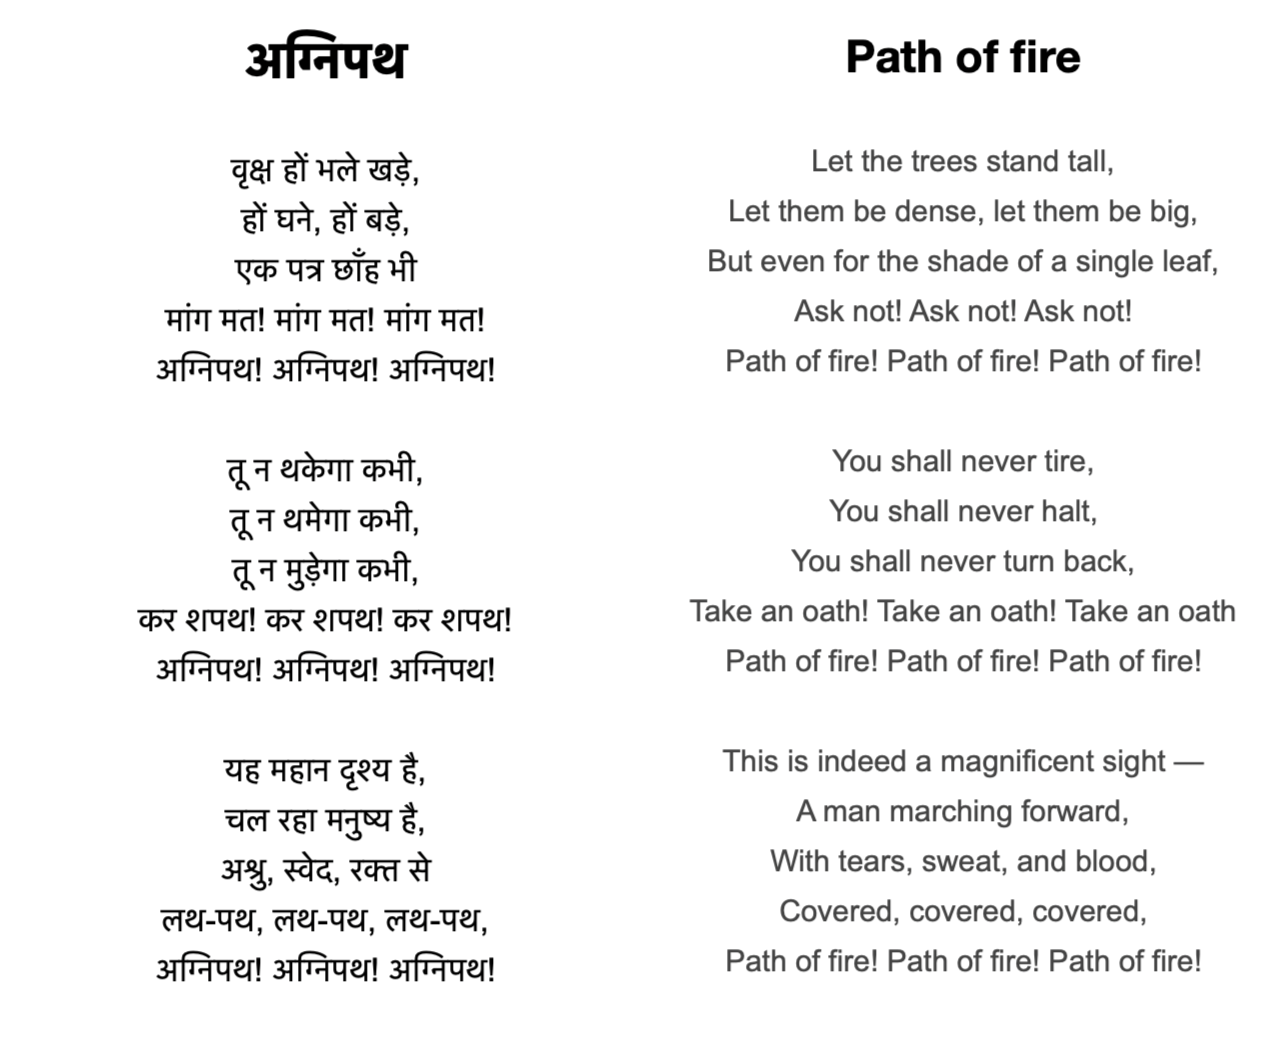
\includegraphics[width =0.74 \textwidth]{poemz.png}

A poem by Harivansh Rai Bachchan I've found interesting and have thought about a lot, especially in the final months, weeks and days of writing.\\


\vspace{12pt}
\noindent
Perhaps there is some implied causation from "not asking for shade" to the fact that the forest is thick and dense with trees. And in this regard,  there would be an analogy with the birth death catastrophe process: the propensity to "ask" aligning with catastrophe rate $\delta$, and large expected $\xt$ resulting from its diminishment -- the forest being dense and full of trees. \\

\vspace{12pt}
\noindent
When one pathway gets selected, the others in potential find themselves no-longer in the current basin of attraction. So without selection,  onward pathways can be numerous.  In the $\xt \to \infty$ limit, the draw from each diminishes to cessation.\\

\vspace{12pt}
\noindent
In a further (rather more dubious) potential analogy from here to the Vajrayana theory: the multifarious coloured lights of the bardo of dharmata \cite{trungpa2000tibetan} whizz and pop into a vast yet infinitely sub-divided tapestry,  without centre or circumference.  Leaving the journeyman undelivered,  thus unmarred, and increasingly without scope for reabsorption into the earthbound cycles of birth,  old age,  sickness and death. The essence of the teaching of the BT \cite{trungpa2000tibetan} seems,  as it were,  to "not ask" using means of being distracted by something else... 

\end{center}

\vfill

\pagebreak


\noindent
\textbf{Thesis abstract}

\vspace{0pt}
\noindent
The story of Yersinia pestis pathogenesis,  is largely elusive to detailed observation.  Not only is the bacteria sufficiently small to make direct observation challenging,  it is also potently deadly which brings heightened risks to experimentation. \par
This thesis,  however,  seeks to shed light on the evolved mechanisms of Y. pestis and other pathogens purely on the basis of theory.  It appears that the early stage dynamics of macrophage infiltration and intracellular replication could play a crucial role in the overall pathogenesis.  Serving as a means to facilitate the replication of those initial few colony forming units which enter the body,  the within macrophage environment may give Y. pestis the foot in the door it needs to bring greater probability to its continued proliferation in that body and onto the next.\par


Y. pestis,  has evolved to exploit the intracellular
environment of host macrophages for a temporary replicative advantage,  which, at the outset if its establishment in a host, may be crucial to its overall advantage.  As time progresses and the pathogen's 
presence becomes known to the body, more aggressive immune cells (neutrophils) are mounted and arrive on the scene of infection.
At this time, the same mechanism by which Y. pestis used to enter macrophages is turned off, thus protecting it
from these more hash leukocytes. From here it replicates extracellulary. 
The present thesis seeks to quantify the significance of this early replicative advantage. 



In addition, we have sought to understand the dynamics of lytic pathogenesis more generally, as opposed to 
constant budding release thought to be the mechanism of some viruses.
Much of the following mathematicical work surrounds the so called Birth Death Catastrophe process about which we have 
obtained a series of analytical results. \par

Then, also in the theme of early stage dynamics, I propose an inhomogeneous continuous time Markov chain model to descrive the emergence of species over a time characterised by population expansion into a yet unfulfilled domain, or through a period of upheaval following the triggering of an ecological instability. 

Through this, along with other models, I aimed to describe speculative theories of evolution.


The logistic speciation model is supplement to work presented by R. Mann in a paper exploring the statistical consequences of the standard birth death process as applied to large clade formation.  When conditioning on survival to the present, those lineages which did persist tend to have experienced a  period of greater than average diversification towards their outset.   This statistical consequence of the standard birth death process is refered to push of the past.  R. Mann and G. Budd propose that this is an overlooked dynamic in the paleontological literature,  which explores the reasons for observed mass origination events such as the Cambrian explosion, the great ordovician expansion, and the radiation and diversification of mammals following the cretaceous tertiary (KT) boundary. 
They don't dismiss the possibility that causes exist for these mass radiations, they merely comment that this demonstrateble statistical consequence has not yet been fully accounted for in the research.\par
The Logistic speciation model presented here seeks to face the problem from the other side,  serving as a means to immitate the dynamics by which an early mass diversification might be driven by the availability of resources during the early stages of a population expansion into a new area.\par
A topical example where such an event may have taken place is the evolution of Y. pestis from Y. pseudotuburculosis during the agricultural revolution \cite{king2009evolution} \cite{mira2006neolithic} where there would have been large populations amassing in villages offereing an abundance of replicative means giving the potential for bacterial genome variation. 




%\include{Abstract/abstract}
%\ifpdf
%	\pdfbookmark[0]{Abbreviations}{Abbreviations}
%\fi
%\include{Abbreviations/Abbreviations}


\ifpdf
	\pdfbookmark[0]{Table of contents}{TOClabel}
\fi
\tableofcontents


\mainmatter










\chapter{Introduction}










The Yersinia pestis bacterium is the causative agent of bubonic plague. Perhaps more than any other human pathogen, it has struck fear into the hearts and minds of peoples all over the world, and consciously or not lingers as a shadow in the western psyche. 

The present thesis will explore the mechanisms this bacteria employs in a human host, and the strategies it has evolved to overcome our innate immune system which possibly facilitated its historical success. 

We will paint a mathematical picture of an early stage plague infection with the aim of shedding light on the challenges faced by Yersinia pestis, and potentially the strategic advantege of its niche method.   




\subsection{Bubonic plague}
Yersinia pestis (Y. pestis) was first identified in 1890 by Alexander Yersin. It was later attributed (and only recently confirmed with genomic data) to have caused a number of major epidemics which killed a huge proportion of the European population and went on to shape the course of western cultural development. 


In 751AD there was Justinian's plague, but the most dramatic epidemic started in 1345 and may have killed as much as 50\% of the European population \cite{belich2022world}, with this figure reaching above 80\% in some urban centres. Successive waves of infection followed this and the continent didn't fully emerge from the plight until as late as the 17th century, with the 1666 fire of London often attributed as the watershed moment.\par
There were likely earlier Y. pestis epidemics reaching far back into history beyond the scope of accurate written account, perhaps recorded only in legend and myth. Evidence for this can be seen in a recent discovery that Y. pestis emerged from its evolutionary antecedent (Yersinia pseudotuberculosis) around 6000 years ago during what would have been a period of human population expansion driven by the development of agriculture. We may hypothesise that it was this excess supply of replicative means which provided the raw material for evolution. Facilitating a shift in phenotypes over the saddle into a new local optima. This representing the niche pathogenesis observed today in Y. pestis.



\subsection{Stochastic modelling}

Generally, at the outset of an infection, a relatively small number of colony forming units (bacteria or virus) will enter the body. 
Be it during inhalation into the respiratory system, through the skin with an insect's bite, or via ingestion, those initial pathogenic particles will be critical in determining the fate of the infection's success. 

The founding population will either be depleted to extinction, or expand to a capacity where its growth becomes established and requires a more targeted effort of the immune system to deal with. Whether they succeed in surviving beyond the first few hours of infection will depend on causes of a chance nature; encounters with cells and other immune factors that are subject to the randomness of Brownian motion.  


Stochastic effects play a more significant role in a population which is small. Because as the count of individuals increases, the dynamics of their overall growth and decline will become increasingly subject to the law of large numbers, and the expected fate of particular bacteria becomes telling of the group's trajectory. 

For this reason, because we are interested in the early stages of a Yersinia Pestis infection, it will be important to use stochastic models in our analysis.


\subsection{Branching}

Branching is one of the most fundamental patterns of behaviour observable in living systems. It is a basic means for the ordered structures of living entities to expand indefinitely in response to resource supply. Dividing one individual into two allows biomass and hence dissipative potential to increase without paying the cost required to increase agent complexity.\par

At the most basic level, replication of DNA molecules makes up the foundational component of all biological life. It is the maintenance and development of information, held up and carried forward against all odds of decay.\par

Understanding branching from a mathematical perspective has been a topic of probability theory since the end of the 19th century. Darwin's cousin, Francis Galton sought to understand the persistence of family names over generations. For this, with Henry Watson, he employed what would come to be known as the Galton Watson process  \cite{watson1875probability}. It's a discrete time stochastic process in which individuals either die or leave some number of offspring at each generation, fate being dictated by defined probabilities.\par 

It wasn't until the 1920s that continuous time models of branching were developed. In 1924, George Undy Yule published a paper in response to a book on evolution. The book was called ``Age and area'' and sought to understand the relationship between the number of species in a living genus and the area over which it spans. The paper  \cite{yule1925ii}, introduced what would become known as the Yule process. This was the first continuous time model of branching. Individuals only replicate, and do so with some probability during an interval of time:
$$\pr{\xx_{\Delta t + t}  = \xt + 1 \;\; | \;\; \xt} = \beta \xt \Delta t + o(\Delta t).$$
As the interval is taken in the limit, $\Delta t\to 0$, the probability that more than one replication takes place becomes infinitesimal. The fact that any of the $\xt$ present individuals can reproduce is encoded by the proportionality of the birth rate $\beta \xt$.\par This model, applied equally well to bacterial replication as to the emergence of species is also known as the standard birth process. Introducing death events, we get the standard birth-death process:

$$\pr{\xx_{\Delta t + t}  = \xt + 1 \;\; | \;\; \xt} = \beta \xt \Delta t + o(\Delta t)$$
$$\pr{\xx_{\Delta t + t}  = \xt - 1 \;\; | \;\; \xt} = \mu \xt \Delta t + o(\Delta t),$$

\noindent
which now has a universally accessible absorbing state at 0 representing extinction. Much of the work presented in this thesis surrounds our analysis of a further modification to this birth-death process. An additional ``catastrophe event'' is introduced whereby a sudden transition can take place from any non-zero count either to 0 or a separate ``rupture state'' (as per choice of definition).

$$\pr{\xx_{\Delta t + t}  = \xt + 1 \;\; | \;\; \xt} = \beta \xt \Delta t + o(\Delta t)$$
$$\pr{\xx_{\Delta t + t}  = \xt - 1 \;\; | \;\; \xt} = \mu \xt \Delta t + o(\Delta t)$$
$$\pr{\xx_{\Delta t + t}  = R \;\; | \;\; \xt} = \delta \xt \Delta t + o(\Delta t).$$

\noindent
In our case this is to represent the possibility of any resident bacteria within a white blood cell to trigger a bursting event in which the walls of the macrophage disintegrate and the pathogenic contents are simultaneously released. 





\subsection{Early phase Yersinia Pestis infection}

Y. pestis differs from its evolutionary antecedent, Y. pseudotuberculosis in a few ways but one stands out. Y. pestis exhibits two phases in its pathogenesis of mammalian hosts. In the first, the bacteria are readily absorbed by host leukocytes via phagocytosis (white blood cells, mainly macrophages and neutrophils). Within macrophages especially, the bacteria replicates in relative shelter and secrecy from patrolling immune agents.\par
In the second phase, after a switching period, they prevent this absorption by a combination of resistance and neutralisation. This is probably to avoid the more aggressive neutrophils which arrive at the infected area after a period, with recruitment following pathogen detection. This work explores the mathematical implications of this switching in an attempt to quantify the significance of the strategy's evolutionary advantage.\par 


This shift in phase of the incident bacteria occurs in response to sensing the warmer ambient temperature of a mammalian host. At a cooler temperature inside a flee, the bacteria remains in its first phase. Then after the flea bites its host, injected bacteria will after some delay shift behaviour to the second phase. The key difference acquired is resistance to phagocytosis. At the outset of invasion, colony forming units will be absorbed (phagocytosed) by host macrophages. With evolved resistance to their toxins, Y. pestis bacteria use this intracellular refuge as a temporary home to replicate and bolster numbers against challenges to come. The first mounted attack of the innate immune system is neutrophils. Summoned by various cytokines, they arrive on the scene in numbers, passing through the walls of blood vessels to the extracellular matrix in which the infection is beginning to take hold. After some time, an infected macrophage will rupture and its resident bacterial population will disperse into the extracellular matrix. Those Y. pestis bacteria which have undergone the transition to the second phase are characterised by being resistant to further phagocytosis.  Figure \ref{fig:two_columns_six_image} illustrates the dynamics. 





\begin{figure}[h!]
    \centering
    % First row of two images
    \begin{subfigure}{0.48\textwidth}
        \centering
        \includegraphics[width=\textwidth]{chapter1/YPwebsite/web1}
    \end{subfigure}
    \hspace{\fill}
    \begin{subfigure}{0.48\textwidth}
        \centering
        \includegraphics[width=\textwidth]{chapter1/YPwebsite/web2}
    \end{subfigure}

\caption*{Bacterial replication takes place within macrophage.  Some phase transitions occur.}
    \vspace{0.5em} % Small vertical space between rows

    % Second row of two images
    \begin{subfigure}{0.48\textwidth}
        \centering
        \includegraphics[width=\textwidth]{chapter1/YPwebsite/web3}
    \end{subfigure}
    \hspace{\fill}
    \begin{subfigure}{0.48\textwidth}
        \centering
        \includegraphics[width=\textwidth]{chapter1/YPwebsite/web4}
    \end{subfigure}

\caption*{Macrophage bursting,  more transitions to the second phase (red particles).  Neutrophils arrive.}
    \vspace{0.5em} % Small vertical space between rows

    % Third row of two images
    \begin{subfigure}{0.48\textwidth}
        \centering
        \includegraphics[width=\textwidth]{chapter1/YPwebsite/web5}
    \end{subfigure}
    \hspace{\fill}
    \begin{subfigure}{0.48\textwidth}
        \centering
        \includegraphics[width=\textwidth]{chapter1/YPwebsite/web6}
    \end{subfigure}

    % Single caption for all images
\caption*{Neutrophils phagocytose and eliminate remaining phase one leaving Y. pestis as a primarily extracellular infection.}
    \caption{A schematic representation.}
    \label{fig:two_columns_six_image}
\end{figure}







\subsection{HIV and the basic model of viral replication}
In the 1980s there was a major global HIV epidemic. This was terrible, killing around 40 million people over the decade, but it had the positive side effect of inducing a flurry of research into HIV pathogenesis and viral dynamics more generally. By the early 1990s progress was being made with the development of effective mathematical models describing within host viral replication.\par
Principal among these was what became known as the Basic Model of Viral Replication (BMVR) \cite{mclean1993balance}, which emerged from the fray of model diversity following the period of substantial experimentation. Its basic assumption was quite simple: there are three agent types

\begin{itemize}
\item \textbf{Susceptible cells: $S$} 

Host cells produced with a constant influx of rate $\lambda$, removed as they become infected by individual virions with a rate $\beta$.

\item \textbf{Free virions: $V$}

Produced at a constant rate, $p$, by each infected cell, and also cleared with rate $c$.

\item \textbf{Infected cells: $I$}

A single free virion coming into contact with a susceptible cell is sufficient to convert it into an infected cell. Naturally, this uses up the virion and removes one succeptible cell from $S$. Infected cells then produce new free virions at a constant rate, not accounting for the likely reality that a higher intracellular load might cause a cell to be more productive. Though some models do include a lag period between the time a cell is infected and when it begins to produce virions.\par
They are also removed by cell death with rate $\delta$.
\end{itemize}

\noindent
The equations are as follows

\begin{align*}
\ddt{S} & = \lambda - \beta SI\\
\ddt{I} & = \beta SI - \delta I\\
\ddt{V}& = p I - c V.
\end{align*}

\noindent
In some cases, the model is simplified by taking the number of susceptible cells as a constant, $T$. This represents the situation in which there is a large availability of cells to infect such that their depletion is not a significant driver of the overall dynamics. With this simplifying assumption, the equations become,

\begin{align*}
\ddt{I} & = \beta TI - \delta I\\
\ddt{V}& = p I - c V.
\end{align*}

\noindent
To be clear, this rests on the assumption that virions are produced by cells one by one at a constant release rate.


\subsubsection*{New research into HIV viral release}

In 2018, an experiment was done at Los Alamos \cite{hataye2019principles} with the intention of quantifying the release dynamics of HIV virions from infected cells. A tray of 32 small ``wells'' were each filled with some liquid each containing exactly one cell infected by HIV. Then over a period of days, viral counts were measured from the liquid of every well at intervals of one hour.\par

If the assumption of the BMVR were correct, we would expect to see something approximating a Poisson process in each well, with roughly the same count recorded in all of the wells at each interval. What was actually observed was very different: huge variation between wells, and the production rates were not at all constant. Instead, a high degree of intermittency was recorded. Cells remaining completely inactive for successive intervals, then occasionally releasing a substantial number of virions, seemingly all at once. \par

Clearly, this challenges the standard assumption of constant-rate budding. It also raises a speculative question: Could this commonly held belief about viral release have been to some extent patronised by widespread use of the modelling assumption? We'll probably never know, but it's curious to consider.\par

\subsubsection*{So what?}
In any case, the observation is interesting and it begs the question: why? There will be some reason HIV has evolved to use this quasi-bursting procedure. Perhaps it is simply more convenient for release to take place in floods. Passage through the cell wall requires an opening, and it surely makes sense to only induce this periodically; avoiding both unwanted leakage of cellular components and ingress of extracellular debris.\par 

But perhaps there is also some general advantage to be gained by virions being released in large cohorts like this. It could be that locally deletable immune factors are flooded and overcome by the sudden outflux of enemy agents. A paper by N. Komavora \cite{komarova2007viral} presented this idea of a so called ``flooding'' advantage. She used the analogy of a criminal gang trying to escape their trap house which is surrounded by police: ``If we all run out at once, maybe some of us will get away in the confusion''.\par 

Analysis of pathogen release strategies and their potential makes up the topic of chapter 6, with attention paid to the spectrum between budding release, and complete cell bursting.\par

Back on the topic of the BMVR and its potentially flawed assumption, in chapter 4 we propose a possible modification to the viral release term, $pI$, in an attempt to account for intracellular dynamics consistent with the birth death catastrophe process. 












\subsection{Pathogenic release strategies.} 

With both viral and bacterial particles being very small, it has historically been extremely challenging to make good observations of their behaviour. Progress is taking place, and in the last couple of decades, we have been able to observe individual bacteria through the course of an intracellular infection. For example, Dstl (Defence science technology laboratory) has been able to record videos of a macrophage bursting to release on the order of 100 Francisella Tularensis bacteria. Through the induction of bacterial luminescence, each individual pathogenic particle can be visually isolated and counted.\par
Francisella Tularensis and Y. Pestis are similar in size, each around 0.5 micrometers (Y. pestis being marginally larger). But viruses are generally about an order of magnitude smaller than bacteria, with HIV being approximately 100 nanometres. They are hence somewhat more elusive to visualisation and counting.\par 



\subsubsection*{Bursting}
Both Francisella Tularensis and Yersinia Pestis multiply within macrophages becfore causing the cell to lyse, releasing their pathogenic cohort for further replicative endevours. The case of Y. Pestis is slightly more complicated with a biphsaic switching; a change from intracellular to extracellular replication (more on that later). But generally, these strategies which involve a complete release in combination with the death of the cell are reffered to as bursting pathogenesis.

\subsubsection*{Budding}

As described above, budding release refers to the situation where an infected cell outputs new virions at a constant rate. Models of viral replication generally take this as an assumption and it has become a commonly held belief that this is how viral release takes place. 


\subsubsection*{Something in between?}

The recent work experimenting HIV release reveals that the story may not be so simple as was previously assumed. That in cases of non-lytic virulence there may be various strategies we are not fully aware of. Another example of something in between bursting and budding is release by extracellular vesicles (EVs). Amongst viruses that leave the cell non-lytically, there is a subdivision to be made into those which produce and assemble their own protein shell to harbour genetic material, and those which exploit the cell membrane to produce a lipid container. Of this second group, it has been known for a while that in some cases, multiple individual viruses get contained and released in one ex-membrane capsule. These are reffered to as extracellular vessicles \cite{kerviel2021new}, \cite{buzas2023roles}. They present another potential coplexity to the story of viral release.









\subsection{Research questions}

There are four key areas of focus that this research seeks to address. The first two are questions into the nature of biological process:

\begin{itemize}
\item  \textbf{Why did Y. pestis evolve a biphasic pathogenesis in humans?} 
Switching from pro-phagocytosis to an antiphagocytosis strategy seems to be crucial to the overall pathogenesis of Y. Pestis.  There is a simple argument based on the net proliferability both before and after neutrophils arrive on the scene of infection (see conclusion).  Also,  we could assume that Y. pestis replication is only slightly supercritical.  And it can be easily demonstrated that near critical branching process become drastically less likely to die out when the initial count is increased by even a few colony forming units.  If we see the initial within macrophage replication as setting up an initial population,  this effect offers further explanatory potential. 



\item \textbf{Is there a general advantage to "bursting" style transfer in successive intracellular infection methods?}
Natalie Komavora proposed that there could be a "flooding advantage" to bursting style pathogenesis.  That is,  bacteria or virus exiting their host infected cells all at once in large groups rather than one at a time or in dribs and drabs. Chapter 7 explores gives further mathematical support to this theory and discuses the conditions under which it might prove effective.
\end{itemize} 

\noindent
The second two are areas in which we tried to construct new models to describe particular dynamics:

\begin{itemize}
\item \textbf{A potential update to the standard BMVR model of viral replication to incorporate intracellular dynamics.}
Based on our analysis of the birth death catastrophe process, there is the possibility that one of the results could be encorporated into a rate of the BMVR.

\item \textbf{Efforts to describe variable rates of evolution with Markov chains}\par
The standard birth-death process has been used for decades to model the emergence of species over geological time periods. It may however be criticised for being consistent with the outdated doctrine of progressive gradualism. This states that evolutionary change is constant and happens gradually. In the 1970s,  S. J Gould proposed the counter theory of punctuated equilibria: evolution taking place rapidly over proportionally short periods which are intervened by longer times of relative morphological stasis.\par
There is also the controversial question of why large clades (containing many species) appear to generally have experienced an initial period of substantial diversification. Some attribute this observation to a statistical consequence of standard birth-death dynamics (push of the past, and pull of the present).\par
This work presents two models which seek to challenge this argument, and give mathematical basis to the punctuated equalibria theoretical paradigm. Notably, there is potential significance here in understanding the emergence of Y. Pestis.


\end{itemize}











\subsection{How the content is divided amongst the chapters}

Broadly, the thesis can be divided into three main parts: Introductions,  analytical results in relation to the Birth Death Catastrophe process,  and models of resulting from my curiosity.  Including this introduction and the conclusion,  these parts are divided amongst 8 chapters.  Below is a summary of the content and message of each.












\subsubsection{Chapter 2: Mathematical context}




Much of the work presented in this thesis surrounds topics of stochastic process theory,  and specifically branching processes.  Both continuous time and discrete time branching processes are examples of Markov chains exhibiting the Markov property: The probability of what happens next depends only on the current state of the system,   not on any past events;
\[
P(\xx_{t+1} = x_{t+1} \mid \xx_t = x_t, \xx_{t-1} = x_{t-1}, \ldots, \xx_0 = x_0) = P(\xx_{t+1} = x_{t+1} \mid \xx_t = x_t).
\] 
Continuous and discrete time Markov chains differ in their methods of analysis.  For example,  the fixation probabilities of discrete time processes can be understood using first step analysis which considers the single-step possible moves and their probabilities.  Continuous time chains on the other hand can be dealt with using the forward Kolmogorov Equation.  It is worth noting that continuous time chains can be "embedded" into discrete time versions by considering the probability distribution of \textit{next} events.  But when it comes to branching processes,  this fact shouldn't give the false impression that the two types of process are somehow identical in their dynamics,  just on modified time axes. Discrete time branching proceses differs fundamentally in that every individual either replicates or dies at once in each time step.  In the continuous time birth death process,  only single jumps up or down are possible at each move.  And this difference means there isn't a clear analyitical transformation between the two types of model.\par
It should be noted that we will only be dealing with discrete state space processes (jump chains).  Continuous state space models are also of interest, but the application to cellular replication nautrally lends itself to models with countable units. 
\vspace{10pt}

\noindent
One of the most important aspects of branching processes is their net replacement. This has slightly different interpretations in discrete and continuous time branching but esentially means the same thing.  It is the rate of change of the expected process count.  In discrete time: the expected number of offspring produced by a single individual in its lifetime.  
$$\mean{Z} = 2 p + 0(1-p) = 2p$$  
where p is the probability of an individual to replicate rather than die (wp $1-p$), and $Z$ is the number of offspring left by the one individual. \par 
In continuous time,  rate of population expansion,
$$\ddt{\mean{\xt}} = (\beta - \mu) \mean{\xt},$$
is quantified by $\beta - \mu$,  the net replication rate. 
In each case,  whether this number ($2p$ or $\beta - \mu$) is larger or less than 1 is of great signigicance. 




\begin{itemize}
\item When $2p$ or $\beta - \mu$ greater than 1,  the process is caled supercritical.  (see figure 1.2)
\begin{figure}[h!]
\centering
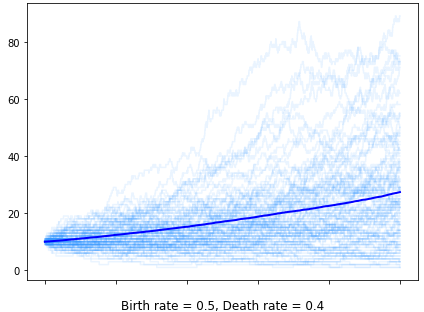
\includegraphics[width = 0.55\textwidth]{chapter1/imgs/BD54}
\caption{Supercritical birth death in continuous time.  In this and the following two figures, a large numer of individual realisations are shown in light blue, and their average is drawn in dark blue.  In each case, the sample mean shown forms a good approximation of the analytical mean.}
\label{im1}
\end{figure}
Some realisations die out, the rest continue rising towards infinity in an increasingly redictable exponential fashion. 
\end{itemize}




\begin{itemize}
\item When $2p$ or $\beta - \mu$ less than 1,  subcritical.  
\begin{figure}[h!]
\centering
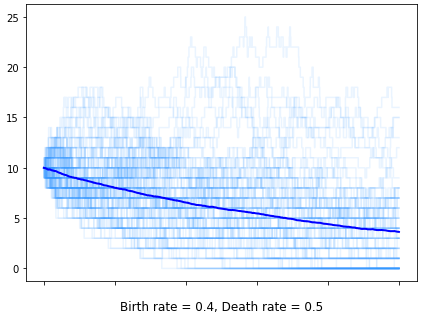
\includegraphics[width = 0.55\textwidth]{chapter1/imgs/BD45}
\caption*{Subcritical}
\end{figure}

All subcritical realisations are destined to die,  fixating at 0.


\end{itemize}



\begin{itemize}

\item And when $2p$ or $\beta - \mu$ is equal to 1,  the process is reffered to as critical.   

\begin{figure}[h!]
\centering
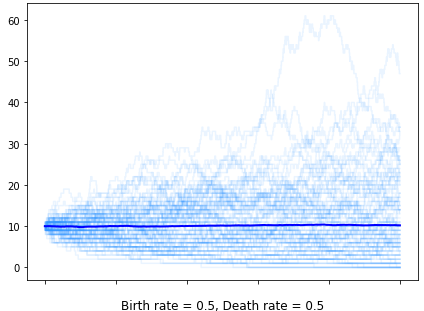
\includegraphics[width = 0.55\textwidth]{chapter1/imgs/BDpoint55}
\caption*{Critical}
\end{figure}

Line in the subcritical case, all critical realisations are destined to die out, but curiously, the expect time in which then do this is infinite.  A single process could possibly last for a very long time,  never fixating. 

\end{itemize}






































\subsubsection{Chapter 3: Birth death catastrophe model -- main results}

This chapter introduces the Birth Death Catastrophe (BDC) process and outlines a series of results asociated with in. \par


\noindent
Around the 1980s, work was being done into growth models that incorporated stochastic declines (shocks). Out
of this came the the birth death catastrophe model as we know it \cite{cairns2004extinction}\cite{brockwell1985extinction} \cite{brockwell1982birth} \cite{dori2018family}.  An extension of the standard birth death
process, but where from every state apart from 0, a catastrophe event can take place, either causing a transition
to 0, or a special catastrophe state. Similar to birth and death events, this catastrophe state can be initiated by
any of the individual units, and so occurs with a rate proportional to the population size. We were interested
in this model for its potential application in modelling the development of an infection within cells that burst.
And more broadly, infections that spread amongst multiple cells.
Here the BDC model is defined and some key equations are introduced which describe the mean and variances
of the process. Some of the results have been found by others before, but we also have a few which extend beyond
the current literature. For example, we have a formula for the second moment of the process count in terms of the non-rupture probability. This, along with the process variance we found by solving a series of four ordinary differential equations.\par

Some attention is given to limiting conditional distributions. That is the behaviour of the process count assuming that by some late time fixation has not yet occurred.  We show that in some cases, quasi-stationarity is exhibited and we quantify the quasi-stationary mean as a function of rate parameters for replication and rupture.






\subsubsection{Chapter 4: Birth death catastrophe model -- additonal results}

This chapter extends the pervios one with more results,  especially those associated with state probabilities which are obtained from the forward Kolmogorov equation with the method of characteristics. 




\subsubsection{Chapter 5: Birth death catastrophe process -- modifications}

Here we explore the analytical possibilities of two modified BDC processes
\begin{itemize}
\item $\mathbf{N = 2}$ \textbf{sucessive imediate transfer}. We were generally interested in producing some kind of model which captured the dynamics of between-cell transfer and growth.  Moving in this direction,  we spent some time developing results in relation to the successive BDC process whereby a second process begins at the rupture of the first.  The anaysis didn't lead to exactly what we were looking for, but we found some distributions along the way,  and the work ultimately went on to lay the groundwork for the "fixed removal" model of chapter 6.   


\item \textbf{Two type}.  In 2011,  Antal and Krapivsky \cite{antal2011exact} published an exact solution to the two type continuouts time birth death process with one way mutation.  We were able to use their particular method, with some changes of variables,  to obtain the equivalent result for the two type BDC process.  This section simply outlines the process by which the result can be found. 


\end{itemize}


\subsubsection{Chapter 6: Bursting-budding comparrison}



Work has been done by others \cite{komarova2007viral} \cite{yuan2011stochastic} \cite{pearson2011stochastic} \cite{capistran2018extracellular} comparing the fundamental dynamical differences between budding and bursting style pathogenesis.  N. Komavora, for example proposed a potential advantage to busrting due to a flooding effect.  This chapter explores the significance of release counts when considering successive infiltration models.  That is, where pathogens go from one infected cell to another. \par
Each of the parts of this chapter consider he importance of locally depletable immune factors.  With only a finite supply of chalenges,  there is a sort of saftey in numbers effect.


\noindent
\textbf{Replicator suppressor}
This part considers the intracelllular environment in which there are toxin containing granules such as there are in macrophages and neutrophils.  Similar to a predetor pery model,  there are two individual types: replicators (pahogenic particles) and suppressors (granules).  It is clearly demonstratable that a larger incident population of replicators will have disproportonatly beter odds of survival and persistence in this case as more bacteria will be available to deplete the present immuno reserves. 



\noindent
\textbf{Fixed removal}
Moving from the intracellular to the extracellular environment. This part considers the question of how many released pathogenic particles manage to reach their next host.  In the extracellular medium between host cells there are a number of immune chalenges that the pathogens have to face. \par
For example,  complement proteins, which puncture bacterial cells deemed to be invaders,  and host bacteriophages which are viruses living in simbiosis with the organisms that may serve to kill forein agents. \par
The assumption is that these immune factors are locally depletable and that a larger group release of pathogens will somehow cause a flooding effect analogous to the one proposed by N. Komavora. 








\subsubsection{Chapter 7: Variability in evolution}
No topic has seduced and captivated my curiosity more than the question of what life is,  how it evolves,  and whether we can determine general underlying dynamics which uncover aspects fundamental to the reality of rise,  change,  and decay of living agencies. \par

Evolution into species, harbours a yet unsolved mystery to science.  We do know a lot.  For example,  vast efforts have been made in the last 5 decades into uncovering the microbiological mechanisms which underpin the replication and usage of DNA. \par


With regards to a big picture view,  progress is being made \cite{sharma2023assembly},  but we are yet to produce a widely taught and accepted description of what life is and how it changes which is consistent with concepts of neg-entropy production and thermodynamics more generally at the micro and macro scales. \par

But the hum and the buzz has been around for a while now,  and perhaps the writing is even on the wall as to how a water-tight conception might unfold.

Unfortunately,  this thesis does not have the answer.  Not only am I considerably under-qualified for the task,  but this project was supposed to be about Yersinia Pestis,  and it largely is.  Of course,  Y.  pestis bacteria is one of the most acute examples of a living dissipative structure.  \par

\vspace{10pt} 



\noindent
 Mostly before the PhD and in the first year,  I read a few books which went on to change the way I thought about science,  philosophy,  and particularly the topic of evolution.  Most significantly: 



\begin{itemize}
\item \textbf{Order out of chaos,  Mans new dialogue with nature --  Ilya Prigogine and Isabelle Stengers,  1984}
Outlines the theory of dissipative structures -- chaotic order formations which take place as local reductions in entropy in the as a means of dissipation in the context of a wider increase in entropy consistent with the second law \cite{prigogine2018order}.

\item \textbf{What is life -- Erwin Schrödinger, 1944}
Frames the problem of understanding what life is in the context of energy gradients,  neg-entropy and the laws of thermodynamics \cite{schrodinger1946life}.   

\item \textbf{Chance and necessity -- Jacques Monod, 1970}
Overviews the (at the time) new understanding of DNA molecular biology and mechanisms of replication and transcription \cite{monod1974chance}.  Then explores the concept of teleology and what it means for living objects, made of mere chemistry, to have volition. \par 
Outlines animism and vitalistic schools of thought and belief.

\item \textbf{The genetical theory of natural selection -- Ronald Fisher, 1930}
Covers the topic of evolution broardly from a mathematical perspective. Then goes on to discuss the implications of birth rates being different among sectors of society.  Also the rise and fall of civilisations. \cite{fisher1929genetical}. 

\item \textbf{Wonderful life -- Stephen J Gould, 1990}
All about the Cambrian explosion,  a geologically instantaneous period of a few million years in which great diversification of species took place.  Contrasting the previous Ediaceran fauna of docile wandering discs of the sea floor, all of a suden, there were a vast array of segmented athropodic forms.  Displaying arms, legs, eyes, mouths and claws;  eating one another and josstling for survival in what must have been a tropical tempo of savage egoisms \cite{gould1989wonderful}. 

\item \textbf{Beyond good and evil -- Friedrich Nietzsche}
Covers a wide range of topics surrounding, from the historical development of moralities to the emergence of species in relation to environmental conditions and suspended potential within a population.  \cite{nietzsche2013beyond}

\item \textbf{(Some of) On the origin of species -- Charled Darwin, 1859}
Needs no introduction.  Hard to read though with the old timey langauge style! Mostly interested in what he said of rate of variation in cases of domesticated animals.  \cite{darwin1859origin} 
\end{itemize}



They drew my attention to fact that the rate of evolution and divergence into species,  among other things,  is driven by a combination of selective pressures and energy availability.  For example,  the presence of competing species and how much food is readily available for a given population in its ecosystem.  It seems that these two factors make up a kind of push-pull tension,  simultaneously holding a group together with the necessity to conform so as to be strong in the face of competition for survival; whilst constantly pulling it apart with the ravenous impulse of variation which is a natural component of living matter as consistent with the second law of entropy increase. \par

Nietzsche writes about this sort of dynamic in ``Beyond good and evil" section 262:

\begin{quotation}
\noindent
"A species arises, a type becomes fixed and strong through protracted struggle against essentially constant unfavourable conditions. Conversely, one knows from the experience of breeders that species which receive plentiful nourishment and an excess of care and protection soon tend very strongly produce variation of their type and are rich in marvels and monstrosities"
\end{quotation}

\noindent
Sexual selection also offers a mystery in this space.  It seems to both macroscopically bring a population together through mixing of traits whilst also (microscopically) introducing disorder into genomes crossed over.  I won't attempt to make heads or tails of this apparently confusing juxtaposition.  Maybe someone else has and perhaps it isn't as confusing as it may appear. \par 

\vspace{10pt}

\noindent
 
\noindent
But my suspicion is that there is a underlying dynamic to articulate.  That there is a building of tension,  and release at the advent of more favourable circumstances.  And that this takes place in a cyclic fashion across multiple domains. \par

That this release is as it were more dissipative,  and during it,  when there is a greater fanning out of forms,  that this is an example of a dissipative structure which produces a chaotic formation of complex order in the form of bifurcating species and forms.  Sort of as in fluid turbulence bifurcating fluid trajectories create a chaotic dissipation of heat through friction.  The analogy is albeit more artistic than scientific,  but fun to think about! \par
If we consider the example of planar flow around a circle,  there is here this property of a cyclic to and fro -- flow speeding up followed by turbulence shedding,  low pressure and repetition. 

\vspace{8pt}
\hrule 
\vspace{8pt}
\noindent
\textbf{Bit of an aside:} I can't help but be interested in the possibility that this sort of speculated dynamic could be used to apocryphally explain cultural trends in societies.  One potential example is the apparent trend for strict conservative values to become prevalent after a period of substantial economic and cultural dynamism which ultimately brought about liberal tolerance.\par

It could be hypothesised that this has happened at least twice before in history: In Iraq and the middle east more broadly after its golden age of expansion in the first few centuries of the second millennium, and also in Sumatra and Java of Indonesia in the 16th century after the eventual decline of the Hindu kingdoms.  (The Hindu court culture was all pushed to Bali where it survived -- see David Attenborough's 1969 documentary "The miracle of Bali",  It's not particularly relevant to the point,  but definitely worth a watch anyway).  Note: I only discovered the theorey of anacyclosis \cite{podes1991polybius} after writing this, but there appears to be some similarity. 

\begin{figure}[h!]
\centering
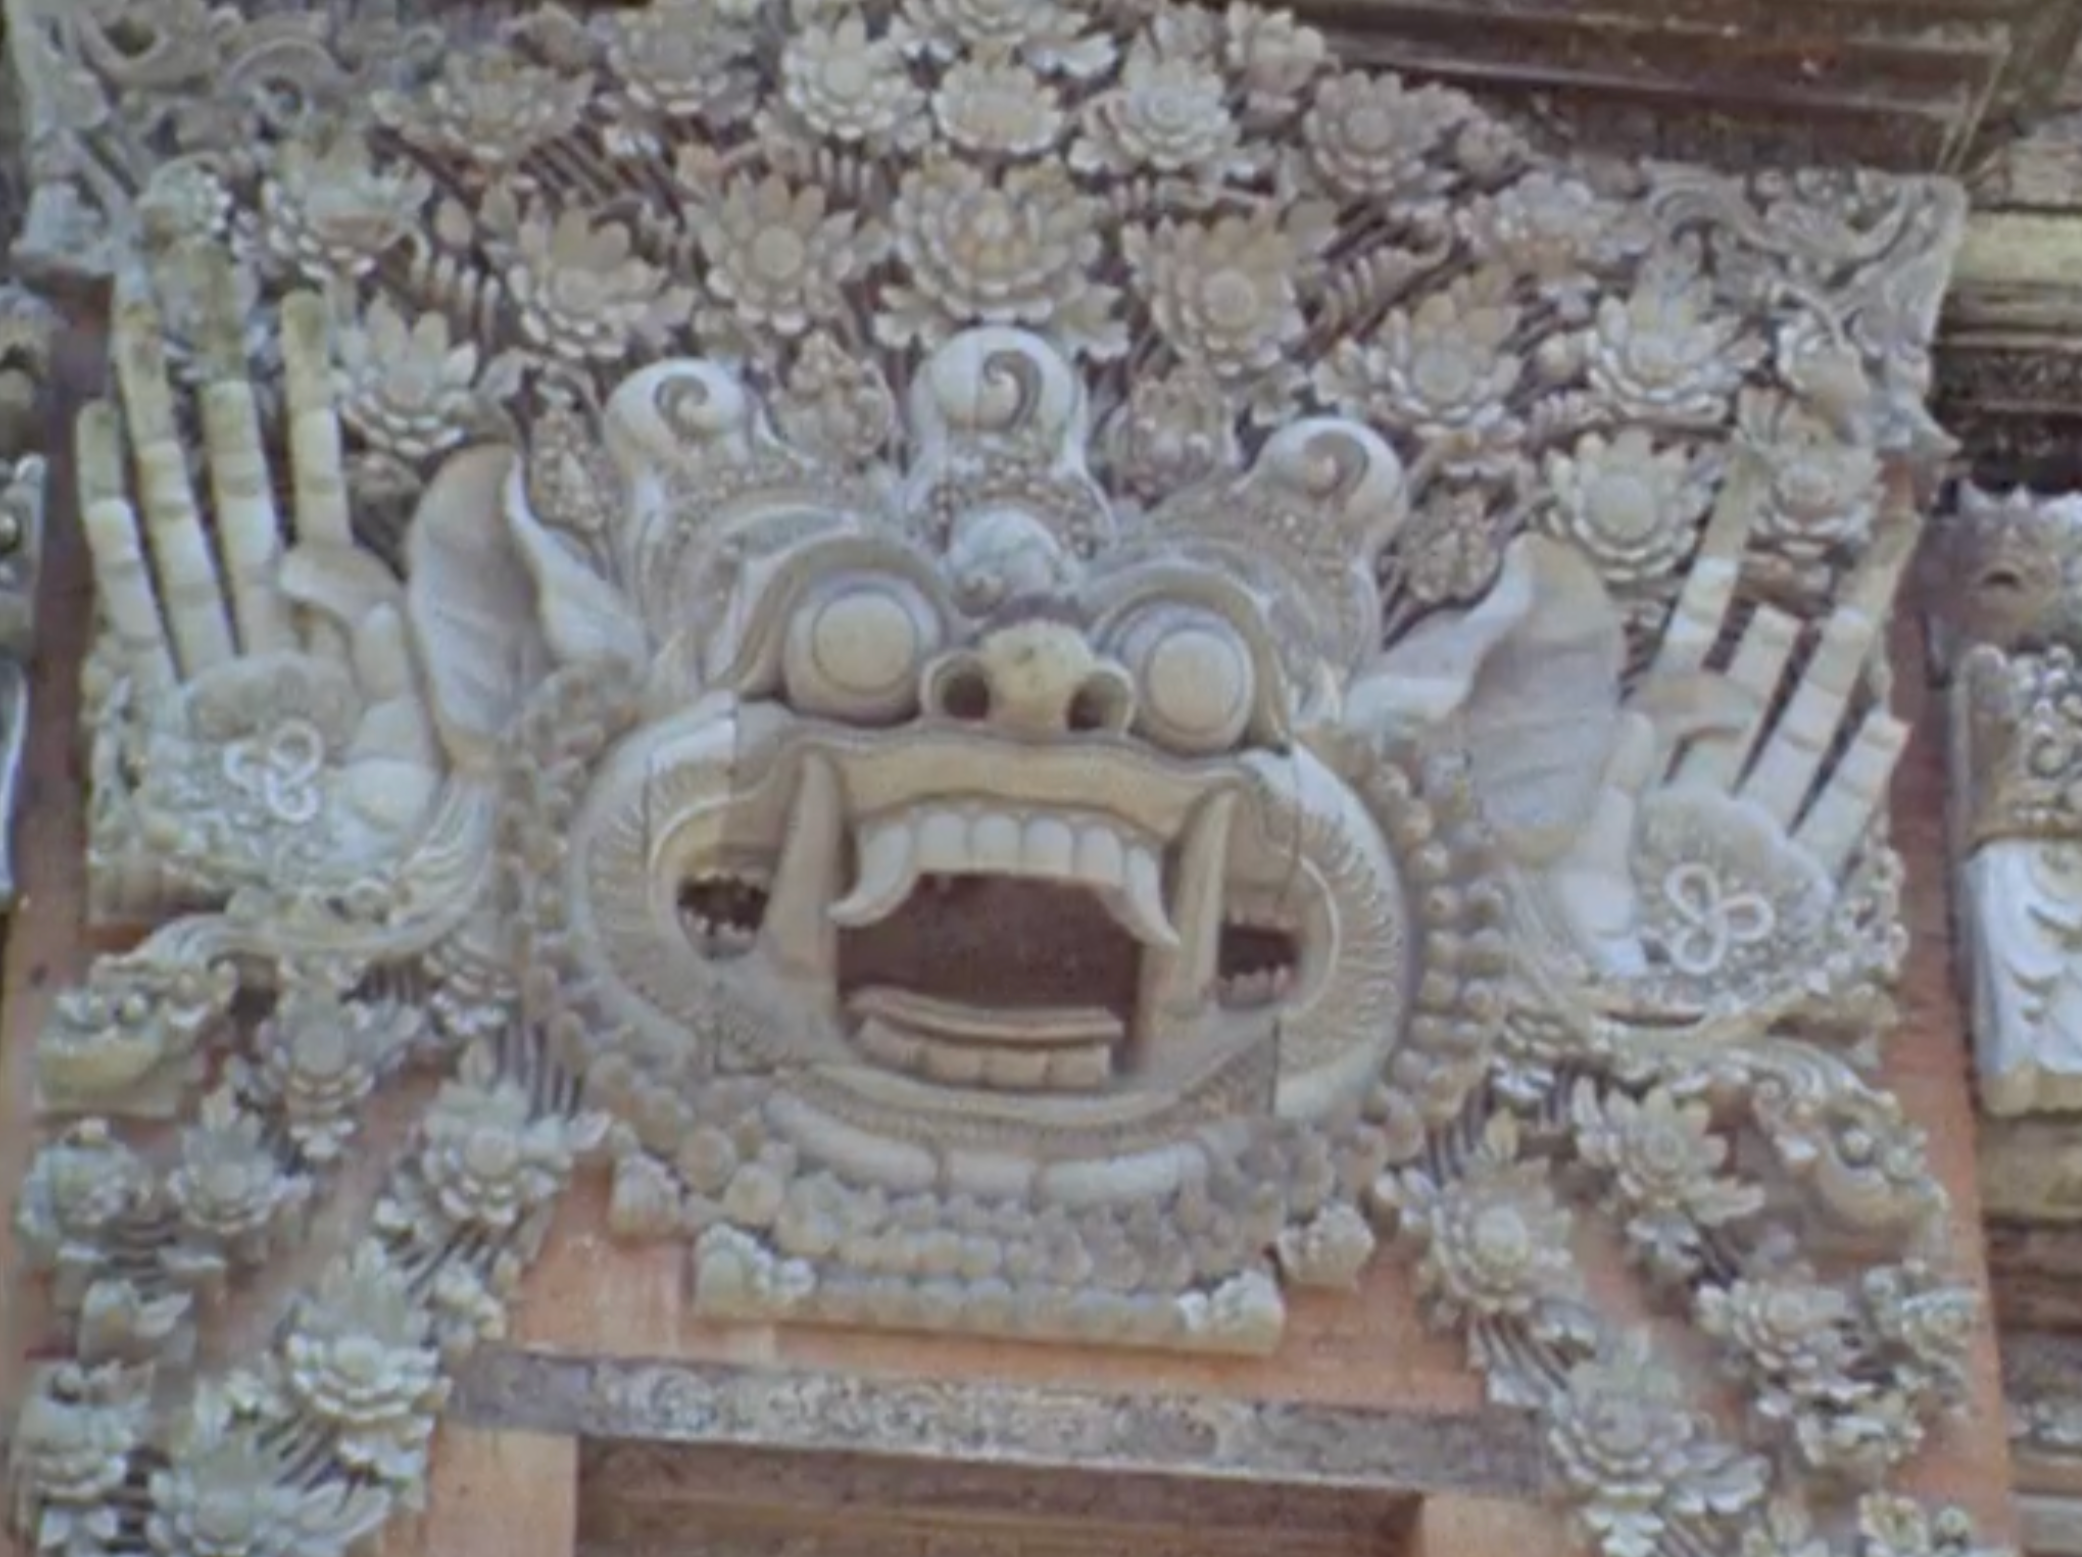
\includegraphics[width = 0.8\textwidth]{chapter1/bali}
\caption*{A carved image on the wall of a Balinese temple. Interesting how the face appears threatening, whilst also being surrounded by an emination of flowers. }
\end{figure}

\vspace{8pt}
\hrule
\vspace{8pt}

The content of this chapter is divided into two key sections accompanied by some more vapid topics of a more divergent nature.  Here is outlined the two key parts: 

\begin{itemize}
\item  \textbf{ Logistic speciation} In the spirit of Yule's 1924 paper and other more recent work with birth death processes, \cite{nee1994extinction} a continuous time Markov chain is formulated to model the production of species within a genus.  This model differs from the standard birth death process by having an inhomogeneous origination rate.  That is, the rate at which new species emerge is a function of time 
$$\beta(N(t)) $$
which is based on the relative availability of resources for a genus population which is expanding into a domain. The logistic model is used to describe the size of the population $N(t)$ in relation to its carrying capacity,  $K$  and this relative difference is taken to form the basis of the origination rate $\beta$. 


\item \textbf{ Pimentel fly model (cyclic competitive exclusion)}
"The ecological theatre and the evolutionary play" (G.  E.  Hutchinson) contains a summary of an experiment done by someone called Pimentel in the 50s.  It's purpose was to challenge the theory of competitive exclusion which states that two species can not simultaneously occupy the same niche.  It showed that an oscillation can arise when two species of fly occupy the same space provided that travel through the space is slowed by a series of compartments within the container.  This being because when one species gets pushed to near extinction,  it evolves more in response to infraspecific competitive interactions than those interspecific interactions with members of its group. \par 
This part of the chapter is about a model of these observed dynamics.\par
I also propose an addition to this model which aims to mirror the dynamic talked about in the Nietzsche quote (speciation being more prevalent when the species is the dominant of the two). 


\item \textbf{Allegorical model of rise run ruin and rejuvenation}
This is a model of one of the more vapid areas of this chapter.  The concept includes a quantity aiming to quantify potential (or vitality) in the system. This quantity,  $N(t)$ being high drives the emergence of species $\xt$.  But then, high $\xt$ count has the effect of reducing the potential.  Eventually as the quantity of allowance of "potential" per species $N/\xt$ becomes particularly low (its inverse being high), the rate of catastrophe increases to the point of certain collapse,  whereby $\xt$ declines suddenly to 0.  Subject then only to Poisson revival.  \par 

This is set up with the aim of representing something like the cyclic dissipative pattern of bifurcations seen in the example of stokes flow around a circle (oscillating turbulence shedding), and might also be seen in the rise and (sometimes sudden) fall of structures such as civilisations (speaking with reckless apocryphal speculation).  

\end{itemize}





\begin{figure}[h!]
\centering
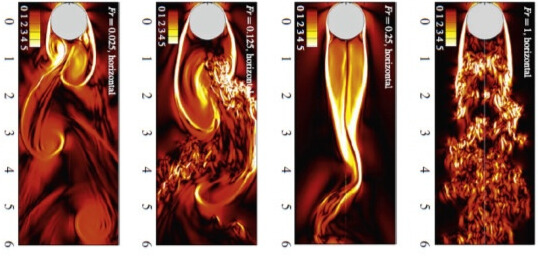
\includegraphics[width = 0.8\textwidth]{chapter1/Stokes}
\caption*{Stokes flow around a circle with cyclic turbulence shedding.}
\end{figure}





\subsubsection{Chapter 8: Conclusion}


This chapter begins with the pursuit of a curiosity.  The question of whether a replication rate advantage, weighted towards the beginning of a branching process will lead it to generally outperform another process without the front weighting.  I should specify that a condition is imposed whereby the two compared models have overall the same "replicative potential".  In the case of discrete time branching, this condition manifests in the sum of the dividing probabilities being the same over a defined number of generations. \par 

\vspace{10pt}
\noindent
The reason for this curiosity was to determine whether there is some fundamental advantage to replication being weighted towards the outset.  It turns out not to be the case; there is no advantage (in the expected value at least), provided the condition. \par 

In the case of Y. pestis seeking a replicative advantage in host macrophages,  the condition of equivalent overall replicative potential of course doesn't hold.  Because taking the higher rate at the outset doesn't diminish the rate of extracellular replication. \par 
The next part of this chapters explores stochastic birth death style models which encorporate two phases.



\vspace{15pt}
\noindent
\textbf{Two phase models}
The first phase in each of the following models represents the pro-phagocytosis phase of Y. pestis pathogenesis.  The second phase represents extracellular growth. \par

A few versions are explored: 

\begin{itemize}
\item \textbf{Birth-death to birth-death}
With two successive birth death processes, the duration of the first can be controlled directly as a parameter.  And this indirectly controlls the initial count in the second phase.


\item \textbf{Birth-death-catastrophe to birth-death-catastrophe}
In the case of an initial BDC process followed by birth death, the duration of the first phase is determined indirectly by the bursting rate. 

\item \textbf{Constant to birth-death}
Here,  the initial count of the second phase is controlled directly. This is the same as what was described in part of the the Mathematical bacground section (demonstrating the importance of initial counts in slightly supercrictical birth death processes).  The closer to criticallity (from above) the process, the more significant the effect.  And it seems straightforward to argue (which I hope to do elsewhere) that most biological replication processes,  if they are supercritical at all, opperate close to the critical threshold. (This is of course excepting cases where the early stages of a logistic groth phase are still causing more substantially exponential growth). 



\item \textbf{Constatnt to birth-subdusive-death}  A subducive death rate simply means a death rate which declines as a function of time.  This assumption follows loosly from a theory that over time, Y. pestis will after progresing through more and more generation cycles, begin to adapt to the particular environment of that host.  The presence of host-symbiotic immuno bacteriophages could form the basis of an example in which this dynamic applies.  In other words, the first Y. pestis may not be able to subvert the attacks of certain present bacteriophages, but maybe its great grandaughter can.  \par 
If a dynamic like this were present, it could have the effect of causing the extracellular net-replication rate to begin sub-critical, and tend into supercriticallity over time. In this case, a larger initial cohort would be of vital importance,  this possibly being provided by the within macrophage phase. 
\end{itemize}






\noindent
\textbf{Quadrant argument}
There is a simple argument for why Y.  pestis would favour phagocytosis to begin with and an anti-phagocytosis strategy  when neutrophil recruitment takes place: That neutrophils are more effective killers,  and so Y. pestis would want to avoid them.  But why not resist phgocytosis to begin with? Likely because the macrophage intracellular environment permits some replicative advantage. This section mathematizes this straightforwad argument using the simple birth death process. 


































































































%%%%%%%%%%




\chapter{Glossary of terms, objects and concepts}





\section{Chapter introduction}



\section*{Human innate immune system}


\subsection*{Macrophages}


\subsection*{Neutrophils}


\subsection*{Other leukocytes}


\subsection*{Complement}


\subsection*{Cytokines}


\subsection*{Lymphatic system}



\subsection*{Bacteriophages}









\section*{Mathematical concepts}



\subsection*{Branching criticallity}


\subsubsection*{Subcritical}


\subsubsection*{Supercritical}


\subsubsection*{Critical}





\subsection*{fffff}



\subsection*{fffff}



\subsection*{fffff}




\section*{Ggggg}



\subsection*{fffff}



\subsection*{fffff}

















\begin{figure}[h!]
    \centering
    % First row of two images
    \begin{subfigure}{0.48\textwidth}
        \centering
        \includegraphics[width=\textwidth]{chapter2/IMG_ch2/YPwebsite/web1}
    \end{subfigure}
    \hspace{\fill}
    \begin{subfigure}{0.48\textwidth}
        \centering
        \includegraphics[width=\textwidth]{chapter2/IMG_ch2/YPwebsite/web4}
    \end{subfigure}

    \vspace{0.5em} % Small vertical space between rows

    % Second row of two images
    \begin{subfigure}{0.48\textwidth}
        \centering
        \includegraphics[width=\textwidth]{chapter2/IMG_ch2/YPwebsite/web2}
    \end{subfigure}
    \hspace{\fill}
    \begin{subfigure}{0.48\textwidth}
        \centering
        \includegraphics[width=\textwidth]{chapter2/IMG_ch2/YPwebsite/web5}
    \end{subfigure}

    \vspace{0.5em} % Small vertical space between rows

    % Third row of two images
    \begin{subfigure}{0.48\textwidth}
        \centering
        \includegraphics[width=\textwidth]{chapter2/IMG_ch2/YPwebsite/web3}
    \end{subfigure}
    \hspace{\fill}
    \begin{subfigure}{0.48\textwidth}
        \centering
        \includegraphics[width=\textwidth]{chapter2/IMG_ch2/YPwebsite/web6}
    \end{subfigure}

    % Single caption for all images
    \caption{Here we see a schematic depiction of the stages of a Y. pestis infection. At first, mostly blue phase one units replicate within green macrophages. Over time, phase one bacteria become red, changing into phase two, and the macrophages begin to burst. In this javascript (p5.js) simulation, neutrophils are recruited on demand with the push of a button. They appear suddenly and quickly absorb all phase one units in their path, killing then rapidly once engulfed. In the final slide we see only phase two bacteria floating around the extracellular matrix, unabsorbed.}
    \label{fig:two_columns_six_images}
\end{figure}

































% Some notes on what is left to do
%
%  Chapter introduction 
%  Branching processes section 
%  Check and tidy QS stuff
%  Check and tidy survivor stuff
%  Check and tidy MOC stuff
%  Add simple BD derivation to the MOC section
%
%
%
%


























%%%%%%%%%%%%%%%%%%%%%%%%%%%%%%%%%%%%%%%%%%%%%%%%%%%%%%%%%%%%%%%%%%%%% Branching processes 




















\chapter{Mathematical background}


\begin{itemize}
\item In the case of slightly supercritical branching,  the initial count of replicative individuals weighs heavily on the chance of overall process survival.

\item In the case of subcritical branching,  when conditioning on process non-death, the expected individual count tends to a constant (a quasi-stationary mean).  The value of this, $\mean{\xt| \xt>0}$, grows to infinity in the limit of the process becoming critical from below.  In the case of the continuous time birth-death process, we can describe the inverse of this conditional mean with a formula; in the case of the discrete Galton-Watson process,  we tried to find the (yet unknown) equivalent formula.  Despite ultimately not finding it, we still think it is attainable.  
\end{itemize}





%%%%%%%%%%%%%%%%%%%%%%%%%%%%%%%%%%%%%%%%%%%%%%%%%%%%%%%%%%%%%%%%%%%%%%%%%%%%%%%%%%%%%%%%%%%%%%%%% Special 1 criticallity thing




\section{Limiting conditional distribution}



Suppose each individual produces, at the end of its life, independently, a number of offspring that is a random variable $\xx$, with 
$$\pr{\xx = k} = p_k, \hspace{20pt} k = 0,1,2,\dots$$
Denote the mean number of offspring per individual by 
$$\mu=\mean{\xx}$$
Let ${\bf Z}_n$ be the number of individuals in the $n$th generation. Then $\mean{\zz_n|\zz_0=1} = \mu^n.$ If $\mu < 1$ then $\lim_{n\to \infty}{\pr{\zz_n = 0}} = 1$. The population is guaranteed to go extinct.

Denote the probability generating function of $\xx$ as 
$$\phi(z) = \mean{z^{\xx}},$$
and the probability of population extinction by generation $n$ as 
$\pr{\zz_n = 0} = u_n.$
Then, as can be seen from a first step argument, it holds that 
\begin{equation}
\label{iterPGF}
u_{n+1} = \phi(u_n).
\end{equation}

\subsection{Death or division}
Consider the specific case: 
\begin{align*}
p_2 &= P &&\text{(division)}  \\
p_0 &= 1-P && \text{(death)}\\
p_i &= 0 \hspace{20pt} \forall i \neq 0,2  
\end{align*}

\noindent
In this case the mean number of offspring per individual takes the value,
$$\mu = 2P.$$
And so the expected population size resulting from a single offspring will be
$$\mean{\zz_n} = (2P)^n.$$
From (\ref{iterPGF}), we see
\begin{equation}
\label{unIter}
u_{n+1} = 1-P + P u_n^2.
\end{equation}
With $u_n$ the probability of extinction, let us also denote its complement
$$S_n = 1-u_n,$$
the probability of population persistence at generation $n$. 

From (\ref{unIter}), it can be shown that
\begin{equation}
\label{SnIter}
S_{n+1} = 2P S_n - PS_n^2.
\end{equation}

\subsection{Late time persistence probability, $S_n$}

Considering the case where $P < 0.5$, in which death of an individual is more probable than its reproduction, the expected population size will tend towards 0 with increasing $n$; the probability of non-extinction too will approach 0. 

As it does so, $S_n^2$ becomes insignificant in comparison to $S_n$. For this reason, the iterative relation, (\ref{SnIter}), will increasingly satisfy
\begin{equation}
\label{attenuated}
S_{n+1} \approx 2PS_n.
\end{equation}
So at late time ($n\to\infty$), it will be found that
\begin{equation}
\label{lateS}
S_n \sim A\,(2P)^n\qquad (n\to\infty),\quad A=\lim_{m\to\infty}S_m/(2P)^m.
\end{equation}
(The limit of $S_n$ itself is $0$ for $P<\tfrac12$; one must not write $\lim S_n = A(2P)^n$ as an ordinary limit identity.)
The multiplying constant, $A$, might be interpreted as those lingering conditions on $S_n$ accumulated before attenuation to (\ref{attenuated}). In any case, it can be demonstrated computationally: 


\begin{figure}[ht]
\centering
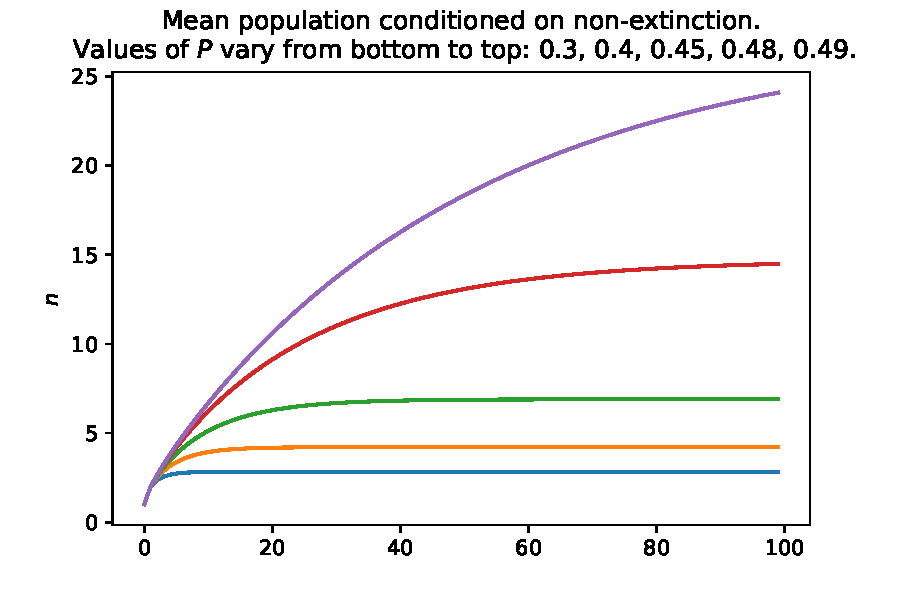
\includegraphics[width = 0.8\textwidth]{chapter3/IMG_ch3/conditionalMean.pdf}
    \label{fig:image}
\end{figure}

\noindent
Figure \ref{fig:image} shows $(2P)^n / S_n$ plotted over successive generations, $n$. In the code, $S_n$ is calculated iteratively using (\ref{SnIter}). The lines were generated with different values of $P$, those at the top closer to the critical state; the purple line was made with $P = 0.49$, the blue at the bottom, $P=0.3$. It is clear that this ratio will tend to a constant value towards large $n$.  

\subsection{Quasi-stationarity}

It is often the case in stochastic processes, as it is in this one for $P<0.5$, that fixation to a particular state is inevitable. Although, in certain cases, it can be observed that before absorption to some final state, behaviour becomes predictable according to some unchanging distribution. This phenomenon has been termed quasi-stationarity. 


\subsection{Mean}
Such behaviour can be observed in a population evolving by the update rules stated above. For demonstration, consider the mean number of individuals from a single ancestor, conditioned on non-extinction: 
$$\mean{\xx_n} = \pr{\xx_n =0} \cancelto{0}{\mean{\xx_n|\xx_n =0}}  + \pr{\xx_n \neq 0}\mean{\xx_n|\xx_n \neq0}.$$
It follows that 
$$\mean{\xx_n|\xx_n \neq 0} =\frac{\mean{\xx_n}}{\pr{\xx_n\neq 0}} = \frac{(2P)^n}{S_n} .$$ 
Then, due to (\ref{lateS}), as $n\to\infty$
$$\mean{\xx_n|\xx_n \neq 0} \to \frac{(2P)^n}{A(2P)^n} = \frac{1}{A};$$
At late time, the remaining non-extinct population tends to a constant expected size.

\subsection{Variance}

\subsubsection{Computing the second moment, $\mean{\xx_n^2}$}

For a random variable, $\xx$, the moment generating function is defined, $\mean{\ee^{t\xx}}$. It can also be written in terms of the probability generating function, $\phi(\ee^t)$. For variable, $\xx$ in question, the pgf is 
\begin{equation*}
\phi_1(z) = Pz^2 + (1-P),
\end{equation*}
and the mgf is 
\begin{equation}
\label{mgf1}
M_1(t) = \phi_1(\ee^t) = P\ee^{2t} + (1-P).
\end{equation}
The subscript 1 indicates relevance to generation $n = 1$. Moments are obtained from $M_n(t)$ in the following way.
\begin{equation}
\label{mgf2}
\mean{\xx_n^r} = \frac{\dd^r}{\dd t^r} M_n(t)\bigg|_{t=0}.
\end{equation}
For example, to get the second moment of $\xx_1$, we can differentiate (\ref{mgf1}) twice, and evaluate the result at $t=0$:
$$ \frac{\dd^2}{\dd t^2} M_1(t)\bigg|_{t=0} = 4P\ee^{2t}\big|_{t=0} = 4P.$$
Quantifying the process' second moment is important when it comes to computing the population variance for successive iterations. But this is only the second moment of the first generation size. To obtain its value for any generation $n$, we must dig a little deeper.  

Following (\ref{mgf2}), we seek to differentiate the moment generating function twice. To start with, let us represent the $n$th mgf in terms of probability generating functions. Recall,
$$\phi_n(z) = \underset{n \text{ times}}{\underbrace{ \phi_{1}\hspace{-2pt}\lrb{\phi_1\hspace{-2pt}\lrb{\dots\phi_1\hspace{-2pt}\lrb{z}}}    }}.$$  
So it follows that 
$$M_n(t) = \phi_1\lrbq{\phi_1\lrbq{\dots\phi_1\lrbq{\ee^t}}}.$$
Differentiating this once, 
\begin{equation}
\label{dmgf1}
M_n'(t) = \phi_1'\lrbq{\phi_{n-1}\lrbq{\ee^t}}  \cdot  \phi_1'\lrbq{\phi_{n-2}\lrbq{\ee^t}}  \cdots   \phi_1'\lrbq{\phi_{1}\lrbq{\ee^t}} \cdot \phi_1'\lrbq{\ee^t} \cdot\ee^t.
\end{equation}
Because 
$$\phi_1'\lrbq{\phi_k\lrbq{\ee^t}} = \frac{\dd}{\dd \phi_k\lrbq{\ee^t}}\bigg(P[\phi_k\lrbq{\ee^t}]^2 + (1-P)\bigg) = 2P \phi_k\lrbq{\ee^t},$$
and $\phi_1'\lrbq{\ee^t} = 2P\ee^t$, (\ref{dmgf1}) is equivalent to 
$$M_n'(t) = (2P)\phi_{n-1}\lrbq{\ee^t}  \cdot  (2P)\phi_{n-2}\lrbq{\ee^t} \cdots (2P)\phi_{1}\lrbq{\ee^t} \cdot (2P)\ee^{2t}.$$
Which in turn can be written as
\begin{equation}
\label{dmgf2}
M_n'(t) = (2P)^n \cdot M_{n-1}(t)  \cdot  M_{n-2}(t)  \cdots M_{1}(t)  \cdot \ee^{2t}.
\end{equation}
Before differentiating this a second time, it is instructive to note that each of the multiplied components, when evaluated at $t=0$ become 1; $M_k(0) = 1$ $\forall k$, and $\ee^{2\times 0} = 1$. 

So, when evaluating the second derivative at $t=0$, it will be seen that many of the parts simplify. This is because, with the expression being a combination of multiplied functions of $t$, differentiating by $t$ will result in a sum of terms. Each element of the sum will be like (\ref{dmgf2}), but with one of the components differentiated wrt t. This is just the product rule ---
\begin{align*}
M_n''(t) = (2P)^n\bigg[  &M_{n-1}'(t)  \cdot  M_{n-2}(t)  \cdots M_{1}(t)  \cdot \ee^{2t} \\
+ &M_{n-1}(t)  \cdot  M_{n-2}'(t)  \cdots M_{1}(t)  \cdot \ee^{2t} \\
&\hspace{65pt}\cdots\\
+ &M_{n-1}(t)  \cdot  M_{n-2}(t)  \cdots M_{1}'(t)  \cdot \ee^{2t} \\
+ &M_{n-1}(t)  \cdot  M_{n-2}(t)  \cdots M_{1}(t)  \cdot 2\ee^{2t} \bigg].
\end{align*}
And as most of the components become 1 with $t=0$,
\begin{equation*}
M_n''(0) = (2P)^n\lrbs{M_{n-1}'(0) + M_{n-2}'(0) + \cdots + M_1'(0) + 2}.
\end{equation*}
$M_k'(0)$ is simply the mean population at generation $k$, so
\begin{equation*}
M_n''(0) = (2P)^n\lrbs{(2P)^{n-1} + (2P)^{n-2} + \cdots + (2P) + 2} = (2P)^n\lrbs{\sum^{n-1}_{i = 0}\lrb{(2P)^i} + 1}.
\end{equation*}
Using the finite geometric series sum, $\sum_{i=1}^n r^{i-1} = (1-r^n)/(1-r)$, 
\begin{equation*}
\mean{\xx_n^2} = M_n''(0) = (2P)^n\lrbs{\frac{1-(2P)^n}{1-2P} + 1};
\end{equation*}
rearranging,
\begin{equation}
\label{secondMoment}
\mean{\xx_n^2}  = (2P)^n\lrb{1 + \frac{1}{1-2P}} - (2P)^{2n}\lrb{\frac{1}{1-2P}}.
\end{equation}
(The minus sign is required: at $n=1$ the expression must return $\mean{\xx_1^2}=4P$.)



\subsubsection{Late time variance}
Var($\xx_n$) is computed using $\mean{\xx_n^2} - \mean{\xx_n}^2$. With (\ref{secondMoment}), we can write,
$$\text{Var}(\xx_n) = (2P)^n\lrb{1 + \frac{1}{1-2P}} - (2P)^{2n}\lrb{\frac{1}{1-2P}} - (2P)^{2n}.$$
For $2P < 1$, at large $n$, $(2P)^{2n}$ will become insignificant in comparison to $(2P)^n$. Hence, as $n\to\infty$,
$$\text{Var}(\xx_n) \to (2P)^n\lrb{1 + \frac{1}{1-2P}}.$$
It's tempting to jump straight from this, to a conclusion that the variance conditional on $\xx_n \neq 0 $ is stationary. But let's not get ahead of ourselves and start from the conditional moments:
$$\mean{\xx_n^2|\xx_n\neq 0} = \frac{\mean{\xx_n^2}}{S_n} \xrightarrow{n\to\infty}   \frac{(2P)^n\lrb{1 + \frac{1}{1-2P}}}{A(2P)^n} = A^{-1}\lrb{1 + \frac{1}{1-2P}}$$
$$\mean{\xx_n|\xx_n\neq 0} =  \frac{\mean{\xx_n}}{S_n}  \xrightarrow{n\to\infty}    \frac{(2P)^n}{A(2P)^n} = A^{-1}$$
From this, it can be seen that the conditional variance will indeed tend to a constant value at late time:
\begin{equation*}
\text{Var}(\xx_n|\xx_n\neq0) = \frac{1}{A}\lrb{1+\frac{1}{1-2P}} - \frac{1}{A^2}.
\end{equation*}



\subsection{Quantifying the quasi-stationary distribution}

We are yet to compute the constant $A$, but so far, Grant has shown that (\ref{SnIter}) can be written as 
$$S_{n+1} - S_n = -rS_n - PS_n^2,$$
($r = 1-2P$). Which in the large $n$ limit will satisfy
$$\frac{\dd S(x)}{\dd x} = -(1-2P)S_n = PS^2,$$
a Riccati equation with solution
$$S(x) = \frac{rB}{e^{rx} +- PB},$$
$B$ constant. 




































%%%%%%%%%%%%%%%%%%%%%%%%%%%%%%%%%%%%%%%%%%%%%%%%%%%%%%%%%%%%%%%%%%%%% special 2 small




\section{Survivability of small populations}
Consider the basic Galton Watson process where each cell leaves behind two daughters or dies. And for the sake of example, suppose it is also near critical --- either sub or super.\par With the probability of individual replication $p$, and death $1-p$ each close to a half. A lineage will die out at its first round almost half the time. Should it pass one generation, both of its two offspring will die in their first attempt with around probability $0.25$. And so, the lineage of that initial cell will persist as far as the third generation only with a likelihood of approximately $0.375$;

\begin{multline}
\sim0.375 = (1\;-\;\sim0.5)(1\;-\;\sim0.5\;\times\;\sim0.5) =\\ (\text{neither extinction at first step})\times(\text{nor at the second}).
\end{multline}

\noindent
Generally, the chance of a process surviving to a given generation can be quantified using the probability generating function (pgf), $\phi(z) = \sum_i P_i z^i$; $P_i$ being the likelihood of an individual leaving behind $i$ offspring. Extinction by the $n$th step, $u_n$, is obtainable through iteration of the pgf:
$$u_{n+1} = \phi(u_n).$$
In our case, the pgf is $\phi(z) = pz^2 - 1-p$, and so both the extinction and survival ($S_n = 1-u_n$) likelihoods can be computed as follows. 

\begin{equation}
\label{ext}
u_{n+1} = pu_n^2 - 1-p
\end{equation} 
$$S_{n+1} = 2pS_n - p S_n^2$$
(going out sequentially from the initial $u_n = 0$ and $S_n = 1$). Using (\ref{ext}), we can simply compute the extinction probabilities for a given initial individual which undergoes critical branching: for generations $n=$ 0, 1, 2, 3, $\dots$, and $u_n$= 0.5, 0.625, 0.695, 0.741 (3 s.f.). Hence, the likelihood of process survival decays quickly with ongoing rounds of replication:

\begin{center}
  \begin{tikzpicture}[scale = 3]
    % Scatter plot points
    \foreach \x/\y/\color in {1/0.55/red, 2/0.4386250/red, 3/0.3766719/red, 4/0.336304/red,
                                                1/0.5/black, 2/0.375/black, 3/0.3046875/black, 4/0.25827/black,
                                                   1/0.449999/blue, 2/0.313874/blue, 3/0.2381546/blue, 4/0.188816/blue}
      \fill[color=\color] (\x, \y) circle (1pt);

    % Trajectories
    \draw[red, thick] (0, 1) -- (1, 0.55) -- (2, 0.4386250) -- (3,0.3766719) -- (4,0.336304);
    \draw[black, thick] (0, 1)--(1,0.5) --  (2,0.375) -- (3,0.304687) -- (4,0.25827);
    \draw[blue, thick] (0, 1)--(1,0.449999)  --  (2,0.313874) -- (3,0.238154) -- (4,0.18881);

    % Axis labels
    \draw[-] (0,0) -- (4.3,0) node[right] {$n$};
    \draw[-] (0,0) -- (0,1.15) node[above] {$S_n$};

    % Time points
    \foreach \x/\label in {0/0, 1/1/, 2/2/, 3/3, 4/4}
      \node at (\x, -0.18) {\label};
      
      \foreach \y/\label in {0/0, 0.5/0.5, 1/1/}
      \node at (-0.15, \y) {\label};
  \end{tikzpicture}

\end{center}



\subsection*{An initial infectious cohort of size $k$}
Now suppose that $X_0 = k$. Instead of the process beginning with a single unit, it starts out with a group; and for the sake illustration, we can assume this bunch is small to moderate in number, perhaps around $k = 10$.\par Given we assume supercritical branching, as the bacterial count increases, the population growth will naturally become more predictably exponential in nature. A large number of cohort units causing the expected dynamics to shine through, emergent from the haze of individual stochasticity.\par


And so, for or this initial colony --- maybe $k = 10$ pathogenic bacteria in a mammalian host --- what are its chances of persistence? Of going on to found a full blown infection?  \par
We can address this question by considering the probability with time that at least one descendent remains from the first colony. This is the likelihood that not every lineage has gone extinct. Given a single lineage dies out with the above described probability, ${}_1u_n$, the chance of all $k$ lineages dissapearing is $\lrb{{}_1u_n}^k$. Hence the probability of population persistence, in at least some descendant, is 
$$S^{(k)}_n = 1 - \lrb{{}_1u_n}^k.$$


\begin{figure}
\centering
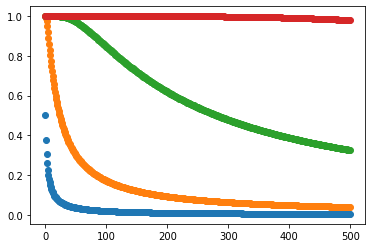
\includegraphics[width=0.6\textwidth]{chapter3/IMG_ch3/kvals.png}
\caption{Survival probability out to 500 generations with 1, 10, 100, and 1000 initial individuals. (From blue to red).  }
\label{fig1}
\end{figure}

\noindent
Figures \ref{fig1} and \ref{fig2} show the values of $S_n^{(k)}$ through 500 generation for $k$ = 11, 10, 100, and 1000. The effect seen in figure \ref{fig1}, that a greater first cohort gives improved longevity, is highly sensitive to the criticality of the process. So persistence develops quickly as $p$ approaches 0.5 from below, and it continues to improve dramatically into supercriticality. To illustrate this, figure \ref{fig2} shows the same experiment done with $p$ slightly above and below 0.5. 



\begin{figure}
\centering

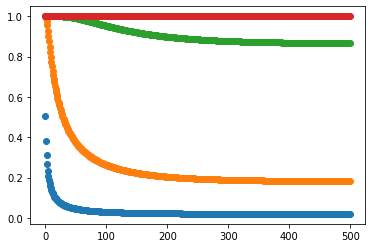
\includegraphics[width=0.45\textwidth]{chapter3/IMG_ch3/kvals505.png}
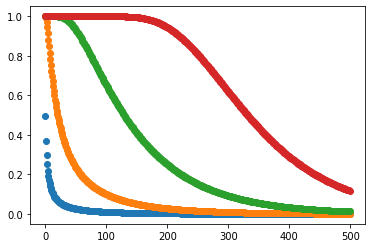
\includegraphics[width=0.45\textwidth]{chapter3/IMG_ch3/kvals495.png}
\caption{Like figure \ref{fig1} but the value of $p$ is no longer exactly critical at 0.5. On the left, it is supercritical at 0.505; for the right, 0.495. }
\label{fig2}
\end{figure}

\subsection*{Potential implications}

Firstly, it seems if nothing else a curiosity, that this observation aligns with a point made be R. Mann in a recent paper on modelling the longevity and size of phylogenetic clades. Here it was highlighted that those clades which have persisted through the ages, and are often of superior diversity, happened to have experienced an above average early rate of species origination. As far as I understand, this is an observation from the fossil record itself. Mann et al. argued that this empirical fact can be explained merely as a statistical consequence. As, if you were to run, as they did, a large number of homogeneous birth death processes, and select only those which happen to survive to some arbitrary large positive time ---  ``the present''. 





A hypothesis: It is of pathogenic advantage for an agent to ensure a high security of early initial replication, even at some cost to individual unit survival through later generations. 


\subsection{Discrete Birth-death-catastrophe --- does it have a stationary limiting distribution?}

Until the point of catastrophe, a discrete time BDC process will exhibit the same behaviour with regards to its stationary conditional limiting distribution as the basic Galton Watson model. \par
So conditioning on non-rupture, the process, when also conditioned on non extinction by death, exhibits a stationary limiting distribution. Does this mean that there will be a quasi-stationary distribution when conditioning on neither death nor catastrophe. In any case, we can test this with simulations.\par
But in addition, it will prove helpful to figure out some probability of non-catastrophe with advancing generations.
\subsection*{Probability of rupture at step $n$}

If the probability that a given individual will initiate catastrophe is $k$, the we can specify the probability that none of a size $N$ cohort will do so at an iterative step. A single individual will not cause rupture with probability $1-k$, two wp $(1-k)^2$, three, $(1-k)^3$, so on and so forth... \par
Considering for now the case of only birth and catastrophe --- no death --- it can be said with certainty the census of a living population at arbitrary generation, $n$. With a single progenitor, it is simply the case that the population will double at each step prior to catastrophe. Hence, the process will come to its abrupt halt in generation $n$ with probability
$$1-(1-k)^{2^{n-1}}$$
(not every individual didn't cause catastrophe).

\subsection*{Probability of process survival}
Thinking along these lines we can define (for the no death case)  the probability that a process survives to generation $n$. Lets call it $S_n$. For generation 0, this is clearly certain ($S_0=1$). Survival to generation one simply requires that the first individual replicated, $S_1 = (1-k)$. For persistence to step 2, not only must the first unit divide, but so must each of its offspring: $$S_2 = (1-k)(1-k)^2.$$ And so a pattern can be seen. For survival to the $n$th generation, every step prior must have been passed. Hence,
$$S_n = \Pi_{i = 0}^{n-1} (1-k)^{2^i} = (1-k)^{\sum^{n-1}_{i=0}2^i}.$$

\subsection*{Death included}
The difficulty comes in defining $S_n$ when death is allowed. In this version, the size of a living population can no longer be known with certainty through the generations. The question I would now like to address, is do the probabilities some how ``shake out'' when the expected value of the process is used; is the following correct? 
$$S_n  = (1-k)^{\sum^{n-1}_{i=0}\mean{\xx_i}}.$$
I suspect it isn't. But probably worth checking. 


\subsection{Continuous time birth death --- Survival probability and QS distribution}


From Linda Allen's book, we have the probability of extinction for the simple birth death process: 
$$p_0(t) = \begin{cases}
\lrb{\frac{\mu - \mu e^{(\mu - \lambda) t }}{  \lambda  - \mu e^{(\mu - \lambda) t }}}^N, \;\; &\lambda \neq \mu\\ 
\lrb{\frac{\lambda t}{1 + \lambda t}}^N, \;\;& \lambda = \mu.
\end{cases}$$
From this, we also have the probability of process survival at time $t$:
$$S^{(N)}(t) = 1 - p_0(t)$$

\subsection*{Limiting mean conditioned on non-extinction}
The simple birth-death model has a stationary mean when $\mu < \lambda$. We can demonstrate this simply in the following way. The conditional mean can be obtained via,
\begin{equation}
\label{condit}
\mean{\xt | \xt > 0} = \frac{\mean{\xt} }{S^{(N)}(t)}.
\end{equation}
And the late time limit of this can be evaluated using L'hopital's rule. When $\mu < \lambda$, 
$$\lim_{t\to\infty}\mean{\xt | \xt > 0}  = \frac{\mu}{\mu - \lambda} = \frac{1}{1 - \frac{\lambda}{\mu}}$$

\subsection*{More simply}

Taking $N=1$, when $\lambda < \mu$: 
$$\mean{\xt } = \ee^{(\lambda - \mu)t}$$
and,
\begin{align*}
S(t) &= 1 - \lrb{\frac{\mu - \mu \ee^{(\mu - \lambda)t}}{\lambda - \mu \ee^{(\mu-\lambda)t}}} \\
&= \frac{\lambda - \mu}{\lambda - \mu \ee^{(\mu - \lambda)t}}.
\end{align*}
So given (\ref{condit}),
$$\mean{\xt | \xt > 0} = \frac{\lambda\ee^{(\lambda-\mu)t} - \mu}{\lambda - \mu}.$$
In the case considered, $\lambda > \mu$, the limiting conditional mean becomes a constant:
$$\lim_{t\to\infty}\mean{\xt | \xt > 0}  = \frac{\mu}{\mu - \lambda}  \lrb{ = \frac{1}{A}}$$.
This may be represented as
$$\frac{1}{A} = \frac{1}{1 - \frac{\lambda}{\mu}};$$
and writing in terms of replication probability, $p = \lambda/(\lambda + \mu)$,
$$\frac{1}{A} = \frac{1-p}{1-2p};$$
inverse of the quasi-stationary mean,
$$A = \frac{1-2p}{1-p}.$$


\begin{center}
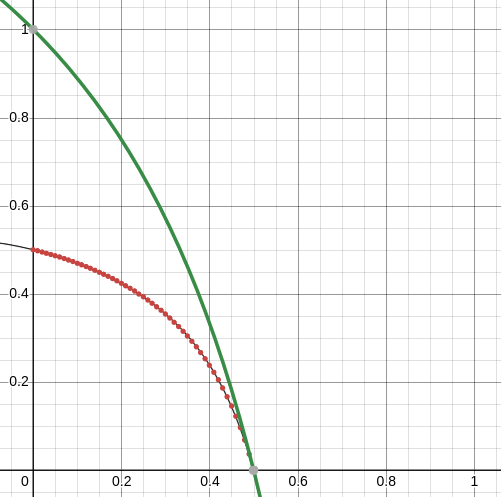
\includegraphics[width=0.45\textwidth]{chapter3/IMG_ch3/dtctA.png}
\end{center}

\noindent
In the figure above, the green line is $A$ as defined above. The red dots represent precise numerically obtained values of the analogous measure in the discrete time Galton Watson process; the black line is a closely matching formula found computationally \cite{cohen2024physics} \cite{stanley2002evolving}.\par
The obvious question which comes to mind is: why does the curve start at 1 in continuous time and 0.5 in discrete time. Merely dividing the ``green'' formula by 2 doesn't cause an overlap.





























%%%%%%%%%%%%%%%%%%%%%%%%%%%%%%%%%%%%%%%%%%%%%%%%%%%%%%%%%%%%%%%%%%%%%%%%%%%%%%%%%%%%%%%%%%%%%%%%%%%%%%%%%% MOC





\section{Method of characteristics}




In previous work, we have been successful in describing birth-death dynamics of pathogenic particles inside a host cell which can rupture. In future, we wish to extend this understanding to cases with multiple host cells sharing a medium. Setting up a model with more than one host requires consideration of what happens when the first one ruptures. The shared medium suddenly gains a potentially large cohort of pathogenic particles, available for subsequent absorption by remaining hosts. We have begun to develop the analysis under the assumption of what may be called ``immediate transfer'' --- the whole pathogenic contents of a rupturing cell being relocated to the intracellular environment of another host. This is quite a hard assumption. Another, perhaps more realistic restriction might be to incorporate an ``absorption period'': following a host cell rupture, absorption events relocate the pathogenic cohort between remaining hosts. Then, only when every pathogen has been taken in, do birth death and rupture continue. 

Working towards an understanding of such ``absorption models'', we can begin by considering processes where a pathogenic cohort infiltrate only a single host cell. 

\subsection{Only absorption} 
Perhaps the most simple case for an absorption process is that of a single host cell, able to take-in pathogenic particles, but in which no subsequent dynamics take place --- without any birth, or death of pathogen within the host. 

We can introduce the variables $\xt$ \& $\yt$ to represent the number of pathogenic particles within, and outside of the host cell respectively. The same labelling will be used in later versions of the single-host model. In all cases, events will be assumed to be stochastic, happening between exponentially distributed inter-event times. This property arises from the assumption that event-rates are time-independent. It then follows that our continuous-time stochastic process, $\{(\xt, \yt) : t\in[0,\infty\}$, conforms to the memoryless Markov property.

With only absorption to consider, the model can be specified by the following probabilities --- outcome-likelihoods over an infinitesimal duration, $\Delta t$ (taken in the limit to 0).
%\begin{equation}
  % \begin{split}
  %   \pr{\Delta\xx= 1,\;\Delta\yy = -1 \;|\; \yt = j} = j \alpha \Delta t\\
 %    \pr{\Delta\xx= 0,\;\Delta\yy = 0 \;|\; \yt = j} = 1 -  j \alpha \Delta t
 %  \end{split}
%\label{probSpec1}
%\end{equation} 
\begin{align*}
     \pr{\Delta\xx= 1,\;\Delta\yy = -1 \;|\; \yt = j} &= j \alpha \Delta t,  &&\text{(absorption)}\\
     \pr{\Delta\xx= 0,\;\Delta\yy = 0 \;|\; \yt = j} &= 1 -  j \alpha \Delta t,  &&\text{(no event)}
\end{align*} 


\noindent
where $\Delta \xx = \xx_{t+\Delta t} - \xt$ (same for $\yy$). Notice the multiplication by $j$, the number of extracellular particles --- each unit subjected to the same probability, $\alpha \Delta t$, of being taken up. 

The model's initial condition will be specified: $\xx_0 = 0$, $\yy_0 = N$. A starter population of census $N$ occupying the extracellular medium. 

Defining state probabilities, $p_{i,j}(t) = \pr{\xt = i,\; \yt = j}$, we can write down the forward Kolmogorov equations: 
\begin{equation}
\label{F1}
\ddt{\p} = \alpha(j + 1) p_{i-1,j+1} - \alpha j \p.
\end{equation}

\noindent
Then, with the probability generating function defined,
\begin{equation}
\label{pgfDef}
G(x,y,t) = \sum_i\sum_j \pt x^iy^j 
\end{equation}

\noindent
$\left(=\mathbb{E}\left[x^{\xt}y^{\yt}\right]\right)$, we can go on to derive a PDE for $G(x,y,t)$ in the following way. 

Firstly, multiply each equation in (\ref{F1}) by $x^iy^j $,
\begin{equation*}
%\label{pdeDerev1}
\pddt{\p x^iy^j} = \alpha(j + 1) p_{i-1,j+1}x^iy^j - \alpha j \p x^iy^j.
\end{equation*}

\noindent
Then sum over $i$ and $j$ for non-zero $\pt$,
\begin{equation}
\label{pdeDere2}
\sum_{i = 0}^N\sum_{j=0}^N\pddt{\p x^iy^j} = \alpha\sum_{i = 1}^{N+1}\sum_{j=-1}^{N-1}(j + 1) p_{i-1,j+1}x^iy^j - \alpha \sum_{i = 0}^N\sum_{j=0}^Nj \p x^iy^j.
\end{equation}

\noindent
(Note, for any $i, j > N$, and when $i+j \neq N$, $\pt = 0$ $\forall t$. This is because pathogenic particles in this model are neither created nor destroyed.)

Rearranging (\ref{pdeDere2}), we find 
\begin{equation*}
\label{pdeDerev2}
\sum_{i = 0}^N\sum_{j=0}^N\pddt{\p x^iy^j} = \alpha\left(x\sum_{i = 0}^N\sum_{j=0}^N j p_{i,j}x^{i}y^{j-1} -  y\sum_{i = 0}^N\sum_{j=0}^Nj \p x^iy^{j-1} \right),
\end{equation*}

\noindent
which can be written in terms of the following partial derivatives,
\begin{equation*}
\label{pdeDerev2}
\sum_{i = 0}^N\sum_{j=0}^N\pddt{\p x^iy^j} = \alpha\left(x - y\right)\sum_{i = 0}^N\sum_{j=0}^N \pdd{\p x^iy^j}{y}.
\end{equation*}

\noindent
Notice, with (\ref{pgfDef}), 
\begin{equation}
\label{PDE1}
\pddt{G(x,y,t)} = \alpha\left(x - y\right) \pdd{G(x,y,t)}{y};
\end{equation}

\noindent
the chosen initial condition corresponding to $G(x,y,0) = y^N$.
 
This first-order linear initial value problem, it turns out, proves quite difficult to solve. The method of characteristics, though practicable by definition on equations of three variables, has so far lead only to mystification.

But, as it happens, we can obtain its solution via other means. 

\subsubsection*{Benefits of the independence property}
$G(x,y,t)$, as referred to above was specific to the initial condition, $\xx_0 = 0$, $\yy_0 = N$. We may further specify the probability generating function,
\begin{equation*}
G_n(x,y,t) = \sum_i\sum_j \pr{\xt = i,\;\yt=j \;|\;\xx_0 = 0,\;\yy_0=n } x^i y^j.
\end{equation*}
In such a process of just absorption, each of the $N$ pathogenic particles will get taken up by the host cell one by one. If we were to focus our attention on a single particle of this cohort, the behaviour observed would not depend on the movements of it's neighbours. Due this property of independence, our variables $\xt$ \& $\yt$ can be thought of as the sum of $N$ sub-variables, $\xt^{(k)}$ \& $\yt^{(k)}$, each pertaining only to the movements of a single pathogenic unit: 
\begin{align*}
\xt = \xt^{(1)} + \xt^{(2)} + \dots + \xt^{(n)}\\
\yt = \yt^{(1)} + \yt^{(2)} + \dots + \yt^{(n)}
\end{align*}
This observation allows us to prove that 
\begin{equation}
\label{indRelPGF}
G_n(x,y,t) = \lrb{G_1(x,y,t)}^n:
\end{equation}
\begin{align*}
G_n(x,y,t) &= \ex{x^{\sum_{k=1}^n \xt^{(k)}} y^{\sum_{k=1}^n \yt^{(k)}}}\\
&=  \ex{\prod_{k=1}^n x^{\xt^{(k)}} \prod_{k=1}^n y^{\yt^{(k)}} }\\
&=  \prod_{k=1}^n\ex{ x^{\xt^{(k)}} y^{\yt^{(k)}} }\\
&=  \prod_{k=1}^n G_1(x,y,t)\\
&= \left(G_1(x,y,t)\right)^n
\end{align*}

\noindent
Now, consider there were only one pathogenic particle to begin with; $\xx_0 = 0$, $\yy_0 = 1$. It would after some time be absorbed, and this would be the final state of the system. No other states could be reached --- quite simply: $\pt = 0$ $\forall t$ for $i+j \neq1$.\par
We can hence fully determine the state probabilities of this simple case using the forward Kolmogorov equations.
\begin{align*}
\ddt{p_{0,1}(t)} = -\alpha p_{0,1}(t) && \ddt{p_{1,0}(t)} = \alpha p_{0,1}(t) 
\end{align*}
$\implies$
\begin{align*}
p_{0,1}(t) = \ee^{-\alpha t} && p_{1,0}(t) = 1 - \ee^{-\alpha t}
\end{align*}





\begin{figure}[H]
\begin{center}
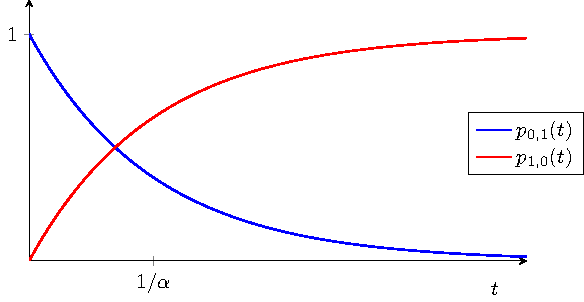
\includegraphics[width = 0.65\textwidth]{chapter3/IMG_ch3/abs1.pdf}
\end{center}
\end{figure}








\noindent
Given these represent the only two non-zero state probabilities of the single particle system, we can write-out the associated probability generating function as
\begin{align*}
G_1(x,y,t) &= p_{1,0}(t)x + p_{0,1}(t)y\\
    &=   \lrb{1-\ee^{-\alpha t} }x + \ee^{-\alpha t}y.
\end{align*}
Then, applying relation (\ref{indRelPGF}), we can define the probability generating function for this absorption-only system generally, for any initial state,
\begin{equation*}
G_n(x,y,t) = \lrb{ \lrb{1-\ee^{-\alpha t} }x + \ee^{-\alpha t}y}^n;
\end{equation*}

\noindent
noting that this does satisfy equation (\ref{PDE1}) along with its initial condition, 
$$G_n(x,y,0) = y^n.$$


%- forward kolmogorov equations

%- PDE for probability generating function 

%- note on difficulty in solving it

%- Solution allowed by independence assumption.

 
\subsection{Absorption-death}

In reality, when resident in a host-cell, pathogenic particles may be subject to death. \par
Setting-up a model as above, with $\xt$ \& $\yt$ representing the count of intracellular and extracellular pathogen, we can incorporate particle death with the following addition. 
\begin{align*}
     \pr{\Delta\xx= 1,\;\Delta\yy = -1 \;|\; \yt = j} &= j \alpha \Delta t,  &&\text{(absorption)}\\
      \pr{\Delta\xx= -1,\;\Delta\yy = 0 \;|\; \xt = i} &= i \mu \Delta t,  &&\text{(death)}\\
     \pr{\Delta\xx= 0,\;\Delta\yy = 0 \;|\; \yt = j, \xt=i} &= 1 -  \lrb{ j\alpha + i\mu}\Delta t,  &&\text{(no event)}
\label{probSpec1}
\end{align*} 

Form here, an analogous line of reasoning can be followed. A familiar difficulty is found on arrival at the first order linear PDE,
\begin{equation*}
\label{PDE2}
\pddt{G(x,y,t)} = \mu(1-x) \pdd{G(x,y,t)}{x}+\alpha\left(x - y\right) \pdd{G(x,y,t)}{y}.
\end{equation*}

\noindent
This point being reached from a similar derivation using the forward Kolmogorov equations:
\begin{equation*}
\label{FK1}
\ddt{\p} = \alpha(j + 1) p_{i-1,j+1} + \mu(i+1)p_{i+1,j} - (\alpha j + \mu i) \p.
\end{equation*}

\noindent
But as above, the solution can be constructed with a work-around employing the relation 
\begin{equation*}
G_n(x,y,t) = \lrb{G_1(x,y,t)}^n.
\end{equation*}

\noindent
As before, individual particles are independent from one another in their movements.\par
Without birth events, the maximum number of particles in the system is restricted to it's initial value. So, when considering the case of an isolated pathogenic unit, the probability generating function takes its form,
\begin{equation*}
G_1(x,y,t) = p_{0,0} + p_{1,0}x + p_{1,0}y.
\end{equation*}

\noindent
These state-probabilities can be determined as follows using the forward Kolmogorov equations. 
\begin{align*}
\ddt{p_{0,1}(t)} = -\alpha p_{0,1}(t) && \ddt{p_{1,0}(t)} = \alpha p_{0,1}(t) - \mu p_{1,0}(t)
\end{align*}
$\implies$
\begin{align*}
p_{0,1}(t) = \ee^{-\alpha t} && p_{1,0}(t) = \frac{\alpha}{\mu - \alpha} \Big(   \ee^{-\alpha t} - \ee^{-\mu t} \Big) && p_{0,0}(t) = 1 -p_{0,1}(t)  -p_{1,0}(t) 
\end{align*}





\begin{figure}[H]
\begin{center}
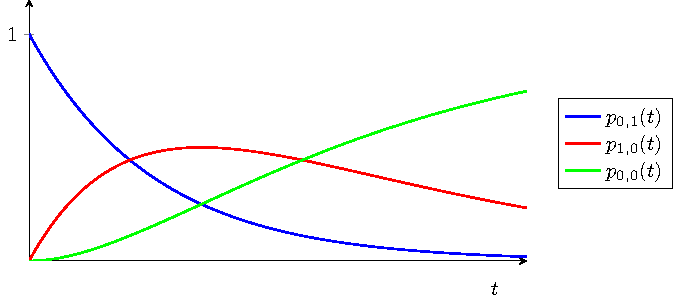
\includegraphics[width = 0.65\textwidth]{chapter3/IMG_ch3/abs2.pdf}
\end{center}
\caption{Caption}
\end{figure}
    

    


\noindent
Leading, as above, to the general probability generating function, $G_n(x,y,t)$, through relation (\ref{indRelPGF}):
\begin{equation*}
G_n(x,y,t) = \lrb{1-\frac{\mu}{\mu - \alpha}  \ee^{-\alpha t}  + \frac{\alpha}{\mu - \alpha} \ee^{-\mu t}  + \frac{\alpha}{\mu - \alpha} \Big(   \ee^{-\alpha t} - \ee^{-\mu t} \Big)x +  \ee^{-\alpha t} y}^n
\end{equation*}



%\begin{equation}
%G_1(x,y,t) = 1-\frac{\mu}{\mu - \alpha}  \ee^{-\alpha t}  + \frac{\alpha}{\mu - \alpha} \ee^{-\mu t}  + \frac{\alpha}{\mu - \alpha} \Big(   \ee^{-\alpha t} - \ee^{-\mu t} \Big)x +  \ee^{-\alpha t} y
%\end{equation}

\subsection{Method of characteristics (absorption-death)}

Before continuing to the case of absorption-birth-death where replication may occur within the host cell, let us revisit absorption-death from the point of its PDE for $G(x,y,t)$.  

\begin{equation}
\label{PDE2}
\pddt{G(x,y,t)} = \mu(1-x) \pdd{G(x,y,t)}{x}+\alpha\left(x - y\right) \pdd{G(x,y,t)}{y},
\end{equation}
with initial condition $G(x,y,0) = y^N$.

Since writing the above sections, I have been given advice by Benjamin Sharp on how to use the method of characteristics for 3 variate problems.\par
We begin by introducing a change of variables $(x,y,t) \to (s,r,\tau)$:
$$G(x,y,t) = G\big(x(s,r,\tau), y(s,r,\tau), t(s,r,\tau) \big) \equiv G(s,r,\tau)$$
The method works by seeking solutions on the characteristic surfaces of constant $s$ and $r$; $G(\tau)$. To do so, we must introduce an initial surface in the $s$, $r$, $\tau$ space:
\begin{align}
\label{ICpar}
x(s,r,0) = s && y(s,r,0) = r && t(s,r,0) = 0
\end{align}

With the probability generating a function of only one variable, $\tau$, we can write down the characteristic equations as ODEs. First, consider,
\begin{equation*}
\dda{G}{\tau} = \pddt{G} \dda{t}{\tau}  +  \pdd{G}{x}\dda{x}{\tau} + \pdd{G}{y}\dda{y}{\tau} .
\end{equation*}
Notice similarity with (\ref{PDE2}),
$$0  = -\pddt{G} + \mu(1-x)\pdd{G}{x} + \alpha (x-y)\pdd{G}{y}.$$
Comparing coefficients, we can write down the characteristic ODEs: 
\begin{align}
\dda{G}{\tau} &= 0\label{ch11}\\
\dda{t}{\tau} &= -1\label{ch12}\\
\dda{x}{\tau} &= \mu(1-x)\label{ch13}\\
\dda{y}{\tau} &= \alpha(x-y)\label{ch14}
\end{align}


\subsubsection*{(\ref{ch11})}
Solving the first characteristic equation,
$$\dda{G}{\tau} = 0$$
$$G = \phi(s,r)$$
$\phi$ constant on surfaces of constant $s$, and $r$.\par
With  (\ref{ICpar}), the initial condition on $G$ translates to $G(s,r,\tau=0) = r^N$, which informs us that $\phi(s,r) = r^N$. Hence,
\begin{equation}
\label{GrN}
G(s,r,\tau) = r^N.
\end{equation}



\subsubsection*{(\ref{ch12})}
$$\dda{t}{\tau} = -1$$
$$t = -\tau + c(s,r)$$
Using (\ref{ICpar}), we can fix the constant, $c(s,r) = 0$.
\begin{equation}
\label{minustau}
t = -\tau
\end{equation}


\subsubsection*{(\ref{ch13})}
$$\dda{x}{\tau} = \mu(1-x)$$
$$\vdots$$
$$1-x = c(s,r) \ee^{-\mu \tau}.$$
With initial condition, (\ref{ICpar}), $c(s,r) = 1-s$;
\begin{equation}
\label{sandxwithtau}
1-x = (1-s) \ee^{-\mu \tau}.
\end{equation}


\subsubsection*{(\ref{ch14})}

\begin{align*}
\dda{y}{\tau} &= \alpha(x-y)\\
\dda{y}{\tau} &= \alpha\left(1-(1-s) \ee^{-\mu \tau} -y\right)
\end{align*}
$$\vdots$$
$$y = 1 - \frac{\alpha}{\alpha-\mu}(1-s)\ee^{-\mu\tau} + c(s,r)\ee^{-\alpha\tau}.$$
Applying (\ref{ICpar}), $c(s,r) = r + \frac{\alpha}{\alpha-\mu}(1-s) -1$;
\begin{equation}
\label{ywithr1}
y = 1 - \frac{\alpha}{\alpha-\mu}(1-s)\ee^{-\mu\tau} + \lrb{r + \frac{\alpha}{\alpha-\mu}(1-s) -1}\ee^{-\alpha\tau}.
\end{equation}

\vspace{15pt}
\noindent
Finally, if we rearrange (\ref{ywithr1}) for $r$, also substituting $s(x,y,t)$ from (\ref{sandxwithtau}), and $\tau = -t$ from (\ref{minustau}), we find:
\begin{equation*}
r = 1-\frac{\mu}{\mu - \alpha}  \ee^{-\alpha t}  + \frac{\alpha}{\mu - \alpha} \ee^{-\mu t}  + \frac{\alpha}{\mu - \alpha} \Big(   \ee^{-\alpha t} - \ee^{-\mu t} \Big)x +  \ee^{-\alpha t} y
\end{equation*}
Then, with $G = r^N$ ((\ref{GrN})), this matches the solution obtained in the previous section, 
\begin{equation*}
G(x,y,t) = \lrb{1-\frac{\mu}{\mu - \alpha}  \ee^{-\alpha t}  + \frac{\alpha}{\mu - \alpha} \ee^{-\mu t}  + \frac{\alpha}{\mu - \alpha} \Big(   \ee^{-\alpha t} - \ee^{-\mu t} \Big)x +  \ee^{-\alpha t} y}^N.
\end{equation*}





\subsection{Absorption-birth-death}

Introducing replication for particles inside the host cell, we will see that though the independence property is still present, it no longer serves as a work-around in finding the probability generating function $G(x,y,t)$. This is because, given a single initial infections particle, with birth events, an infinite number of states can be reached. Hence $G_1(x,y,t)$ will be constituted by an infinite number of terms.\par

Thankfully, we are now also equipped to solve the PDEs for $G(x,y,t)$, and this is the approach we will take.\par

Setting up the model like in previous cases, $\xt$ \& $\yt$ represent the counts of intracellular and extracellular pathogenic particles. Birth events are added to the transition rates as follows.

\begin{align*}
     \pr{\Delta\xx= 1,\;\Delta\yy = -1 \;|\; \yt = j} &= j \alpha \Delta t,  &&\text{(absorption)}\\
     \pr{\Delta\xx= 1,\;\Delta\yy = 0 \;|\; \xt = i} &= i \beta \Delta t,  &&\text{(birth)}\\
      \pr{\Delta\xx= -1,\;\Delta\yy = 0 \;|\; \xt = i} &= i \mu \Delta t,  &&\text{(death)}\\
     \pr{\Delta\xx= 0,\;\Delta\yy = 0 \;|\; \yt = j, \xt=i} &= 1 -  \lrb{ j\alpha + i\mu + i\beta}\Delta t,  &&\text{(no event)}
\label{probSpec1}
\end{align*} 

The forward Kolmogorov equation is written as such.
\begin{equation*}
\label{FK3}
\pddt{\p } = \alpha(j + 1) p_{i-1,j+1} + \mu(i+1)p_{i+1,j}  +  \beta(i-1)p_{i-1,j}    -  (\alpha j + \mu i+\beta i) \p 
\end{equation*}

From here, again, with reasoning seen above, we can derive the associated PDE for $G(x,y,t)$.

\begin{equation}
\pddt{G} = \lrb{\mu - (\mu+ \beta)x + \beta x^2}\pdd{G}{x} + \alpha(x-y)\pdd{G}{y}
\end{equation}

To solve this by the method of characteristics, as above we re-parametrize $(x,y,t)$ to $(s,r,\tau)$, then seek solutions on characteristic surfaces of constant $s$ and $r$. Doing so brings us to the characteristic ODEs: 
\begin{align}
\dda{G}{\tau} &= 0\label{ch21}\\
\dda{t}{\tau} &= -1\label{ch22}\\
\dda{x}{\tau} &= \mu-(\mu+\beta)x + \beta x^2\label{ch23}\\
\dda{y}{\tau} &= \alpha(x-y)\label{ch24}
\end{align}
Applying the same initial conditions on $(s,r,\tau)$ as above in (\ref{ICpar}), we can solve these equations as follows.

\subsubsection*{(\ref{ch21}) \& (\ref{ch22})}
Like in the previous section the first two characteristic equations yield: 
$$G(s,r,\tau) = \phi(s,r),$$
and ultimately,
\begin{equation}
\label{gngngn}
G(s,r,\tau) = r^N.
\end{equation}
Then,
$$t = -\tau.$$   


\subsubsection*{(\ref{ch23})}
This equation looks remarkably like Jonty's equation for $S$, the survival probability. 
$$\dda{x}{\tau} = \beta\lrb{x-x_+}\lrb{x-x_-}$$
with,
$$x_{\pm} = \frac{\mu + \beta}{2\beta} \pm \sqrt{\lrb{\frac{\mu + \beta}{2\beta}}^2 - \frac{\mu}{\beta}}.$$
The main difference in its solution with Jonty's equation comes with an $s$ when fixing the constant of integration:
\begin{equation}
x(\tau) = \frac{x_+(s-x_-) - x_-(s-x_+)\ee^{\beta(x_+-x_-)\tau}}{(s-x_-) - (s-x_+)\ee^{\beta(x_+-x_-) \tau}}
\label{xabd}
\end{equation}


\subsubsection*{(\ref{ch24})}
The last characteristic equations is
$$\dda{y}{\tau} = \alpha(x-y).$$
To solve this we will need to substitute $x$ as found above, (\ref{xabd}). With an integrating factor, the equation becomes,
$$\dda{}{\tau}\lrb{\ee^{\alpha\tau} y} = \alpha \ee^{\alpha\tau} x(\tau).$$
Integrating with respect to $\tau$,
$$\ee^{\alpha\tau }y = \alpha\int \ee^{\alpha\tau} \frac{x_+(s-x_-) - x_-(s-x_+)\ee^{\beta(x_+-x_-)\tau}}{(s-x_-) - (s-x_+)\ee^{\beta(x_+-x_-) \tau}} \dd\tau.$$ 
Then splitting the numerator, 
\begin{align}
\label{bigdoubleints}
\ee^{\alpha\tau }y &=  \alpha x_+(s-x_-) \int \frac{ \ee^{\alpha \tau} } {(s-x_-) - (s-x_+)\ee^{\beta(x_+-x_-) \tau}}\dd\tau \notag \\ 
&-\alpha x_-(s-x_+)\int\frac{\ee^{\left[ \alpha + \beta(x_+-x_-) \right]\tau}}{(s-x_-) - (s-x_+)\ee^{\beta(x_+-x_-) \tau}}\dd\tau.
\end{align}

\noindent
Each of these integrals can be written in the form,
\begin{equation*}
I(\tau) = \int\frac{\ee^{h\tau}}{p+q\ee^{k\tau}}\dd\tau.
\end{equation*}
where $h$, $k$, $p$, $q$ are all constants. For example, in the first integral, $h = \alpha$, $k = \beta(x_+ - x_-)$, $p = (s-x_-)$, and $q = -(s-x_+)$. As it happens, we can solve this integral with: 
\begin{equation}
\label{hypIden}
I(\tau) = \frac{\ee^{h\tau}}{ph} {}_2F_1\lrb{1,\frac{h}{k};\frac{h}{k}+1; -\frac{q}{p}\ee^{k\tau}} + \text{const}.
\end{equation}
${}_2F_1(a,b;c;z)$ being the hypergeometric function, defined,
\begin{equation*}
{}_2F_1(a,b;c;z) =\sum^\infty_{n=0}\frac{(a)_n(b)_n}{(c)_n}\frac{z^n}{n!},
\end{equation*}
and $(p)_n$ is the (rising) Pochhammer  symbol:
$$(p)_n = \begin{cases} 1 &n=1\\
p(p+1)\cdots(p+n-1) &n>1
\end{cases}
$$
See appendix \ref{appxa} for a detailed derivation of (\ref{hypIden}).\par
Picking up again at (\ref{bigdoubleints}), the integrals are specified by (\ref{hypIden}):\\
(using $b_1 = \beta(x_+ - x_-)$ for convenience)
\begin{equation*}
\int \frac{ \ee^{\alpha \tau} } {(s-x_-) - (s-x_+)\ee^{b_1 \tau}}\dd\tau =  \frac{\ee^{\alpha\tau}}{\alpha(s-x_-)} {}_2F_1\lrb{1,\frac{\alpha}{b_1 };\frac{\alpha}{b_1 }+1; \frac{(s-x_+)}{(s-x_-)}\ee^{b_1  \tau}},
\end{equation*}
and
\begin{equation*}
\int\frac{\ee^{\left[ \alpha +b_1\right]\tau}}{(s-x_-) - (s-x_+)\ee^{b_1 \tau}}\dd\tau =   \frac{\ee^{(\alpha+b_1 )\tau}}{(\alpha+b_1 )(s-x_-)} {}_2F_1\lrb{1,\frac{\alpha + b_1 }{b_1 };\frac{\alpha + b_1 }{b_1 }+1; \frac{(s-x_+)}{(s-x_-)}\ee^{b_1  \tau}}.
\end{equation*}
Referring to these formulas as $I_1(s,r,\tau)$ and $I_2(s,r,\tau)$ respectively, and substituting into (\ref{bigdoubleints}): 
\begin{equation}
\label{eywithconst}
\ee^{\alpha\tau }y = \alpha x_+(s-x_-)I_1(s,r,\tau) - \alpha x_- (s-x_+) I_2(s,r,\tau) + \text{const}.
\end{equation}
From her, our initial condition, $y(s,r,0) = r$, fixes the constant ---
$$\text{const} = r -  \alpha x_+(s-x_-)I_1(s,r,0) + \alpha x_- (s-x_+) I_2(s,r,0).$$ 
Then, with a rearrangement of (\ref{eywithconst}), 
\begin{equation*}
r = \ee^{\alpha\tau }y - \alpha x_+(s-x_-)I_1(s,r,\tau) + \alpha x_- (s-x_+) I_2(s,r,\tau) +  \alpha x_+(s-x_-)I_1(s,r,0) - \alpha x_- (s-x_+). I_2(s,r,0)
\end{equation*}
With $I_1$, $I_2$ written explicitly,
\begin{align*}
r &= \\
 &\ee^{\alpha\tau }y\\ 
 &- \lrb{x_+ \ee^{\alpha\tau}}{}_2 F_1 \lrb{1,\frac{\alpha}{b_1 };\frac{\alpha}{b_1 }+1; \frac{(s-x_+)}{(s-x_-)}\ee^{b_1  \tau}}\\
&+\lrb{\frac{\alpha  }{\alpha + b_1}x_-\ee^{(\alpha + b_1)\tau}}{}_2F_1\lrb{1,\frac{\alpha + b_1 }{b_1 };\frac{\alpha + b_1 }{b_1 }+1; \frac{(s-x_+)}{(s-x_-)}\ee^{b_1  \tau}}\\
&+ \lrb{x_+}{}_2 F_1 \lrb{1,\frac{\alpha}{b_1 };\frac{\alpha}{b_1 }+1; \frac{(s-x_+)}{(s-x_-)}}\\
&- \lrb{\frac{\alpha  }{\alpha + b_1}x_-}{}_2F_1\lrb{1,\frac{\alpha + b_1 }{b_1 };\frac{\alpha + b_1 }{b_1 }+1; \frac{(s-x_+)}{(s-x_-)}}
\end{align*}

\noindent
From (\ref{xabd}), we have the relation,
$$\lrb{\frac{s-x_+}{s-x_-}} = \lrb{\frac{x-x_+}{x-x_-}}\ee^{b_1\tau},$$
which, applied to  the above, along with the switch, $\tau = -t$, yields 

\begin{align*}
r &= \\
 &\ee^{-\alpha t }y\\ 
 &- \lrb{x_+ \ee^{-\alpha t}}{}_2 F_1 \lrb{1,\frac{\alpha}{b_1 };\frac{\alpha}{b_1 }+1; \frac{(x-x_+)}{(x-x_-)}}\\
&+\lrb{\frac{\alpha  }{\alpha + b_1}x_-\ee^{-(\alpha + b_1)t}}{}_2F_1\lrb{1,\frac{\alpha + b_1 }{b_1 };\frac{\alpha + b_1 }{b_1 }+1; \frac{(x-x_+)}{(x-x_-)}}\\
&+ \lrb{x_+}{}_2 F_1 \lrb{1,\frac{\alpha}{b_1 };\frac{\alpha}{b_1 }+1; \frac{(x-x_+)}{(x-x_-)}\ee^{b_1  t}}\\
&- \lrb{\frac{\alpha  }{\alpha + b_1}x_-}{}_2F_1\lrb{1,\frac{\alpha + b_1 }{b_1 };\frac{\alpha + b_1 }{b_1 }+1; \frac{(x-x_+)}{(x-x_-)}\ee^{b_1  t}}
\end{align*}

\noindent
Finally, with (\ref{gngngn}),
\begin{align*}
G(x,y,t) &=\\
 &\Bigg[\ee^{-\alpha t }y\\ 
 &- \lrb{x_+ \ee^{-\alpha t}}{}_2 F_1 \lrb{1,\frac{\alpha}{b_1 };\frac{\alpha}{b_1 }+1; \frac{(x-x_+)}{(x-x_-)}}\\
&+\lrb{\frac{\alpha  }{\alpha + b_1}x_-\ee^{-(\alpha + b_1)t}}{}_2F_1\lrb{1,\frac{\alpha + b_1 }{b_1 };\frac{\alpha + b_1 }{b_1 }+1; \frac{(x-x_+)}{(x-x_-)}}\\
&+ \lrb{x_+}{}_2 F_1 \lrb{1,\frac{\alpha}{b_1 };\frac{\alpha}{b_1 }+1; \frac{(x-x_+)}{(x-x_-)}\ee^{b_1  t}}\\
&- \lrb{\frac{\alpha  }{\alpha + b_1}x_-}{}_2F_1\lrb{1,\frac{\alpha + b_1 }{b_1 };\frac{\alpha + b_1 }{b_1 }+1; \frac{(x-x_+)}{(x-x_-)}\ee^{b_1  t}}\Bigg]^N
\end{align*}


The following fact offers only some consolation from the unwieldiness of this formula.

$${}_2F_1\lrb{1,\delta;\delta+1;z} = \sum^\infty_{n=0}\frac{(1)_n(\delta)_n}{(\delta+1)_n}\frac{z^n}{n!} = \sum^\infty_{n=0}\frac{\delta}{\delta+n}{z^n}. $$

True, because along with $(1)_n = n!$, it can also be seen that 

$$\frac{(\delta)_n}{(\delta+1)n} = \frac{\delta\cancel{(\delta+1)}\cdots\cancel{(\delta + n-2)}\cancel{(\delta + n-1)}}{\cancel{(\delta+1)}\cancel{(\delta+2)}\cdots\cancel{(\delta + n-1)}(\delta + n)} = \frac{\delta}{\delta+n}.$$








\subsection*{Appendix}

\subsection{Deriving the integral result (\ref{hypIden})}\label{appxa}
To demonstrate result, 
$$\int\frac{\ee^{h\tau}}{p+q\ee^{k\tau}}\dd\tau= \frac{\ee^{h\tau}}{ph} {}_2F_1\lrb{1,\frac{h}{k};\frac{h}{k}+1; -\frac{q}{p}\ee^{k\tau}} + \text{const},$$
we will use the hypergeometric integral identity:

\begin{equation}
\label{idenHyp}
{}_2F_1(a,b;c;z) = \frac{\Gamma(c)}{\Gamma(b)\Gamma(c-b)}\int^1_0 u^{b-1}(1-u)^{c-b-1}(1-zu)^{-a} \dd u
\end{equation}
($\Gamma(x)$, being the standard gamma function). 

Taking the integral,
$$I(\tau) = \int\frac{\ee^{h\tau}}{p+q\ee^{k\tau}}\dd\tau.$$
Begin by applying the substitution, $v = \ee^{k\tau}$; with $\dd\tau = k^{-1}v^{-1} \dd v$.
\begin{align*}
I(v(\tau)) &= \frac{1}{k}\int\frac{v^{\frac{h}{k}}}{p+qv}v^{-1}\dd v\\
\notag\\
&= \frac{1}{pk}\int\frac{v^{\frac{h}{k}-1}}{1+\frac{q}{p}v}\dd v.
\end{align*}
Re-writing this as a definite integral from 0 to $v$ using a dummy variable, $s$,
$$I(v(\tau)) = \frac{1}{pk}\int^v_0\frac{s^{\frac{h}{k}-1}}{1+\frac{q}{p}s}\dd s.$$
Then, changing variables again with $s = vu$ (as $v$ is constant with regards to the definite integral, $\dd s = v\dd u$).
\begin{align}
I(v(\tau)) &= \frac{1}{pk}\int^1_0\frac{(vu)^{\frac{h}{k}-1}}{1+\frac{q}{p}vu} v \dd u\notag\\
\notag\\
&= \frac{v^{\frac{h}{k}}}{pk}\int^1_0\frac{u^{\frac{h}{k}-1}}{1+\frac{q}{p}vu}  \dd u.\label{backat}
\end{align}

\noindent
We see, this integrand lines up with that of the identity, (\ref{idenHyp});
\begin{equation*}
\int^1_0u^{\frac{h}{k}-1}(1-u)^0 \left(1-\left(-\frac{q}{p}v\right) u\right)^{-1} \dd u= \int^1_0 u^{b-1}(1-u)^{c-b-1}(1-zu)^{-a} \dd u.
\end{equation*}

\noindent
Notice, $b = \frac{h}{k}$, $c = \frac{h}{k}+1$,  $a = 1$,  and $z = -\frac{q}{p}v$. Hence,
\begin{align*}
\int^1_0\frac{u^{\frac{h}{k}-1}}{1+\frac{q}{p}vu}  \dd u &= \frac{\Gamma\left(\frac{h}{k}\right) \Gamma\lrb{1}}{\Gamma\lrb{\frac{h}{k} +1}} {}_2F_1\lrb{1,\frac{h}{k};\frac{h}{k}+1; -\frac{q}{p}v}\\
\notag\\
&= \frac{k}{h} {}_2F_1\lrb{1,\frac{h}{k};\frac{h}{k}+1; -\frac{q}{p}v},
\end{align*}
and, with (\ref{backat}),
\begin{equation*}
I(v(\tau)) = \frac{v^{\frac{h}{k}}}{ph}{}_2F_1\lrb{1,\frac{h}{k};\frac{h}{k}+1; -\frac{q}{p}v}.
\end{equation*}
Finally,
$$I(\tau) = \frac{\ee^{h\tau}}{ph}{}_2F_1\lrb{1,\frac{h}{k};\frac{h}{k}+1; -\frac{q}{p}\ee^{k\tau}}\hspace{17pt} (+ \text{const}).$$


\subsection{Extracting coefficients from the PGF -- a special case}

For a probability generating function defined not in terms of a series sum --- for example, 
\begin{equation}
\label{examplePgf}
G(t;x,y) =  \lrb{\lrb{1-\ee^{-\alpha t}}x + \ee^{-\alpha t}y}^n
\end{equation}
--- it is possible to make a conversion to its equivalent of the form,
\begin{equation}
\label{series1}
G(t;x,y) = \sum^{\infty}_{i=0}\sum^{\infty}_{j=0} p_{i,j}(t)x^iy^j.
\end{equation}
Thus extracting the time-dependent state probabilities, $p_{i,j}(t)$. It is required only that the formula $G(t;x,y)$ can be partially differentiated continuously in $x$ and $y$.\par
Here's why: A bivariate generalisation of the Maclaurin expansion can be written,
$$f(x,y)\approx Q(x,y) = \sum^{\infty}_{k=0} \lrb{\frac{1}{k!} \sum^{\infty}_{r=0}{k \choose r} \partial_x^r \partial_y^{k-r}f\bigg |_{(0,0)} x^r y^{k-r} }. $$
So, the coefficients of (\ref{series1}) can be generated via,
\begin{equation}
\label{stateProb}
p_{i,j}(t) = \lrb{i!j!}^{-1} \partial_x^i \partial_y^{j}f\big |_{(0,0)}.
\end{equation}

\subsection*{A special case}


For a probability generating function of the form,
$$G(t;x,y) = \lrb{c(t) + f(t) x + g(t) y}^n,$$
its partial derivatives in $x$ and $y$ can be obtained through
$$\partial_x^a\partial_y^b G = \lrbs{nf(t)}^a\lrbs{ng(t)}^bG.$$
With these derivatives, the state probabilities can be extracted using (\ref{stateProb}):
\begin{equation}
\label{stateProbSpec}
p_{i,j}(t) = \lrb{i!j!}^{-1} \lrbs{nf(t)}^i\lrbs{ng(t)}^jG(0,0).
\end{equation}
In this special case, $G(0,0) = (c(t))^n;$
\begin{equation}
\label{stateProbSpec2}
p_{i,j}(t) = \lrb{i!j!}^{-1} \lrbs{nf(t)}^i\lrbs{ng(t)}^j\lrbs{c(t)}^n.
\end{equation}
\subsection*{Applied to PGFs from absorption only and absorption-death }
Taking (\ref{examplePgf}), for example:
$$p_{i,j}(t) = \frac{n^{i+j}}{\lrb{i!j!}} \lrbs{1-\ee^{-\alpha t}}^i\lrbs{\ee^{-\alpha t}}^j.$$
The same can be done for 
$$G(t;x,y) = \lrb{1-\frac{\mu}{\mu - \alpha}  \ee^{-\alpha t}  + \frac{\alpha}{\mu - \alpha} \ee^{-\mu t}  + \frac{\alpha}{\mu - \alpha} \Big(   \ee^{-\alpha t} - \ee^{-\mu t} \Big)x +  \ee^{-\alpha t} y}^n$$
from the absorption-death case:
$$p_{i,j}(t) = \frac{n^{i+j}}{\lrb{i!j!}} \lrbs{\frac{\alpha}{\mu - \alpha} \Big(   \ee^{-\alpha t} - \ee^{-\mu t} \Big)}^i\lrbs{\ee^{-\alpha t}}^j\lrbs{1-\frac{\mu}{\mu - \alpha}  \ee^{-\alpha t} + \frac{\alpha}{\mu - \alpha} \ee^{-\mu t}}^n.$$


























\chapter{Birth death catastrope -- Definition and main results}





\section{Chapter introduction}











We aim to understand the stochastics of those infections which exploit a lytic mechanism in their initial pathogenesis. That is to say, infectious agents which utilize intracellular environments to their proliferative advantage.\par

The importance of stochasticity can not be understated, because during the initial handful of replicative cycles, there is an exaggerated 
chance of an infection dying out before it gets started. Were we to use deterministic modeling, this perilous beginning is at risk of being glossed over with variable bacterial counts venturing between 1 and 0. \par

Hence, to really grasp the significance of \textit{why} Y. pestis, and other pathogens do what they do, we must account for the interplay of chance and fortune. 

It is for this reason we have selected the birth death catastrophe process as a tool of inquiry. \par
\vspace{25pt}




\noindent
Study of the birth death catastrophe (BDC) process and its dynamics will form a central focus of this thesis. Here
we present a series of results and analysis associated with its behaviour. As a continuois-time discrete-state Markov chain, 
the BDC process found its origin in a paper by Brokwell et. al. published 1982. During the late 1970s and early 80s,
attempts were being made to describe unpredictable population collapses using stochastic process theory:
\begin{quotation}
    "There has recently been a great deal of interest in the development and
    analysis of stochastic models for the growth of populations which are subject to
    catastrophes due either to death or large-scale emigrations" (Brockwell et. al. 1982)
\end{quotation}
Prior to that work models had largely incorporated deterministic growth interspersed by stochastic reductions --- sudden
drops, the sizes and times of which defined in distribution (Pakes et. al 1979). These suffered from peculiarities of 
modelling discrete populations with continuous random variables, and so attempts were made to to employ a step process; 
continuous time Markov chains in discrete state space.\par

Actually, the model presented in this 1982 paper is a generalisation of what we refer to as the BDC process. Not only
did it also include immigration events --- single steps-up occuring as a Poisson process with constant rate --- but also, the
catastrophic steps down in population count were sized as random i.i.d variables, with a few basic distributions investigated.
In our case, the catastrophe event is taken to reduce the population directly to 0, or to a special post catastrophe state,
$H$; in either case causing fixation.


Our interest in the Birth Death Catastrophe process stems from an application from within-host infection modelling. Like others before, we were interested in the pathogenesis behaviour of intracellular replication and bursting. Our agent of focus, Y. Pestis,
finds its way into host macrophaegs and replicates there, before ultimately lysing the cell so that the population of
infectious bacteria can traverse the extracellular matrix and continue their exploitative fight for survival.
"Catastrophe" here terms the cell-bursting event, which becomes increasingly likely as the intracellular population expands. 
Jonathan Carrthurs worked on the same model with focus on the agent Francisella Tularensis \cite{carruthers2020stochastic} \cite{karlin1957classification} \cite{karlin1982linear} \cite{di2008note}
, and similar work has
been directed towards the pathogenesis of salmonella.\par
My area of interest has been the potential importance of this replication and bursting strategy, along with other particular
behaviours of Y. Pestis, for an advantage in early pathogenesis --- getting a foothold when numbers are few, before a
serious immune response arives. This will be explored in chapter 3, but for the purposes of this present chapter, we will take the Birth Death Catastrophe process
as an abstract model, unbound by specific application. Here we will present a number of mathematical results which
quantify the stochastics of its growth and fixation over time.\par
\vspace{5pt}



\subsubsection*{Further interest}
Interest in the dynamics of catastrophic population decline is nothing new. Towards the end of the 18th century, 
Thomas Malthus published his fears of impending societal collapse. He worried that a geometrically growing
census would be less and less supported by only arithmetic development in food production, ultimately resulting in mass
famines. In the relevant literature, such population reductions by external factors are termed "positive checks".
This is as opposed to "preventative checks" by which individuals have fewer children to account for resource scarcity.

In 1755, Just 11 years before Thomas Malthus was born, Lisbon experienced a substantial earthquake devastating the city.
Voltaire includes a graphic scene of this in his allegorical novel, Candide. Perhaps catastrophe was on the mind of the time.
And maybe anxiety was justified. France, after all, was on the brink of revolution: 

\begin{quotation}
"War had created such social systems of unprecedented complexity that they exceeded the capacities of their internal
regulatory mechanisms to orchestrate the behavious of their parts. When, as in France, administrative chaos became too 
great and the government collapsed --- an event easily measured by the financial crisis of 1788 --- society exploded." (Artigiani, 1987) \cite{artigiani1987revolution}
\end{quotation}    

% "In the resulting conflagration, a phase change occurred that produced a non-linear social transformation, leaving in its 
% wake not only a new, simpler governmental structure but also a populance with new values. New values ensured that behaviour was more 
% attuned to the environment altered by previous developments. The new structure was more homogeneous than the ancien regime"

This quote is from a paper which attempts to apply Prigogine's theory of dissipative structures in understanding the 
evolution of culture and societal norms through revolutions. It's perhaps ambitious, and lacking in empirical merit.
But yet I quite like it. And similarly, I am curious of the prospect that the BDC process, or a variant of it, can be taken 
in allegory to illustrate a general behaviour observed in dissipative structures present accross multiple dynamic
phenomena. This will be explored further in chapter 4.\par 

I have also been interested in the role of catastrophic events in triggering evolutionary transitions. A notable example
is the KT boundary, where 65 million years ago much of life on earth was wiped out by an astroid. This set the stage for a 
mass proliferation and diversification of mammels.\par

It has also been postulated that the catastrophes of plague in Europe and their aftermath contributed 
to advancements in technology and culture. Most recently by James Belich: he argues that previous estimates for the scale 
of population decline are below the real figure, claiming the initial wave saw a death of at least 50\% of the
European population in the decade following 1345. With such a sudden elimination of so many people, labour was in reduced
supply. It has been hypothesised that a subsequent necessity to do more work with fewer people encouraged a number of
mechanical inventions. These along with higher wages, it is said, might have contributed to improved prosperity, and 
subsequent cultural advancements seen in the renaissance and the enlightenment periods.\par

It is even said that the Lisbon earthquake and its cleanup might have sppured advancements in geographical techniques. Damage to buildings 
was diligently recorded by locality, provinding new light to the concept of an epicentre.\par
This notion of evoultionary transitions will also be explored in chapter 4. For now, let us take a step back, and then forward, into the mathematics of the birth death catastrophe process.






















%%%%%%%%%%%%%%%%%%%%%%%%%%%%%%%%%%%%%%%%%%%%%%%%%%%%%%%%%%%%%%%%%%%%%%%%%%%%%%%%%%%%%%%%%%%%%%%%%%%%%%%%%%%%

\section{Reference values}




\newcommand\indentA{3cm}

\noindent
\textbf{Key parameters}
\begin{itemize}[leftmargin=\indentA]
\item[$\lambda$ :]birth rate 
\item[$\mu$: ]death rate
\item[$\delta$ :]catastrophe rate
\end{itemize}

\noindent
\textbf{Defining quantities}
\begin{itemize}[leftmargin=\indentA]
\item[$\xt$ :]process state
\item[$\xt=0$ :]extinction state (by death)
\item[$\xt=H$ :]catastrophe state
\item[$\wt$ :]post-catastrophe quantity
\item[$\tau$ :] catastrophe time
\item[$\mathcal{K}$ :]burst size
\end{itemize}

\noindent
\textbf{Measures of stochasticity}
\begin{itemize}[leftmargin=\indentA]
\item[$I(t)$ :]$\pr{\xt\neq H}$, non-catastrophe probability
\item[$J(t)$ :]$\mean{\xt}$, expected process state 
\item[$K(t)$ :]$\mean{\xt^2}$, second moment
\item[$V(t)$ :]$\mean{\wt}$, expected release
\item[$I_{\text{fix}}(t)$ :]$\pr{\xt\notin \{0,H\}}$, non-fixation probability (neither catastrophe nor death)
\item[$I_{\text{death}}$ :]$\pr{\xt\neq0}$, non-death probability
\item[$p_k(t)$ :]$\pr{\xt = i}$, process state probability distribution
\item[$P_k$ :]$\pr{\mathcal{K} = i}$, burst size distribution 
\item[$\phi_k$ :]$\pr{\tau = i}$, burst time distribution 
\end{itemize}

\noindent
\textbf{Parameter combinations}
\begin{itemize}[leftmargin=\indentA]
\item[$\eta$ =]$\frac{\lambda+\mu+\delta}{2\lambda}$
\item[$a$ =]$\eta+\sqrt{\eta^2-\frac{\mu}{\lambda}}$
\item[$b$ =]$\eta-\sqrt{\eta^2-\frac{\mu}{\lambda}}$
\end{itemize}


\noindent
\textbf{Key ODEs}
\begin{itemize}[leftmargin=\indentA]
\item[$\ddt{I}$]$ = \mu - (\lambda + \mu + \delta) I + \lambda I^2$ \\(first step equation for non-rupture probability)
\item[$\ddt{I}$]$= -\delta J$ \\(forward Kolmogorov, $p_{H}(t)$)
\item[$\ddt{J} $]$= (\lambda - \mu)J - \delta K$ \\(changing expectation of $\xt$, $J(t)$)
\item[$\ddt{V}$]$= \delta K $ \\(changing expectation of $\wt$, $V(t)$)
\end{itemize}
























%%%%%%%%%%%%%%%%%%%%%%%%%%%%%%%%%%%%%%%%%%%%%%%%%%%%%%%%%%%%%%%%%%%%%%%%%%%%%%%%%%%%%%%%%%%%%%%%%%%%%%%%%%%

\section{Process definition} 







Framed in the context of an intracellular infection which ultimately causes the host cell to burst, our chosen version of the birth-death catastrophe model is constructed in the following way. $\xt$, is a stochastic process of discrete state-space, evaluated in continuous time. It satisfies the Markov property with transition probabilities dependent only on its current state:
\begin{align*}
\pr{\xx_{t+\Delta t} - \xt = 1} &= \beta \xt \cdot \delt&&\text{(birth)}\\
\pr{\xx_{t+\Delta t} - \xt = -1} &= \mu \xt  \cdot \delt&&\text{(death)}\\
\pr{\xx_{t+\Delta t} - \xt = 0} &=1 -  (\beta+\mu+\delta) \xt  \cdot \delt&&\text{(no event)}\\
\pr{\xx_{t+\Delta t} = H} &=\delta \xt  \cdot \delt&&\text{(catastrophe)}
\end{align*}
The count, $\xt$, is a number of replicative units which in our case representing infectious particles. With rate $\beta$, a given one of these units will undergo division, a birth event; with rate $\mu$, a death event. And with rate $\delta$, a given particle will trigger the catastrophe event. With this staged as rupture of the infected macrophage, all $\xt$ of the virions or bacteria are released into the extracellular matrix. 

In a duration, $\delt$, the probability of a birth occurring is $\beta \delt \cdot \xt$; likelihood of a single unit dividing, multiplied by the number of units, $\xt$. The model is evaluated in the limit, $\delt \to 0$. This is why the above transition probabilities account for only the occurrence of single events. The likelihood that two or more transitions occur in $\delt$ time is proportional to $o(\delt)$, and thus will vanish in the limit.

\begin{figure}[H]
\centering
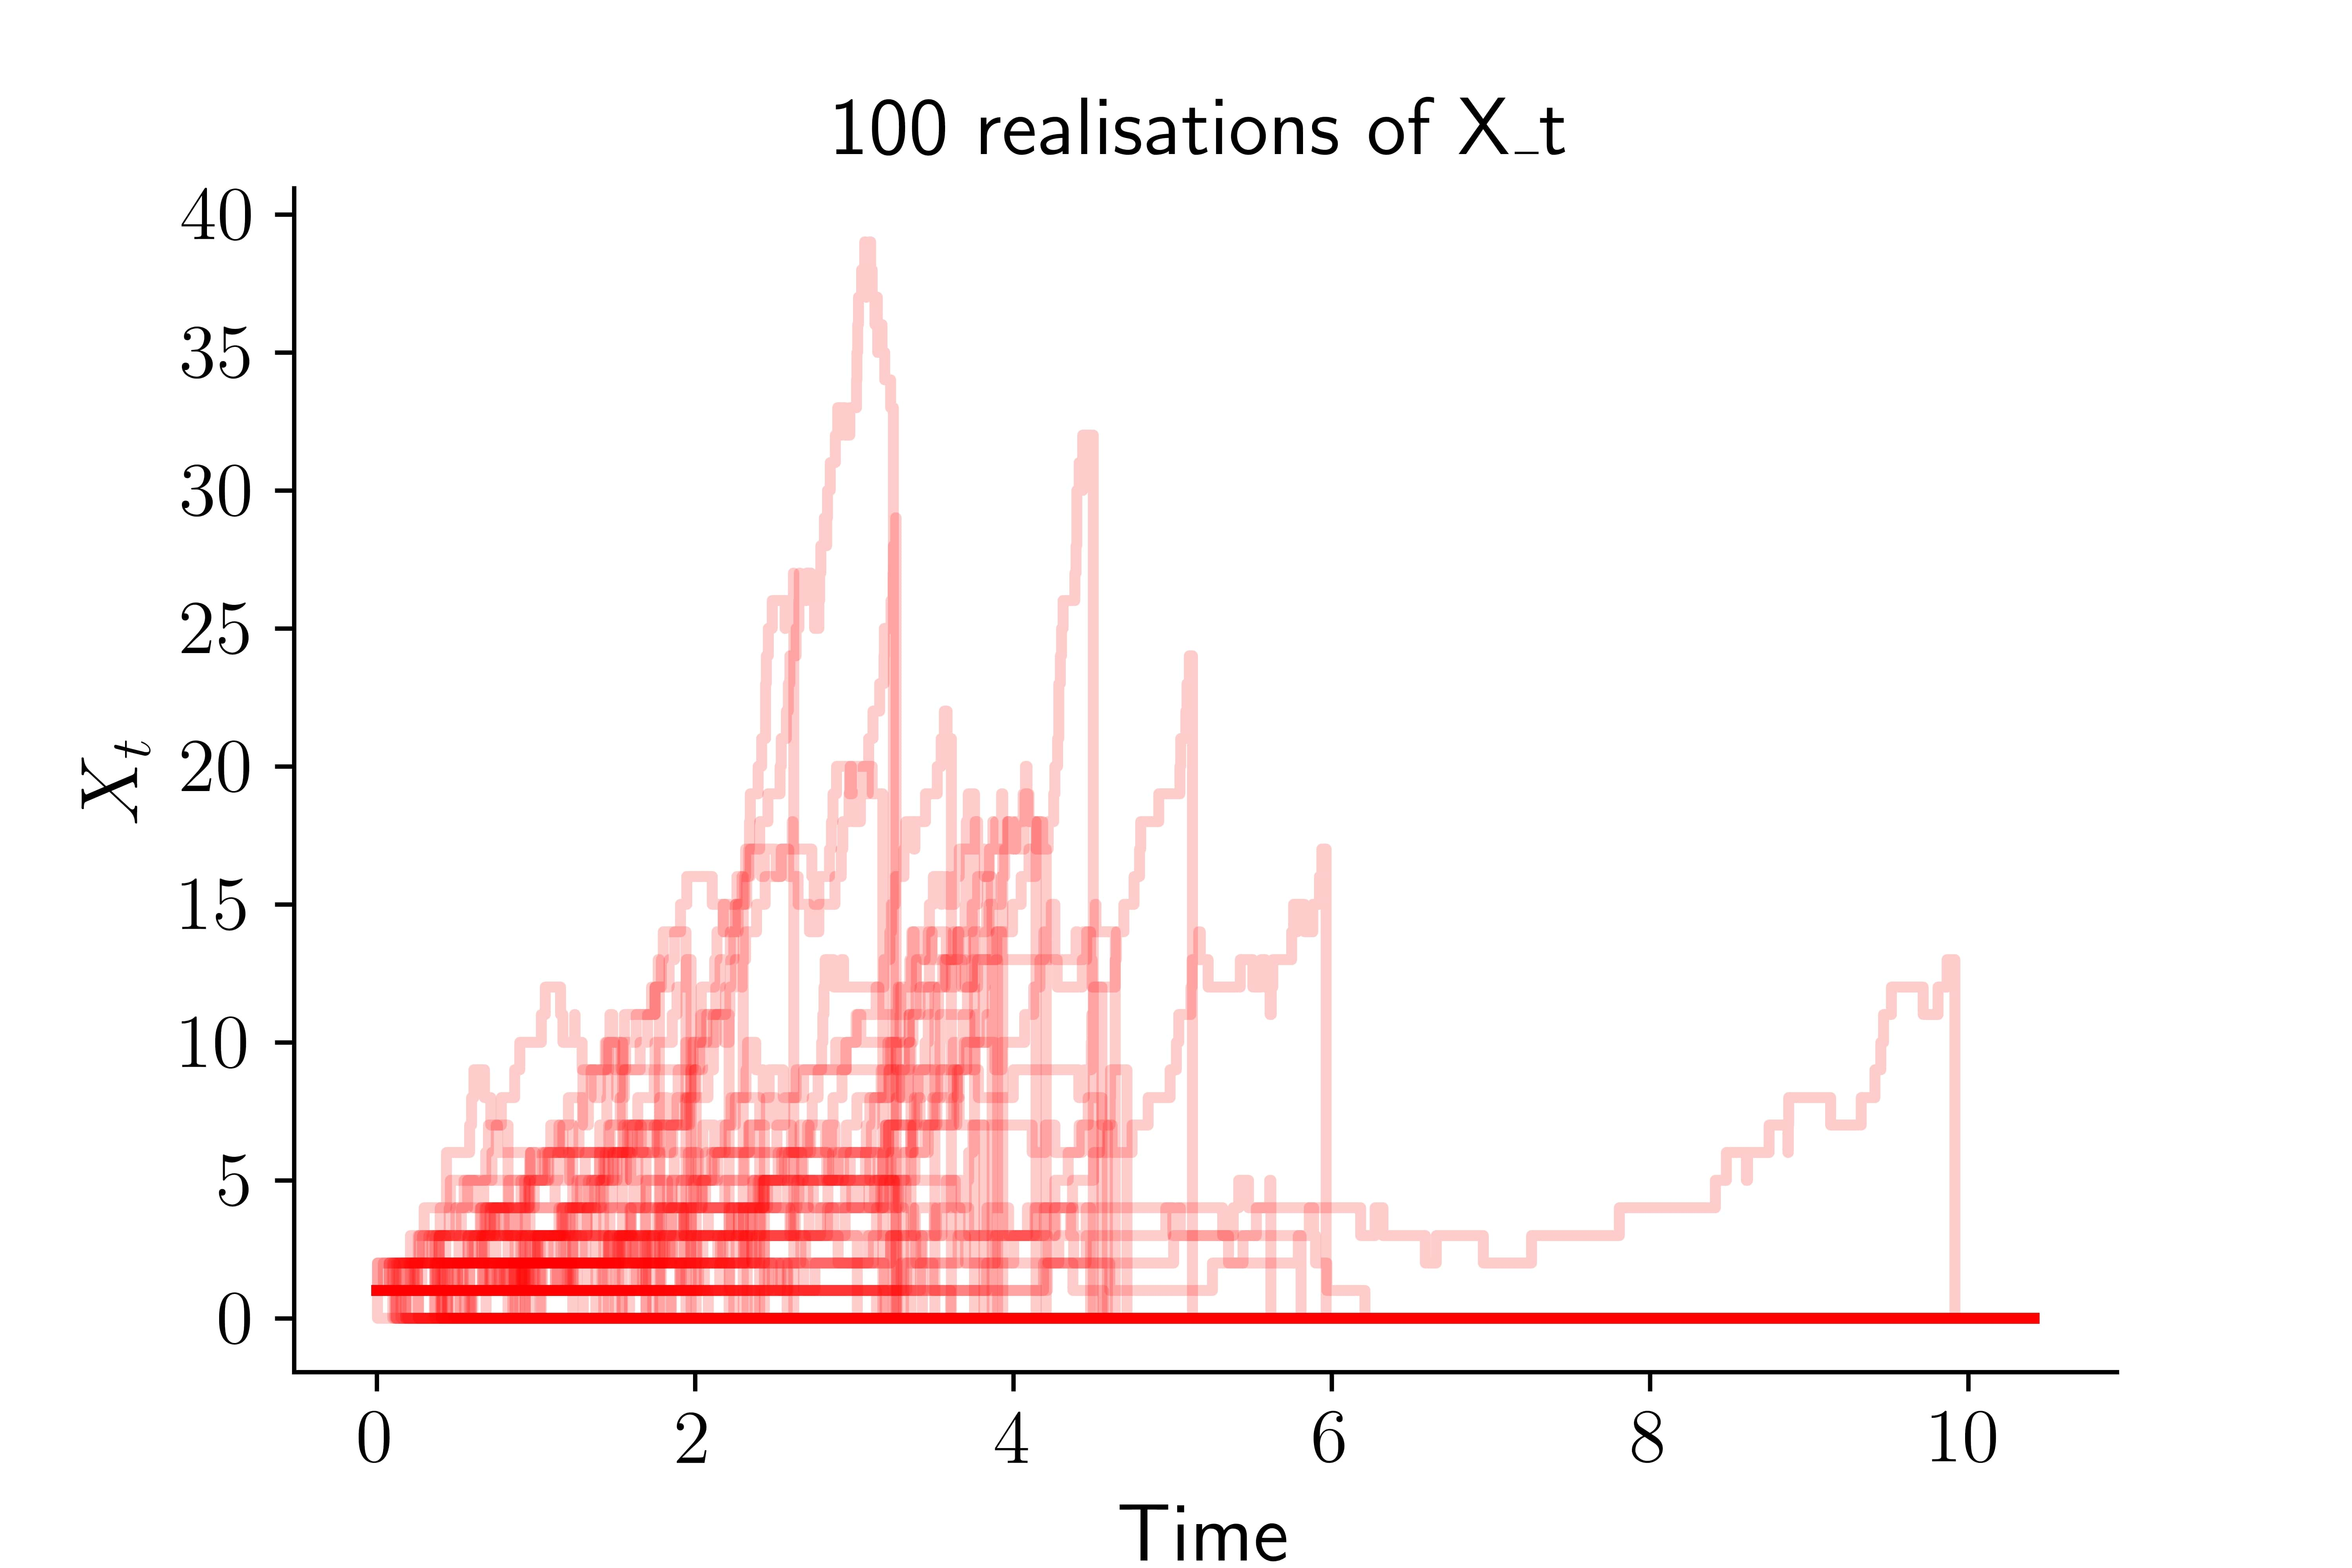
\includegraphics[width = 0.7\textwidth]{chapter4/IMG_ch4/BDRsimulations.jpg}
\caption{100 realisations of $\xt$ generated using the Gillespie algorithm. $\beta = 1$, $\mu = 0$, $\delta = 0.1$. }
\label{BDRsims}
\end{figure}


\subsection*{Choice of rupture state}


An alternative definition lists the ``catastrophe state'' as 0 instead of a $H$. And it would make some intuitive sense to arrange the process like this. After all, following rupture of an infected cell, there are subsequently 0 replicative units within it. But then, it also no longer exists. Ultimately, whether we ascribe the catastrophe state to 0 or $H$ is of no material significance to the dynamics. That is to say, the burst time and sizes observed are unchanged. But there is a distinction created in some of the formulas. These will be mentioned as we continue, but for our purposes, the catastrophe transition will be taken to the isolated state $H$. \par





\subsection*{Post catastrophe count}

For the context we are considering in which the catastrophe signifies the rupture of an infected cell, following this release, some count of infections units will enter the extracellular medium. This post rupture count, assuming no further dynamics, will be fixed by the final value of $\xt$ prior to catastrophe, and it will remain at that value for future time. We will refer to this post rupture count as $\wt$, itself a stochastic process. $\wt = 0$ for $t\leq\tau$, and $\wt = \xx_\tau$ thereafter for $t> \tau$. ($\tau$ being the time of cell rupture).\par
$\wt$ is included in the above definition as follows to describe the full stochastic process, ($\xt$, $\wt$).
\begin{align*}
\pr{\Delta \xt = 1, \Delta \wt = 0} &= \beta \xt \cdot \delt&&\text{(birth)}\\
\pr{\Delta \xt = -1, \Delta \wt = 0} &= \mu \xt  \cdot \delt&&\text{(death)}\\
\pr{\Delta \xt = 0, \Delta \wt = 0} &=1 -  (\beta+\mu+\delta) \xt  \cdot \delt&&\text{(no event)}\\
\pr{\xx_{t+\Delta t} = H, \ww_{t+\Delta t} = \xx_t} &=\delta \xt  \cdot \delt&&\text{(catastrophe)}
\end{align*}
(Using shorthand, $\Delta \xt = \xx_{t+\Delta t}  -  \xt$).


\begin{figure}[H]
\centering
\title{$\wt$}
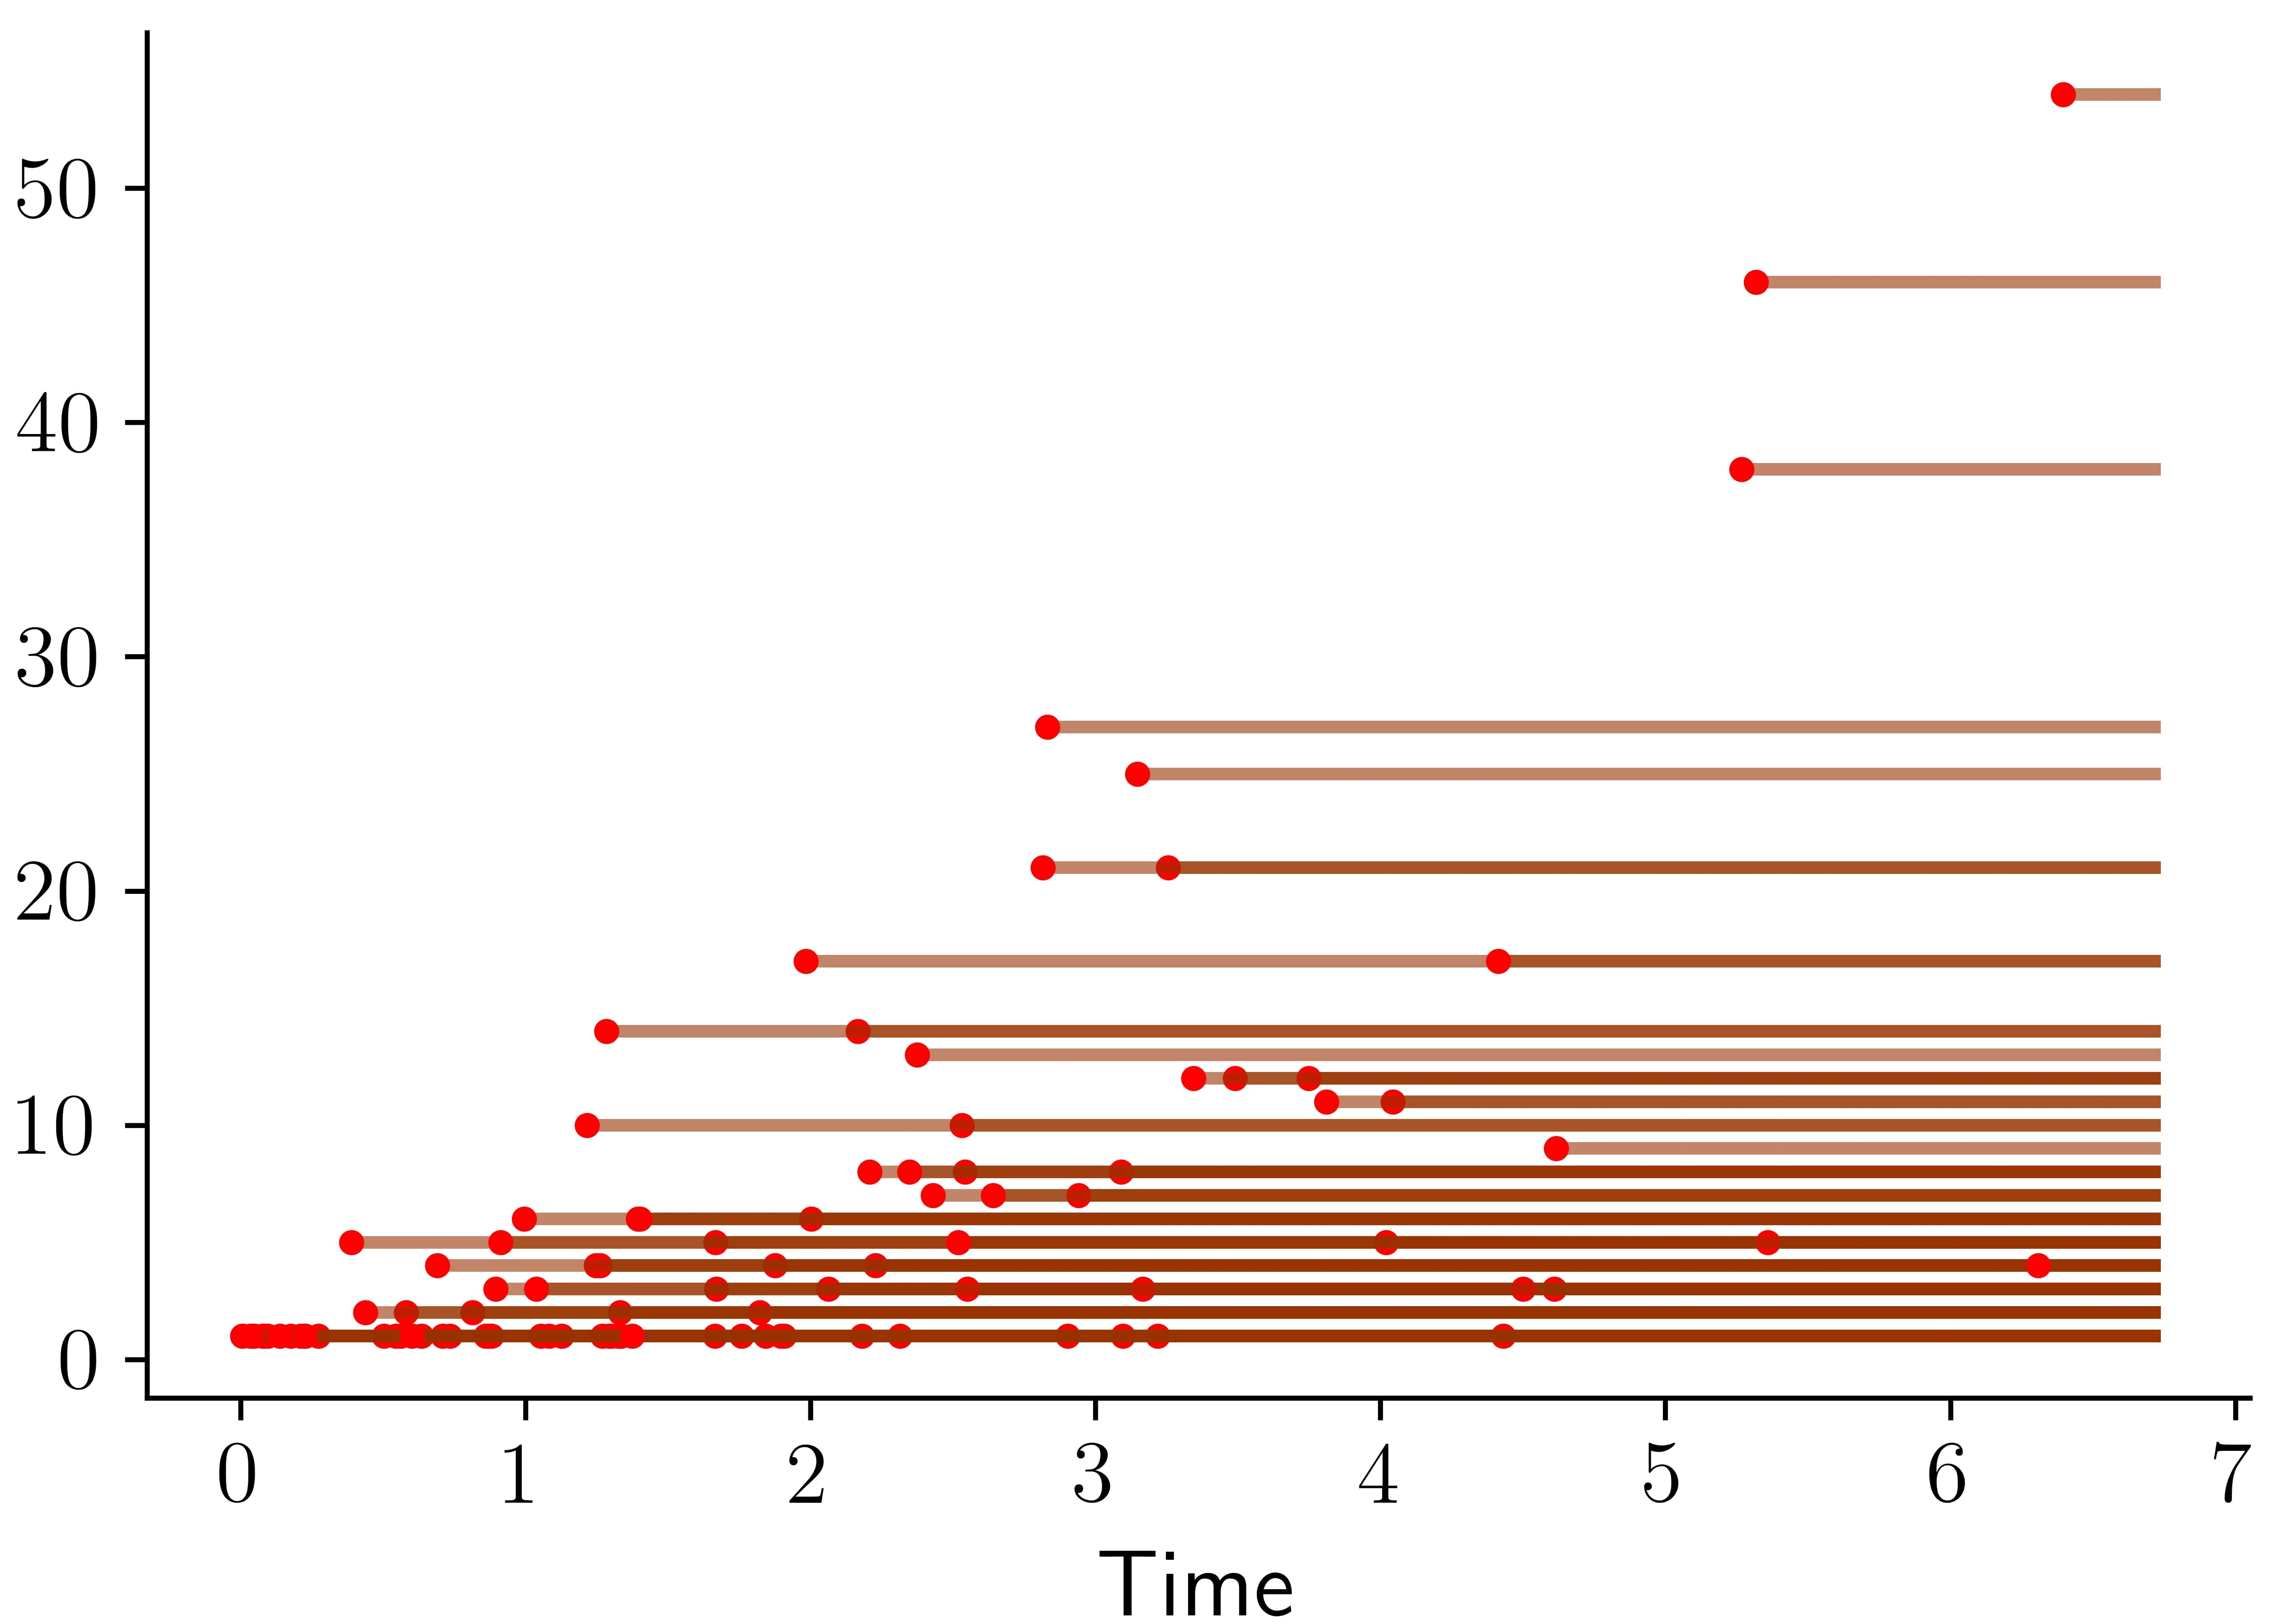
\includegraphics[width = 0.55\textwidth]{chapter4/IMG_ch4/BDRsimulationsY2.jpg}
\caption{100 realisations of $\wt$ generated using the Gillespie algorithm. $\beta = 1$, $\mu = 0$, $\delta = 0.1$. }
\label{BDRsims}
\end{figure}






















%%%%%%%%%%%%%%%%%%%%%%%%%%%%%%%%%%%%%%%%%%%%%%%%%%%%%%%%%%%%%%%%%%%%%%%%%%%%%%%%%%%%%%%%%%%%%%%%%%%%%%%%%%%

\section{Analytical quantities} 








To understand the dynamical properties of the BDC process, there are a handful of quantities for the focus of analysis.  



\subsection*{ ${I(t)}$, the non-catastrophe probability}

\vspace{3pt}
{\Large$$ I(t) = \pr{\xt \neq H|\; \xx_0 = 1}$$
$$\text{ \& }$$
$$\hat I(t) = \pr{\xt \notin \{0, H \}|\; \xx_0 = 1}$$}

\noindent
Given that the rupture state, $H$ is accessible from every non-zero state of the Markov process, eventual catastrophe is inevitable provided the process doesn't fixate by depletion to 0. Hence, either death or catastrophe is sure to happen at late time. $I(t)$ is the probability that the process has not experienced catastrophe prior to time $t$. 

 {\large $$I(t) = \frac{a(1-b) - b(1-a) \ee^{\lambda(a - b)t}}{(1-b) - (1-a) \ee^{\lambda(a - b)t}},$$}
 where 
$$a = \eta+\sqrt{\eta^2-\frac{\mu}{\lambda}}  \qquad  \text{ and } \qquad b =  \eta-\sqrt{\eta^2-\frac{\mu}{\lambda}},$$
with 
$$\eta = \frac{\lambda + \mu + \delta}{2\lambda}$$
This is the solution to a differential equation seen below. When $\mu>0$ and process death is possible.   It will tend down to the positive constant value, $b$, the likelihood of eventual  process death,
 $$\lrb{\lim_{t\to \infty}I(t) = \frac{-b(1-a)}{-(1-a)} = b}$$




\begin{figure}[H]
\xdef\mydelt{0.05}
\xdef\mybeta{1}
\xdef\mymu{0.2}
\begin{center}
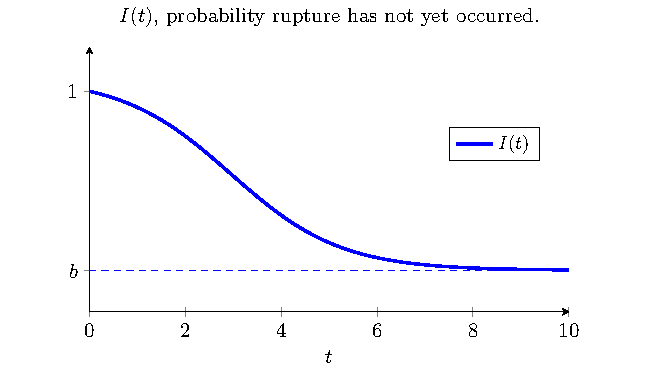
\includegraphics[width = 0.65\textwidth]{chapter4/IMG_ch4/I_of_t_1.pdf}
\end{center}
\caption{$I(t)$ plotted against time. Converges to $I_-$, representing the probability of eventual compartment recovery --- the birth death process dies out before rupture. $\beta=\mybeta$, $\mu=\mymu$, $\delta=\mydelt$}
\end{figure}



We can also consider the non-fixation probability, $\hat I(t)$, signifying the likelihood that at time $t$ the process has neither died, nor experienced catastrophe,
$$\hat I(t) = \pr{\xt \notin \{0, H \}|\; \xx_0 = 1}.$$ 
This will decline asymptotically to 0 signifying the eventual certainty of fixation one way or the other.  The solution is 

$$\hat I(t)  = \frac{2\eta}{1 - (1-2\eta)\ee^{2\eta\lambda t}},$$

$$\lim_{t\to \infty} \hat I(t) = 0.$$
The formulas for both $I(t)$ and $\hat I(t)$ are shown to result from their associated ODEs in the following section. Their form was first established by Kalin and Tavare in the 80s \cite{karlin1982linear}.



\begin{figure}[H]
\xdef\mydelt{0.05}
\xdef\mybeta{1}
\xdef\mymu{0.2}
\begin{center}
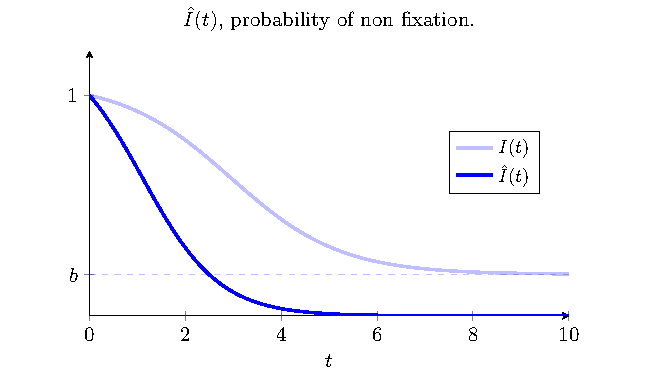
\includegraphics[width = 0.65\textwidth]{chapter4/IMG_ch4/I_of_t_2.pdf}
\end{center}
\caption{$\hat I(t)$ plotted against time. $\beta=\mybeta$, $\mu=\mymu$, $\delta=\mydelt$}
\end{figure}

\noindent
Suppose the process  begins with $k$ initial particles, $\xx_0 = k$. Each replicative unit gives rise to its own set of descendants, all behaving independently from one another. The likelihood through time that any one of those $k$ families will \textit{not} have led to catastrophe is $I(t)$. So it follows naturally, the probability that none of the $k$ families has led to the mass emigration is $\lrbs{I(t)}^k$;
$$  I_k(t) = \pr{\xt \neq H|\; \xx_0 = k} = \lrbs{I(t)}^k.$$
Likewise, when considering fixation more generally, 
$$\hat I_k(t) = \pr{\xt \notin \{0, H \}|\; \xx_0 = k}= \lrbs{\hat I(t)}^k.$$ 
(Is this correct?)










\subsection*{$J(t)$, replicative unit mean}

\vspace{3pt}
{\Large$$J(t) = \mean{\xt|\xx_0 = 1}$$}

\noindent
A given realisation of the process will rise and fall stochastically in steps for some time before ending up stuck either at 0 or, after catastrophe, at $H$. Following each of these fixation outcomes, the contribution of $\xt$ to the mean $J(t)$ is 0. So, supposing we observe 100 realisations, if at time $t=20$ all of them have have either died or undergone catastrophe, their sample mean would be 0 ($J_{\text{sample}}(20) = 0$).


From the initial condition, $\xx_0 = 1$, the process mean will go on to rise with realisations tending to increase, then fall as the likelihood of fixation grows asymptotically certain.

\begin{figure}[H]
\xdef\mydelt{0.05}
\xdef\mybeta{1}
\xdef\mymu{0.2}
\begin{center}
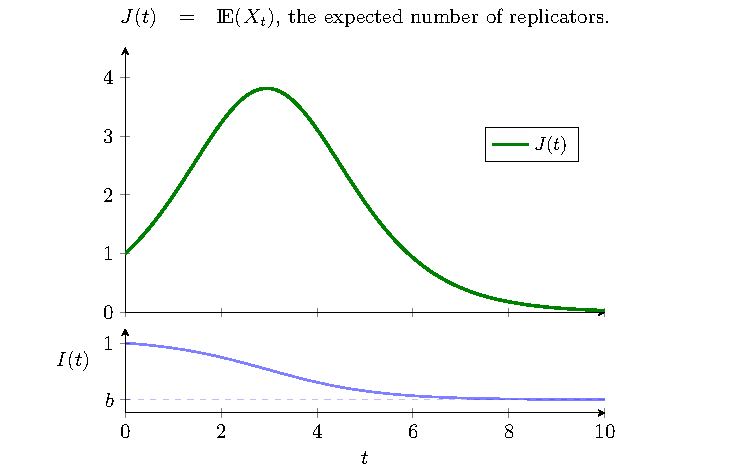
\includegraphics[width = 0.7\textwidth]{chapter4/IMG_ch4/J_of_t_1.pdf}
\end{center}
\caption{$J(t)$ plotted against time. $\beta=\mybeta$, $\mu=\mymu$, $\delta=\mydelt$}
\end{figure}

\noindent
It is given by the formula,

{\large$$J(t) = -\frac{\lambda(1-a)(1-b)(a-b)^2\ee^{\beta(a-b)t}}{\delta\big((1-b) - (1-a)\ee^{\lambda(a-b)t}\big)^2},$$}
which is obtained simply by differentiating $I(t)$ then multiplying by $-\delta^{-1}$. This follows from the equation $I' = -\delta J$ covered in more detail below.












\subsection*{$V(t)$, number of released units}

\vspace{3pt}
{\Large$$V(t) = \mean{\wt| \xx_0 = 1}$$}

\noindent
Over time, the process will either decline to 0, or transition to the catastrophe state, $H$. In which case, $\wt$ will be set at a geometrically distributed quantity seen in the final numeric value of $\xt$. $V(t)$, the expected post rupture count, incorporates all situations, whether $\wt$ is zero or not:

{\large $$V(t) = \frac{(\lambda - \mu)}{\delta}\big[1-I(t)\big] -J(t)+1. $$}
At late time, realisations which ended in both catastrophe, and death will constitute the value of $\lim_{t\to\infty} V(t) = V_{\infty}$.

$$V_{\infty} = \frac{(\lambda - \mu)}{\delta}\big[1-b\big]+1,$$
as $I\to b$ and $J \to 0$; when $\mu = 0$, 
$$V_{\infty} = \frac{\lambda }{\delta}+1.$$

For the case where death is included ($\mu>0$), the formula, $V_{\infty}$, takes into account eventualities in which the process did not attain catastrophe.
We may also extract the mean burst size proper by conditioning for cases which did experienced rupture, effectively discounting the dead realisations. This is done by dividing $V(t)$ by the likelihood of process catastrophe, $1-I(t)$. This is taken from the basic logic,
$$\mean{\wt} = \cancelto{0}{\mean{\wt | \text{no rupture}} I(t) }  + \mean{\wt | \text{rupture}} (1 - I(t)) $$
$$ \mean{\wt | \text{rupture}}  =  \frac{\mean{\wt}}{1 - I(t)},$$
$$\frac{V(t)}{1 - I(t)} $$
represents the expected burst size given catastrophe has taken place by time $t$. The ``overall'' burst size mean is seen in the late time value of this, incorporating all process realisations which experience rupture regardless of when:

\begin{align*}
\mean{\mathcal{K}} = \lim_{t\to \infty} \frac{V(t)}{1 - I(t)} &=  \frac{V_{\infty}}{1 - b} \\
&= \frac{\lambda-\mu}{\delta} + \frac{1}{1-b},
\end{align*}
(recalling that $b$ is the probability of ultimate process death). Notice the alignment $\mean{\mathcal{K}} = V_\infty$ when $\mu=0$. 



PLOT $\mean{\mathcal{K}}$ against $\delta$ for $\mu = 0$, $\lambda = 1$


	
\begin{figure}[H]
\begin{center}

\xdef\mydelt{0.05}
\xdef\mybeta{1}
\xdef\mysum{0.151}
\xdef\mymu{0.2}


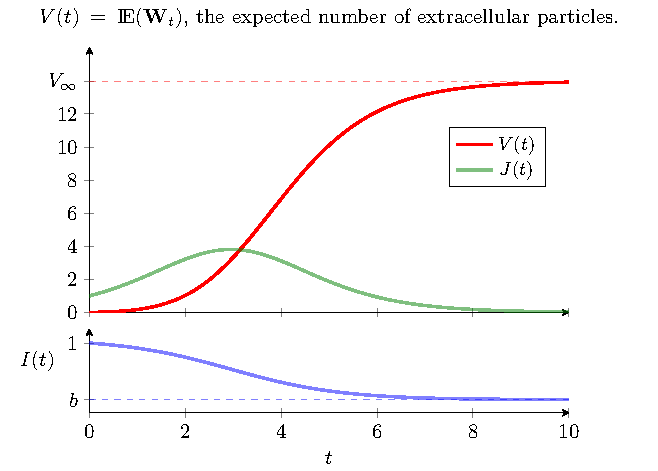
\includegraphics[width = 0.7\textwidth]{chapter4/IMG_ch4/V_of_t_1.pdf}

\end{center}
\caption{$V(t)$ plotted against time. $\beta=\mybeta$, $\mu=\mymu$, $\delta=\mydelt$.}
\end{figure}






\subsection*{$K(t)$, second moment of $\xt$}

\vspace{3pt}
{\Large$$K(t) = \mean{\xt^2| \xx_0 = 1}$$}

\noindent
We became interested in this quantity because it showed up in a term of the ODE describing change in $J(t)$:
$$\ddt{J} = (\lambda - \mu) J - \delta \mean{\xt^2}.$$
This final term results from the following reasoning. With rate $\delta \xt$, the value of $J(t)$ is reduced by $\xt$. So the expected deduction to $\xt$ by catastrophe over an infinitesimal duration is $\mean{ -\delta \xt^2 \delt}$. Hence, in deriving the above ODE, we find the contribution $-\delta \mean{\xt^2}$.




























%%%%%%%%%%%%%%%%%%%%%%%%%%%%%%%%%%%%%%%%%%%%%%%%%%%%%%%%%%%%%%%%%%%%%%%%%%%%%%%%%%%%%%%%%%%%%%%%%%%%%%%%%%%


\section{Derivation of equations and results}


\subsection{First equation}


{\large$$\ddt{I} = \mu - (\lambda + \mu + \delta) I + \lambda I^2$$}



Considering what may happen during an interval of duration $\delt$ after $t=0$, we can write down the equation,
$$I(0+\delt) = \mu \delt + [1 - (\beta + \mu + \delta)\delt] I(0) + \beta\delt {I(0)}^2 + o(\delt). $$
The single initial unit may die, divide, cause rupture, or do nothing at all; each possibility accounted for on the RHS, with the respective event-probabilities multiplied by the updated non-rupture likelihoods --- as if the process were beginning anew. In the case a rupture occurred, this value will obviously be 0; if a birth takes place, it assumes the value, $I_2(0)$. Which, as shown above is equivalent to ${I(0)}^2$. And because the model is homogeneous in time, the relation maintains applicability in subsequent intervals, $[t, t+\delt]$:
$$I(t+\delt) = \mu \delt + [1 - (\beta + \mu + \delta)\delt] I(t) + \beta\delt {I(t)}^2 + o(\delt). $$
Rearranging this yields, 
$$\frac{I(t+\delt) -I(t)}{\delt} = \mu - (\beta + \mu + \delta) I(t) + \beta {I(t)}^2 + \frac{o(\delt)}{\delt}.$$
Which, in the limit as $\delt\to 0$, becomes
\begin{equation}
\label{ddII}
\ddt{I} = \mu - (\beta + \mu + \delta) I + \beta {I}^2,
\end{equation}
a Ricatti equation with solution
\begin{equation}
\label{formI}
I(t) = \frac{I_+(1-I_-) - I_-(1-I_+) \ee^{\beta(I_+ - I_-)t}}{(1-I_-) - (1-I_+) \ee^{\beta(I_+ - I_-)t}}.
\end{equation}
Constants, $I_{\pm}$, given:
\begin{align*}
I_{\pm} = \eta \pm \sqrt{\eta^2 - \frac{\mu}{\beta}}\;, \hspace{20pt} \text{with}\hspace{20pt} \eta = \frac{\beta + \mu + \delta}{2\beta}.
\end{align*}

As an aside, it's worth mentioning that (\ref{ddII}) can be written in in terms of the constants, $I_{\pm}$:

\begin{equation}
\label{ddIIfact}
\ddt{I} =\beta\lrb{I-I_+}\lrb{I-I_+}.
\end{equation}



\noindent
Plotting $\dd I/\dd t$ against $I$ gives an intuitive picture of why $I(t)$ tends to $I_-$ at late time. 


\subsection{Alternative quantity to $I(t)$}
What if we consider the probability that the process has yet to reach the absorbing state of 0 --- by neither rupture, nor the birth-death process dying out? 
$$\hat I(t) = \pr{\xt \neq 0}.$$
When $\mu = 0$, this will be identical to $I(t)$.

The equivalent to equation (\ref{ddII}) is
\begin{equation}
\label{ddIIhat}
\ddt{\hat I} =  -(\beta + \mu + \delta)\hat I + \beta {\hat I}^2,
\end{equation}
as, during its derivation, in the case where the first unit dies, $\hat I(t)$ will become 0 rather than 1, so there is no $\mu$ term on the RHS.

(\ref{ddIIhat}) is solved by
$$\hat I(t) = \frac{\hat\eta}{1 - (1-\hat\eta)\ee^{\hat\eta\beta t}}, $$
with $\hat\eta = (\beta + \mu + \delta)/\beta$.











\section{Expected number of units,  $J(t) = \mean{\xt}$}

Individual realisations of the stochastic process, $\xt$, will vary greatly. When comparing a large number side by side, an increasing count will have collapsed to 0, as those remaining climb higher and higher. (assuming $\beta > \mu$). Despite this, we can quantify the expected (mean) value of the process over time --- call it $J(t)$: 
$$J(t) = \mean{\xt\;|\;\xx_0=1}.$$

\subsection{$J(t)$ as a formula in time}
A formula for $J(t)$ can be obtained with the following line of reasoning. 

Take the forward Kolmogorov equation describing $p_0(t) = \pr{\xt = 0}$.
$$\ddt{p_0} = \delta (1 p_1 + 2 p_2 + 3p_3  + \dots ) + \mu p_1$$
 On the RHS we see a sum of probabilities for the process being in a given state, multiplied by the relevant transition rates to 0. The end term, $\mu p_1$ is associated with death of the final living infectious particle. All of the others relate to catastrophe transitions, from every non-zero state, $i$, and with rates $\delta i$. These conveniently combine and make up the definition of $\mean{\xt}$. So we can write,
$$\ddt{p_0} = \delta J + \mu p_1.$$
Removing the $\mu p_1$ term, we are left with an equation describing the probability that $\xt$  equals $0$, \textit{and} it arrived there following a rupture event --- or, the probability that rupture has occurred. Call it $\hat p_0$. 
$$\ddt{\hat p_0} = \delta J.$$
Since $I(t)$ is the probability rupture has \textit{not} yet happened: $I(t) = 1-\hat p_0$. Hence,
\begin{equation}
\label{ddIJ}
\ddt{I} = -\delta J.
\end{equation}
(\ref{ddIJ}) can be rearranged ---
$$J = -\frac{1}{\delta}\ddt{I}$$
--- and solved for $J(t)$ by differentiating  (\ref{formI}), the formula for $I(t)$:
\begin{equation*}
J(t) = -\frac{\beta(1-I_+)(1-I_-)(I_+-I_-)^2\ee^{\beta(I_+-I_-)t}}{\delta\big((1-I_-) - (1-I_+)\ee^{\beta(I_+-I_-)t}\big)^2}
\end{equation*}







\subsection{Rate of change of $J$}

By looking to the list of possible events over a period $\delt$, we can write down the following relationship describing how $\mean{\xt}$ changes.
$$\mean{\xx_{t+\delt}} = \mean{\xt} + \mean{\xx_{t+\delt}-\xt};$$
the expected value of $\xx_{t+\delt}$ is what it was at time $t$, plus the expected change during the interval [$t$, $t+\delt$].
\begin{equation}
\label{ddJ}
\mean{\xx_{t+\delt}} = \mean{\xt} + \mean{\beta\delt\xt - \mu\delt\xt - \delta\delt\xt\cdot\xt}
\end{equation}
The final compenent, $- \delta\delt\xt\cdot\xt$, represents the probability that a rupture occurs during the interval, $\delta\delt\xt$, multiplied by the change to $\xt$ --- in this case: $-\xt$ (complete elimination).
Rearranging (\ref{ddJ}), we find 
$$\frac{\mean{\xx_{t+\delt}} - \mean{\xt}}{\delt} = \beta\mean{\xt} - \mu\mean{\xt} - \delta \mean{\xt^2}.$$
Which, evaluated in the limit, $\delt \to 0$, becomes
\begin{equation}
\label{ddJ2}
\ddt{J} = (\beta - \mu) J - \delta K(t),
\end{equation}
with
\begin{equation*}
K(t) = \mean{\xt^2}.
\end{equation*}


\subsection{Extracellular count, $V(t)$}

If we define a secondary process, $\yt$, as the number of units ``expelled'' following a rupture event in $\xt$, we can quantify the expected ``extracellular'' particle count through time. To clarify, $\yt$ will remain at 0 unless the associated process $\xt$ undergoes a catastrophe. With probability $1-I_-$, this will happen eventually, in which case $\yt$ will jump from 0 to the value of $\xt$ immediately prior to mass expulsion;
$$\pr{\yy_{t+\delt}-\yt = \xt,\; \xx_{t+\delt}-\xt=0} = \delta\xt\cdot\delt.$$



\noindent
By analogous reasoning that derived (\ref{ddJ2}), it is possible to state
\begin{equation}
\label{ddV}
\ddt{V} =  \delta K(t),
\end{equation}
where $V(t) = \mean{\yt}$.
And this can be solved for $V(t)$ in the following way. (\ref{ddJ2}) and (\ref{ddV}) combine to give,
$$\ddt{J} = (\beta - \mu) J - \ddt{V}.$$
With (\ref{ddIJ}), this can be rearranged into,
$$\ddt{V} = -\frac{(\beta - \mu)}{\delta}\ddt{I} - \ddt{J}.$$ 
Then, integrating:
$$V(t) = -\frac{(\beta - \mu)}{\delta}I(t) - J(t) + \text{const}.$$
And finally with initial conditions, $V(0) = 0$, and $J(0)=I(0)=1$,
\begin{equation*}
\label{Voft}
V(t) = \frac{(\beta - \mu)}{\delta}\big[1-I(t)\big] -J(t)+1.
\end{equation*}




\noindent
In late time, $V(t)$ will tend to
$$V_{\infty} =  \frac{(\beta - \mu)}{\delta}\big[1-I_-\big] +1,$$
which can be interpreted as the expected rupture size. 

When $\mu = 0$,
$$V_\infty = 1 +\frac{\beta}{\delta}.$$





\section{Variance and standard deviation of $\xt$ \& $\yt$}

To describe the variance of a random variable, it is standard to use the formula, 
\begin{equation*}
\text{Var}(\xt) = \mean{\xt^2} - \mean{\xt}^2.
\end{equation*}
And we can apply this to $\xt$ and $\yt$ to quantify the variability of intracellular and extracellular particles as functions of time. 

In each case, we will first require a formula for the expected value of the counts squared,  $\mean{\xt^2}$ and $\mean{\yt^2}$.






\subsection{Variance of $\xt$}

\subsubsection{Formula for $\mean{\xt^2}$ ($ = K(t)$)}

A formula for $K(t) = \mean{\xt^2}$ is derived in the following way. Taking the time derivative of equations,

 (\ref{ddIJ}): ${\rm d}I/{\rm d}t = -\delta J$, and, 
 
 (\ref{ddII}): ${\rm d}I/{\rm d}t = \mu - (\beta + \mu + \delta) I + \beta I^2$.

\begin{align}
\label{Kderev1}
\text{(\ref{ddIJ})}\to&&\ddt{J} = -\frac{1}{\delta}\frac{\dd^2 I}{\dd t^2}&&
\end{align}
\begin{align*}
\text{(\ref{ddII})}\to&& \frac{\dd^2 I}{\dd t^2} = -(\beta + \mu + \delta) \ddt{I} + 2\beta I \ddt{I}.&&
\end{align*}
The latter, with ${\rm d}I/{\rm d}t = -\delta J$, becomes
\begin{equation}
\label{Kderev2}
\frac{\dd^2 I}{\dd t^2} = (\beta + \mu + \delta)\beta J- 2\beta \delta I J.
\end{equation}
Comparing (\ref{Kderev2}) with (\ref{Kderev1}),
\begin{equation*}
%\label{Kderev3}
\ddt{J} = -(\beta + \mu + \delta) J + 2\beta I J;
\end{equation*}
then, this with (\ref{ddJ2}),
$$(\beta - \mu) J - \delta K = -(\beta + \mu + \delta) J + 2\beta I J.$$
Rearranging for $K(t)$,
\begin{equation}
\label{Kt1}
K(t) = \frac{2\beta}{\delta}\lrb{1+\frac{\delta}{2\beta} - I}J.
\end{equation}
Considering (\ref{ddIIfact}) and (\ref{ddIJ}), this may also be written as
\begin{equation}
\label{KtI}
K(I) = -\frac{2\beta^2}{\delta}\lrb{I-\kappa}\lrb{I-I_-}\lrb{I-I_+}.
\end{equation}
with,
$$\kappa = 1+\frac{\delta}{2\beta}.$$



\subsubsection{One standard deviation from the mean, $J(t)$}
With the expectation of $\xt^2$, (\ref{Kt1}), 
\begin{equation*}
K(t) = \frac{2\beta}{\delta}\lrb{\kappa- I}J,
\end{equation*}
we can write down the variance of $\xt$ using $\text{Var}(\xt) = \mean{\xt^2} - \mean{\xt}^2$:
\begin{align*}
\text{Var}(\xt) &= K(t) - {J(t)}^2\\
&= \frac{2\beta}{\delta}\lrb{\kappa - I}J - J^2.
\end{align*}
The standard deviation is then,
\begin{equation*}
\text{Std}(\xt) = \sqrt{\frac{2\beta}{\delta}\lrb{\kappa- I}J - J^2}.
\end{equation*}



\subsection{Variance of $\yt$}

We can likewise compute the variance of $\yt$ using $\text{Var}(\yt) = \mean{\yt^2} - \mean{\yt}^2$. To begin, we must find a formula for $\mean{\yt^2}$.


\subsubsection{Formula for $\mean{\yt^2}$}


Accounting for changes to $\yt^2$ over an infinitesimal time $\delt$,
$$\mean{\yy_{t+\delt}^2} = \mean{\yt^2} + \mean{\yy_{t+\delt}^2 - \yt^2},$$
we can derive the equation
\begin{equation}
\label{meanYt2}
\ddt{\mean{\yt^2}} = \delta \mean{\xt^3}.
\end{equation}
This might seem like a dead end as we have yet do come up with a description of $\mean{\xt^3}$. Though as it happens, the problem can be sidestepped by thinking about the rate of change of $K(t) = \mean{\xt^2}$. An equation for $\dd K/\dd t$ can be derived as follows. 
\begin{equation}
\label{meanysq1}
\mean{\xx_{t+\delt}^2} = \mean{\xt^2} + \mean{\xx_{t+\delt}^2 - \xt^2}
\end{equation}
Because of the quadratic, changes in $\xt^2$ require special attention (see table).
\begin{table}[ht]
\centering
\renewcommand{\arraystretch}{1.5} % Increase vertical padding
\setlength{\tabcolsep}{17pt} % Increase horizontal padding
\begin{tabular}{|>{\centering\arraybackslash}m{3cm}|>{\centering\arraybackslash}m{2cm}|>{\centering\arraybackslash}m{5cm}|}
\hline
Probability of occurrence& Change in $\xt$ & Change in $\xt^2$\\
\hline
\hline
$\beta \xt\delt$& 1 & $(\xt + 1)^2 - \xt^2 = 2\xt + 1$ \\
\hline
$\mu \xt\delt$ &-1 & $(\xt - 1)^2 - \xt^2 = -2\xt + 1$\\
\hline
$\delta \xt\delt$ & $-\xt$& $(\xt - \xt)^2 - \xt^2 = -\xt^2$ \\
\hline
\end{tabular}
\end{table}

\noindent
From the possibilities, it can be seen that
\begin{align*}\mean{\xx_{t+\delt}^2 - \xt^2} &={\rm I}\!{\rm E}\bigg[\beta \xt\delt\cdot(2\xt+1) + \mu \xt\delt\cdot(-2\xt+1) + \delta \xt\delt\cdot(-\xt)\bigg]\\
&=\bigg[ 2(\beta-\mu)\mean{\xt^2} + (\beta+\mu)\mean{\xt} - \delta\mean{\xt^3} \bigg]\delt
\end{align*}
Taking this with (\ref{meanysq1}), the following equation can be obtained in the $\downarrow \delt$ limit.
$$\ddt{\mean{\xt^2}} = 2(\beta-\mu)\mean{\xt^2} + (\beta + \mu)\mean{\xt} - \delta\mean{\xt^3};$$
it can also be written,
\begin{equation}
\label{ddK2}
\ddt{K} =2(\beta-\mu)K+ (\beta + \mu)J- \delta\mean{\xt^3}.
\end{equation}
With this, and equation (\ref{meanYt2}), we will see that it is possible to derive a formula for $\mean{\yt^2}$. 

Substituting into (\ref{ddK2}) with (\ref{meanYt2}), 
$$\ddt{K} =2(\beta-\mu)K+ (\beta + \mu)J- \ddt{\mean{\yt^2}}.$$
Then, using $J = \delta^{-1}\dd I/\dd t$ (\ref{ddIJ}), and $K = \delta^{-1} \dd V / \dd t$ (\ref{ddV}):
\begin{equation}
\ddt{\mean{\yt^2}} = 2\frac{(\beta-\mu)}{\delta}\ddt{V}+ \frac{(\beta + \mu)}{\delta}\ddt{I} - \ddt{K}.
\end{equation}
Which, with the initial conditions, $(I(0), K(0), V(0), \mean{\yy_0^2}) = (1,0,0,0)$, provides $\mean{\yt^2}$ by integration:
\begin{equation}
\label{meanEY2}
\mean{\yt^2} = 2\frac{\beta-\mu}{\delta} V + \frac{\beta+\mu}{\delta}I + K - \frac{\beta+\mu}{\delta}
\end{equation}


\subsubsection{One standard deviation from the mean, $V(t)$}

Using (\ref{meanEY2}), it is possible to write down a formula for the variance of $\yt$,
\begin{equation}
\label{VarY}
\text{Var}(\yt) = 2\frac{\beta-\mu}{\delta} V + \frac{\beta+\mu}{\delta}I + K - \frac{\beta+\mu}{\delta} - V^2
\end{equation}


























\section{Variable dependencies on $I(t)$}

It happens to be possible to write all of the formulas, $J(t)$, $\text{Var}(\xt)$, $V(t)$, $\text{Var}(\yt)$, as functions of the non-rupture probability $I(t)$. 


\subsection{Mean and variance of $\xt$}

Since $J = \delta^{-1}{\dd I}/{\dd t} $, and ${\dd I}/{\dd t} =  \beta (I - I_+)(I-I_-)$ (from (\ref{ddIJ})), we can write $J$ in terms of $I$:
\begin{equation}
\label{JI}
J(I) = -\frac{\beta}{\delta}  (I - I_+)(I-I_-).
\end{equation}
Combining this with (\ref{KtI}), we can also write $\text{Var}(\xt)$ as a function of $I(t)$,

\begin{align*}
\text{Var}(\xt) &= K(I) - {J(I)}^2\\
&=-\frac{2\beta^2}{\delta}\lrb{I-\kappa}\lrb{I-I_-}\lrb{I-I_+} - \lrb{\frac{\beta}{\delta}  (I - I_+)(I-I_-)}^2,
\end{align*}
$$\lrb{\kappa = 1+\frac{\delta}{2\beta}}.$$



\subsection{Mean and variance of $\yt$}

As we have defined $V(t)$ in terms of $I(t)$ and $J(t)$, it is likewise possible to use (\ref{JI}) to write $V(I)$, a function only of the non-rupture probability:
$$V(I) = \frac{\beta - \mu}{\delta}\lrb{1-I} + \frac{\beta}{\delta} (I - I_+)(I-I_-) + 1.$$
And given (\ref{VarY}), we can do the same for the variance of $\yt$:
$$\text{Var}(\yt) = 2\frac{\beta-\mu}{\delta} V(I) + \frac{\beta+\mu}{\delta}I + K(I) - \frac{\beta+\mu}{\delta} - {V(I)}^2;$$


\begin{multline*}
\text{Var}(\yt) = 2\frac{\beta - \mu}{\delta} \lrbs{ \frac{\beta - \mu}{\delta}\lrb{1-I} + \frac{\beta}{\delta} (I - I_+)(I-I_-) + 1} + \\
\frac{\beta+\mu}{\delta} I -\frac{2\beta^2}{\delta}\lrb{I-\kappa}\lrb{I-I_-}\lrb{I-I_+} - \frac{\beta + \mu}{\delta} - \\ \lrbs{\frac{\beta - \mu}{\delta}\lrb{1-I} + \frac{\beta}{\delta} (I - I_+)(I-I_-) + 1}^2.
\end{multline*}




































\section{Variance and standard deviation of $\xt$ \& $\yt$}

To describe the variance of a random variable, it is standard to use the formula, 
\begin{equation*}
\text{Var}(\xt) = \mean{\xt^2} - \mean{\xt}^2.
\end{equation*}
And we can apply this to $\xt$ and $\yt$ to quantify the variability of intracellular and extracellular particles as functions of time. 

In each case, we will first require a formula for the expected value of the counts squared,  $\mean{\xt^2}$ and $\mean{\yt^2}$.
These will be computed first.





\subsection{Variance of $\xt$}

\subsubsection{Formula for $\mean{\xt^2} = K(t)$}

$K(t) = \mean{\xt^2}$ is derived in the following way. Taking the time derivative of equations,

 (\ref{ddIJ}): ${\rm d}I/{\rm d}t = -\delta J$, and, 
 
 (\ref{ddII}): ${\rm d}I/{\rm d}t = \mu - (\beta + \mu + \delta) I + \beta I^2$.

\begin{align}
\label{Kderev1}
\text{(\ref{ddIJ})}\to&&\ddt{J} = -\frac{1}{\delta}\frac{\dd^2 I}{\dd t^2}&&
\end{align}
\begin{align*}
\text{(\ref{ddII})}\to&& \frac{\dd^2 I}{\dd t^2} = -(\beta + \mu + \delta) \ddt{I} + 2\beta I \ddt{I}.&&
\end{align*}
The latter, with ${\rm d}I/{\rm d}t = -\delta J$, becomes
\begin{equation}
\label{Kderev2}
\frac{\dd^2 I}{\dd t^2} = (\beta + \mu + \delta)\beta J- 2\beta \delta I J.
\end{equation}
Comparing (\ref{Kderev2}) with (\ref{Kderev1}),
\begin{equation*}
%\label{Kderev3}
\ddt{J} = -(\beta + \mu + \delta) J + 2\beta I J;
\end{equation*}
then, this with (\ref{ddJ2}),
$$(\beta - \mu) J - \delta K = -(\beta + \mu + \delta) J + 2\beta I J.$$
Rearranging for $K(t)$,
\begin{equation*}
K(t) = \frac{2\beta}{\delta}\lrb{1+\frac{\delta}{2\beta} - I}J
\end{equation*}



\subsubsection{One standard deviation from the mean, $J(t)$}
With the expectation of $\xt^2$,
\begin{equation*}
K(t) = \frac{2\beta}{\delta}\lrb{\kappa- I}J
\end{equation*}
$$\bigg( \kappa = 1+\frac{\delta}{2\beta}\bigg),$$
we can write down the variance of $\xt$ as,
\begin{align*}
\text{Var}(\xt) &= K(t) - {J(t)}^2\\
&= \frac{2\beta}{\delta}\lrb{\kappa - I}J - J^2.
\end{align*}
The standard deviation is then,
\begin{equation*}
\text{Std}(\xt) = \sqrt{\frac{2\beta}{\delta}\lrb{\kappa- I}J - J^2}.
\end{equation*}
























\section{Variable dependencies on $I(t)$}


\subsection{$J(I)$}

Since $J = \delta^{-1}{\dd I}/{\dd t} $, and ${\dd I}/{\dd t} =  \beta (I - I_+)(I-I_-)$ (from (\ref{ddIJ})), we can write $J$ in terms of $I$:

\begin{equation*}
J(I) = -\frac{\beta}{\delta}  (I - I_+)(I-I_-).
\end{equation*}


\subsection{$V(I)$}


Given this, $K$ can also be written as a function of $I$:
\begin{equation*}
K(I) = \frac{2\beta^2}{\delta^2}(I-k)(I - I_+)(I-I_-).
\end{equation*}
labelling $k = 1+ \delta/2\beta$. The same follows for $V$, and $\text{Var}(\xt)$:
\begin{equation*}
V(I) = \frac{\beta - \mu}{\delta}\lrbs{1-I} - J(I) + 1
\end{equation*}
\begin{equation*}
\text{Var}(\xt) = K(I) - J(I)^2
\end{equation*}









\chapter{Birth death catastrophe -- further results and potential use} 





















\section{Specification of rupture state}
Before we begin, it is important to state a distinction between two varieties of the Birth Death Killing model.
When a rupture event occurrs, the process goes to a state. In the literature, this state is sometimes chosen to be 0, and in other cases there is a seperate rupture state defined, sometimes labeled $R$. The analysis does differ between the two options. And so for clarity, in this document we will refer to the 0 state case as ``killng''; the distinct rupture state as ``catastrophe''.  

\section{Probability Generating Function PDEs}
The probability generating function (PDF),  is defned:
$$G(z,t) = p_0(t) + p_1(t)z + p_2(t)z^2 + p_3(t)z^3 + \dots.$$
The following ODEs can be derivd from the forward Kolmogorov associated with the two processes.

\subsubsection*{Catastrophe}

\begin{equation}
\label{catEq1}
\pdx{G(z,t)}{t} = \big(\beta z^2 - (\beta + \mu + \delta)z + \mu\big)\pdx{G}{z}
\end{equation}

\subsubsection*{Killing}

\begin{equation}
\pdx{G(z,t)}{t} = \delta J(t) +  \big(\beta z^2 - (\beta + \mu + \delta)z + \mu\big)\pdx{G}{z}
\label{killEq1}
\end{equation}

\subsubsection*{Derivation}

It will be sufficient to show a derivation of the ``killing'' equation. The ``catastrophe'' version is similar and simpler. \par

Take the forward Kolmogorov equations: 

$$\begin{cases}
    \ddt{p_i} = \beta (i-1) p_{i-1} + \mu (i+1) p_{i+1} - (\beta + \mu + \delta)ip_i, & i > 0\\
   \\
    \ddt{p_0} = \mu p_1 +  \delta\sum^\infty_{j=1} jp_j.
\end{cases}$$
($p_i = \pr{\xt = i}$, probability the process is in state $i$). In the latter equation with $p_0$, the summation represents all of the possible rupture transitions; from any other state, a collapse to 0 can take place. This summation happens to express the mean; $\mean{\xt}$, which is elsewhere labelled $J(t)$.\par 
In the catastrophe version, since rupture causes transition to a separate state, this summation term is not present, and the first equation will be valid for all $i$.\par
\vspace{10pt}

\noindent
A derivation can be executed by manipulating the equations to fabricate terms containing the PGF, $G(z, t) = \sum^\infty_{i=0}p_i z^i$. It begins by multiplying each side of every $i$th equality by $z^i$. In the case of $i=0$, $z^0 = 1$, so there is no change. 


$$\begin{cases}
    \ddt{p_iz^i} = \beta (i-1) p_{i-1}z^i + \mu (i+1) p_{i+1}z^i - (\beta + \mu + \delta)ip_iz^i, & i > 0\\
   \\
    \ddt{p_0} = \mu p_1 +  \delta J(t).
\end{cases}$$

\noindent
Then, each equation is combined in a sum over all values of $i$ for which there is a positive term.

$$
\sum^\infty_{i=0} \pdx{p_iz^i}{t} = \delta J(t)   + \sum^\infty_{i=0}\lrbs{ \beta (i-1) p_{i-1}z^i + \mu (i+1) p_{i+1}z^i - (\beta + \mu + \delta)ip_iz^i}$$

\noindent
Some rearrangement converts this into 

$$\pdx{}{t}{\sum^\infty_{i=0} p_iz^i } = \delta J(t) + \beta z^2 \sum^\infty_{i=1} ip_iz^{i-1} + \mu\sum^\infty_{i=1}ip_iz^{i-1} - (\beta +\mu+\delta)z\sum^\infty_{i=1}ip_iz^{i-1}$$

\noindent
And since
$$\sum^\infty_{i=1} ip_iz^{i-1}  = \pdx{}{z}\sum^\infty_{i=1} p_iz^{i} = \pdx{G(z,t)}{z},$$
the above, becomes 

$$\pdx{G(z,t)}{t} = \delta J(t) +  \beta z^2\pdx{G}{z}  + \mu\pdx{G}{z} - (\beta + \mu + \delta)z\pdx{G}{z}.$$

\noindent
Equivalent to (\ref{killEq1}).

\section{Identifying the PGFs}

G(z,t), the probability generating function, is a powerful tool for understanding the behaviour of the system and its probable outcomes. Because it can be written as a polynomial sum in which each coefficient is the probability of the process being in a specific state at a given time, valuable information on the process can be extracted. \par
As,
$$G(z,t) = p_0(t) + p_1(t)z + p_2(t)z^2 + p_3(t)z^3 + \dots,$$
The mean, $J(t)$ can be found with $\partial_zG(z,t)|_{z=1}$:
$$\mean{\xt} = p_1(t) + 2p_2(t) + 3p_3(t) + \dots;$$
Individual state-probabilities can be extracted in the following way. Differentiate with respect to $z$, $n$ times,
$$\pdxn{G(z,t)}{z}{n} =  n! \cdot p_n(t) + (n+1)! \cdot p_{n+1}(t) z + \frac{(n+2)!}{2} \cdot p_{n+2}(t) z^2 + \dots,$$
then evaluate at $z=0$ and divide by $n!$:
\begin{equation}
\label{stateFormula}
\frac{1}{n!}\cdot\pdxn{G(z,t)}{z}{n}\bigg|_{z=0} = p_n(t).
\end{equation}
In this way the full dynamic distribution of the system can be elucidated.

Though to do this, we must first obtain the explicit formula $G(z,t)$. There will be some difference between the two cases, but the process is similar --- both (\ref{catEq1}) and (\ref{killEq1}) can be solved with the method of characteristics. 


\subsection{Method of characteristics}

Generally, first order, linear PDEs of the type we are dealing can be solved as a family of ODEs. The method begins by introducing a change of variables $(z,t)\to(s,\tau)$;
$$G(z,t)\equiv G\lrb{z(s, \tau),t(s,\tau)} = G(s, \tau).$$
It proceeds by seeking solutions on characteristic lines of constant $s$: $G(\tau)$. An initial curve must be fixed, from which these solutions will progress. The selection is somewhat arbitrary; many options will work, though a good choice can keep the analysis more simple. There are some hard conditions. For example, the initial line must not be parallel in the $s,$ $\tau$ space to the progressing solutions. In cases such as ours, it is often appropriate to use
\begin{align}
\label{ICs}
z(s,0) = s&& t(s,0) = 0
\end{align}
\subsubsection*{Catastrophe}
Assuming the probability generating function changes with only  one variable --- $G(\tau(z, t))$ --- we can write down the characteristic equations as ODEs. First, consider
\begin{equation*}
\dda{G}{\tau} =  \lrbc{\dda{t}{\tau}}  \pdx{G}{t}+ \lrbc{\dda{z}{\tau} }\pdx{G}{z}.
\end{equation*}
Comparing with the catastrophe equation, (\ref{catEq1}), there is a similarity,
$$0=  \lrbc{- 1}\pdx{G}{t} + \lrbc{\beta z^2 -( \beta + \mu + \delta)z + \mu} \pdx{G}{z},$$
and we can extract the three characteristic ODEs:
\begin{align*}
\label{Char1}
\dda{G}{\tau} = 0,&& \dda{t}{\tau} = -1, && \dda{z}{\tau} = \beta z^2 - (\beta + \mu + \delta)z + \mu.
\end{align*}
The first of these, which will differ in the killing case, tells us that  
$$G = \phi{(s)},$$
$\phi$ constant on curves of unchanging $s$.\par
In both cases, the initial condition on $G$ will be $$G(z, 0) = z$$ because starting with a single individual means $p_1(0) =1$ and $p_{i\neq1}(0) = 0$. Therefore, $G = \phi{(s)}$ in conjunction with our choice of initial curve, $z(s, 0) = s$, allows $\phi(s)$ to be fixed as $s$;
$$G(s,\tau) = s.$$\par

\noindent
Moving to the second characteristic ODE:
$$\dda{t}{\tau} = -1 \hspace{5pt} \implies \hspace{5pt} t = -\tau +  C_1(s) \text{  (constant for unchanging }s ).$$
Our initial condition, $t(s,0) = 0$ fixes $C_1(s) = 0$, so $t = -\tau$.\par
The remaining characteristic equation with $z$ happens to be the same form as an ODE describing the no-rupture probability, $I(t)$. 
\begin{equation}
\label{char3cat}
\dda{z}{\tau} = \beta z^2 - (\beta + \mu + \delta)z + \mu
\end{equation}
What differs is the initial condition. In the case of, $I(t)$, at time 0 it is 1 --- rupture having definitely not occurred; with $z(s,t)$, our chosen initial condition is $z(s, 0) = s$. Hence, the solution to (\ref{char3cat}) is very similar to the formula for $I(t)$, though in places where there is seen a one, here an $s$ is found:
\begin{equation*}
z = \frac{a(s-b) - b(s-a)\ee^{\beta(a-b) \tau} } {(s-b) - (s-a)\ee^{\beta(a-b) \tau}}
\end{equation*}
also, In this it is $\tau$ rather than $t$.\par
Since $G(z, t) = s(z, t)$, we can obtain the final solution in one step: Rearrange the above for $s$, and place $-t$ at each $\tau$. By a happenstance of symmetry, this turns out looking quite the same:
\begin{equation}
\label{s2343}
s = \frac{a(z-b) - b(z-a)\ee^{\beta(a-b) t} } {(z-b) - (z-a)\ee^{\beta(a-b) t}}.
\end{equation}
And so we have it, by the somewhat dark art of characteristics, the probability generating function emerges as
\begin{equation*}
G(z,t) = \frac{a(z-b) - b(z-a)\ee^{\beta(a-b) t} } {(z-b) - (z-a)\ee^{\beta(a-b) t}}.
\end{equation*}
As will be seen, in obtaining the state probabilities via repeated partial differentiation in $z$, it is advantageous to write the formula as
\begin{equation*}
G(z,t) = \frac{ab(1-\ee^{\beta(a-b) t}) - z(a-b\ee^{\beta(a-b) t}) } {  (b-a\ee^{\beta(a-b) t}) -z(1-\ee^{\beta(a-b) t})  }
\end{equation*}
For now, let us move on to the modification that is introduced in the killing case. 


\subsubsection*{Killing}

When rupture collapses the process to 0, it may have happened at any positive state.  As we've seen, because of this, the forward Kolmogorov equation describing $p_0(t)$ includes a separate term related to every natural number. Thankfully, these do compress neatly into an expression of the mean, $\mean{\xt} = J(t)$. Hence, in the PDE, (\ref{killEq1}), there is an inhomogeneous term: $\delta J(t)$.\par
Making the same comparison as in the catastrophe case, 

\begin{align*}
\dda{G}{\tau} &=  \lrbc{\dda{t}{\tau}}  \pdx{G}{t}+ \lrbc{\dda{z}{\tau} }\pdx{G}{z}\\
-\delta J(t)&=  \lrbc{- 1}\pdx{G}{t} + \lrbc{\beta z^2 -( \beta + \mu + \delta)z + \mu} \pdx{G}{z}
\end{align*}
we see the characteristic equations are largely the same, just that the first picks up this extra component: 
\begin{align*}
\label{Char2}
\dda{G}{\tau} = -\delta J(-\tau),&& \dda{t}{\tau} = -1, && \dda{z}{\tau} = \beta z^2 - (\beta + \mu + \delta)z + \mu.
\end{align*}

%last 2 the same

%first:

\noindent
From previous work, we know 
$$-\delta J(t) = \ddt{I(t)}.$$
Simply because $\dd t = -\dd \tau$, it follows that 
$$\delta J(-\tau) = \dda{I(-\tau)}{\tau}.$$
And so, looking to the first characteristic equation, 
$$\dda{G}{\tau} = \dda{I(-\tau)}{\tau},$$
hence,
$$G(s,\tau) = -I(-\tau) + \phi(s).$$
Again, with some $\phi$ stationary for over constant $s$. \par
With the initial condition, $G(z, t=0) = z(s, \tau = 0) = s$,
$$G(s,0) =s= -I(0) + \phi(s),$$
$\phi$ can be fixed: $\phi(s) = 1 + s;$
$$G(s,\tau) = 1 - I(-\tau) + s.$$\par
Identical to the catastrophe case, the final characteristic equation is solved in the same way for the same result, (\ref{s2343}). So finally, 
$$G(z,t) = 1 - I(t)  + \frac{ab(1-\ee^{\beta(a-b) t}) - z(a-b\ee^{\beta(a-b) t}) } {  (b-a\ee^{\beta(a-b) t}) -z(1-\ee^{\beta(a-b) t})  }.$$
And this result makes good sense. With $1 - I(t)$ being the likelihood that the process has made the ``killing'' transition to 0, these two terms stand to complement the probability that state $0$ is reached from individual death (this component arises from the final term). 


\section{State probabilities}

Using formula (\ref{stateFormula}), we can obtain the individual state probabilities. The first, $p_0(t)$ will differ between the catastrophe and killing cases: 
$$G(0 , t) = \begin{cases}
\frac{ab(1-\ee^{\beta(a-b) t})  } {  (b-a\ee^{\beta(a-b) t})   }, & \text{(catastrophe)}\\
1 - I(t) + \frac{ab(1-\ee^{\beta(a-b) t})  } {  (b-a\ee^{\beta(a-b) t})   }, & \text{(killing).}
\end{cases}$$
As stated above, the fraction term in each case represents the probability of reaching 0 by death, and the $1-I(t)$ pertains to reaching 0 by collapse in ``killing''.\par 
From here, the state probabilities, $p_1(t)$, $p_2(t)$, $p_3(t)\dots$, do not differ between the cases. Repeated differentiation of $G(z,t)$ with respect to $z$ reveals the formula,
$$\frac{\partial^n G}{\partial z^n} =n! \ee^{\beta(a-b)t}(a-b)^2  \frac{\lrb{1-\ee^{\beta(a-b)t}}^ {n-1} }{\lrb{b - a\ee^{\beta(a-b)t} - \lrb{1-\ee^{\beta(a-b)t}}z} ^ {n+1}} $$
Hence, setting $z=0$, and dividing by $n!$, the state probabilities for $n\geq1$ are described by,
\begin{equation}
\label{stateprob}
p_n(t) =\lrb{ \frac{ a-b }{{b - a\ee^{\beta(a-b)t}}}}^2 \ee^{\beta(a-b)t} \lrb{\frac{{1-\ee^{\beta(a-b)t}}}{{b - a\ee^{\beta(a-b)t}} } }^{n-1}.
\end{equation} 

\section{Quasi-stationary distribution }

\cite{van2011quasi}.  Both the BDC and BDK processes are subject to eventual absorption --- either at the designated rupture state, or by death, at 0. But suppose there is an example of a particular realisation which has, by chance, not yet reached fixation. It continues, increasingly against the odds as time marches on... How has it managed this? If it flies too low, depletion to zero becomes more and more probable; but, almost as bad, if it flies high, a population booming in number, there are all the more opportunities for its downfall, a crashing and ceasing to be.
Like Icarus, the process which does not fall into the sea does so by hovering at some appropriate height; 

its wings neither undermined by the spray of a hungry ocean, nor by the beating rays of the sun at a rarified altitude. \par
In such terms, we can examine this rogue process as it goes on to defy all odds. Its fate will tend to be predicted by the quasi-stationary distribution. This, a set of limiting conditional probabilities, each qualified by non-fixation.\par
Define the probability of fixation: $F(t)$. That is, either by death or collapse. The conditional state probabilities can be computed by,
$$\pr{\xt = i} = \pr{\xt=i| \text{ at fixation}}F(t) + \pr{\xt=i| \text{ non-fixation}} \lrb{1-F(t)}.$$
Ignoring, for now, the case of $i = 0$ \& $i = R$, $\xt$ has reached absorption, $\pr{\xt = i} = 0$. Hence,
 $$\pr{\xt = i} =  \pr{\xt=i| \text{ non-fixation}} \lrb{1-F(t)},$$
and it follows that,
$$\pr{\xt=i| \text{ non-fixation}} = \frac{\pr{\xt = i} }{1-F(t)}.$$
With the state probabilities known (\ref{stateprob}), 
There is a question of what form $F(t)$ takes, and how it differs between the two BDK and BDC. When $\mu=0$, the non-fixation probability of both cases is defined by $I(t)$, i.e. $F(t) = 1-I(t)$.





\begin{figure}[H]
    \centering
    % First figure
    \begin{subfigure}{0.47\textwidth}
        \centering
        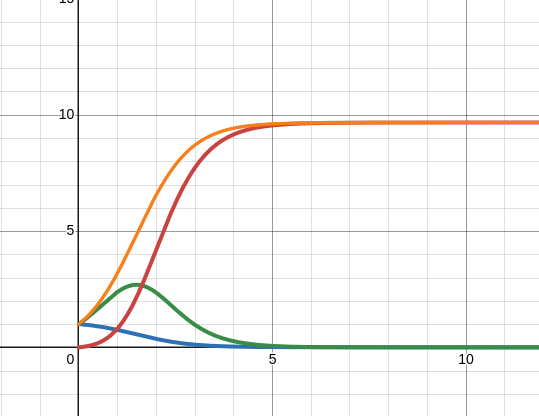
\includegraphics[width=\textwidth]{chapter5/IMG_ch5/QSmean/QS1} % Adjust the image path as necessary
        \caption{When $\mu = 0$.}
        \label{fig:figure1}
    \end{subfigure}
    \hspace{\fill} % Optional: adds space between figures
    % Second figure
    \begin{subfigure}{0.47\textwidth}
        \centering
        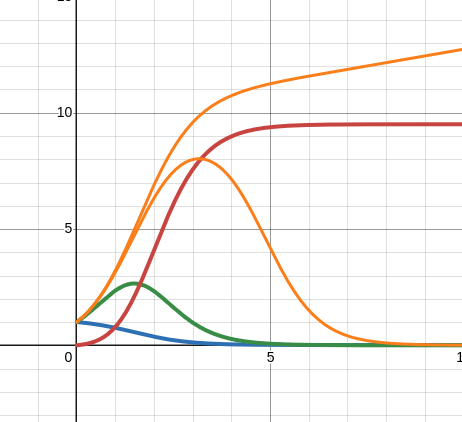
\includegraphics[width=\textwidth]{chapter5/IMG_ch5/QSmean/QS2} % Adjust the image path as necessary
        \caption{When $\mu > 0$.}
        \label{fig:figure2}
    \end{subfigure}
    
    \caption{In the image on the right, the conditional mean (yellow) going up at late time is the mean conditioned on $\xt \neq0$: $J(t)/\hat I(t)$. The yellow line tending to 0 is for the mean conditioned on non-catastrophe $\mean{\xt|\xt \neq R}$}
    \label{fig:two_figures}
\end{figure}



Considering the no-death $\mu = 0$ case on the left above,  it can be easily seen that the conditional mean (yellow) tends to the same limit as $V(t)$, which is shown in red.  That is 

$$\lim_{t\to\infty}     \frac{J(t)}{I(t)}     =    \lim_{t\to\infty} V(t)  = 1 + \frac{\lambda}{\delta}.$$

Here,  when $\delta$ shrinks to 0, the QS mean and expected release count tend to infinity.  








\section{Burst size distribution}

Using 

$$ \int p_k(t)\dd t  = (n\beta)^{-1} \lrb{\frac{{1-\ee^{\beta(a-b)t}}}{{b - a\ee^{\beta(a-b)t}} } }^{n},$$

the following equation can be approached. 


$$\pr{K = k} = \delta k \int_0^\infty p_k(t)\dd t$$
Where $p_k(t) = \pr{\xt = k}$. We have above determined that 

$$p_k(t) =\lrb{ \frac{ a-b }{{b - a\ee^{\beta(a-b)t}}}}^2 \ee^{\beta(a-b)t} \lrb{\frac{{1-\ee^{\beta(a-b)t}}}{{b - a\ee^{\beta(a-b)t}} } }^{k-1}.$$
Then, we have the formula

$$\pr{K = k} = \delta k \int_0^\infty p_k(t)\dd t$$
The current goal is to verify this using Gillespie algorithm simulations. First, we have the integration,

$$\int p_k(t)\dd t  = (k\beta)^{-1} \lrb{\frac{1 - \ee^{\beta(a-b)t}}{b - a\ee^{\beta(a-b)t}}}^k $$
Which can be verified with reverse differentiation (found with Wolfram Alpha). With this,

$$\pr{K=k} = \frac{\delta}{\beta}\lrbs{ \lrb{\frac{1 - \ee^{\beta(a-b)t}}{b - a\ee^{\beta(a-b)t}}}^k}^\infty_0 = \frac{\delta}{\beta}\lrb{\frac{1}{a}}^k$$

$$\pr{K=k} = \frac{\delta}{\beta}\lrb{\frac{1}{\frac{\beta+\mu+\delta}{2\beta} + \sqrt{\lrb{\frac{\beta+\mu+\delta}{2\beta}}^2 - \frac{\mu}{\beta}}}}^k$$






\section{Further considerations}

From 
\begin{align}
\mean{K} &= \mean{K| \tau > t} \pr{\tau > t} + \mean{K| \tau < t}\pr{\tau<t},\\
&= \mean{K|\tau > t} I(t) + \frac{V(t)}{1 - I(t)} \lrb{1 - I(t)},
\end{align}
We find,
$$\mean{K| \tau > t}  = \frac{\mean{K} - V(t)}{I(t)}   =   \frac{  \sum^{\infty}_{k} k \pr{K = k}  - V(t)}{I(t)}$$

Note: $\mean{K} = V_{\text{inf}} = \frac{\lambda - \mu}{\delta} \lrb{1 - I_-} + 1$ (check). Actually, there is some complication. $V(t) = \mean{\yt}$ where $\yt$ is the number of agents ``released''. Basically, at the rupture event, the value of $\xt$ immediately before catastrophe becomes the value of $\yt$. $\yt$ is otherwise 0. What I'm getting at is that $V(t\to \infty)$ does not only represent the average burst size. When $\mu > 0$, some processes will go extinct without catastrophe. In these cases, $\yt$ will remain 0. $V(t) = \mean{\yt}$ captures these processes in its quantity. So if we want to extract the true burst size mean from $V(t)$, we must somehow condition on the processes that did reach rupture. 

$$V(t) = \mean{\yt}$$ 
Whether the catastrophe event has taken place or not can be represented by the truth of $\yt>0$, as the minimum burst size is 1. Rupture has occurred with probability $1 - I(t)$.
$$\mean{\yt} = \mean{\yt|\yt > 0}(1-I(t)) + {\mean{\yt | \yt = 0}}I(t)$$
Since $ {\mean{\yt | \yt = 0}} = 0,$
$$\mean{\yt} = \mean{\yt|\yt > 0}(1-I(t))$$
$$ \mean{\yt|\yt > 0} = \frac{\mean{\yt}}{1-I(t)}.$$
This can be thought of as $\mean{\text{Burst size } | \text{ burst has happened}}$. Note equivalence to a term written above:
$$\mean{K | \tau < t} =\frac{V(t)}{1-I(t)}. $$
So, the overall expected burst size --- the expected size of an arbitrarily generated burst --- is the late time value of this expression: 
$$\mean{K} = \lim_{t\to \infty} \lrb{\mean{K| \tau < t}} = \frac{V_{\text{inf}}}{1 - I_-}.$$
$$\mean{K} = \frac{\frac{\lambda - \mu}{\delta}(1-I_-) + 1}{1-I_-} = \frac{\lambda - \mu}{\delta} + \frac{1}{1-I_-}.$$

Hence, 
$$\mean{K|\tau > t} = \frac{\frac{V_{\text{inf}}}{1 - I_-} - V(t)}{I(t)} =  \frac{\frac{\lambda - \mu}{\delta} + \frac{1}{1-I_-} - V(t)}{I(t)}.$$

Though, there is a curious circularity to this which I'm yet to fully understand. Look what happens when we take $\mean{K|\tau> t}$ at its late time value. 

$$\lim_{t\to\infty}\mean{K|\tau > t} = \frac{\frac{V_{\text{inf}}}{1 - I_-} - V_{\text{inf}}}{I_-}  = \frac{V_{\text{inf}}}{1 - I_-} = \mean{K}$$
Maybe this is an obvious result, but I am yet to fully grasp why.













\section{Potential application in BMVR}




\noindent
Consider a reasonably large population of cells initially infected all by a single \ft $\; $bacteria. Over time, each cell acts independently as a birth death catastrophe process described by the usual quantities, $J$ and $I$. Say there were $N_0$ of such cells at the beginning; as the model progresses there will be approximately $N_0 I(t)$ cells which are yet to rupture. This estimate becoming increasingly accurate with progressively larger $N_0$.\par
In previous work, the quantity, $V(t)$, has been used to describe the count of bacteria released from a single cell. In that application, it has been found to increase at a rate proportional to the second moment of intracellular count, $\delta \mean{\xt^2}$. In this case of $N_0$ initially infected cells, there doesn't seem to be an issue with the same quantification being used --- there being $\Vt(t) = N_0 V(t)$ extracellular bacteria through time (assuming no reabsorption or replication in the extracellular population).\par 

\subsubsection*{Proportional release formula}

But I'm curious about another way $\Vt$ might be quantified. As a starting point, suppose $N_0$ is very large, and that we begin observing the model at a reasonably late start-time, $t_s$. Late enough for convergence to the quasi-stationary distribution in $\xt$. We have previously computed this limiting conditional distribution and its mean: $\mean{\xt | \xt\notin\{R, 0\}}_{t\to\infty}$ and $\pr{\xt = k | \xt\notin\{R, 0\}}_{t\to\infty}$. \par
Through this period of time, it seems the rate of extracellular release, $\dd \Vt/ \dd t$, should be made up of the number of infected cells remaining, $N_0 \hat I(t_s + t)$, ($\hat I $ being the non-fixation probability), multiplied by the expected number in each cell, $\mean{\xx_{t_s + t} | \xx_{t_s + t}\notin\{R, 0\}}_{t\to\infty}$.

$$\ddt{\Vt} = N_0 \hat I(t_s + t) \cdot \mean{\xx_{t_s + t} | \xx_{t_s + t}\notin\{R, 0\}}_{t\to\infty}$$


\noindent
(for $t> t_s$, the stationarity time). In principle, we might be able to compute $\Vt$ in this way.\par
There is an apparent issue with this arrangement, which is: at late time, as the mean bacterial count becomes stationary, it is also true that the non-fixation probability tends towards 0. This could be mitigated by assuming $N_0$ is sufficiently large. Or, say for example we don't know when the infection began, or how many bacteria it started with. But suppose we do know the current concentration of infected cells in the blood, and, we know the infection has been going on long enough for contents of remaining infected cells to be near the stationary distribution. (Of course, this now assumes reabsorption). In this case, the infected cell count, $N_0 \hat I(t_s + t)$, would be taken as a constant --- call it $\Ic$. And, the factor multiplying it in the release rate would merely be the QS mean (which we have a formula for):

$$\ddt{\Vt} = \Ic\cdot \mean{\xx_{t} | \xx_{t}\notin\{R, 0\}}_{t\to\infty}$$

Important to recognise this now assumes reabsorption, but say we roll with the idea.


\subsubsection*{Intuitive argument}

By some intuitive logic of this kind,  it may be feasible to propose a small update to the ``basic model of viral replication'':\par
From this,

\begin{align*}
\ddt{I} &= \beta T V - \delta I\\
\ddt{V} &= p I - c V
\end{align*}


\noindent
to this,

\begin{align*}
\ddt{I} &= \beta T V - \delta I\\
\ddt{V} &= \lrbs{\mean{\xx_{t} | \xx_{t}\notin\{R, 0\}}_{t\to\infty}} I - c V
\end{align*}


\noindent
Where the only difference is that the constant viral release rate, $p$, has been replaced by a slightly more complicated constant value which is a combination of intra-cellular rates.

$$p = \mean{\xx_{t} | \xx_{t}\notin\{R, 0\}}_{t\to\infty} =\quad ?$$ 


\noindent
The purpose of this is that, given someone is in a situation where they have a good estimate for $p$, the viral release rate, by our logic, they may then be able to access an approximation for the rates constituting the QS mean. \par

\vspace{15pt}


\noindent
(need to look up the formula for QS mean, but its something like $\lim_{t\to\infty}{J(t) / (1-\hat I(t))}$. I think there is an important point around whether $\mu = 0$ or not.)


\subsubsection*{Towards a correction}

The above formula is incorrect, but there might be a way to fix it. The problem is that the burst rate depends on intracellular load.


We can use the approximation which assumes that the distribution of cell infection sizes is at its late-time stationary value. Or maybe this isn't the best option. Because at any time, there will be infected cells that begin their infection dynamics at a number of different start times. The distribution of release times is given by a known formula. So Perhaps there is some way of combining this time pdf and the second-moment formula conditional on time in a normalization. 

Is it an integral:

$$p =  \delta \int \phi(t) \mean{\xt^2 | \xt \notin \{R, 0 \} }(t)  \dd t$$

(The second moment conditional on non-rupture, normalized over the probability density of burst times ) Where $\phi(t)$ is the known pdf of rupture times. \par
Or is it this:


$$p = \int \phi(t) \mean{R | \tau = t} \dd t$$

(The rupture size probability given burst time, normalized over the probability density of burst times)


\subsubsection*{Iterating cycles --- overall expected release rate?}
The quantity this is trying to represent can be thought of simply as follows. Consider a model where at first there is a single infected macrophage. When it ruptures, each of the output bacteria go on to found a new BDC process in a new infected cell. Until, at different times, each of these ends in turn and cycles continue with new intracellular infectious processes beginning and ending, beginning and ending.\par

Over a sufficient period of time following the initial cell, there will emerge a sort of stationarity whereby any given release event will exhibit a burst time and burst size according to the known distributions. Short-duration processes will by nature occur more frequently than longer-duration ones. 


{ What we desire is an overall rate of release events and their sizes to make up an approximation to replace the} $p I $ {term in the Basic Model of Viral Replication above.}


{For any given cell, the probability that it will burst soon will be higher if it has a high internal census. But large bursts, in this population cyclic dynamic will be less frequent because short release times with smaller bursts happen with a greater frequency. }














































\chapter{Birth death catastrophe -- Two type and $N=2$}





















































%%%%%%%%%%%%%%%%%%%%%%%%%%%%%%%%%%%%%%%%%%%%%%%%%%%%%%%%%%%%%%%%%%%%%%%%%%%%%%%%%%%%%%%%%%%%%%%%%%%%%%%%%%%%%%%%%%%%%%

\section{Two type}







For now, let us consider the non-catastrophe probabilities, 
$$ S(t) = \pr{\neg\lrb{\xt = \yt = R}| \xx_0 = 1} $$ 
$$G(t) = \pr{\neg\lrb{\xt = \yt = R}| \yy_0 = 1}.$$
Recalling that each population undergoes birth and death; units of $\xt$ can mutate (one way), adding to $\yt$; and any unit from either population can trigger catastrophe --- a transition to $(\xt, \yt) = (R, R)$:
\begin{align*}
\pr{\Delta \xt = 1} &=  {\lambda_1} \xt \delt, && \text{(birth)}\\
\pr{\Delta \xt = -1} &=  \hat\mu_1 \xt \delt, && \text{(death)}\\
\pr{\Delta \xt = -1,  \Delta \yt = 1} &=  \hat\nu \xt \delt, && \text{(mutation)}\\
\pr{ \Delta \yt = 1} &=  \hat\lambda_2 \yt \delt, && \text{(birth)}\\
\pr{ \Delta \yt = -1} &=  \hat\mu_2 \yt \delt, && \text{(death)}\\
\pr{ \xdt = R,   \ydt = R} &=  \hat\delta ( \xt  + \yt) \delt. && \text{(catastrophe)}
\end{align*}
Later, it should be seen that the same methods will apply to the almost identical Riccati equations encoding for probability generating functions. The only real difference will be in initial conditions. \par

The equations are as follows.
\begin{align}
\frac{\dd S}{\dd \hat t} &= \lambda_1 S^2 - (\lambda_1 + \hat\mu_1 + \hat\nu + \hat\delta) S + \hat\mu_1 + \hat\nu G,\label{S1a}\\
\frac{\dd G}{\dd \hat t} &= \hat\lambda_2 G^2 - (\hat\lambda_2 + \hat\mu_2 + \hat\delta) S + \hat \mu_2, \label{G1a}
\end{align}
Initial conditions: $S(0) = G(0) = 1$. Scaling time, we can remove $\lambda_1$ from the first equation. With $\hat t =  \lambda_1^{-1} t$, 
$$\frac{\dd S}{\dd \hat t} \rightarrow \lambda_1 \ddt S.$$
And with each other parameter redefined in scaled form, $\mu_1 \equiv \frac{\hat\mu_1}{\lambda_1}$, ($\nu \equiv \frac{\hat \nu}{\lambda_1}$, etc ...) equations (\ref{S1a}) and (\ref{G1a}) become,
\begin{align}
\frac{\dd S}{\dd  t} &= S^2 - (1 + \mu_1 + \nu + \delta) S + \mu_1 + \nu G \label{S1b}\\
\frac{\dd G}{\dd  t} &= \lambda_2 G^2 - (\lambda_2 + \mu_2 + \delta) S +  \mu_2 \label{G1bhh}
\end{align}
It is these we will try to solve. 




\subsection{General case}

As key steps, the process will run as follows. \\


\begin{adjustwidth}{1cm}{}
\begin{itemize}
\item[\textbf{Step 1.}] Rescale (\ref{G1bhh}) with $G(t) = a K(t) + b$ into the form, 
\begin{align}
\ddt K &= \lambda_2 \lrb{ P K^2 - (P+Q)K + Q}, \nonumber\\
&= \lambda_2(PK-Q)(K-1) \label{thisForm}
\end{align}
with $P\equiv P(a,b)$, $Q\equiv Q(a,b)$ to be determined. \\

\item[\textbf{Step 2.}] Permitted by step 1, write $K(t)$ in the form $K(t) = 1 - F(z(t))$, where
\begin{itemize}
\item $F(Z) \propto (1-z(t))^{-1}$, and 
\item $z(t)\propto \ee^{qt}$, for some $q < 0$.\\
\end{itemize}

\item[\textbf{Step 3.}] Substitute the resulting $G(t) = aK(t) + b = a[1 - F(z(t)] + b$ into (\ref{S1b}):
$$\frac{\dd S}{\dd  t} = S^2 - (1 + \mu_1 + \nu + \delta) S + \mu_1 + \nu \{ a[1 - F(z(t)] + b\}.$$
And rescale $S(t)\equiv X + h$, with $h$ chosen to eliminate constant terms. \\

\item[\textbf{Step 4.}] Apply the standard Riccati trick to convert into a Sturm–Liouville equation. \\

\item[\textbf{Step 5.}] Use asymptotic linearisation to inform an anzat trial function.\\

 \item[\textbf{Step 6.}] With substitution, retrieve the hyper-geometric canonical form. And loop back through the steps to define a final solution. \\
\end{itemize}
\end{adjustwidth}

\noindent
Steps 3, 4, 5, and 6 being analogous to those made by Antal and Krapivsky. Their similar equations were already in a form like (\ref{thisForm})

\subsubsection{Step 1. Rescale $G(t)$}


\begin{lemma}
\label{lemma1}
    Using the substitution $G(t) = aK(t) + b$, where 
    $$a = 1 + 2\sqrt{\lrb{\frac{\lambda_2+\mu_2+\delta}{2\lambda_2}}^2 - \frac{\mu_2}{\lambda_2}},$$
    $$b = \frac{\lambda_2+\mu_2+\delta}{2\lambda_2} -1 - \sqrt{\lrb{\frac{\lambda_2+\mu_2+\delta}{2\lambda_2}}^2 - \frac{\mu_2}{\lambda_2}}, $$
    we can transform
    $$\frac{\dd G}{\dd  t} = \lambda_2 G^2 - (\lambda_2 + \mu_2 + \delta) S +  \mu_2 \label{G1b}$$
    into
    $$\ddt{K} = \lambda_2\lrbs{PK^2 -(P+Q)K + Q}$$
    with 
    $$P=a \quad\text{and}\quad Q=1.$$
    Which can be written as
    \begin{align*}
	\ddt{K} &= \lambda_2(PK-Q)(K-1),\\
	&= \lambda_2(aK-1)(K-1).
   \end{align*}
\end{lemma}

\noindent
We will define the following constant combinations to simplify the syntax: 
\begin{itemize}
\item $\eta = \frac{\lambda_2+\mu_2+\delta}{\lambda_2}$,
\item $\xi = \frac{\mu_2}{\lambda_2}$,
\item $C^* = \lrb{\frac{\eta}{2}}^2 - \xi $,\\
\end{itemize}
hence
\begin{itemize}
\item $a = 1 + \sqrt{C^*}$,
\item $b = \frac{\eta}{2} - 1 - \sqrt{C^*}$.
\end{itemize}

\vspace{15pt}

\noindent
\textbf{proof.} To begin, we substitute $G(t) = a K(t) + b$ into (\ref{G1bhh}):
    $$a \ddt K = \lambda_b\lrbs{(aK+b)^2 - \eta(aK+b) + \xi},$$
    writing $ \eta = (\lambda_b + \mu+b + \delta) / \lambda_b$ and $\xi = \mu_b / \lambda_ b$. This rearranges to 
    $$ \ddt K = \lambda_b\lrbs{ a K^2 - \lrb{\eta - 2b} K + \frac{1}{a} \lrb{b^2 -\eta b + \xi}}.$$
    Forcing 
    \begin{equation}
    \label{conditionFirst}
\ddt{K} = \lambda_2 \lrbs{ P k^2 - (P+Q)K + Q}
\end{equation}
    for some  $P\equiv P(a,b)$ and $Q\equiv Q(a,b)$, gives three conditions: 
   
  \begin{subequations}\label{eqn:binomi}
    \begin{align}
      P  &= a \label{cond1} \\
      P + Q &= \eta - 2b \label{cond2} \\
      Q&= \frac{1}{a} \lrb{b^2 - \eta b + \xi} \label{cond3}
    \end{align}
  \end{subequations}
  Taking first (\ref{cond3}),
  $$b^2 - \eta b + \xi - aQ = 0$$
  $$\lrb{b-\frac{\eta}{2}}^2 - \lrb{\frac{\eta}{2}}^2 + \xi - aQ = 0$$
  so
  \begin{equation}
  \label{bplusminus}
   b_{\pm} = \frac{\eta}{2} \pm \sqrt{\lrb{\frac{\eta}{2}}^2 -\xi + aQ}.
  \end{equation}
  
  \noindent
 Then looking to (\ref{cond2}), with substitution of $b_\pm$,
 
 $$\eta - 2 \lrbs{\frac{\eta}{2} \pm \sqrt{\lrb{\frac{\eta}{2}}^2 - \xi + aQ} } = P +Q = a + Q \quad\text{ (with (\ref{cond1}))}.$$
For simplicity, define $C^* \equiv\lrb{\frac{\eta}{2}}^2 - \xi  $,
$$ \cancel{\eta - \eta }  \pm 2 \sqrt{C^* +aQ} = {a+Q}$$
Hence
$$4\lrb{C^* +aQ} =  \lrb{a+Q}^2.$$

\noindent
Note: going back a step here is sign sensitive. This turns out to be important in our selection of $b_-$ over $b_+$.\\ Then,
$$a^2 - 2Qa + Q^2 - 4C^* = 0$$
$$(a-q)^2 -\cancel{Q^2 +Q^2} - 4C^* = 0$$
so
$$a_\pm = Q \pm 2\sqrt{C*}$$
Since the system of equations (\ref{cond1}) - (\ref{cond3}) is overdetermined, we can choose $Q$ arbitrarily. Setting it to one,
\begin{equation}
\label{aplusminus}
a_\pm = 1 \pm 2\sqrt{C*}
\end{equation}
And taking the positive choice, $a_+$, we can simplify $b$. Substituting (\ref{aplusminus}) into (\ref{bplusminus}), 

$$b_{\pm} = \frac{\eta}{2} \pm \sqrt{  C^* +  \lrbs{ 1 \pm 2\sqrt{C*}  }}.$$ 

\noindent
The choice of $+$ or $-$ in $a$ seems arbitrary; but in verification, it proves important to select the negative sign in $b$. The check is made by starting again from the beginning with substitution of $G(t) = aK(t) + b$ with $a$ and $b$ as defined. It can be shown that provided the $b_-$ is chosen, the transformation yields

$$\ddt K = \lambda_2\lrbs{aK^2 - (a + 1)K + Q}.$$

\noindent
like (\ref{conditionFirst}). Which, as required, can be written

$$\ddt K = \lambda_2{(aK-1)(K-1)}.$$

\qed



\subsubsection{Step 2. Rearrange $K(t)$}

\begin{lemma}
The function $K(t)$, in accordance with 
\begin{equation}
\label{eqdesk}
 \ddt K = \lambda_2 (aK - 1)(K-1)
\end{equation}
(initial condition $G(0) = 1 = aK(0) + b$), can be written as
$$K(t) = 1-F(z(t)),$$
where 
$$z(t) = \lrb{\frac{b}{a+b-1}} \ee^{\lambda_2 (1-a) t},$$
and 
$$F(z) = \frac{a^{-1}(a-1)}{1-z}.$$
\end{lemma}


\noindent
\textbf{proof.} Starting with the equation describing $K(t)$, (\ref{eqdesk}), a separable ODE. It can be solved by integrating:
$$\int\frac{1}{(aK - 1)(K-1)}\dd K = \lambda_2\int\dd t.$$
With partial fractions,
$$(1-a)^{-1}\int\lrb{\frac{a}{aK-1} - \frac{1}{K-1}}\dd t = \lambda_2\int\dd t.$$
 
$${\ln(aK-1) - \ln(K-1)} = \lambda_2 (1-a) t + \text{const.}$$
becoming
$$\ln\lrb{\frac{aK-1}{K-1}} = \lambda_2 (1-a) t + \text{const.} $$
Fixing the constant with initial condition, $K(0) = a^{-1}(1-b)$ (from $G = aK +b$),

$$\ln\lrb{\frac{ab}{a+b - 1}}  = 0 + \text{const.}$$
Hence
$${\frac{aK-1}{K-1}} =  \lrb{\frac{ab}{a+b - 1}}   \ee^{ \lambda_2 (1-a) t } = \mathcal{W} \quad\text{(temporary, for derivation)},$$
and, rearranging for $K(t)$,
\begin{align*}
aK -1 &= \mathcal{W} (K-1), \\
(a - \mathcal{W})K &= 1 - \mathcal{W}\\
K &= \frac{1-\mathcal{W}}{a - \mathcal{W}}\\
K &= \frac{1 - \lrb{\frac{ab}{a+b-1}} \ee^{\lambda_2 (1-a) t} }{a - \lrb{\frac{ab}{a+b-1}} \ee^{\lambda_2 (1-a) t} }\\
K &= \frac{(a+b-1) - \lrb{{ab}} \ee^{\lambda_2 (1-a) t} }{a(a+b-1) - \lrb{{ab}} \ee^{\lambda_2 (1-a) t} }
\end{align*}
Extracting a one with the following trick,
\begin{align*}
K &= \frac{(a+b-1) - \lrb{{ab}} \ee^{\lambda_2 (1-a) t}   + \lrbs{  a(a+b-1) - \lrb{{ab}} \ee^{\lambda_2 (1-a) t}} - \lrbs{a(a+b-1) - \lrb{{ab}} \ee^{\lambda_2 (1-a) t}  } }{a(a+b-1) - \lrb{{ab}} \ee^{\lambda_2 (1-a) t} }\\
K &= \frac{a(a+b-1) - \lrb{{ab}} \ee^{\lambda_2 (1-a) t} }{a(a+b-1) - \lrb{{ab}} \ee^{\lambda_2 (1-a) t} }  +  \frac{(a+b-1) - \cancel{\lrb{{ab}} \ee^{\lambda_2 (1-a) t}}  - {a(a+b-1) + \cancel{\lrb{{ab}} \ee^{\lambda_2 (1-a) t} } } }{a(a+b-1) - \lrb{{ab}} \ee^{\lambda_2 (1-a) t} }\\
K &=  1 - \frac{(a-1)(a+b-1)}{a(a+b-1) - \lrb{{ab}} \ee^{\lambda_2 (1-a) t}}\\
K &=  1 - \frac{a^{-1}(a-1)}{1 -  \lrb{\frac{b}{a+b-1}} \ee^{\lambda_2 (1-a) t}}
\end{align*}
Which, if you squint at it, is in the desired form. That is, $K(t) = 1 - F(z(t))$;
$$K = 1 - \frac{a^{-1}(a-1)}{1-z(t)},$$
with 
\begin{equation}
\label{ansatseed}
z(t) = \lrb{\frac{b}{a+b-1}} \ee^{\lambda_2 (1-a) t}
\end{equation}

\qed

\noindent
At late time, $t\to\infty$, $z(t)\to 0$, and hence, $F(t)\to a^{-1}(a-1)$.
    



\subsubsection{Step 3. Substitute rescaling of $G(t)$}



\begin{lemma}
With substitution of $S(t) \equiv X(t) + h$, where
\begin{align*}
h &= \frac{\lambda_1 + \mu_1 + \nu + \delta}{2} + \sqrt{\lrb{\frac{\lambda_1 + \mu_1 + \nu + \delta}{2}}^2 - \mu_1 - \nu(a+b)}\\
h &= \frac{\kappa}{2} + \sqrt{\lrb{\frac{\kappa}{2}}^2 - \mu_1 - \nu(a+b)}
\end{align*}
($\kappa = \lambda_1 + \mu_1 + \nu + \delta$), a transformation can be made, using 
\begin{align*}
G(t) &= aK(t) + b\\
 &= a(1-F(z(t))) + b,
\end{align*}
of 
\begin{equation}
\label{SwithF}
\ddt S = S ^2 - (\lambda_1 + \mu_1 + \nu + \delta)S + \mu_1 + \nu (a(1-F) + b)
\end{equation}
into 
$$\ddt X = X^2 + (2h-\kappa)X - \nu a F$$

\end{lemma}


\noindent
\textbf{proof.} Starting with (\ref{SwithF}), substitute $S\equiv X+h$, with $h$ to be determined:
\begin{align*}
\ddt X &= (X+h)^2 - \kappa(X+h) + \mu_1 + \nu(a+b) - \nu a F\\
&= X^2 + (2h-\kappa)X - \nu a F+ \lrbs{h^2  - \kappa h + \mu_1 + \nu (a+b)} 
\end{align*}
Now, select $h$ such that what's inside the square bracket becomes 0.
$$h^2  - \kappa h + \mu_1 + \nu (a+b)=0$$
$$\lrb{h-\frac{\kappa}{2}}^2 - \lrb{\frac{\kappa}{2}}^2 + \mu_1 + \nu(a+b) = 0$$
$$h = \frac{\kappa}{2} \pm \sqrt{\lrb{\frac{\kappa}{2}}^2  - \mu_1 - \nu(a+b)}.$$
We can select the positive sign arbitrarily. 
\qed




\subsubsection{Step 4. Strum-Liouville from Riccati trick}
 Leading on from the previous step, we have an equation describing $S(t)$ in terms of $X(t)$:
 \begin{equation}
 \label{theXeq}
\ddt X = X^2 + (2h-\kappa)X - \nu a F
\end{equation}
In the 4th step we will convert this Riccati equation to a Strum-Liouville: 
$$\frac{\dd^2 Z}{\dd t^2} + (\kappa - 2h ) \ddt Z - \nu a F Z = 0. $$
This is achieved with a standard trick for Riccati equations, 
$$X = -\frac{1}{Z}\ddt Z.$$
From (\ref{theXeq}) it follows that,
$$\cancel{\frac{1}{Z^2}\lrb{\ddt Z}^2 } - \frac{1}{Z}\frac{\dd^2 Z}{\dd t}  =  \cancel{\frac{1}{Z^2}\lrb{\ddt Z}^2 } - (2h - \kappa) \frac{1}{Z^2}\lrb{\ddt Z}  - \nu a F ,$$
which as expected becomes, 
\begin{equation}
\label{StLio}
\frac{\dd^2 Z}{\dd t^2} + (\kappa - 2h ) \ddt Z - \nu a F(z(t)) Z = 0. 
\end{equation}


\subsubsection{Step 5. Asymptotic linearisation}

In the late time limit, $t\to\infty$, $F(z(t))$ tends to a constant, $F\to F_{\infty} =  a^{-1}(a-1)$. Meaning that the above equation will tend to the form of a linear second order ODE, 

$$\frac{\dd^2 Z}{\dd t^2} + (\kappa - 2h ) \ddt Z - \nu a F_\infty Z = 0,$$
with a solution defined proportionally,
$$Z_{t\to\infty} \propto \ee^{\omega t},$$
omega satisfying,
\begin{equation}
\label{passTheAux}
\omega^2 + (\kappa - 2h) \omega - \nu a F_\infty = 0
\end{equation}
From (\ref{ansatseed}), $\ee^t$ can be defined in terms of $z$,
$$\ee^t = \lrb{\frac{a+b-1}{b}}z^{\frac{1}{\lambda_2 (1-a)}}.$$
and so the late time behaviour of (capital) $Z$, can be understood as a function proportional to $z$,
$$Z_{t\to\infty}\propto z^{\frac{\omega}{\lambda_2(1-a)}}.$$
Assuming some correction factor from $Z_{t\to\infty}(t)$ to $Z(t)$: $\Phi(z(t))$. That is 
$$Z = z^{\frac{\omega}{\lambda_2(1-a)}} \Phi(z).$$
$\Phi$ tending to a constant at late time, 
We can use this formula as an ansat, a trial function, to seek the form of the correction, $\Phi$, in terms of $z$. We begin by substituting the ansat, $z^k\Phi(z)$ into (\ref{StLio}), but first, for simplicity, let's define 
$$q = \lambda_2(1-a) \quad\text{and}\quad k = \frac{\omega}{q},$$
notice
$$Z = z^{k} \Phi(z) \quad\text{and}\quad  z = \lrb{\frac{b}{a+b-1}} \ee^{qt},$$
and 
$$\ddt z = q z.$$
To make the substitution, it will be necessary to compute $\frac{\dd Z}{\dd t}$, and $\frac{\dd^2 Z}{\dd t^2}$:
\begin{itemize}
\item $\ddt Z = q z^k \lrbs{z\Phi' + k\Phi}$
\item $\displaystyle\frac{\dd ^2 Z}{\dd t^2} = q^2 z^k \lrbs{z^2 \Phi'' + (2k+1)z\Phi' + k^2\Phi}$
\end{itemize}

\subsubsection{Step 6. Constructing the Hypergeometric canonical form}

With the above computations of $\frac{\dd Z}{\dd t}$, and $\frac{\dd^2 Z}{\dd t^2}$, we can make the substitution of $Z = z^k\Phi(z)$ into (\ref{StLio}): 
$$\frac{\dd^2 Z}{\dd t^2} + (\kappa - 2h ) \ddt Z -   \nu a \frac{a^{-1}(a-1)}{1-z} Z = 0, $$
becomes
$$q^2 z^k \lrbs{z^2 \Phi'' + (2k+1)z\Phi' + k^2\Phi}+ (\kappa - 2h ) q z^k \lrbs{z\Phi' + k\Phi}-  \nu  \frac{(a-1)}{1-z} z^k\Phi(z) = 0.$$
Since $z\neq 0$ for finite time, we can divide a factor of $z^k$. Then, after collecting orders, $\Phi$, $\Phi'$, and $\Phi''$, we find,
\begin{equation}
    \label{curlyBs}
    q^2 z^2 \Phi''  + \lrbs{q^2(2k+1) + q(\kappa - 2h)}  z\Phi'  + \lrbc{q^2 k^2 + qk(\kappa - 2h) - \nu  \frac{(a-1)}{1-z}} \Phi = 0.
    %q^2 z^2 \Phi'' + \lrbs{q^2(2k+1) + q(\kappa - 2h)}z\Phi' + \lrbc{q^2 k^2 + qk(\kappa - 2h) - \nu  \frac{(a-1)}{1-z}} \Phi = 0.
\end{equation}
Here's the trick; the reason why this choice of ansat is useful. But first, we must see the equation in terms of the constants obscured by the definition of $q = \lambda_2 (1-a)$ and $k = \omega / q$. For the present purpose, we can consider only terms within the curly brackets of  (\ref{curlyBs}): 
\begin{align*}
 &\lrbc{q^2 k^2 + qk(\kappa - 2h) - \nu   \frac{(a-1)}{1-z}}\\
 = &\lrbc{q^2 \lrb{\frac{\omega}{q}}^2 + q\lrb{\frac{\omega}{q}}(\kappa - 2h) - \nu  \frac{(a-1)}{1-z}}\\
   =&\lrbc{\omega^2 + \omega(\kappa - 2h) - \nu  \frac{(a-1)}{1-z}}.
\end{align*}
Notice the form of our auxiliary equation above, ($\ref{passTheAux}$):
$$\omega^2 + (\kappa - 2h) \omega - \nu a F_\infty = 0.$$
From it, 
$$\omega^2 + (\kappa - 2h) \omega  =  \nu a F_\infty = \nu (a - 1).$$
Thus, going back to the curly brackets, 
\begin{align*}
   &\lrbc{\nu (a - 1)- \nu  \frac{(a-1)}{1-z}}\\
   =&\lrbc{\nu (a - 1)\lrbs { 1 - \frac{1}{1-z}}}\\
   =&\lrbc{\nu (a - 1)\lrbs { - \frac{z}{1-z}}}.
\end{align*}
And with substitution of this back into (\ref{curlyBs}), we get
$$q^2 z^2 \Phi'' + \lrbs{q^2(2k+1) + q(\kappa - 2h)}z\Phi' + \nu(a-1)\lrb{ \frac{z}{1-z}}\Phi = 0.
$$
Rearranging,
$$ (1-z)z \Phi'' + \lrbs{(2k+1) + \frac{\kappa - 2h}{q}  }(1-z)\Phi' + \frac{\nu(a-1)}{q^2}\Phi = 0.
$$
And with $q = \lambda_2 (1-a)$,
$$ (1-z)z \Phi'' + \lrbs{(2k+1) + \frac{\kappa - 2h}{\lambda_2 (1-a)}  }(1-z)\Phi' - \frac{\nu}{\lambda_2^2(1-a)}\Phi = 0.
$$
Finally,
$$ (1-z)z \Phi'' + \lrbs{ \frac{\kappa - 2h}{\lambda_2 (1-a)} + 2k+1  - \lrb{    \frac{\kappa - 2h}{\lambda_2 (1-a)} + 2k+1    }z }\Phi' - \frac{\nu}{\lambda_2^2(1-a)}\Phi = 0.
$$
Which is in the canonical hypergeometric form, 
$$ (1-z)z \Phi'' + \lrbs{ C  - \lrb{  A + B + 1  }z }\Phi' -AB\Phi = 0.
$$



\subsubsection{Step 7. The Canonical form constants}


Substituting $k = \omega / q$, the final hypergeometric form from the previous section becomes
$$ (1-z)z \Phi'' + \lrbs{ \frac{2\omega + \kappa - 2h}{\lambda_2 (1-a)} +1  - \lrb{    \frac{2\omega + \kappa - 2h}{\lambda_2 (1-a)} + 1    }z }\Phi' - \frac{\nu}{\lambda_2^2(1-a)}\Phi = 0.
$$
Comparing this to
$$ (1-z)z \Phi'' + \lrbs{ C  - \lrb{  A + B + 1  }z }\Phi' -AB\Phi = 0,
$$
we find the constants $A$, $B$, $C$. Firstly from the final term,
$$A = B^{-1} \frac{\nu}{\lambda_2^2(1-a)};$$ 
Then from $A+B+1 = C$ at the second term,
$$B = -\frac{1-C}{2} \pm \sqrt{\lrb{\frac{1-C}{2}}^2 -  \frac{\nu}{\lambda_2^2(1-a)}}.$$
So with $C$ as given directly in the second term:
\begin{align*}
C &=   1 - \frac{2\omega + \kappa - 2h}{\lambda_2^2 (1-a)} \\
B  &=  -\frac{2\omega + \kappa - 2h}{2\lambda_2(1-a)}  \pm \sqrt{\lrb{\frac{2\omega + \kappa - 2h}{2\lambda_2(1-a)}}^2 - \frac{\nu}{\lambda_2^2 (1-a)}}  \\
A   &=      -\lrb{\frac{2\omega + \kappa - 2h}{2\lambda_2(1-a)}  \pm \sqrt{\lrb{\frac{2\omega + \kappa - 2h}{2\lambda_2(1-a)}}^2 - \frac{\nu}{\lambda_2^2 (1-a)}}}^{-1}\frac{\nu}{\lambda_2^2 (1-a)}
\end{align*}



As a reminder,

\begin{itemize}
\item $h = \frac{\kappa}{2} + \sqrt{\lrb{\frac{\kappa}{2}}^2 - \mu_1 - \nu(a+b)}$
\item $\kappa  = \lambda_1 + \mu_1 + \nu + \delta$
\item $a = 1 + 2\sqrt{\lrb{\frac{\lambda_2+\mu_2+\delta}{2\lambda_2}}^2 - \frac{\mu_2}{\lambda_2}}$
\item $b = \frac{\lambda_2+\mu_2+\delta}{2\lambda_2} -1 - \sqrt{\lrb{\frac{\lambda_2+\mu_2+\delta}{2\lambda_2}}^2 - \frac{\mu_2}{\lambda_2}} $
\item $\omega$ satisfies $\omega^2 + (\kappa - 2h) \omega - \nu a F_\infty = 0$ where $F_\infty = a^{-1}(a-1).$
\end{itemize}





\subsubsection{Step 8. Retrieving the solution}


Going back through the substitutions,

$$S(t) = h + X(t),$$
$$X(t) = -\frac{1}{Z}\ddt{Z},$$
$$Z(t) = z^k\phi(z),$$
It can be shown that 
$$\frac{1}{Z}\ddt{Z} = \omega + \frac{q z}{\phi} \frac{\dd \phi}{\dd z},$$
so
$$S(t) = h - \frac{1}{Z}\ddt{Z}  = h - \omega - \frac{q z}{\phi} \frac{\dd \phi}{\dd z}.$$
From the hypergometric canonical form, there are two linearly independent solutions for $\phi(z)$:

$$F(A,B;C;z) \quad\text{and}\quad z^{1-C}F(A-C+1,B-C+1;2-C;z)$$
So including a parameter ($D$) to be fixed by initial conditions:
$$\phi(z) = F(A,B;C;z)+ D z^{1-C}F(A-C+1,B-C+1;2-C;z).$$
Then, with the differential of the hypergeometric given by an identity,
$$\frac{\dd F}{\dd z} = \frac{AB}{C}F(1+A,1+B;1+C;z),$$
it is merely a small headache to compute the final solution using 
$$S(t)   = h - \omega - \lambda_2(1-a)\frac{ z}{\phi} \frac{\dd \phi}{\dd z}.$$






































%%%%%%%%%%%%%%%%%%%%%%%%%%%%%%%%%%%%%%%%%%%%%%%%%%%%%%%%%%%%%%%%%%%%%%%%%%%%%%%%%%%%%%%%%%%%%%%%%%%%%%%%%


\section{$N = 2$ case}







The following will be a summary of our analytical progress in understanding the chained bursting model. 

We are exploring this area in pursuit of a more general aim to compare and contrast budding and bursting assumptions in models of bacterial and viral pathogenesis. Budding dynamics are widely used in the modelling of viral dynamics. They generally assume that cells and free virions are well mixed, that host cells can be simply infected or not, and that infected cells release new free virions at a steady rate.\par
The bursting assumption models we have been looking at are quite different. Infected cells contain a changeable number of pathogenic particles. In our case, these intracellular dynamics follow a standard birth-death process, or just a birth process, excluding death for tractability. Pathogen isn't released steadily as in budding; the entire content of a host cell is released at its time of rupture, and this event may be brought on by the resident infection itself. \par
So far, we have been successful in describing the mean behaviour of a single host cell through the course of its infection. Our next steps will be in trying to quantify the dynamics of an infection that spreads through a population of host cells. Perhaps in a well-mixed setting, or even with some spatial component. For now, we have simplified the line of questioning to free up tractability. We have considered a chained infection assumption whereby at the rupture of an infected cell, its entire contents are immediately transferred into another host cell from the population. This repeats until one by one, all of the host cells have been infected and have ruptured. 



\subsubsection*{Specifying the model}


To begin with, there are $M$ macrophages, all but one empty with the exception containing a single pathogenic particle. 

This might be quite a reasonable initial condition given that the number of colony-forming units in some diseases is small ($\mathcal{O}(100)$) compared to the number of immune cells in the body.


Macrophage resident pathogenic particles are subject to a standard birth-death process (for now, we consider only the no-death case), and there is also the possibility of a rupture event. This catastrophe will occur at a rate proportional to the number of intracellular particles. On rupture, a macrophage will release all of its pathogenic load, usually into the surrounding extracellular medium, but for our purposes, we assume that it is all immediately transferred into another macrophage, where again a birth-death and rupture process will take place. 

In this way, supposing there is no pathogenic extinction (a certainty in the no-death case), the process will see a total of M macrophage rupture events, of increasing pathogenic load and partitioned by reducing intervals of time. 

Considering the ith of these M catastrophe events, what sort of questions can we ask? So far, we have had some success in describing the rupture counts; the number of pathogenic particles present at the time of a given rupture. For the $i$th of such events, we label this count, $r_i$. And indeed, we have been able to describe the distribution of this quantity for each $i$. There is some technicality to the general case, $i = M$, but this will be covered below. 

The other obvious method of description is in the times at which these catastrophes occur. We assign the label, ti, to the time at which the $i$th rupture takes place. These, along with the interval times, $T_i = t_i - t_{i-1}$, make up the current focus for our analysis. 







\subsubsection*{Results on rupture size distributions}




It was possible to write a general formula for the coefficients!

$$\mathcal{P}(r_k) = \mathrm{Prob}\{r_k = n|X_0=1\}$$

$$\mathcal{P}(r_1) = \left(\frac{\delta}{\delta + \lambda}\right)^{} \left(\frac{\lambda}{\delta + \lambda}\right)^{n-1}$$

$$\mathcal{P}(r_2) = n\left(\frac{\delta}{\delta + \lambda}\right)^{2} \left(\frac{\lambda}{\delta + \lambda}\right)^{n-1}$$

$$\mathcal{P}(r_3) = \frac{n(n+1)}{2}\left(\frac{\delta}{\delta + \lambda}\right)^{3} \left(\frac{\lambda}{\delta + \lambda}\right)^{n-1}$$

$$\mathcal{P}(r_4) = \frac{n(n+1)(n+2)}{6}\left(\frac{\delta}{\delta + \lambda}\right)^{4} \left(\frac{\lambda}{\delta + \lambda}\right)^{n-1}$$


$$\mathcal{P}(r_k) = \mathcal{A}^{(n)}_{k}\left(\frac{\delta}{\delta + \lambda}\right)^{k} \left(\frac{\lambda}{\delta + \lambda}\right)^{n-1}$$


$$\mathcal{A}^{(n)}_{k} = \sum^{n}_{i=1}\mathcal{A}^{(i)}_{k-1}, \hspace{10pt} \mathcal{A}^{(i)}_{1} = 1 \;\; \forall i $$
 and  $\mathcal{A}^{(i)}_2 = i$ because $\sum_{i=1}^n \mathcal{A}_1^{(i)}= \sum_{i=1}^n 1 = n$
$$\mathcal{A}^{(n)}_{k} =  \frac{1}{k!}\frac{(n+k-1)!}{(n-1)!}$$
You can see the pattern of this result emerging in $n=1,2,3$ and 4. Perhaps it is possible to prove it by induction.


\vspace{20pt}

\subsubsection*{Towards rupture time distributions}

In the chained model, the first cell will rupture at some time, $t_1$, distributed according to the probability density function (pdf), $\mathcal{F}_{1}(t) = -\frac{\mathrm{d}S}{\mathrm{d}t}$. This being for the case in which there is only a single initial bacterium. More generally, if $X_0 = m$ rather than 1, the first rupture time would be distributed according to,
$$\mathcal{F}_{m}(t) = -mS^{m-1}\frac{\mathrm{d}S}{\mathrm{d}t}.$$
We obtain this by differentiating the cumulative density function, $\mathcal{C}(t) = 1 - S^m$. $S(t)$ being the probability that a cell containing one initial bacterium is still alive at time $t$;  $1 - S^m$, the probability that the cell is \textbf{not} alive given it began with $m$ units.\par

The second rupture event wil take place at time, $t_2$, a duration constituted by $t_1$, and the second cellular lifetime, $t_2 - t_1$. Let us call this latter quantity $\tau_1$; the time until the next rupture following the first. \par















\subsection{$N = 2$ results --- Part 1}



We are talking about a model in which the dynamics are that of a standard BDC process. Until the time of the first rupture, everything is identical with BDC. But here, we consider the case in which on ``rupture'', all replicative units immediately find themselvs, as it were, in a new cell. That is, at this instant, a new BDC process is started with an initial condition set by the ``burst size'' of the previous. \par
We define the random variables $r_1$ \& $t_1$ as the burst size and time of the initial process; $r_2$ \& $t_2$ are the burst size and time of a ``second'' BDC process starting at time $t_1$, with initial condition, $r_1$.  \par
We have above determined the discrete distribution of 
$$\pr{r_1 = k_1} =    \frac{1}{k!}\frac{(n+k-1)!}{(n-1)!}    \left(\frac{\delta}{\delta + \lambda}\right)^{k} \left(\frac{\lambda}{\delta + \lambda}\right)^{n-1}.$$
Then, given the second process starts with an initial condition distributed as such, to describe the distribution of secondary burst sizes, we sum over the possible start points, weighted by their likelihood:
$$\pr{r_2 = k_2} = \sum_{k=1}^\infty \pr{r_2 = k_2 | r_1 = k_1}\pr{r_1 = k_1}$$


There is more than one way to determine the distribution of intitial burst sizes. One is as we've seen above: considering the chain of events that causes a particular outcome. Another, uses a time integral over the probability of being in a particular state at a particular time multiplied by the probability density function of rupture times. 

This is like Multiplying the probability of being in a given state at a given time, and the probability of the rupture hapening at that time. 
$$\pr{r_1 = k_1} = \int_0^{\infty}{\mathcal{F}_{1}(t)\pr{\xt = k_1}}\dd t$$
Also,
$$\pr{r_1 = k_1} = \delta k_1\int_0^{\infty}{\pr{\xt = k_1}}\dd t$$
Which aries from a similar logic. I'd like to confirm that these give the same result.\par
for present purpouses, we want to write a formula for the rupture size probabilities given an arbitrary initial condition:
$$\pr{r_2 = k_2 | r_1 = k_1}.$$
can use any of the 3:




\subsubsection*{1}

$$\pr{r_1 = k_1} = \delta k_1\int_0^{\infty}{\pr{\xt = k_1}}\dd t$$
Can be explained with the following logic. 
We begin by discretising time into $[0,\delt , 2 \delt , \dots]$. And for each time interval, consider the probability of the process being in state $k$, and undergoing catastrophe. If we sum 

$$\sum_{i=0}^\infty \pr{\xx_{i\delt} = k}\pr{\xx_{(i+1)\delt} = H|\xx_{i\delt} = k},$$
the probability of a particular burst size taking place in each time interval, it gives us the overall probability of ending up with that value of $r_1$. Taking a sum like this gives the probability that the rupture takes place in any of the intervals in which the process is at the particular state, $k_1$.\par
When taken in the limit at $\delt \to 0$, this sum becomes an integral, and with 
$$\pr{\xx_{(i+1)\delt} = H|\xx_{i\delt} = k} = \delta k \delt$$
the form of this is as above:
$$\pr{r_1 = k_1} = \delta k_1\int_0^{\infty}{\pr{\xt = k_1}}\dd t.$$
For clarity, it's taken that,
$$\lim_{\delt\to0}\lrb{\sum^\infty_{i=0} \pr{\xx_{i\delt} = k} \delt} = \int^{\infty}_0  \pr{\xx_{t} = k} \dd t.$$


\subsubsection*{2}
$$\pr{r_1 = k_1} = \int_0^{\infty}{\mathcal{F}_{1}(t)\pr{\xt = k_1}}\dd t$$


\subsubsection*{3}

$$\pr{r_1 = k_1} =  \lrb{\frac{\delta}{\delta + \lambda}} \lrb{\frac{\lambda}{\delta + \lambda}}^{k_1-1}$$


\subsubsection*{For more than one initial replicative unit}

Now let us consider the case of more than one initial unit. A formula for 
$$\pr{r_1 = k_1| \xx_0 = k_0}, \;\; (k_0\neq 1)$$
May allow us to formulate an expression for $\pr{r_2 = k_2}$, the second rupture size distribution.


$$\pr{r_1 = k_1| \xx_0 = k_0} = \int_0^{\infty}{\mathcal{F}_{k_0}(t)\pr{\xt = k_1| \xx_0 = k_0}}\dd t$$



\subsubsection{Deriving the second rupture size distribution}

$$\pr{r_2 = k_2} = \sum^{\infty}_{k_1 = 1} \pr{r_2 = k_2 | r_1 = k_1} \pr{r_1 = k_1}$$
Then, the three potential formulas for: (taking number 2 for example)
$$\pr{r_2 = k_2| r_1 = k_1} = \int_0^{\infty}{\mathcal{F}_{k_1}(t)\pr{\xt = k_2| \xx_0 = k_1}}\dd t$$
(Actually, number 1 is better:)
$$\pr{r_2 = k_2| r_1 = k_1}  = \delta k_2 \int_0^{\infty}\pr{\xt = k_2 | \xx_0 = {k_1}}\dd t$$
Then
$$\pr{\xt = k_1| \xx_0 = k_0}$$
can be found using the pgf (with exponent relating initial condition).\\

\subsubsection{Finding the state probability formula to integrate}
We have the probability generating function:
$$G(z,t) = \lrbs{\frac{ab\lrb{1 - \ee^{\beta (a-b) t}} + z\lrb{b\ee^{\beta(a-b) t} -a} }{ b-a\ee^{\beta(a-b)t} - z\lrb{1 - \ee^{\beta(a-b)t}}   }}^k$$
where the initial condition is found in the exponent, $\xx_0 = k$. As done in Jonty's paper, we can write this, dividing $(b-a\ee^{\beta(a-b) t})$, as
\begin{equation}
\label{G127}
G(z,t)  = \lrbs{\frac{ab\gamma(t) + v(t) z }{ 1- \gamma(t)z }}^k.
\end{equation}
Using 
$$\frac{1}{1-x} = 1+x+x^2+x^3+\dots,$$
and 
$$\lrb{\frac{1}{1-x}}^2 = \ddt{}\lrb{\frac{1}{1-x}},$$
it can be shown that 
$$\lrb{\frac{1}{1-x}}^k   = \frac{1}{(k-1)!} \sum^\infty_{n=0} \frac{(k-1+n)!}{n!} x^n.$$
Hence, with (\ref{G127}), 

$$G(z,t)  = \lrb{ab\gamma(t) + v(t) z }^k \lrb{ \frac{1}{(k-1)!} \sum^\infty_{n=0} \frac{(k-1+n)!}{n!} \lrb{\gamma(t) z}^n}$$
(note: the coefficient in the sum can be written, ${ k-1+n \choose n } = \frac{(k-1+n)!}{n! (k-1)!}$.)\par
Then, with the binomial expansion,
$$\lrb{ab\gamma(t) + v(t) z}^k =  \sum^{k}_{m=0} {k\choose m} \lrb{ab\gamma(t)}^{k-m} \lrb{v(t) z}^m.$$
So $G(z,t)$ can be written as 
$$G(z,t) =   \lrb{ \sum^{k}_{m=0} {k\choose m} \lrb{ab\gamma(t)}^{k-m} \lrb{v(t) z}^m   } \lrb{   \sum^\infty_{n=0} { k-1+n \choose n } \lrb{\gamma(t) z}^n}$$





\subsubsection{Extracting the power series coefficients}

We can use 
$$\Theta_m  = {k \choose m} (ab)^{k-m} \gamma(t)^{k-m} v(t)^m  \;\;\text{ and }\;\; \Omega_n = {k-1+n \choose n} \gamma(t)^n$$
to write

$$G(z,t) = \lrb{\sum^k_{m=0} \Theta_m z^m} \lrb{\sum^{\infty}_{n=0}  \Omega_n z^n}.$$
We are interested in extracting the sequential power series, $a_0 + a_1 z+ a_2z^2+ \dots$. Because $G$ is a probability generating function, these coefficients, $a_i$, are state-probabilities of the described BDC model. To do so, we can note that in the product of sums above, a term of order $H$ in $z$ will be constituated by all parings for which $m+n = H$. If the left hand sum were infinite ($k\to\infty$), these coefficients would simply be

$$\sum^H_{i=0} \Theta_{(H-i)} \Omega_i $$
$$\lrb{G(z,t) = \sum^\infty_{H=0} \lrbs{\sum^H_{i=0} \Theta_{(H-i)} \Omega_i  }z^H   }$$
But because $k$ is taken to be finite, the coefficients will differ depending on whether $H$ is less than $k$. The change can be represented as follows.
$$\begin{cases}
\displaystyle
\sum^H_{i=0} \Theta_{(H-i)} \Omega_i ,&  \hspace{10pt} H<k\\
\displaystyle
\sum^k_{i=0} \Theta_{(k-i)} \Omega_{i+H-k}, &  \hspace{10pt}  H\geq k
\end{cases}$$
Or, as 
$$\sum^{\min(H,k)}_{i=0} \Theta_{(k-i)} \Omega_{i+ \max(0,H-k)},$$
resulting in 
$$G(z, t) =  \sum^\infty_{H=0} \lrbs{\sum^{\min(H,k)}_{i=0} \Theta_{(k-i)} \Omega_{i+ \max(0,H-k)}}z^H.$$
The question of whether these coefficients are integratable can be reduced to whether the following intagration is possible.
$$\int \gamma(t)^n v(t)^m \dd t $$
for arbitrary $n,m\in \mathbb{N}$. Recaling that 

$$\gamma(t) = \frac{1 - \ee^{\beta(a-b) t}}{b - a \ee^{\beta (a-b) t }},$$
$$    v(t) = \frac{ b \ee^{\beta(a-b) t} - a}{    b - a \ee^{\beta (a-b) t } }.$$



\noindent
Define $c =\beta (a-b)$. Given the question of whether we can integrate 

$$\lrb{\frac{1 - \ee^{ct}}{b - a \ee^{ct }}  }^n  \lrb{ \frac{ b \ee^{c t} - a}{    b - a \ee^{ct } } } ^m$$
for arbitrary $n, m \in \mathbb{N}$, it proves useful to write the expression as 
$$\lrb{1 - \ee^{ct}}^n\lrb{b \ee^{ct} - a}^m  \cdot \lrb{  b - a \ee^{c t }}^{-(n+m)}$$
Using the binomial expansion,

$$\lrb{1 - \ee^{ct}}^n  = \sum_{k=0}^n {n\choose k} \lrb{-\ee^{ct}}^k$$

$$\lrb{b\ee^{ct} - a}^m = \sum_{k=0}^m {m\choose k }\lrb{b \ee^{ct}}^{m-k} \lrb{-a}^k.$$
Hence, we can represent the left two factors above as a series sum in powers of $(\ee^{ct})^i$:

$$\lrb{1 - \ee^{ct}}^n\lrb{b \ee^{ct} - a}^m  = \sum_{i=0}^{n+m} K_i (\ee^{ct})^i$$
With constants $K_i$ to be determined. Given this, the possibility of integrating $\gamma(t)^n v(t)^m $ is reduced to integrating 
$$\frac{\lrb{\ee^{ct}}^i}{ \lrb{b - a\ee^{ct}}^j  }$$
for $i, j \in \mathbb{N}$. Wolffram Alpha gives this as 

$$\int \frac{\lrb{\ee^{ct}} ^i}{\lrb{b - a\ee^{ct}} ^j} \dd t  = -\frac{i \lrb{\ee^{ct}}^i  \lrb{b-a \ee^{ct}}^{1-j}    {}_2F_1\lrb{1, (1+i) - j; 1 + i; \frac{a\ee^{ct}}{b}}   }{bc}$$




When it comes to the coefficients, $K$


\subsection*{Power series expansion relevant to solving the integral}

The purpose of this report is to expand the expression \((1-x)^n \cdot (bx - a)^m\) using the binomial theorem, and to express the result as a series in powers of \(x\). Here, \(n\) and \(m\) are positive integers, while \(a\) and \(b\) are real constants.

\subsection*{Expansion Process}

\subsubsection*{Step 1: Expand \((1-x)^n\)}

The binomial theorem states that for any integer \(n\), the expression \((1-x)^n\) can be expanded as:
\begin{equation}
(1-x)^n = \sum_{k=0}^{n} \binom{n}{k} (-1)^k x^k,
\end{equation}
where \(\binom{n}{k}\) is the binomial coefficient.

\subsubsection*{Step 2: Expand \((bx - a)^m\)}

Similarly, the expansion of \((bx - a)^m\) using the binomial theorem is given by:
\begin{equation}
(bx - a)^m = \sum_{j=0}^{m} \binom{m}{j} b^j x^j (-a)^{m-j}.
\end{equation}

\subsubsection*{Step 3: Multiply the Series}

To find the expansion of the product \((1-x)^n \cdot (bx - a)^m\), we multiply the two series:
\begin{equation}
(1-x)^n \cdot (bx - a)^m = \left( \sum_{k=0}^{n} \binom{n}{k} (-1)^k x^k \right) \cdot \left( \sum_{j=0}^{m} \binom{m}{j} b^j x^j (-a)^{m-j} \right).
\end{equation}

Expanding the product, we obtain a double sum:
\begin{equation}
= \sum_{k=0}^{n} \sum_{j=0}^{m} \binom{n}{k} \binom{m}{j} (-1)^k b^j (-a)^{m-j} x^{k+j}.
\end{equation}

\subsubsection*{Step 4: Collect Terms in Powers of \(x\)}

Finally, we collect the terms by powers of \(x\) to express the result as:
\begin{equation}
\sum_{p=0}^{n+m} \left( \sum_{\substack{k+j=p \\ k \leq n, j \leq m}} \binom{n}{k} \binom{m}{j} (-1)^k b^j (-a)^{m-j} \right) x^p.
\end{equation}

This double summation provides the coefficients for each power \(x^p\) in the expanded series.

\section*{Power series}

The expansion of the expression \((1-x)^n \cdot (bx - a)^m\) in powers of \(x\) results in a series where the coefficient of \(x^p\) is given by:
\begin{equation*}
\sum_{\substack{k+j=p \\ k \leq n, j \leq m}} \binom{n}{k} \binom{m}{j} (-1)^k b^j (-a)^{m-j}.
\end{equation*}
This expression allows us to determine the coefficients for any specific power of \(x\) in the expanded form.













\subsection{$N = 2$ results --- Part 2}










N=1 and N=2 BDC --- including $t_1$ and $t_2$ distributions.


 \subsubsection*{Probability generating function of first burst size, $r_1$}
 Given the known distribution, 
 $$\pr{r_1=i} = \frac{\delta}{\lambda}\lrb{\frac{1}{a}}^i, \quad i\geq1,$$
 The pgf for $r_1$ can be written, 
 $$G(z) = \sum^{\infty}_{i=0} \pr{r_1=i}  z^i.$$
We must recall that the above formula only applies for $r\geq1$, not 0. And 
$$\pr{r_1 = 0} = I_- (=b) $$
which is the probability of process death. $r_1$ can be thought of as the output size, accounting for all possibilities (including 0). If we wish instead to only consider cases of fixation by rupture, the ``burst only'' size $\hat r_1$ will be described by the above distribution modified by a factor:
$$\pr{\hat r_1 = i} = \frac{\pr{r_1 = i}}{1- I_-} = \frac{\delta}{\lambda}\lrb{\frac{1}{a}}^i (1-I_-)^{-1},$$
$(1-I_-)$ being the probability of eventual catastrophe. $\pr{\hat r_1 = 0} = 0$.\par
Hence, we can construct the pgf for both $r_1$ and $\hat r_1$ as follows. 

$$G_r(z) = I_- + \sum^{\infty}_{i=1} \pr{r=i} z^i = I_- + \frac{\delta}{\lambda}  \sum^{\infty}_{i=1} \lrb{\frac{1}{a}}^i z^i$$
$$G_{\hat r}(z) = \sum^{\infty}_{i=1} \pr{\hat r=i} z^i = (1 - I_-)^{-1} \frac{\delta}{\lambda}  \sum^{\infty}_{i=1} \lrb{\frac{1}{a}}^i z^i$$
Each formula contains the series sum,
$$\sum^{\infty}_{i=1} \lrb{\frac{1}{a} z}^i.$$
Since, $z$ is taken between 0 and 1, and, $a \geq 1$ (only becoming 1 when $\delta = \mu = 0$), 
$$\lrb{\frac{1}{a} z} < 1.$$
And so for relevant parameters, we can use the geometric series formula to condense the above sum:
$$\lrb{\sum_{k=1}^\infty s^k  = \frac{s}{1-s}},$$ 
$$\sum^\infty_{i=1}\lrb{\frac{z}{a}}^i = \frac{\frac{z}{a}}{1 - \frac{z}{a}} = \frac{z}{a-z}.$$
Giving the probability generating functions for $r_1$ \& $\hat r_1$ as 
$$G_r(z) =  I_- + \frac{\delta}{\lambda} \lrb{\frac{z}{a-z}},$$
$$G_{\hat r}(z) = (1 - I_-)^{-1} \frac{\delta}{\lambda} \lrb{\frac{z}{a-z}}.$$
For the second burst size, $r_2$, we have a distribution formula written down in another document. This is quite complicated and hasn't yet been verified. So for now, instead of going on to writing down the probability generating function for that, let us turn to the burst time distributions. 

\subsubsection*{Time distributions of $t_1$ and $t_2$} 

To briefly recall the dynamics in question, there is a standard birth death catastrophe process which ends in either death, or catastrophe at some final value of $\xt$. In the $N=2$ model we're considering, a new BDC process is started at the fixation time of the first, with an initial unit count specified by the previous final value. In the case of fixation by death in the first process, the second process will not commence.\par
We have so far discussed the random variables of burst size: $r_1$ and $\hat r_1$, in cases of general fixation or conditional on bursting. $r_2$ and $\hat r_2$ are likewise defined for the fixation value of the second process. Here, $\hat r_2$ is once again taken as only pertaining to non-zero outcomes. It therefore requires that the first outcome was also non-death. $r_2$ on the other hand factors in the possibility of the second, or, the first and second process ending in depletion before rupture. A small point could be made that a third random variable can be defined, $\bar r_2$, as encompassing cases of any eventuality in the second process conditioned on a non-zero beginning. That is, first process bursting; second process, any outcome. But we will set aside and ignore this option in the interest of not complicating matters any more than necessary.\par 
It is important to stress these distinctions between fixation routes because the formulas differ depending which option we consider. With this in mind, let us move on to the end time distributions.\par
Like with burst sizes, we will make the distinction between general fixation including death ($t_1$), and burst-only times ($\hat t_1$). In each case, we are interested in formulating the probability density function (PDF). Because of course, with these random variables spanning $\{x\in \mathbb{R},\; x\geq 0\}$, their distributions are continuous. As is standard, we can obtain the PDFs via differentiation of the cumulative density functions (CDFs):
$$f_{\text{PDF}}(t) = \ddt{}{ f_{\text{CDF}}(t)}.$$
With the CDF being simply the probability that $t_1$ (or $\hat t_1$) is less than $t$; the probability that fixation has already happened. We can construct this using the non-fixation probabilities as there is a clear link between the likelihood of non-fixation, and the chance it has already happened. Taking the general non-fixation probability, $I_e(t)$ (neither burst nor death), the CDF of $t_1$ is simply its complement, 
$$_{\text{CDF}}f_{t_1}(t) = 1 - I_e(t).$$

\subsubsection*{PDF of $\hat t_1$, burst only time}
For the burst only version of this, we must make a small additional consideration. Because the non-rupture probability doesn't tend to 0 when $\mu >0$, its mere complement wont constitute a CDF which must ultimately tend to 1 in the limit. The formula of non-catastrophe alone still factors in cases of process death, so for this reason, we must condition on their being no-death; as it were, removing death cases from consideration. With process depletion happening with probability $I_-$, and non-depletion w.p. $1-I_-$, the catastrophe probability given eventual catastrophe is found with the following thinking. ($\xt = H$ is the rupture state)



\begin{multline*}
\pr{\xt = H | \;\xx_{\infty} \in \{ H, 0\}} =\\ \pr{\xt=H| \;\xx_{\infty} = H}\pr{\xx_{\infty} = H} + \cancelto{0}{\pr{\xt = H| \;\xx_{\infty} = 0}}\pr{\xx_{\infty} = 0}
\end{multline*}


$$\pr{\text{cat.}|\; \text{eventual cat. or death}} = \pr{\text{cat}|\;\text{eventual cat.}}\pr{\text{eventual cat.}}$$
So 
$$\pr{\xt=H| \;\xx_{\infty} = H} = \frac{\pr{\xt = H | \;\xx_{\infty} \in \{ H, 0\}} }{\pr{\xx_{\infty} = H} }.$$
Hence, the burst only CDF for $\hat t_1$ is given,
$$_{\text{CDF}}f_{\hat t_1}(t) = \frac{1-I(t)}{1-I_-}.$$
Here, $I(t)$ is the known standard formula for non-fixation in the BDC process. It can be obtained from either of the following two equation. 
$$\ddt{I} = \mu - (\lambda+\mu+\delta) I + \lambda I^2,$$
$$\ddt{I} = - \delta J,$$
where $J(t) = \mean{\xt}$ is the known formula for the process mean. Derived from the forward Kolmogorov equation for $p_0(t)$, the second of these makes calculating the PDF of $t_1$ straightforward: 
\begin{align*}
_{\text{PDF}}f_{\hat t_1}(t) &= \ddt{}{ _{\text{CDF}}f_{\hat t_1}(t)}\\
&= (1-I_-)^{-1} \ddt{} (1-I(t))\\
&= \frac{\delta} {1-I_-}J(t).
\end{align*}

\subsubsection*{PDF of $t_1$, general fixation time}
For the case of considering fixation by either death or rupture, we must use the probability of general non fixation, $I_e(t)$ (the $e$ standing for ``either''). This formula is similar to the non-bursting probability, and is obtained with analogous reasoning; there are two equations corresponding with those above:
$$\ddt{I_e} = - (\lambda+\mu+\delta) I_e + \lambda I_e^2,$$
$$\ddt{I_e} = -\delta J - \mu p_1(t).$$
The extra term with $p_1(t)$ is added to the forward Kolmogorov equation as representing the possibility of transition to fixation by death, as seen, with rate $\mu$. Again, this equation makes the PDF relatively simple to obtain: 
\begin{align*}
_{\text{PDF}}f_{ t_1}(t) &= \ddt{}{ _{\text{CDF}}f_{ t_1}(t)}\\
&=\ddt{} (1-I_e(t))\\
&= \delta J(t) + \mu p_1(t).
\end{align*}
And this is a known formula with our knowledge of both $J(t)$, and $p_1(t) = \pr{\xt = 1}$ as shown.
$$J(t) = \frac{(a-b)^2\ee^{\lambda(a-b)t}}{\lrb{(1-b) - (1-a)\ee^{\lambda(a-b)t}}^2} $$
$$p_1(t) = \lrb{\frac{a-b}{b - a \ee^{\lambda(a-b)t}}}^2 \ee^{\lambda(a-b)t}$$
($a = I_+, b = I_-$).

\subsubsection*{Second burst time distributions}
The second rupture time will encompass both the first rupture time and the duration of the second process. We know the distribution of the first rupture time. Then the second process duration will depend on the state which is started at. This itself, the first burst size, is not independent to the first rupture time ($Cov(t_1, r_1) \neq 0$); at least at smaller times, the correlation will be positive. So how do we proceed? It seems we should first find the fixation time distribution conditioned on initial state. Then, somehow it should be possible to combine these in a weighted sum for the overall distribution.

\subsubsection*{Process time conditioned on initial state} 
Taking for now the general fixation case (death considered), we start with the non-fixation probability given a defined initial condition,
$$_kI_e(t) = \pr{\xt \neq H |\; \xx_0 = k}.$$
Without needing to compute the formula, for our purpose, it will be sufficient to write down the FKE equation corresponding to the one used in the previous two examples.  
$$\ddt{}{_kI_e(t)} =  -\delta \mean{\xt|\;\xx_0 = k} - \mu \pr{\xt = 1|\;\xx_0 = k}.$$
As before we can simply use the fact that the PDF is minus this expression. Hence, we need only to find the form of the two terms on the right hand side. As it happens, each of these will be obtainable using the probability generating function, $G_k(z,t)$, defined with initial condition, $\xx_0 = k$. Namely,

\begin{itemize}
\item $\mean{\xt|\;\xx_0 = k} = \frac{\partial G_k}{\partial z}\Big\rvert_{z=1}$
\item $  \pr{\xt = 1 | \; \xx_0 = k} = \frac{\partial G_k}{\partial z}\Big\rvert_{z=0}$ 
\end{itemize}
With the form of $G_k(z,t)$ known, 
$$G_k(z,t) = \lrbs{\frac{ab\gamma(t) + v(t)z}{1- \gamma(t)z}}^k$$
where
$$\gamma(t) = \frac{1 - \ee^{\lambda(a-b)t}}{b - a\ee^{\lambda(a-b)t}}, \quad\quad v(t) = \frac{b\ee^{\lambda(a-b)t} -a}{b - a\ee^{\lambda(a-b)t}}.$$
The derivative can be computed as follows.
$$ \frac{\partial G_k}{\partial z} = kG_{k-1}  \frac{\partial G_1}{\partial z}.$$
And since 
$$ \frac{\partial G_1}{\partial z} = \frac{(a-b)^2 \eec}{\lrb{b-a\eec- \lrb{1 - \eec }z}^2},$$
we can write down mean and state probabilities listed above as 

\begin{align*}
\pr{\xt = 1 | \; \xx_0 = k}  &=  kG_{k-1}(0, t)  \frac{\partial G_1}{\partial z}\Big\rvert_{z=0} =  k\cdot    \lrb{ab\gamma(t)}^{k-1} \cdot \lrb{\frac{(a-b)^2 \eec}{b - a \eec}},
\end{align*} 
\begin{multline*}
\mean{\xt|\;\xx_0 = k} = kG_{k-1}(1, t)  \frac{\partial G_1}{\partial z}\Big\rvert_{z=1}  = \\k\cdot \lrb{\frac{ab\gamma(t) + v(t)}{1 - \gamma(t)} }^{k-1} \cdot \lrb{\frac{(a-b)^2\eec}{(b-1)+(1-a)\eec}}.
\end{multline*} 
These giving us the PDF of end time given initial state, $k$:

$$_{\text{PDF}}f^{(k)}_{t_1} (t) =  \delta \mean{\xt|\;\xx_0 = k} + \mu\pr{\xt = 1 | \; \xx_0 = k}. $$

\subsubsection*{Without conditioning on initial condition}
What about when we know the initial condition only in distribution, from the first process result?\par
The question is how we combine $_{\text{PDF}}f^{(k)}_{t_1}(t)  \equiv \phi_k(t)$ across varied $k$ acounting for the distribution of first rupture sizes. If we simply want to know the distribution of second process durations, the time from the second process beginning to when it ends, it seems possible to merely apply a weighted sum. 
$$\sum^{k} \pr{r_1 = k}\phi_k(t).$$
But it seems things complicate if we want the ``full time'', from the beginning of the first process to the end of the second. This is because the first process time and burst size are not independent. So when summing over burst sizes, the time added in $t_1$ are somehow linked to the burst sizes $r_1$. If I was to guess, it might be possible to do something like this:

$$\sum_k \int_0^\infty \pr{r = k| t_1 = \tau}\lrb{\tau + \phi_k(t)} \dd \tau.$$
In which case we would only need $\pr{r = k| t_1 = \tau}$ and the two potentially difficult integrals. But I'm not sure this is correct, or whether there might be a better way of thinking about it. Maybe you know something?\par

\vspace{5pt}

Some intuition suggests the formula may be,    
$$\rho(t_2) = \int^{\infty}_0 f(\tau)\lrb{\sum_k \pr{r_1 = k|\tau} \phi_k(t_2 - t_1)  } \dd t_1.$$





\chapter{Bursting and budding pathogenesis} 













%%%%%%%%%%%%%%%%%%%%%%%%%%%%%%%%%%%%%%%%%%%%%%%%%%%%%%%%%%%%%%%%%%%%%%%%%%%%%%%%%%%%%%%%%%%%%%%%%%%%%%%%%%%5





The basic model of viral replication was developed in the early 1990s during research into the functioning of HIV within the body. It assumes a constant release of infectious particles from infected cells. The model is deterministic, contained in a set of three ODEs, but is consistent with an underlying stochastic model as the expected process behaviour. In this underlying model, each infected cell releases virions according to a poisson process.\par 

Despite being quite effective, this assumption is only an approximation of reality and is non-cognisant of what happens within cells. It's wide speard use in the BMVR may have even wrongly painted our understanding of how viral release really takes place. In reality, the rate of viral release will not be at its full capacity at the moment of innoculation. Some models have addressed this by incorporating an ``ecclips phase'' during which the cell is non-productive. It also seems possible that the intracellular load of an infected cell could have something to do with its production rate. This will of course differ between viruses and intracellular bacterial infections, and even between species of each.  \par
A barrier to understanding viral release in particular is that viruses are incredibly small and are not easily observed, as is generally  (just about)  possible for bacteria. Despite this difficulty, a group at Los Alomos has recently published work attempting to quantify exactly this: the number of HIV particles produced by single infected cells over time. What they found was that the release behaviour is not at all constant, but stochastic and intermittent. Large packets of varing size are released in apparent bursts, at times intervened by relative inactivity.\par
This chapter explores the fundamental differences between two extremes of the viralaty strategy space: constant ``budding'' release, and ``all at once'' burst release. And a couple of mathematically framed hypotheses are presented which explain potential advanteges to so called bursting and intermittent virality.


\begin{itemize}

\item \textbf{Other work and lack of ``additional effects''}
Comparing bursting and budding virality is not our idea. There is a niche of prexisting literature which does include stochasic models of each regime and the relative differences seen in analysis. This section overviews some of the work that has previously been done in the area, and identifies only a limited consideration for ``additional effects''. That is, factors significant to overall viral success that go beyond merely the microscopic replication rate within cells, and the release behaviour. Namely, depleatable toxic granules within cells, and locally finite immuno factors in the extracellular medium. My work over the following sections proposes additional mathematical quantifications to what has been termed by ``(inserty name)'' as the advantage of ``flooding''. Or how in a burst style release, there is higher likelihood of using up the local capacity of the host's immune system.   \cite{williams2021stochastic}
\cite{williams2024reproduction}
\cite{carruthers2020stochastic}
\cite{gillard2014modeling}
\cite{garoff1998virus}
\cite{golovliov2003attenuated}
\cite{jones2012subversion}
\cite{cowley2011immunity}
\cite{ribeiro2002vdt}
\cite{ribeiro2010estimation}
\cite{deboer2012our}
\cite{perelson1999mathematical}
\cite{perelson1996hiv}
\cite{bird2015escape}
\cite{bird2015nonlytic}
\cite{perelson2018introduction}
\cite{wood2014dose}
\cite{ciupe2017host}
\cite{conway2018modeling}
\cite{komarova2007viral}
\cite{anderson1988role}
\cite{beauchemin2011review}
\cite{rong2013analysis}
\cite{guedj2013modeling}
\cite{nelson2004age}
\cite{brown2006intracellular}
\cite{kitagawa2018pde}
\cite{conway2018modeling}
\cite{di2008note}
\cite{stirzaker2006processes}
\cite{capistran2018extracellular}
\cite{ciupe2024incorporating}
\cite{brockwell1986extinction}.




\item \textbf{Replicator suppressor}

Over the handful of lucocyte types known to science, most contain packets of toxic material called granuoles (of course, not least, granuolocytes). These generally oxidative substances are employed by the immune cells to attack invading pathogens. The leucocytes of interest in our resreach, macrophages and neutrophils, both contain granuoles. Neutrophils contain more and use them slightly differently, lysing themselves to release the inflamatory packats to the extracellular medium. Whereas macrophages employ the toxic granuoles intracellularly, merging the bags of toxin with phagosomal membranes which harbour pathogen after engulfing has taken place. I believe Neutrophils dothis as well in addition to the lyse method. And it is this dynamic which forms the basis of the model presented here.\par
Basically, picture a leukocyte which has just engulfed some number of pathogen. It also contains a count of toxin containing granules which are assumed to be depleated in the process of being used to kill pathogen. With the model specification as given, it can be shown that the number of incident pathogen has a substantial effect of the survival potential of the infection.   




\item \textbf{N = 2 results}

We were interested in describing an infection across multiple containing cells. For this aim, we began to consider the simple case of an infection going from one cell to another. A birth death catastrophe process in the first which once completed leads to the instantiation of a second BDC process. It's as if all of the bacteria were to go from one cell to the next immediately. There are four quantities of this model: the burst time and size in both the first and second process; $t_1$, $r_1$ \& $t_2$, $r_2$. The first two of these can be found in distribution using content of chapter 2. The second burst quantities are more challenging, but we have made progress in finding their distributions.\par
Though this part of the work didn't lead to a grand new model for describing multi-intracellular infection dynamics, it did in part inspire the content of the next section, which takes the concept of successive rounds of a BDC process and incorporates an additional effect.  







\end{itemize}








\begin{figure}[H]
    \centering
    % First row of two figures
    \begin{subfigure}{0.48\textwidth}
        \centering
        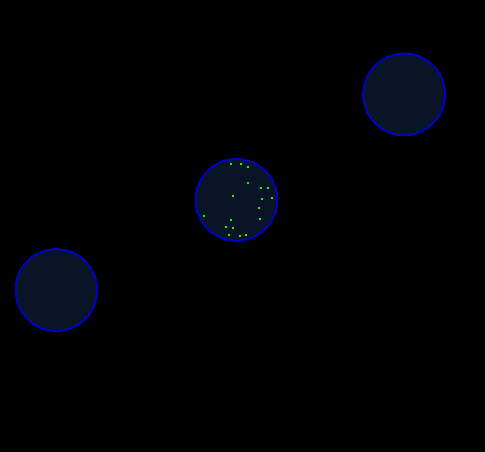
\includegraphics[width=\textwidth]{chapter7/IMG_ch7/Bursting/Basic/basic1} % Adjust the image path as necessary
        \caption{}
        \label{fig:figure1}
    \end{subfigure}
    \hspace{\fill} % Optional: adds space between figures
    \begin{subfigure}{0.48\textwidth}
        \centering
        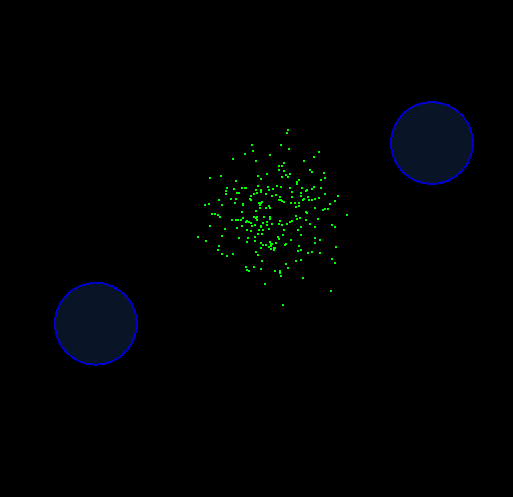
\includegraphics[width=\textwidth]{chapter7/IMG_ch7/Bursting/Basic/basic2} % Adjust the image path as necessary
        \caption{}
        \label{fig:figure2}
    \end{subfigure}

    \vspace{1em} % Small vertical space between rows

    % Second row of two figures
    \begin{subfigure}{0.48\textwidth}
        \centering
        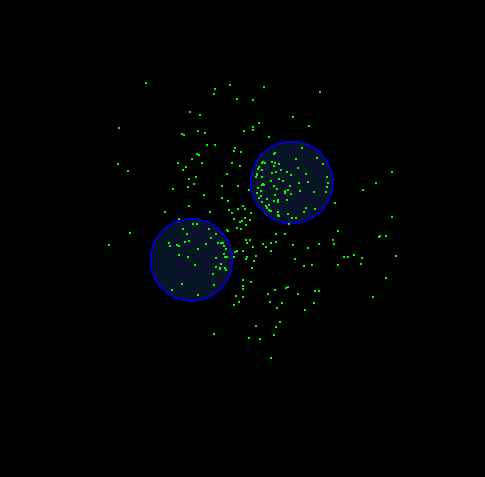
\includegraphics[width=\textwidth]{chapter7/IMG_ch7/Bursting/Basic/basic3} % Adjust the image path as necessary
        \caption{}
        \label{fig:figure3}
    \end{subfigure}
    \hspace{\fill} % Optional: adds space between figures
    \begin{subfigure}{0.48\textwidth}
        \centering
        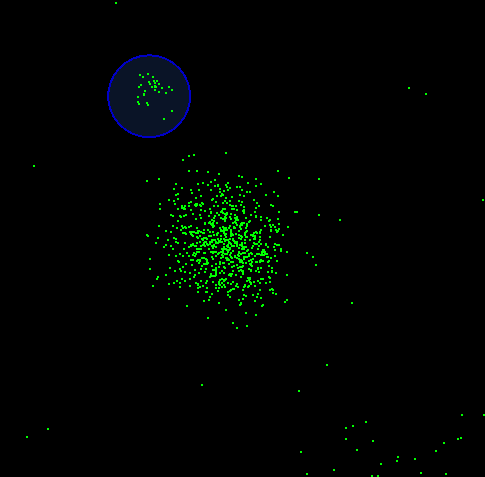
\includegraphics[width=\textwidth]{chapter7/IMG_ch7/Bursting/Basic/basic4} % Adjust the image path as necessary
        \caption{}
        \label{fig:figure4}
    \end{subfigure}

    \caption{(a), Intracellular replication before bursting. (b) Cell bursts, and the contents spans the extracellular space before finding new hosts.  (c) Macrophages are motile. They wander around the extracellular matrix,  phagocytosing debris and extracellular pathogens alike.  (d) A second round of cell bursting is displayed, in this case, the second load is larger.}
    \label{fig:four_figures}
\end{figure}















\subsection*{Three non-basic modifications}
Here we shall seek to describe rigorously the non-extinction probabilities though time of processes with varied initial state that are subject to non-linear dynamics. Basically, a number of replicative units found an infection within a host cell, their dynamics accord with a continuous-time birth death process. What is the probability at time $t$ there is at least one unit still alive, i.e. ``the infection'' has not died out? This will depend on the criticality of the process --- whether a given unit is expected to leave behind greater or less than a replacement of itself --- which will depend on the birth and death rates, $\lambda$ and $\mu$. But we are here interested in the effect of process non-linearities, and what implications these have for survivability at varied initial counts, $\xx_0 = n$.\par

Taking the standard birth-death process, $\xt$, for now with one initial replicative unit, $\xx_0$. Its transition rates are defined
\begin{align*}
\pr{\Delta \xt = 1} &= \lambda \xt \delt + o(\delt),\\
\pr{\Delta \xt = -1} &= \mu \xt \delt + o(\delt),\\
\pr{\Delta \xt = 0} &= 1 - (\lambda + \mu) \xt \delt + o(\delt),
\end{align*}
(with $\Delta \xt = \xdt - \xt$). In this linear-format, the process is said to be critical exactly when $\lambda = \mu$. Each replicative unit eventually dies or divides, so when chances for each of these eventualities balances, the expected number of ``offspring'' for a given unit will be 1. More rigorously, defining the count of progeny units left behind as $Z$:
\begin{align*}
\pr{Z=2} &= \frac{\lambda}{\lambda + \mu}\\
\pr{Z=0} &= \frac{\mu}{\lambda + \mu}
\end{align*}
Left behind should be read as ``following the next event'', so time become irrelevant. When $\lambda = \mu$, 
$$\pr{Z=2} = \pr{Z=0} = \frac{\lambda}{2\lambda} = \frac{1}{2}.$$
And the expected replacement count for a particles is 1;
$$\mean{Z} = 0\cdot \pr{Z = 0} + 2 \cdot \pr{Z = 2} = 2\cdot \frac{1}{2} = 1.$$
If $\lambda > \mu$, this value is greater than 1, and if $\lambda < \mu$, it's less than 1, these cases are termed supercritical and subcritical respectively.
\vspace{15pt}
\begin{adjustwidth}{2cm}{}
\begin{itemize}
\item[$\mean{Z} > 1$:] \textbf{Supercritical}. Given on-average replacement and increase, a population may avoid extinction indefinitely. This occurring with some probability $S(t)$ as defined below. 
\item[$\mean{Z} = 1:$] \textbf{Critical}. Despite each unit fully replacing itself in expectation, a critical birth death chain will inevitably decline to nothing. Interestingly, the expected time until this happens is infinite. 
\item[$\mean{Z} < 1:$] \textbf{Subcritical}. On average, each unit will not replace itself and the process will decline, though stochastically, with ultimate demise --- fixation at 0.
\end{itemize}
\end{adjustwidth}



\subsection{Gompertz Poisson first jump and expected value}
The Poisson process, as $\xt$ is defined
\begin{align*}
\pr{\Delta \xt = 1} &= \lambda \delt + o(\delt),\\
\pr{\Delta \xt = 0} &= 1 - \lambda  \delt + o(\delt);
\end{align*}
a constant rate of stochastic incidence events. 
\subsubsection{First jump probability}
Defining $\pr{\xt = i} = p_i(t)$, the move from state 0 to 1 can be quantified with the state zero probability, $p_0(t)$. And this can be computed in the following way. 
$$p_0(t+\delt) = p_0(t)[1 - \lambda \delt + o(t)].$$
In plain English: the probability $\xdt = 0$ is the likelihood $\xt = 0$, and, in the interval $(t, t + \delt]$, nothing happens. There is no ``immigration'' event. When taken in the limit $\delt\to 0$, this formula derives the ODE, 
$$\frac{p_0(t+\delt) - p_0(t)}{\delt} = \lambda p_0(t)+  o(\delt)$$
$$ \xrightarrow{\underset{\delt \to 0}{}}  \hspace{5pt}  \ddt{p_0(t)} = \lambda p_0(t).$$ 

\noindent
This is simple, of course. And the solution is a basic decaying exponential, $p_0(t) = \ee^{-\lambda t}$. But what would happen if we modified the addition rate, making the process inhomogeneous in time. Say for example the rate itself was a decaying exponential: $\lambda \to \lambda(t) = \ee^{-t}$?  
\begin{align*}
\pr{\Delta \xt = 1} &= \lambda(t) \delt + o(\delt),\\
\pr{\Delta \xt = 0} &= 1 - \lambda(t)  \delt + o(\delt);
\end{align*}
The question is: can we make the same simple derivation of $p_0(t)$ without issue? It's not obvious at first that  everything will work out. When writing the first step equation,
$$p_0(t+\delt) = p_0(t)[1 - \lambda(\mathbf{?}) \delt + o(t)],$$
there is some ambiguity about what should be in the argument of $\lambda(t)$. Do we take the value at the start, or the end of the interval: $\lambda(t)$ or $\lambda(t+\delt)$? The probability that an event happens or not during the interval can not simply be defined by either of these. But in all likelihood, we are confusing ourselves for no reason. Because the equation is ultimately evaluated in the limit, it shouldn't matter. $\lim_{\delt\to0}(t+\delt) = t $, so the two cases end up being identical. It seems obvious when put like this, I just hesitate because things aren't always as they seem in probability theory and we wouldn't want to be caught out. In any case, it is possible and straightforward to verify the subsequent result.\par
With the inhomogeneous version of the equation,
$$\ddt{p_0(t)} = \lambda(t)p_0(t), \hspace{10pt} \lambda(t) = \ee^{-\alpha t},$$
$p_0(t)$ can be computed as
$$p_0(t) = \ee^{\lrb{\ee^{- t} - 1}  }$$  
With $\lambda(t) = \beta \ee^{-\alpha t}$, this generalises to
$$p_0(t) = \ee^{\frac{\beta}{\alpha} \lrb{\ee^{-\alpha t} - 1}  }.$$ 





\def\eval{0.36787}

\begin{figure}[h]
	
    \centering
    \resizebox{0.8\textwidth}{!}{%
    \begin{tikzpicture}
        \begin{axis}[
            xlabel={$t$},
            ylabel={$f(t) = \ee^{\frac{\beta}{\alpha}\lrb{\ee^{-\alpha t}} - 1  }$ with $\beta = \alpha = 1$ },
            axis lines=middle,
            xmin=0, xmax=5.2,
            ymin=0, ymax=1.2,
            width=0.5\textwidth,
            height=0.2\textwidth,
            xtick={0,1,2,3,4,5},
            ytick={0, \eval,1},
            yticklabels={0,$\ee^{-\frac{\beta}{\alpha}}$,1},
            tick label style={font=\scriptsize},
            xlabel style={at={(ticklabel* cs:1)}, anchor=north west, font=\scriptsize},
            ylabel style={at={(ticklabel* cs:1)}, anchor=south west, font=\scriptsize},
            legend style={at={(0.5,1.03)},anchor=south,legend cell align=left,font=\scriptsize},
            ]
            \addplot[blue, domain=0:5.2, samples=100] {exp(exp(-x) - 1)};
            \draw[red, dashed] (axis cs:0,0.367879) -- (axis cs:5.2,0.367879);
        \end{axis}
    \end{tikzpicture}
    }
    \caption{Decaying exponential function $f(t) = e^{{e^{-t}-1}}$.}
    \label{fig:exponential}
\end{figure}



\subsection*{Poisson Gompertz}

\begin{align*}
\pr{\Delta \xt = 1} &= \lambda(t) \delt + o(\delt),\\
\pr{\Delta \xt = 0} &= 1 - \lambda(t)  \delt + o(\delt);
\end{align*}



\subsubsection*{No added constant}

$\lambda(t) = \beta \ee^{-\alpha t}$
$$\mean{\xt} = \frac{\beta}{\alpha} \lrb{1 - \ee^{-\alpha t}}$$
$$p_0(t) = \ee^{\frac{\beta}{\alpha} \lrb{\ee^{-\alpha t} - 1}  }.$$ 


\subsubsection*{Added constant}

$\lambda(t) = \beta \ee^{-\alpha t} + \gamma$


$$\mean{\xt} = \frac{\beta}{\alpha} \lrb{1 - \ee^{-\alpha t}} + \gamma t$$



\subsection*{Deterministic version}

Considering a single unit exhibiting Gompertz activation.\par

\vspace{5pt}

\noindent
$N(t)$: activation of a node.
$$\ddt{N(t)} = \lrb{\lambda(t) - \mu} N(t)$$
\begin{itemize}
\item Gompertz growth rate: $\lambda(t) = \beta \ee^{-\alpha t} + \gamma$. Made up of,
\begin{itemize}
\item $\beta \ee^{-\alpha t}$: decaying term represents the reduced proliferation in response to recognition and desired ceasing, and
\item $\gamma$: constant, a sort of base-line growth rate. 
\end{itemize}
\item $\mu$: decline rate.
\end{itemize}
Formula: 
$$N(t) = N_0 \ee^{\lrbs{\frac{\beta}{\alpha} \lrb{1 - \ee^{-\alpha t} } + (\gamma - \mu) t }  }$$
Interesting case: When $\mu > \gamma$ and $\mu < \gamma + \beta \ee^{-\alpha t}$ when t = 0. Sufficient to say $\gamma < \mu < \gamma + \beta$.











































%%%%%%%%%%%%%%%%%%%%%%%%%%%%%%%%%%%%%%%%%%%%%%%%%%%%%%%%%%%%%%%%%%%%%%%%%%%%%%%%%%%%%%%%%%%%%%%%%%%%%%%%%%%5

\section{Replicator suppressor}







\definecolor{Rec}{HTML}{008000}
\definecolor{Rup}{HTML}{992600}
\definecolor{gray1}{HTML}{d9d9d9}%{cccccc}
\definecolor{na1}{HTML}{4d94ff}
\definecolor{nb1}{HTML}{d6b129}
\definecolor{mut1}{HTML}{80d5d5}
\definecolor{Rec2}{HTML}{40bf40}
\definecolor{Rup2}{HTML}{c67053}
\definecolor{blu}{HTML}{002266}



% Define custom colors that match the colors in the provided image
\definecolor{spyder5keyword}{rgb}{0.15, 0.15, 0.7}   % Orange for keywords
\definecolor{spyder5comment}{rgb}{0.25, 0.50, 0.37}  % Greenish for comments
\definecolor{spyder5string}{rgb}{0.56, 0.0, 0.56}    % Purple for strings
\definecolor{spyder5number}{rgb}{0.19, 0.55, 0.91}   % Light blue for numbers
\definecolor{spyder5identifier}{rgb}{0.81, 0.85, 0.87} % Light gray for identifiers
\definecolor{spyder5background}{rgb}{0.97, 0.97, 0.9} % Dark gray for background
\definecolor{spyder5text}{rgb}{0, 0, 0}        % White for text

% Configure the listings package to use these colors
\lstset{
    backgroundcolor=\color{spyder5background},   
    basicstyle=\ttfamily\small\color{spyder5text},
    keywordstyle=\color{spyder5keyword}\bfseries,
    commentstyle=\color{spyder5comment}\itshape,
    stringstyle=\color{spyder5string},
    numberstyle=\color{spyder5number},
    identifierstyle=\color{spyder5text},
    showstringspaces=false,
   numbers=right,
    numbersep=5pt,
    tabsize=4,
    breaklines=true,
    frame=single,
    captionpos=b,
   framexleftmargin=10pt,  % Add space to the left inside the box
    %framexrightmargin=10pt, % Add space to the right inside the box
    %xleftmargin=10pt,       % Indent the whole box
    %xrightmargin=10pt       % Add space to the right outside the box
}









\begin{figure}[H]
    \centering
    % First row of two figures
    \begin{subfigure}{0.48\textwidth}
        \centering
        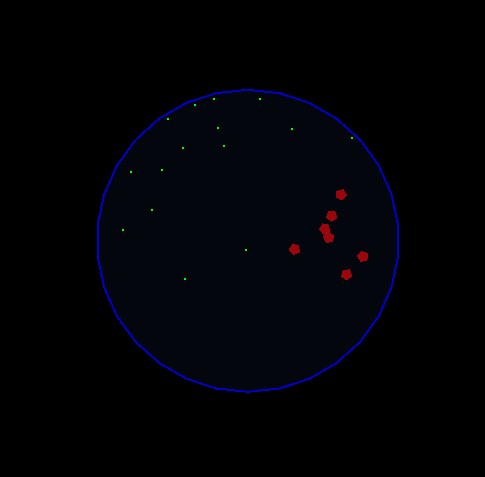
\includegraphics[width=\textwidth]{chapter7/IMG_ch7/Bursting/RS/RS1} % Adjust the image path as necessary
        \caption{}
        \label{fig:figure1}
    \end{subfigure}
    \hspace{\fill} % Optional: adds space between figures
    \begin{subfigure}{0.48\textwidth}
        \centering
        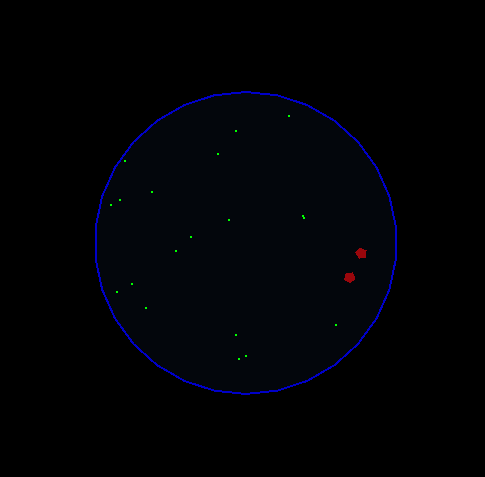
\includegraphics[width=\textwidth]{chapter7/IMG_ch7/Bursting/RS/RS2} % Adjust the image path as necessary
        \caption{}
        \label{fig:figure2}
    \end{subfigure}


    \caption{(a), Intracellular granules are represented in red, pathogenic particles in green. In this simulation,  when one of each contacts, they anniahilate. (b), the pathogen has replicated and appears to be overcoming the immune challenge of the granules. }
    \label{fig:four_figures}
\end{figure}


\subsection{Model definition}


Both macrophages and neutrophils contain small a number of small packets called granules. These contain oxidative chemicals and are used to kill engulfed pathogen. Neutrophils are of the category ``granulocyte'' and as the name suggests contain a larger number of these packets than macrophages. 

When a count of pathogenic units enters a macrophage by phagocytosis, they begin to face the the action of these granules. Given the packets are finite in number and depletable, it might be that a larger incident cohort of replicators has a greater chance of eventual survival. 

Here we explore a simple model which represents the interplay between the two opposing forces. Replicative pathogenic particles fighting for survival against its host cell's inbuilt defence mechanism. The model thus constitutes two unit types: $\xt$ represents the infectious agents, $\yt$ refers to the remaining number of within-cell granules. From a defined initial condition ($\xx_0, \yy_0$), the dynamic between these two factors results in either pathogen extinction, or the overthrowing of immunity resulting in unbounded growth in $\xt$. Of course, in reality growth will not be truly without limit. Intracellular capacity will eventually introduce a threshold to further expansion without cell bursting.\par
Dynamic transitions are defined quite simple. Units of $\xt$ will divide and increase according to the standard mechanism seen in a birth process. 
$$\pr{\Delta \xt = 1, \Delta \yt = 0} = \lambda \xt \Delta t + o(\Delta t) $$
Suppressive interactions occur with a rate proportional to the product of the two counts, and result in a single elimination of each type.  
 $$\pr{\Delta \xt = -1, \Delta \yt = -1} = \alpha \xt \yt  \Delta t + o(\Delta t) $$
 Hence, with just the addition of a no-event possibility, 
 $$\pr{\Delta \xt = 0, \Delta \yt = 0} = 1 -  \lrb{ \lambda\xt   + \alpha \xt \yt } \Delta t + o(\Delta t) $$
 the continuous time Markov chain is fully defined over infinitesimal durations.


Our focus of interest is in understanding the relationship between incident pathogen count and infection survivability. In other words the probability 
$$\pr{\text{infection survival}} =  1 - \lim_{t\to\infty} \pr{\xt = 0},$$
signifying late time non-extinction. Cases where survival ultimately persists will include the complete exhaustion of antagonistic granules ($\yt = 0$). One may devise a model in which the granules are produced at some rate by the cell, but for now we will aim to understand this more simple version where an initial immune capacity is fixed ($\yy_0$) and never supplemented.  
























\subsection{Mathematical definition}


CT Markov process,
$$\mathcal{X} = \{ (\xt, \yt): t\geq 0\},$$
 state space.

$$\mathcal{S} = \{    (i,j)\;\; |\;\; i \in \mathbb{N} \cup \{0\}  ,\;\;j\in\{0,\dots,N\}\} .$$








\begin{figure}[H]\label{grid}
\begin{center}
\begin{tikzpicture}[scale=0.8]
% axis and labels 
\draw[thick, dashed] (0,0)--(7.7,0) node[below, yshift=-15pt, xshift=-55pt]{$\xt:$ \small Replicators};
\draw[thick, dashed] (0,0)--(0,4.7) node[left, xshift=-15pt, yshift=-55pt]{$\yt:$} node[left, xshift=-15pt, yshift=-65pt]{\small Granules};
% Grey circles
\foreach \x in {1,2,3,4,5,6,7}
\foreach \y in {1,2,3,4}
\draw[fill = gray1] (\x,\y) circle (3.5pt);
 
 % Axis ticks
\foreach \x in {0,1,2,3,4,5,6,7}
\draw (\x,0) node[below, yshift=-4.5pt]{\small\x} ;
\foreach \y in {0,1,2,3,4}
\draw (0,\y) node[left, xshift=-4.5pt]{\small\y} ;

% Green and red circles
\foreach \x in {1,2,3,4,5,6,7}
\draw[fill = Rec2] (\x, 0) circle (3.6pt);

\foreach \y in {0,1,2,3,4,}
\draw[fill = Rup2] (0, \y) circle (3.6pt);

% Bold transitions diagonal
\foreach \x in {0,1,2,3,4,5,6}
\foreach \y in {1,2,3,4}
{\draw[thick, ->, mut1, >=stealth] (\x+0.8, \y-0.2) -- (\x + 0.2, \y-0.8);}

% Bold horizontal transitions 
\foreach \x in {1,2,3,4,5,6}
\foreach \y in {0,1,2,3,4}
{\draw[>=stealth, ->,thick, na1] (\x+0.2, \y) -- (\x+0.8, \y);}

% Opacity transitions
\foreach \x in {7}
\foreach \y in {0,1,2,3,4}
{\draw[>=stealth, ->,thick, na1, opacity = 0.2] (\x+0.2, \y) -- (\x+0.8, \y);}

\foreach \y in {1,2,3,4}
{\draw[>=stealth, ->,thick, mut1, opacity = 0.3] (7+0.8, \y-0.2) -- (7 + 0.2, \y-0.8);}


\end{tikzpicture}
\end{center}
\caption{State space $\mathcal{S}$ with Ruptured state $R$ in red on the right; green recovery state is seen at (0,0). Arrows show possible transitions between states: \textbf{\textcolor{na1}{blue}} for births and deaths of bacteria type $a$, those of type $b$ are represented by \textbf{\textcolor{nb1}{orange}}, \textbf{\textcolor{mut1}{cyan}} for differentiations from type $a$ to $b$, and \textbf{\textcolor{Rup2}{red}} for the macrophage rupture event.}
\label{grid}
\end{figure}












\begin{figure}[H]\label{grid}
\begin{center}
\begin{tikzpicture}[scale=0.8]
% axis and labels 
\draw[thick, dashed] (0,0)--(7.7,0) node[below, yshift=-15pt, xshift=-55pt]{$\xt:$ \small Replicators};
\draw[thick, dashed] (0,0)--(0,4.7) node[left, xshift=-15pt, yshift=-55pt]{$\yt:$} node[left, xshift=-15pt, yshift=-65pt]{\small Granules};
% Grey circles
\foreach \x in {1,2,3,4,5,6,7}
\foreach \y in {1,2,3,4}
\draw[fill = gray1] (\x,\y) circle (3.5pt);
 
 % Axis ticks
\foreach \x in {0,1,2,3,4,5,6,7}
\draw (\x,0) node[below, yshift=-4.5pt]{\small\x} ;
\foreach \y in {0,1,2,3,4}
\draw (0,\y) node[left, xshift=-4.5pt]{\small\y} ;

% Green and red circles
\foreach \x in {1,2,3,4,5,6,7}
\draw[fill = Rec2] (\x, 0) circle (3.6pt);

\foreach \y in {0,1,2,3,4,}
\draw[fill = Rup2] (0, \y) circle (3.6pt);

% Bold transitions diagonal
\foreach \x in {0,1,2,3,4,5,6}
\foreach \y in {1,2,3,4}
{\draw[thick, ->, mut1, >=stealth] (\x+0.8, \y-0.2) -- (\x + 0.2, \y-0.8);}

% Bold horizontal transitions 
\foreach \x in {1,2,3,4,5,6}
\foreach \y in {0,1,2,3,4}
{\draw[>=stealth, ->,thick, na1] (\x+0.2, \y) -- (\x+0.8, \y);}

% Opacity transitions
\foreach \x in {7}
\foreach \y in {0,1,2,3,4}
{\draw[>=stealth, ->,thick, na1, opacity = 0.2] (\x+0.2, \y) -- (\x+0.8, \y);}

\foreach \y in {1,2,3,4}
{\draw[>=stealth, ->,thick, mut1, opacity = 0.3] (7+0.8, \y-0.2) -- (7 + 0.2, \y-0.8);}


\end{tikzpicture}
\end{center}

\label{grid}
\end{figure}


\vspace{5pt}
\noindent









\begin{figure}[H]\label{grid}
\begin{center}
\begin{tikzpicture}[scale=0.6]
% axis and labels 
\draw[thick, dashed] (0,0)--(9.7,0) node[below, yshift=-15pt, xshift=-55pt]{$\xt:$ \small Replicators};
\draw[thick, dashed] (0,0)--(0,6.7) node[left, xshift=-15pt, yshift=-55pt]{$\yt:$} node[left, xshift=-15pt, yshift=-65pt]{\small Granules};
% Grey circles
\foreach \x in {1,2,3,4,5,6,7,8}
\foreach \y in {1,2,3,4,5,6}
\draw[fill = gray1] (\x,\y) circle (3.5pt);

% Grey circles
\foreach \x in {9}
\foreach \y in {1,2,3,4,5,6}
\draw  (\x,\y)node[]{\small$\cdots$};
 
 
 % Axis ticks
\foreach \x in {0,1,2,3,4,5,6,7,8,9}
\draw (\x,0) node[below, yshift=-4.5pt]{\small\x} ;
\foreach \y in {0,1,2,3,4,5,6}
\draw (0,\y) node[left, xshift=-4.5pt]{\small\y} ;

% Green and red circles
\foreach \x in {1,2,3,4,5,6,7,8,9}
\draw[fill = Rec2] (\x, 0) circle (3.5pt);

\foreach \y in {0,1,2,3,4,5,6}
\draw[fill = Rup2] (0, \y) circle (3.5pt);

% Shaded triangle with rounded corners
\fill[fill=nb1, rounded corners=10pt, opacity = 0.5] 
(0.6,6.5) -- (6.9,6.5) -- (0.6,0.1) -- cycle;


\fill[fill=Rec2, rounded corners=7pt, opacity = 0.5] 
(0.3,-0.3) -- (7,6.5) -- (9.7,6.5) -- (9.7, -0.3) -- cycle;

\fill[fill=Rup2, rounded corners=6pt, opacity = 0.5] 
(0.54,-0.3) -- (-0.4,-0.3) -- (-0.4,6.5) -- (0.54,6.5) -- cycle;


\end{tikzpicture}
\end{center}

\label{grid}
\end{figure}









\begin{figure}[H]\label{grid}
\begin{center}
\begin{tikzpicture}[scale=0.7]
% axis and labels 
\draw[thick, dashed] (0,0)--(8.2,0) node[below, yshift=-15pt, xshift=-55pt]{$\xt:$ \small Replicators};
\draw[thick, dashed] (0,0)--(0,6.7) node[left, xshift=-15pt, yshift=-55pt]{$\yt:$} node[left, xshift=-15pt, yshift=-65pt]{\small Granules};
% Grey circles
\foreach \x in {1,2,3,4,5,6,7}
\foreach \y in {1,2,3,4,5,6}
\draw[fill = gray1] (\x,\y) circle (3.5pt);

% Grey circles
\foreach \x in {8}
\foreach \y in {1,2,3,4,5,6}
\draw  (\x,\y)node[]{\small$\cdots$};
 
 % Axis ticks
\foreach \x in {0,1,2,3,4,5,6,7}
\draw (\x,0) node[below, yshift=-4.5pt]{\small\x} ;
\foreach \y in {0,1,2,3,4,5,6}
\draw (0,\y) node[left, xshift=-4.5pt]{\small\y} ;

% Green and red circles
\foreach \x in {1,2,3,4,5,6,7}
\draw[fill = Rec2] (\x, 0) circle (3.5pt);

\foreach \y in {0,1,2,3,4,5,6}
\draw[fill = Rup2] (0, \y) circle (3.5pt);


\filldraw[blue,rounded corners = 1mm, opacity = 0.2]
let \p1=($(1,1)!-2mm!(6,6)$),
\p2=($(6,6)!-2mm!(0,0)$),
\p3=($(\p1)!2mm!90:(\p2)$),
\p4=($(\p1)!2mm!-90:(\p2)$),
\p5=($(\p2)!2mm!90:(\p1)$),
\p6=($(\p2)!2mm!-90:(\p1)$)
in
(\p3) -- (\p4)-- (\p5) -- (\p6) -- cycle;

\filldraw[blue,rounded corners = 1mm, opacity = 0.2]
let \p1=($(1,2)!-2mm!(5,6)$),
\p2=($(5,6)!-2mm!(0,1)$),
\p3=($(\p1)!2mm!90:(\p2)$),
\p4=($(\p1)!2mm!-90:(\p2)$),
\p5=($(\p2)!2mm!90:(\p1)$),
\p6=($(\p2)!2mm!-90:(\p1)$)
in
(\p3) -- (\p4)-- (\p5) -- (\p6) -- cycle;

\filldraw[blue,rounded corners = 1mm, opacity = 0.2]
let \p1=($(1,3)!-2mm!(4,6)$),
\p2=($(4,6)!-2mm!(0,2)$),
\p3=($(\p1)!2mm!90:(\p2)$),
\p4=($(\p1)!2mm!-90:(\p2)$),
\p5=($(\p2)!2mm!90:(\p1)$),
\p6=($(\p2)!2mm!-90:(\p1)$)
in
(\p3) -- (\p4)-- (\p5) -- (\p6) -- cycle;

\filldraw[blue,rounded corners = 1mm, opacity = 0.2]
let \p1=($(1,4)!-2mm!(3,6)$),
\p2=($(3,6)!-2mm!(0,3)$),
\p3=($(\p1)!2mm!90:(\p2)$),
\p4=($(\p1)!2mm!-90:(\p2)$),
\p5=($(\p2)!2mm!90:(\p1)$),
\p6=($(\p2)!2mm!-90:(\p1)$)
in
(\p3) -- (\p4)-- (\p5) -- (\p6) -- cycle;

\filldraw[blue,rounded corners = 1mm, opacity = 0.2]
let \p1=($(1,5)!-2mm!(2,6)$),
\p2=($(2,6)!-2mm!(0,4)$),
\p3=($(\p1)!2mm!90:(\p2)$),
\p4=($(\p1)!2mm!-90:(\p2)$),
\p5=($(\p2)!2mm!90:(\p1)$),
\p6=($(\p2)!2mm!-90:(\p1)$)
in
(\p3) -- (\p4)-- (\p5) -- (\p6) -- cycle;

\filldraw[blue,rounded corners = 1mm, opacity = 0.2]
let \p1=($(1,6)!-2mm!(1,6)$),
\p2=($(1,6)!-2mm!(1,1)$),
\p3=($(\p1)!2mm!90:(\p2)$),
\p4=($(\p1)!2mm!-90:(\p2)$),
\p5=($(\p2)!2mm!90:(\p1)$),
\p6=($(\p2)!2mm!-90:(\p1)$)
in
(\p3) -- (\p4)-- (\p5) -- (\p6) -- cycle;

    % Place text along the line
    \path (1,1) -- (2,2) node[midway, above, sloped, yshift = -5pt] {\tiny  \textbf{\textcolor{blu}{level 1}} };
    \path (1,2) -- (2,3) node[midway, above, sloped, yshift = -5pt] {\tiny  \textbf{\textcolor{blu}{level 2}} };
    \path (1,3) -- (2,4) node[midway, above, sloped, yshift = -5pt] {\tiny  \textbf{\textcolor{blu}{level 3}} };
    \path (1,4) -- (2,5) node[midway, above, sloped, yshift = -5pt] {\tiny  \textbf{\textcolor{blu}{level 4}} };
    \path (1,5) -- (2,6) node[midway, above, sloped, yshift = -5pt] {\tiny  \textbf{\textcolor{blu}{level 5}} };



\end{tikzpicture}
\end{center}

\label{grid}
\end{figure}


















\noindent
We can define the process by its 1 step transition probabilities,
$$p_{(i,j)\to\underbar x}(\Delta t) = \pr{\xdt = \underbar x | \xt = (i,j) },$$
for states $(n_a,n_b),x \in \mathcal{S}$. Considering each of the various steps that can be taken from an arbitrary state ($n_a, n_b$) these are as follows.
\begin{equation*}
p_{(i, j)\to\underbar x}(\Delta t) =
\begin{cases}
\alpha_i\Delta t + o(\Delta t)& \underbar x = (i+1,j)\\
\beta_{i,j}\Delta t + o(\Delta t)& \underbar x = (i-1,j-1)\\
1 - (\alpha_i + \beta_{i,j}) \Delta t + o(\Delta t)& \underbar x = (i,j)
\end{cases}
\end{equation*}
(for $\Delta t \rightarrow 0$).


probability of fixation in set ($\xt = 0$, $\yt$) 
$$\theta_{i,j}$$


$$\theta_{i, j} = \hat \alpha_{i,j} \cdot\theta_{i + 1, j} +  \hat \beta_{i,j}  \cdot\theta_{i - 1, j - 1} $$


$$ \hat \alpha_{i,j} = \frac{ \alpha_i }{\alpha_i + \beta_{i,j}} $$
$$ \hat \beta_{i,j} = \frac{ \beta_{i,j} }{\alpha_i + \beta_{i,j}} $$



 first step analysis matrix equation, $\mathbf{p}^{(0)} = \mathbf{A} \cdot \mathbf{p}^{(0)} + \mathbf{c}$


$$
\scriptsize
\begingroup
\renewcommand*{\arraystretch}{1.45}
\begin{bmatrix}
\theta_{1, 1} \\
\theta_{2,2} \\
\theta_{3,3} \\
\theta_{4,4} \\
\theta_{5,5} \\
\theta_{1,2} \\
\theta_{2,3} \\
\theta_{3,4} \\
\theta_{4,5} \\
\theta_{1,3} \\
\theta_{2,4} \\
\theta_{3,5} \\
\theta_{1,4} \\
\theta_{2,5} \\
\theta_{1,5} 
\end{bmatrix}
\endgroup
=
\left[
\renewcommand*{\arraystretch}{1.45} % Adjust this number to increase or decrease row spacing
\begin{array}{ccccc|cccc|ccc|cc|c}
0 & 0 & 0 & 0 & 0 &   0 & 0 & 0 & 0 &   0 & 0 & 0 &   0 & 0 &   0 \vphantom{\frac{1}{2}}\\
\hat \beta_{2,2} & 0 & 0 & 0 & 0 &   0 & 0 & 0 & 0 &   0 & 0 & 0 &   0 & 0 &   0\vphantom{\frac{1}{2}}\\
0 & \hat \beta_{3,3}  & 0 & 0 & 0 &   0 & 0 & 0 & 0 &   0 & 0 & 0 &   0 & 0 &   0\\
0 & 0 & \hat \beta_{4,4}  & 0 & 0 &   0 & 0 & 0 & 0 &   0 & 0 & 0 &   0 & 0 &   0\\
0 & 0 & 0 & \hat \beta_{5,5}  & 0 &   0 & 0 & 0 & 0 &   0 & 0 & 0 &   0 & 0 &   0\\
\hline
0 & \hat\alpha_{1,2} & 0 & 0 & 0 &   0 & 0 & 0 & 0 &   0 & 0 & 0 &   0 & 0 &   0\\
0 & 0 & \hat\alpha_{2,3} & 0 & 0 &   \hat \beta_{2,3}  & 0 & 0 & 0 &   0 & 0 & 0 &   0 & 0 &   0\\
0 & 0 & 0 & \hat\alpha_{3,4} & 0 &   0 & \hat \beta_{3,4}  & 0 & 0 &   0 & 0 & 0 &   0 & 0 &   0\\
0 & 0 & 0 & 0 & \hat\alpha_{4,5} &   0 & 0 & \hat \beta_{4,5}  & 0 &   0 & 0 & 0 &   0 & 0 &   0\\
\hline
0 & 0 & 0 & 0 & 0 &   0 & \hat\alpha_{1,3} & 0 & 0 &   0 & 0 & 0 &   0 & 0 &   0\\
0 & 0 & 0 & 0 & 0 &   0 & 0 & \hat\alpha_{2,4} & 0 &   \hat \beta_{2,4}  & 0 & 0 &   0 & 0 &   0\\
0 & 0 & 0 & 0 & 0 &   0 & 0 & 0 & \hat\alpha_{3,5} &   0 & \hat \beta_{3,5}  & 0 &   0 & 0 &   0\\
\hline
0 & 0 & 0 & 0 & 0 &   0 & 0 & 0 & 0 &   0 & \hat\alpha_{1,4} & 0 &   0 & 0 &   0\\
0 & 0 & 0 & 0 & 0 &   0 & 0 & 0 & 0 &   0 & 0 & \hat\alpha_{2,5} &   \hat \beta_{2,5}  & 0 &   0\\
\hline
0 & 0 & 0 & 0 & 0 &   0 & 0 & 0 & 0 &   0 & 0 & 0 &   0 & \hat\alpha_{1,5} &   0\\

\end{array}
\right]
\begingroup
\renewcommand*{\arraystretch}{1.45}
\begin{bmatrix}
\theta_{1, 1} \\
\theta_{2,2} \\
\theta_{3,3} \\
\theta_{4,4} \\
\theta_{5,5} \\
\theta_{1,2} \\
\theta_{2,3} \\
\theta_{3,4} \\
\theta_{4,5} \\
\theta_{1,3} \\
\theta_{2,4} \\
\theta_{3,5} \\
\theta_{1,4} \\
\theta_{2,5} \\
\theta_{1,5} 
\end{bmatrix}
\endgroup
+
\begingroup
\renewcommand*{\arraystretch}{1.45}
\begin{bmatrix}
\hat \beta_{1,1} \\
0 \\
0 \\
0 \\
0 \\
\hat \beta_{1,2} \\
0 \\
0 \\
0 \\
\hat \beta_{1,3} \\
0 \\
0 \\
\hat \beta_{1,4} \\
0 \\
\hat \beta_{1,5} \\
\end{bmatrix}.
\endgroup
$$













\begin{figure}[H]
    \centering
    \begin{minipage}{0.3\textwidth}
        \centering
        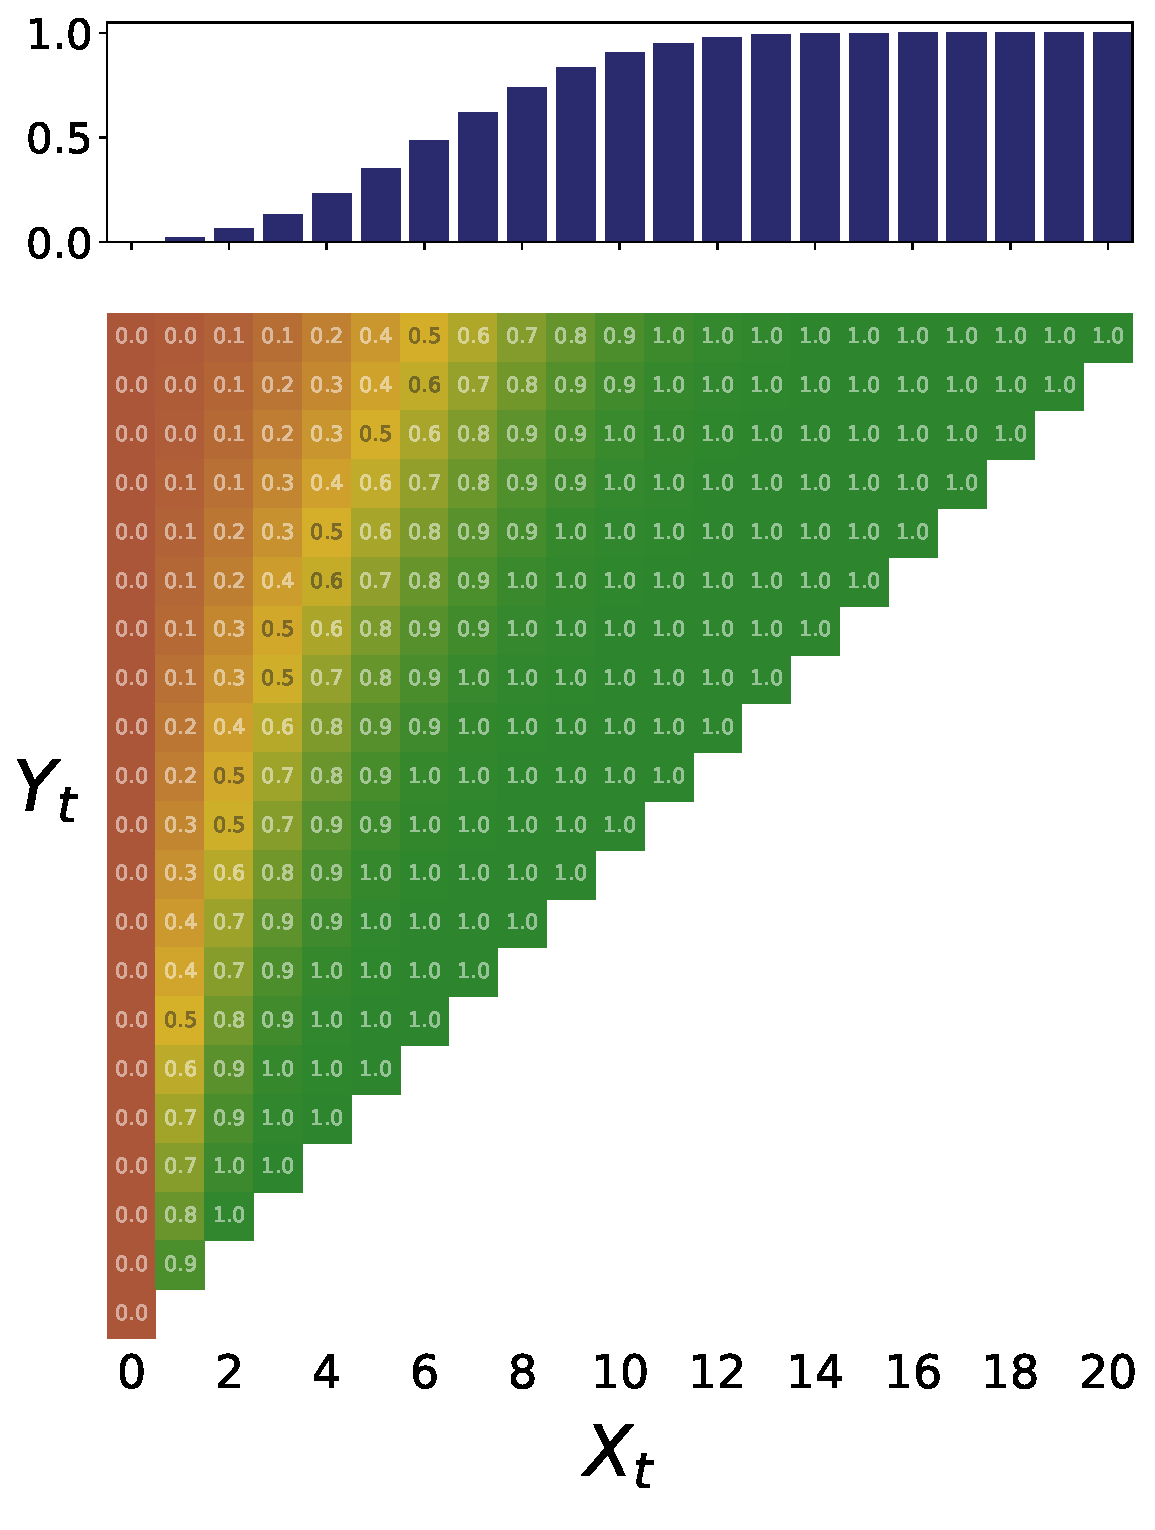
\includegraphics[width=1.1\textwidth]{chapter7/IMG_ch7/RepSupp_20_0.1_1_NBA_.pdf}
    
        \label{fig:graph1}
    \end{minipage}\hfill
    \begin{minipage}{0.3\textwidth}
        \centering
        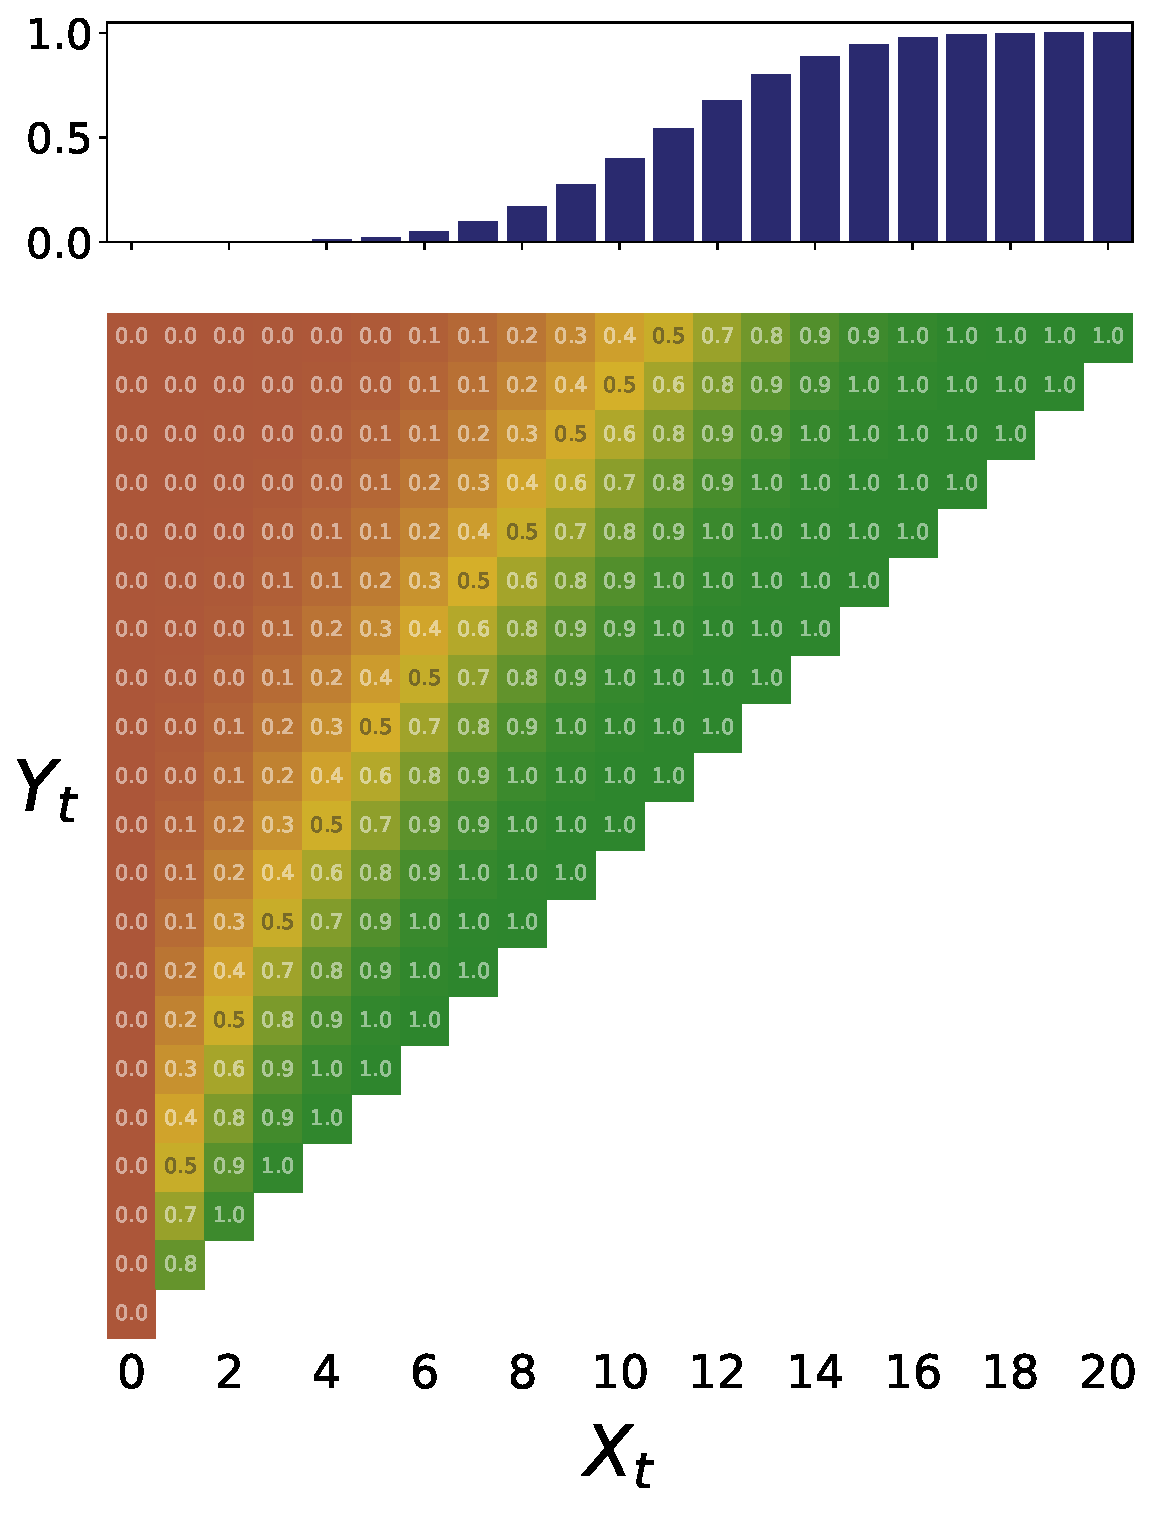
\includegraphics[width=1.1\textwidth]{chapter7/IMG_ch7/RepSupp_20_0.2_1_NBA_.pdf}
  
        \label{fig:graph2}
    \end{minipage}\hfill
    \begin{minipage}{0.3\textwidth}
        \centering
       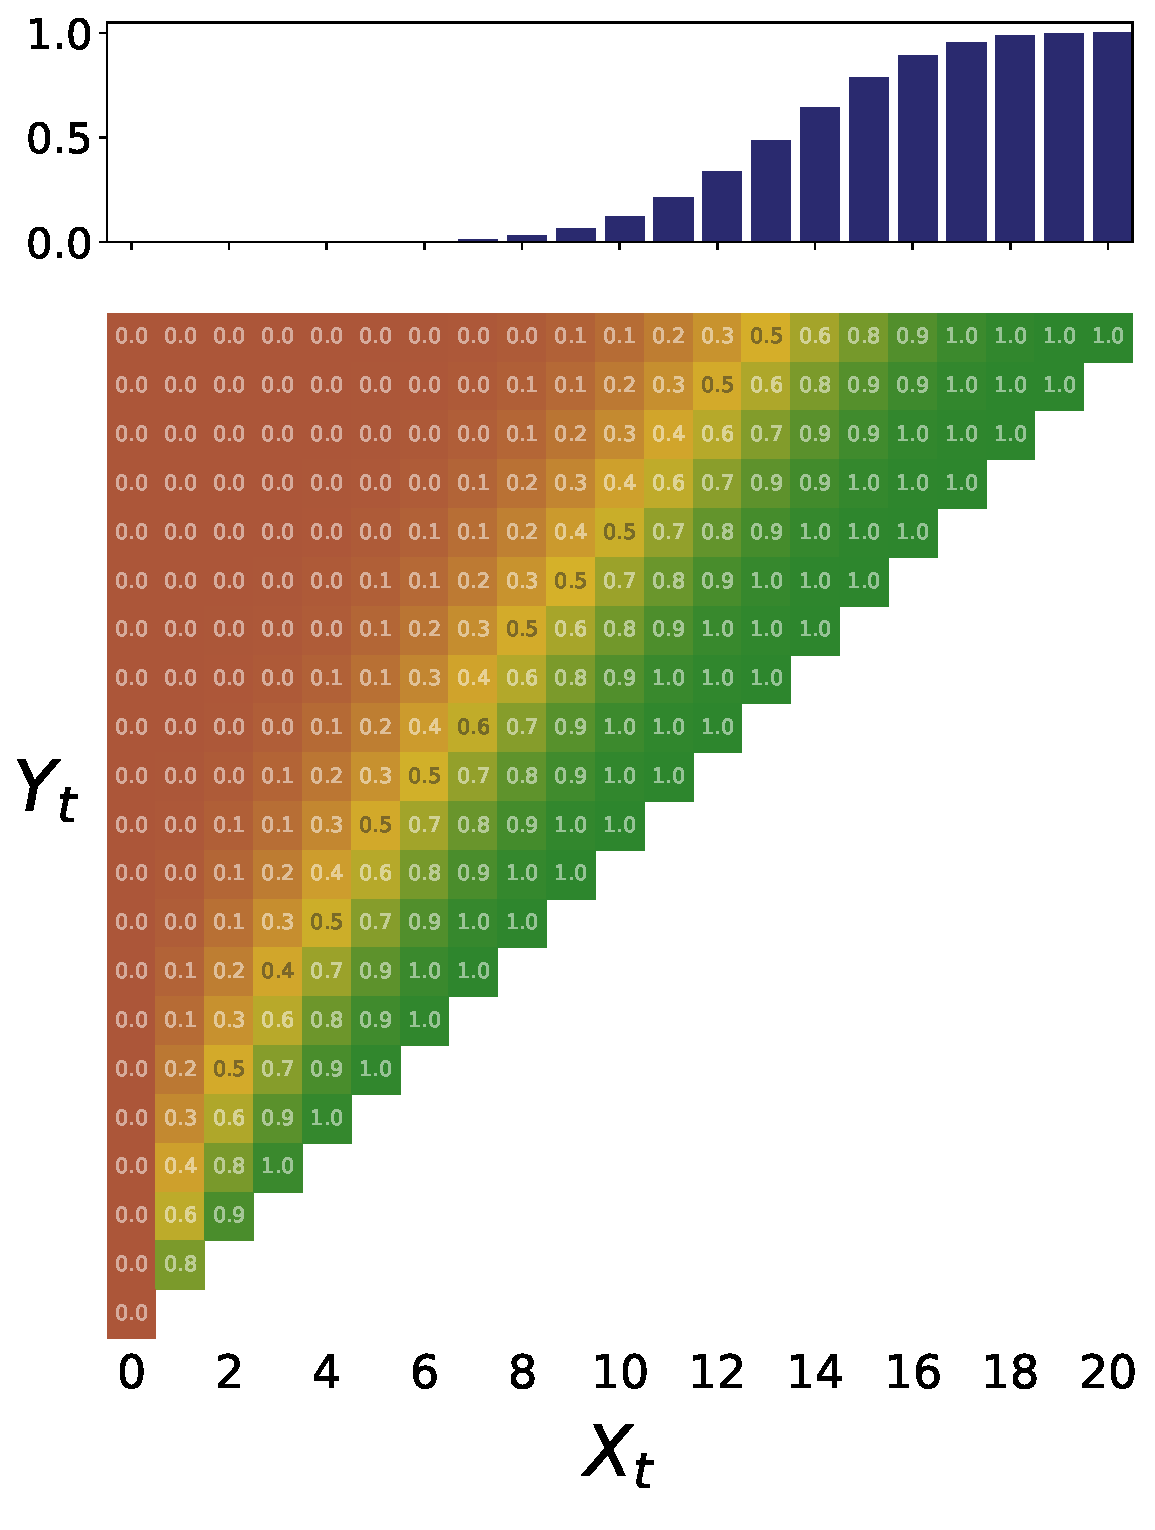
\includegraphics[width=1.1\textwidth]{chapter7/IMG_ch7/RepSupp_20_0.3_1_NBA_.pdf}
    
        \label{fig:graph3}
    \end{minipage}
    \caption{Probabilities of infection survival given initial count of pathogen ($\xt$), and granules ($\yt$).}
    \label{fig:threegraphs}
\end{figure}








\begin{figure}[h!]
    \centering
    \begin{minipage}{0.3\textwidth}
        \centering
        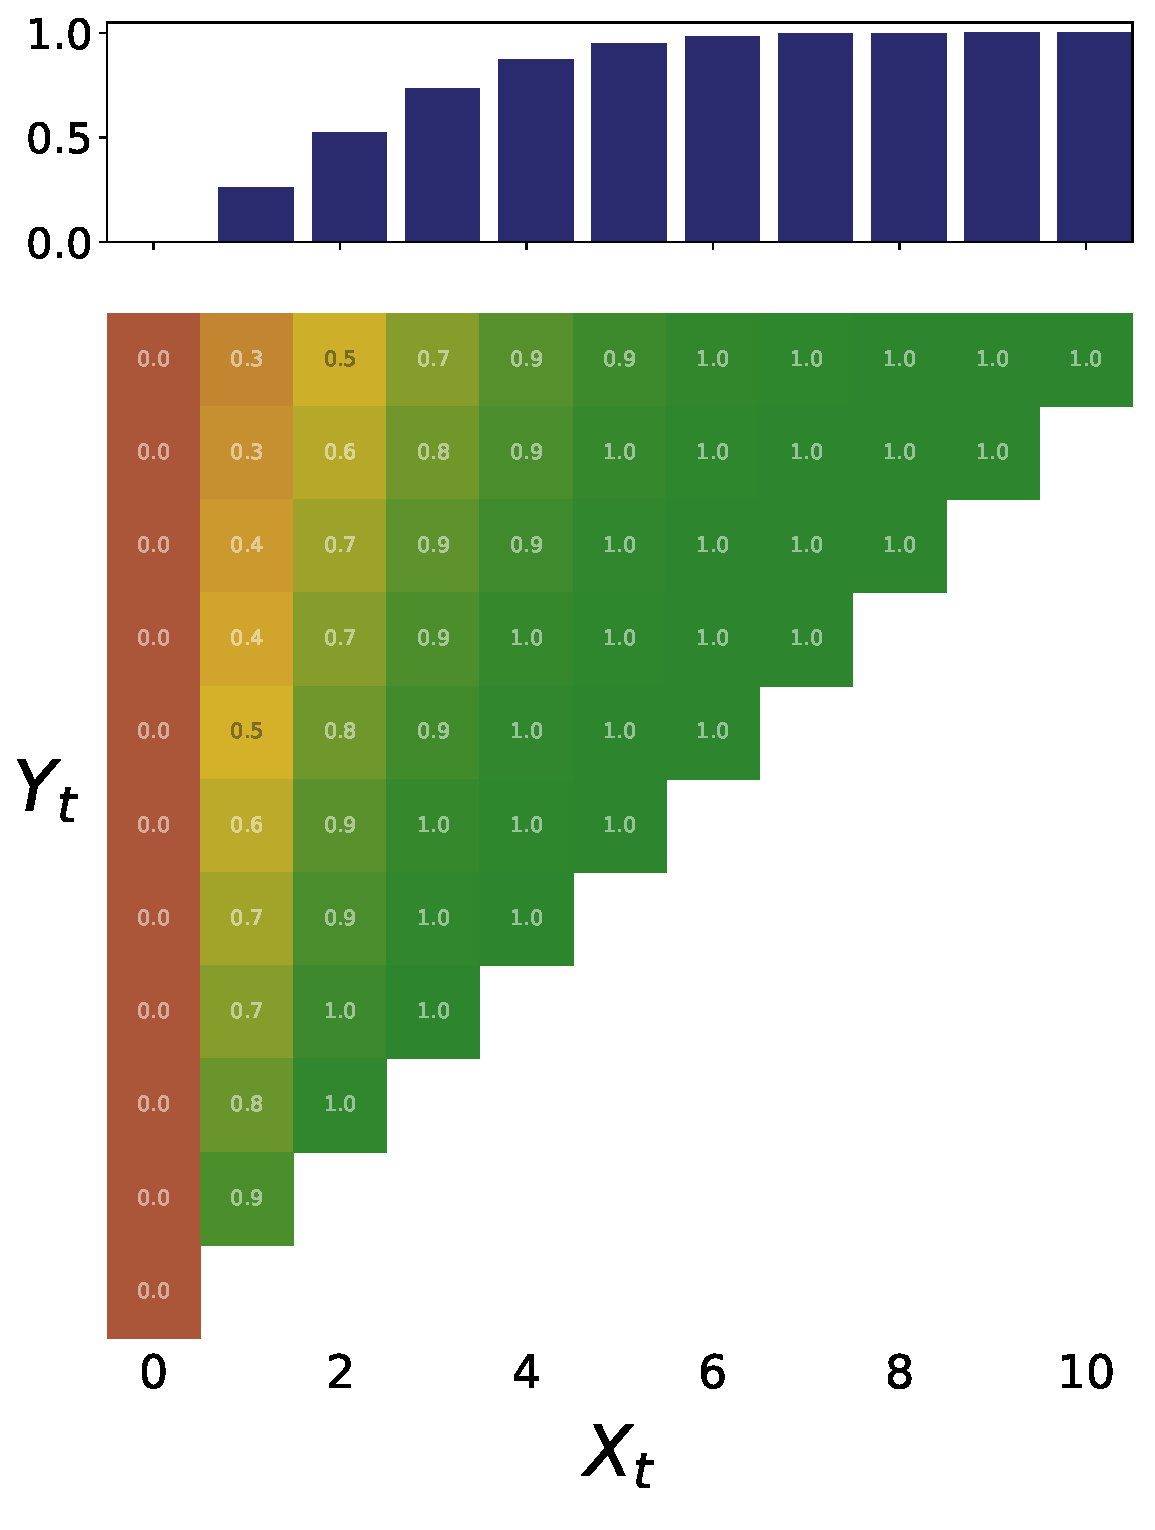
\includegraphics[width=\textwidth]{chapter7/IMG_ch7/RepSupp_10_0.1_1_NBA_.pdf}
        \label{fig:graph1}
    \end{minipage}\hfill
    \begin{minipage}{0.3\textwidth}
        \centering
        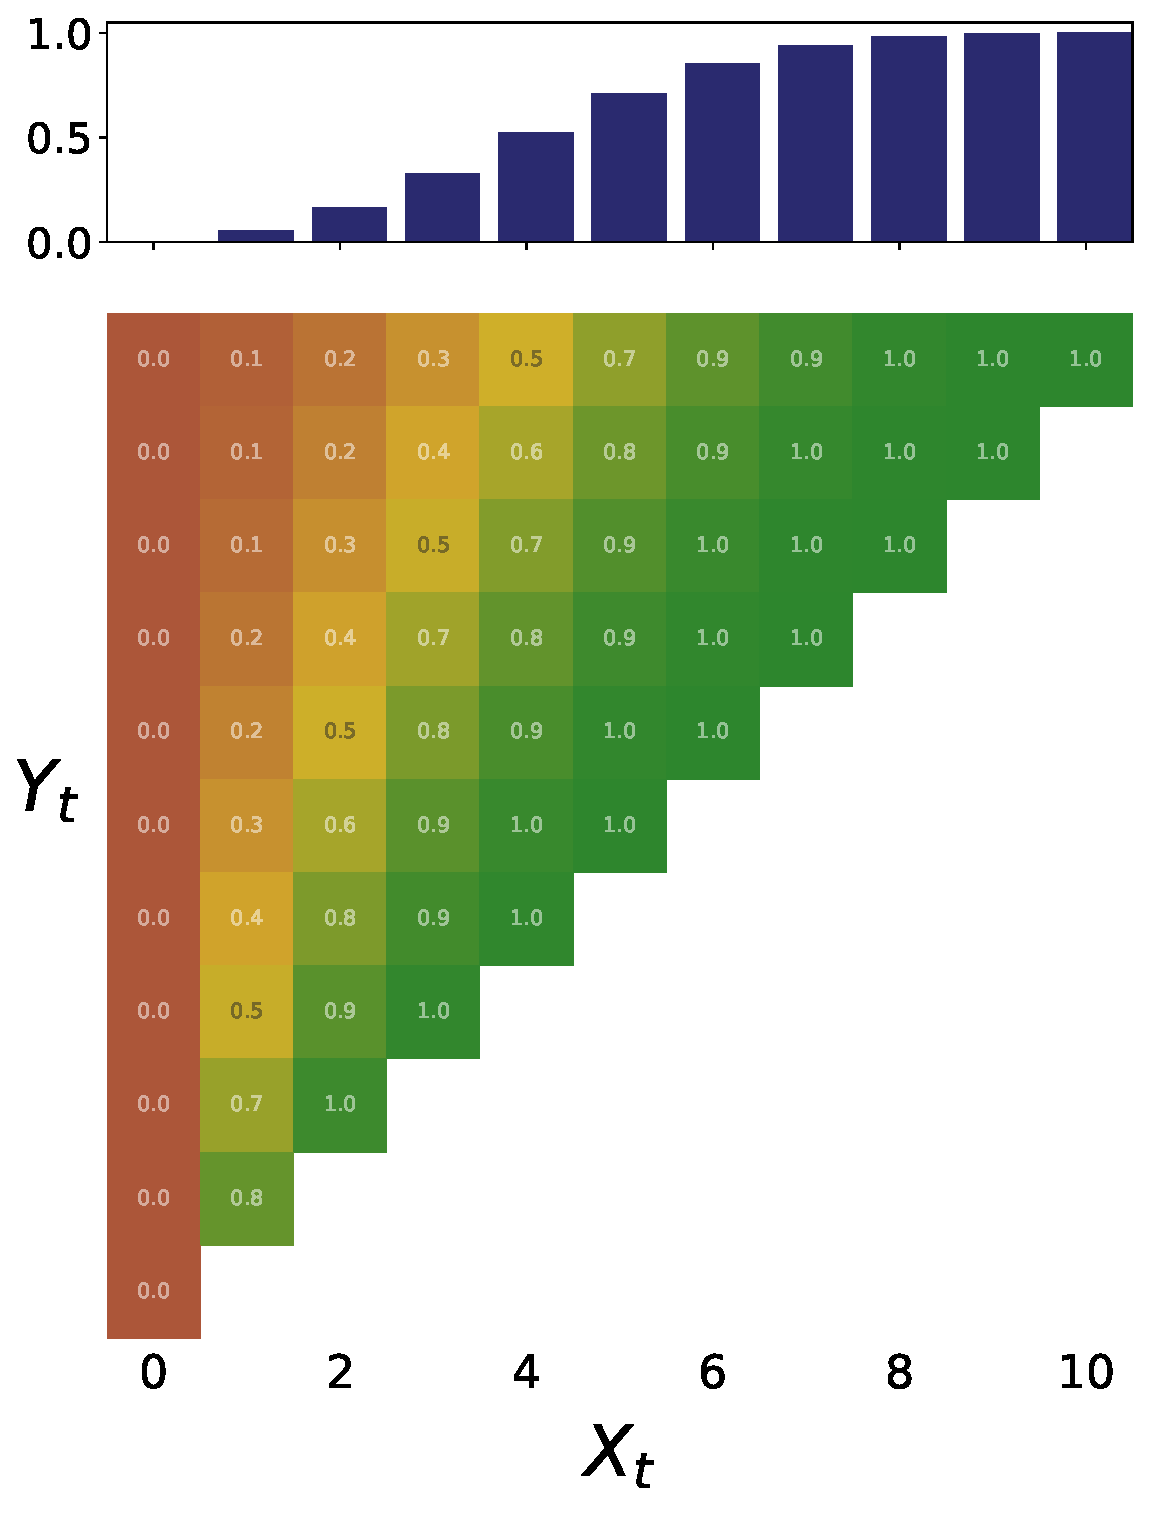
\includegraphics[width=\textwidth]{chapter7/IMG_ch7/RepSupp_10_0.2_1_NBA_.pdf}
        \label{fig:graph2}
    \end{minipage}\hfill
    \begin{minipage}{0.3\textwidth}
        \centering
       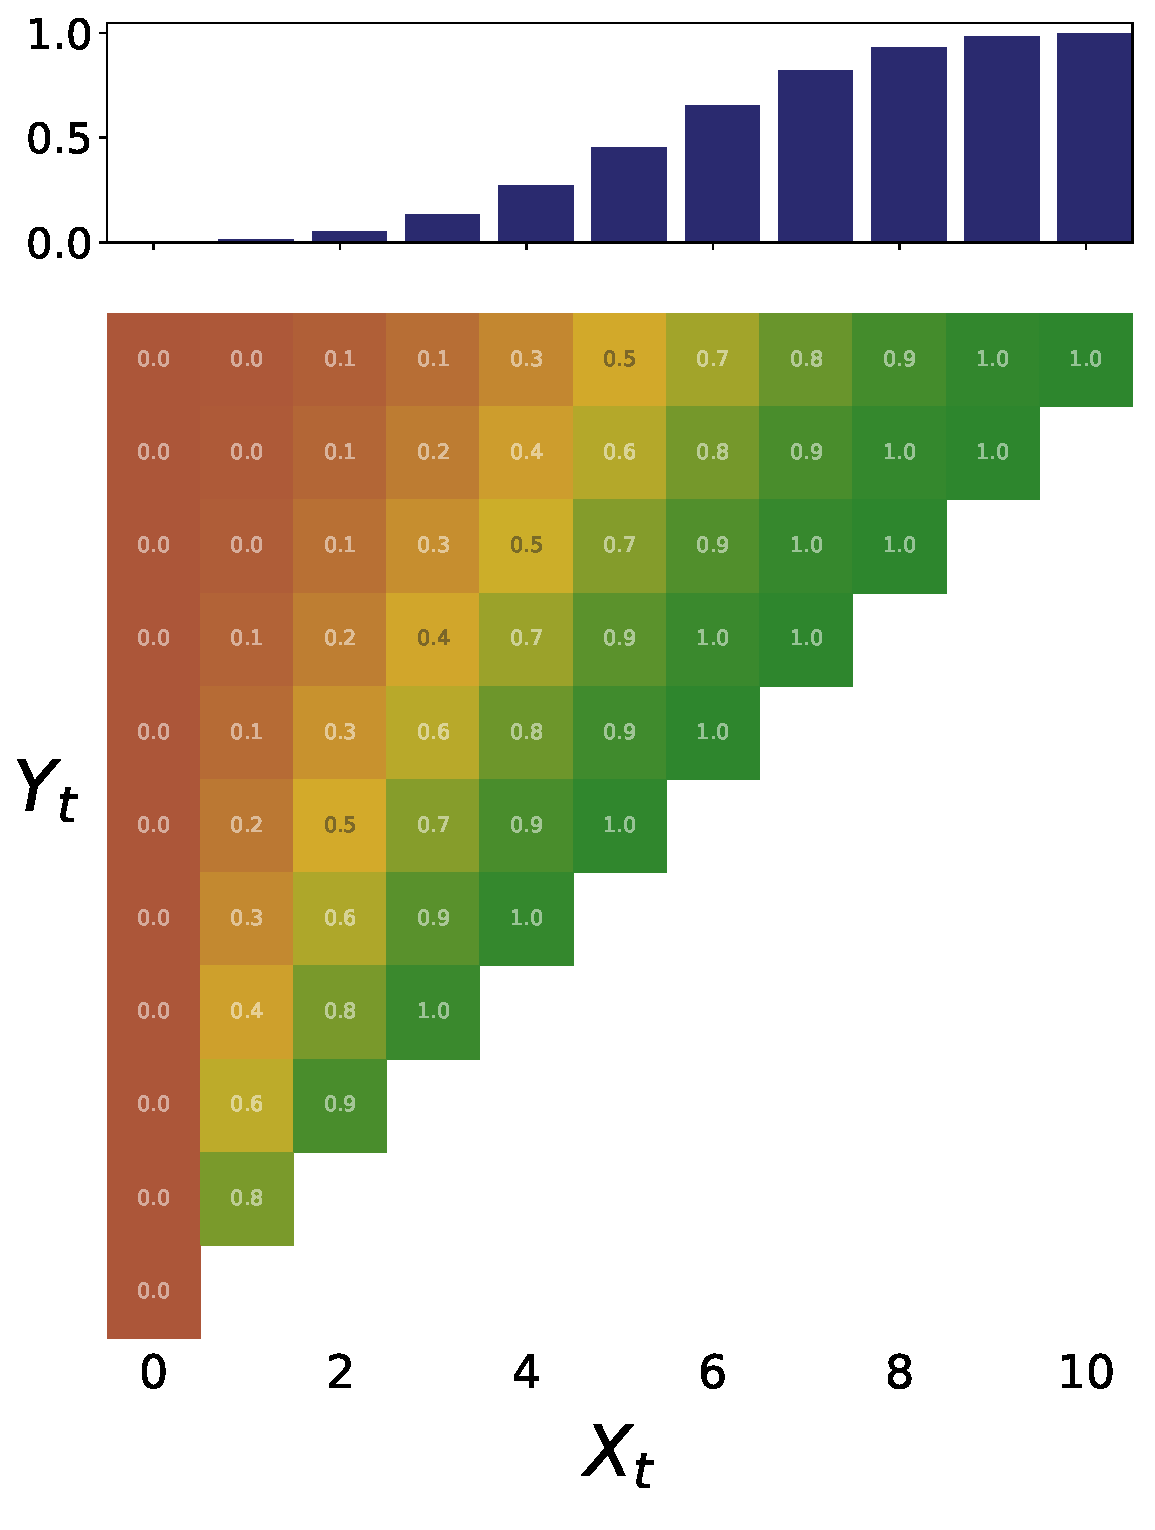
\includegraphics[width=\textwidth]{chapter7/IMG_ch7/RepSupp_10_0.3_1_NBA_.pdf}
        \label{fig:graph3}
    \end{minipage}
    \caption{For each count of immune granules, there is a critical requirement of incident pathogen for infection persistence to be likely.  This is all to demonstrate that immune granuls create a situation in which bursting dynamics with group transfer could be advantageous. The following section addresses the same sort of dynamics but with regards to extracellular immune factors.}
    \label{fig:threegraphs}
\end{figure}
















\begin{lstlisting}[language=Python]
import numpy as np 

N = 20
beta = 0.2
alpha = 1



def b_hat(i, j):
    return (beta * j) / (alpha + beta * j) 

def a_hat(i, j):
    return alpha / (alpha + beta * j)



def generate_Asub(i, j):
    '''produces the A sub-matricies'''
    dim1 = N + 1 - i
    dim2 = N + 1 - j
    Asub = np.zeros((dim1, dim2))
    
    if j - i == 0:
        for k in range(N - j):
            Asub[k+1][k] = b_hat(k+2, k+1+j)
            
        
    if i - j == 1:
        for k in range(N - j):
            Asub[k][k+1] = a_hat(k+1, k+1+j)

    return Asub

def concatA(Amatrix):
    '''combines the A sub-matrices into the full A matrix'''
    w = Amatrix[0].size
    
    # first row
    newA = Amatrix[0][0]
    for j in range(1, w):
        newA = np.append(newA, Amatrix[0][j], axis=1)
    
    # other rows
    for i in range(1,w):
        segmentA = Amatrix[i][0]
        for j in range(1, w):
            segmentA = np.append(segmentA, Amatrix[i][j], axis=1)
        newA = np.append(newA, segmentA, axis=0)
        
    return(newA)

def full_A():
    '''uses above two functions to produce full A matrix'''
    Amat = np.zeros((N, N), dtype=object)
    for i in range(1, N+1):
        for j in range(1, N+1):
            Asub = generate_Asub(i, j)
            Amat[i-1][j-1] = Asub
         
    A_full = concatA(Amat)
    return(A_full)



def generate_Csub(i):
    '''produces the C sub-vectors'''
    dim = N + 1 - i
    Csub = np.zeros(dim)
    Csub[0] = b_hat(1,i)

    return Csub

def concatC(Cvector):
    '''combines the C sub-vectors into the full C vector'''
    newC = Cvector[0]
    for i in range(1, Cvector.size):
        newC = np.append(newC, Cvector[i], axis=0)
    
    return(newC)

def full_C():
    '''uses above two functions to produce full C vector'''
    Cvec = np.zeros(N, dtype = object)
    
    for i in range(1, N+1):
        Csub = generate_Csub(i)
        Cvec[i-1] = Csub 
    
    C_full = concatC(Cvec)
    
    return(C_full[:, np.newaxis])



def get2D_dist(theta_vector):
    '''converts the 1D array with the theta values into its 2D grid form'''
    out = np.zeros((N+1, N+1))
    
    out[0] = np.array([1]*(N+1))
    
    
    idx = 0
    for c in range(N):
        for r in range(N-c):
            i = r+1
            j = r+1+c
        
            out[i][N-j] = round(theta_vector[idx][0], 3)
            
            idx += 1
            
    return out.T



A = full_A()
C = full_C()



# prepares A matrix for linalg solve function 
Amod = np.identity(A.shape[0])-A

# gets theta vector solution 
solution = np.linalg.solve(Amod,C)

# converts to 2D form
dist_2D = get2D_dist(solution)

# switches result from \xt death to survival probability 
dist_2D_survival = np.ones((N+1, N+1)) - dist_2D

# extracts values relevant to initial conditions
ICvec = dist_2D_survival[0]
\end{lstlisting}














































%%%%%%%%%%%%%%%%%%%%%%%%%%%%%%%%%%%%%%%%%%%%%%%%%%%%%%%%%%%%%%%%%%%%%%%%%%%%%%%%%%%%%%%%%%%%%%%%%%%%%%%%%%%5


\section{Fixed removal}



In the pursuit of modelling multi-stage intracellular infection, we have been working on an iterated birth death catastrophe process with the assumption of complete transfer (chained ruptures). In trying to determine whether there is a fundamental reason for bursting dynamics in pathogenesis, this model is of limited efficacy. With agents replicating identically whenever they are within a host cell, it matters not how they are moved, just that they are replicating. With chained ruptures, the burst event is merely a recorded instance without tangible implication to agent spread. And if instead, the bacteria modelled were to make their way one by one to a new host, or even to multiple hosts, no change would be made to the expected growth rate of the overall population. Even if some delay were introduced for unit transfer between hosts, this would merely have the effect of adding intervals of inactivity to the time axis; broad propagation dynamics would remain identical.\par

It seems that if we wish to begin understanding why, or if there is a reason why, pathogens follow a bursting regime of infection, we must consider additional factors. Namely, we must take into account that the death and replication rates of individual agents are not entirely independent to the surrounding cohort. For example, various of the bodies immuno-factors are depletable. For instance, leucocytes including macrophages and neutrophils contain on the order of 10 so called granules. Small packets containing oxidising compounds with a toxic effect on invading pathogens. Given these can be used up, the effective within-host death rate of infectious agent will reduce as more and more of the incident cohort are killed. There are likely extracellular immune factors which exhibit a similar pattern of depletion.\par

Here is presented an extension to the ``chained rupture'' model. There is included a simple assumption which arises from an argument of immuno-depletion: that following a burst release event, some defined fixed count of the agents are removed. This is used as the basis for attempting to understand whether bursting pathogenesis strategies might be of fundamental advantage in relevant cases.


\subsection{Successive birth death catastrophe}
\noindent
The concept of chained ruptures is simple. A series of BDC processes follow on from one another, the result of the last going on to found an initial condition for the next.\par
Starting with an single replicative unit, the first process undergoes the standard dynamics of birth and death. Then, at the time of the catastrophe event, the quantity of units present is, as it were, immediately transfers into another target cell founding the second process with its initial condition as given. This is the main assumption: that released replicative units somehow find their way, all at once, to the same host cell. Of course this is quite reduced from the biological context.\par
A less restricted view would be that following rupture, all of the $r_1$ released bacteria undergo Brownian motion and drift gradually from the burst location. The cohort, as it spreads out will encounter multiple new target cells and get taken up one by one. Albeit less so, this is also greatly reduced from biological reality, which in its full complexity will be beyond the scope of concise mathematical description. For example, the target cells we have focused on mostly are macrophages. Macrophages do not merely float around in Brownian drift; they are motile, and essentially walk around their environment seeking out debris and alien material to engulf and make away with. The agents themselves are little more straightforward. Yersinia pestis can ``decide'' whether it will be absorbed or not by such phagocytes. In addition to this, the bacteria can inject immune cells with a host of special proteins with various effects including neutralisation.\par
Generally, the playing field of these actors is just that, an environment of play, in which the responsive agents interact with one another; causal relationships ensue which go far beyond mere drift and chance.\par

\subsection{Extracellular removal}






\begin{figure}[H]
    \centering
    % First figure
    \begin{subfigure}{0.31\textwidth}
        \centering
        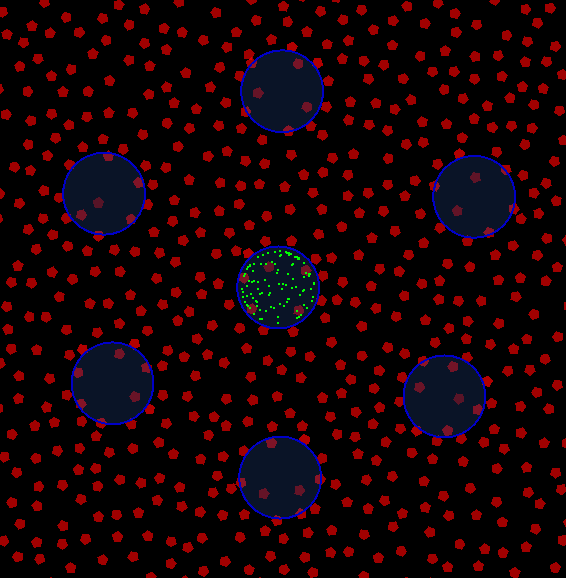
\includegraphics[width=\textwidth]{chapter7/IMG_ch7/Bursting/FR/big1} % Adjust the image path as necessary

        \label{fig:figure1}
    \end{subfigure}
    \hspace{\fill} % Optional: adds space between figures
    % Second figure
    \begin{subfigure}{0.31\textwidth}
        \centering
        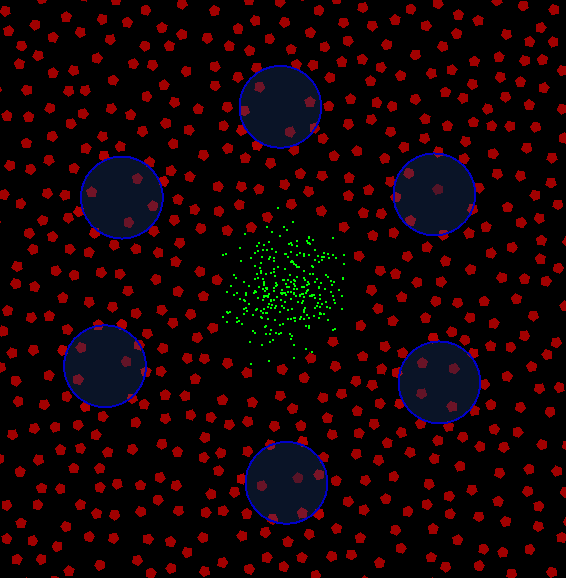
\includegraphics[width=\textwidth]{chapter7/IMG_ch7/Bursting/FR/big2} % Adjust the image path as necessary
    
        \label{fig:figure2}
    \end{subfigure}
    \hspace{\fill} % Optional: adds space between figures
    % Third figure
    \begin{subfigure}{0.31\textwidth}
        \centering
        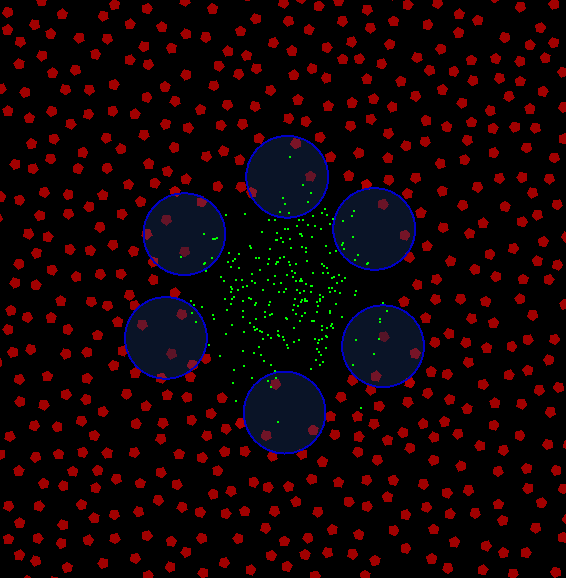
\includegraphics[width=\textwidth]{chapter7/IMG_ch7/Bursting/FR/big3} % Adjust the image path as necessary
    
        \label{fig:figure3}
    \end{subfigure}

    \caption{In the above simlation run snapshots, it is demonstrated that given the presence of depletable extracellular immuno factors, a larger released pathogenic load creates a safety in numbers "flooding effect" leading to more incident pathogen in surrounding host cells.}
    \label{fig:three_figures}
\end{figure}






\begin{figure}[H]
    \centering
    % First figure
    \begin{subfigure}{0.31\textwidth}
        \centering
        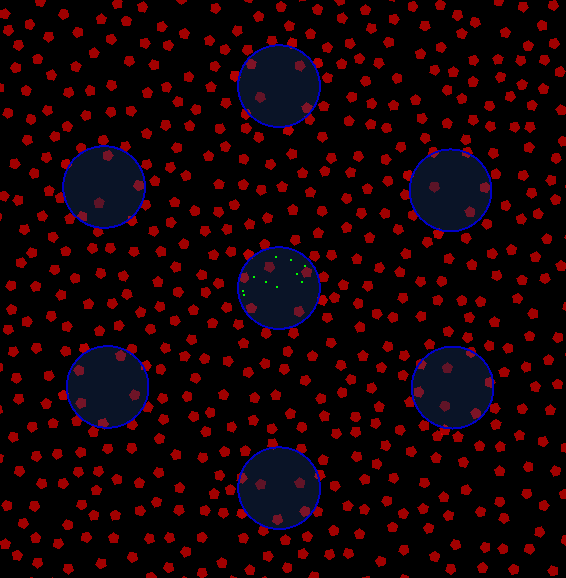
\includegraphics[width=\textwidth]{chapter7/IMG_ch7/Bursting/FR/small1} % Adjust the image path as necessary
        \label{fig:figure1}
    \end{subfigure}
    \hspace{\fill} % Optional: adds space between figures
    % Second figure
    \begin{subfigure}{0.31\textwidth}
        \centering
        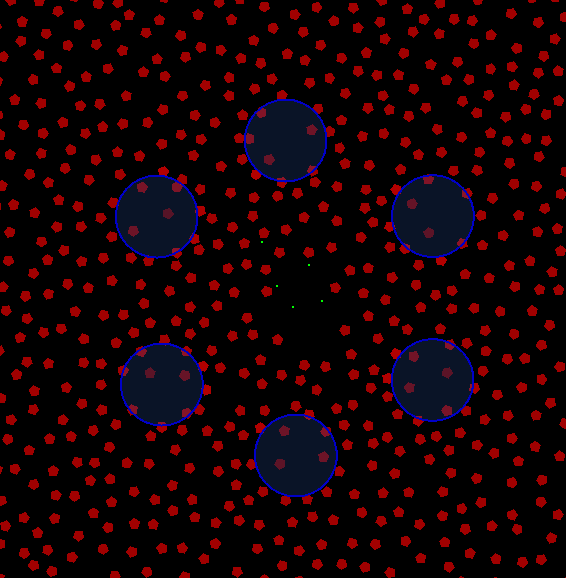
\includegraphics[width=\textwidth]{chapter7/IMG_ch7/Bursting/FR/small2} % Adjust the image path as necessary
        \label{fig:figure2}
    \end{subfigure}
    \hspace{\fill} % Optional: adds space between figures
    % Third figure
    \begin{subfigure}{0.31\textwidth}
        \centering
        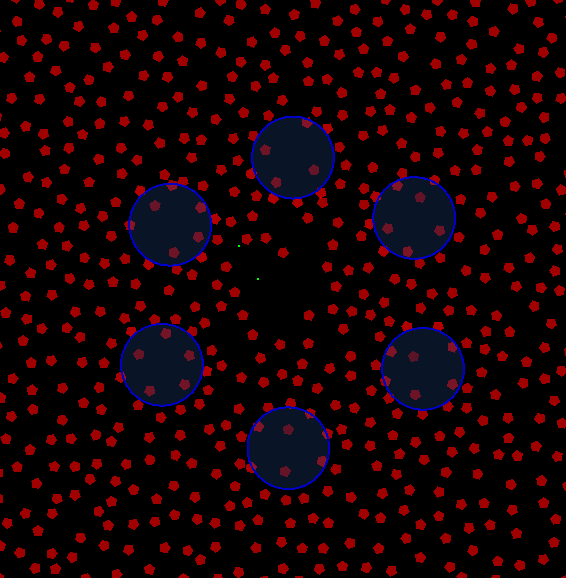
\includegraphics[width=\textwidth]{chapter7/IMG_ch7/Bursting/FR/small3} % Adjust the image path as necessary
        \label{fig:figure3}
    \end{subfigure}

    \caption{Contrasting the above situation, a small released load may be depleted without persistence to the next rounds of intracellular absorption and replication.}
    \label{fig:three_figures}
\end{figure}




\subsubsection{The assumption}
But let us humour it --- this concept of spatial drift. Despite imperfection, it does improve on the simpler dynamic of chained immediate transfer. Picture the playing field: a three dimensional extracellular matrix populated by three types of agents: replicative units (pathogen), Host cells (Macrophages), and another type of immuno-active cell; we'll call them simply ``killer cells''. This third type is able to eliminate the units of pathogen on contact, being used up in the process; one to one encounters where a killer cell removes a replicative agent and itself from play.\par
To begin with, the extracellular matrix is populated evenly with target cells and killer cells, each group occupying the space in a uniform spatial density. Killer cells are smaller and more numerous than target cells; a greater number per unit volume. Dynamics within target cells are as we understand in the birth death catastrophe process. The units of pathogen replicate and die within the cell until eventually rupture is caused and the load is released.
In this model, we are considering movement to be Brownian. An extracellular colony will drift from their burst location, spreading out and coming into contact with surrounding cells. Some will encounter target cells, others, killer cells. Now... my intention with this is not to construct a full mathematical description of this model game. This would be cumbersome and intractable. It will be possible to simulate it computationally, and this may prove helpful in supporting the assumption which I hope to use the model to justify. If we suppose that no new killer cells are introduced into the environment. An assumption that pathogen movement and absorption occurs on a shorter time scale thank killer generation. Then, with greater burst sizes, each individual bacteria will have a smaller probability of being removed. Those at the leading edge, as it were, clearing the way for their comrades in the rear.

If it happens that free agents do tend to find a new host before long --- an assumption taken to the limit in the case of chained immediate transfer --- this above observation offers the basis of an approximate mathematical rule. That is, there will be a relationship between burst size and the number of pathogen killed in the process of transfer. 

As bursts of greater and greater number are compared, the casualty count will increase more and more slowly. Qualitatively this might be like a logarithmic progression.

$$\theta(r) \sim \log(r+1),$$  
where $r$ is a given burst size and $\theta$ is the number of replicative agents removed by killer cells. (The +1 is simply to make the curve go through the origin).



\begin{figure}[H]
\begin{center}

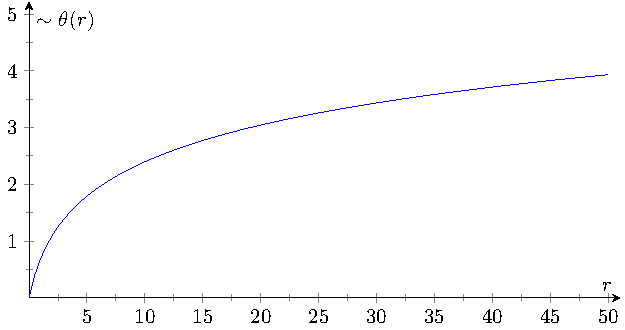
\includegraphics[width = 0.7\textwidth]{chapter7/IMG_ch7/log_plot1.pdf}

\end{center}
\caption{Qualitative representation of the deminishing removed count $\theta(r)$, given released numbers.}
\end{figure}
    

\noindent
Given this to be the case, it might prove reasonable to impose a fixed removal following release. In this construction, the number removed by killer cells will be a specified constant, regardless of burst size. Though, if the burst size is less than this constant, simply all of the units will be killed. 
$$\text{removal} = \begin{cases}
& r , \quad \text{ if }r \leq \theta\\
& \theta, \quad \text{ if } r>\theta.
\end{cases}$$
Now taking $\theta$ to be a constant.

	
\begin{figure}[H]
\begin{center}

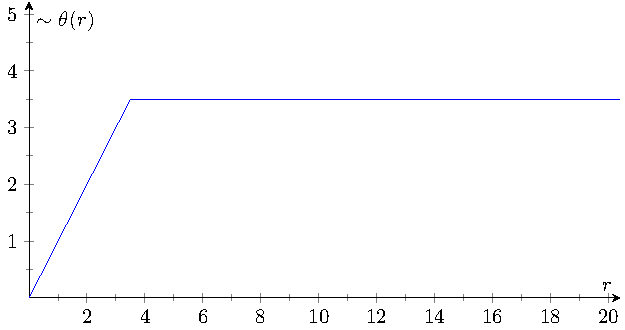
\includegraphics[width = 0.7\textwidth]{chapter7/IMG_ch7/log_plot_square.pdf}

\end{center}
\caption{An approximate representation of the above shown (figure above) diminishing removel effect.  Fixed removal count $\theta$ facilitates analysis of proliferation number.  (the number of new infections provided by a single burst event assuming one pathogen per new host.)}
\end{figure}

    
    
    


\noindent
The potential efficacy of this assumption rests in the likelihood that the same qualitative dynamics will be shared with the case of logarithmic removal (or whatever the actual relation is, assuming it is of this sort). 

There are a couple of points to address.
\begin{itemize}
\item I want to impose a further assumption: that at the time of each rupture event, the killer cell prevalence has returned to it's steady state and is once again of uniform spatial distribution.

\item We may frame the ``fixed removal'' dynamic in the context of chained transfers where all agents released have the same target cell to go to. Or, we may consider a case in which each successful pathogenic unit goes on to found an infection in a new target cell. 
\end{itemize}

\vspace{10pt}


\hrule
\vspace{5pt}

\noindent
\textbf{Aside:} In the case where all surviving agents go directly to the same host cell, we can potentially frame the replication ratio as follows: Expected number of surviving released units \textit{per incident agent}. 
\hrule
\vspace{8pt}


\vspace{10pt}


\noindent
Let us for now take this second option --- that each released cell goes on to found a new infection in a new target cell. We can consider the effective replication number between target cell infections. That is, the expected number of newly infected target cells created by a given host of one initial bacterium. Because each surviving released infectious particle infects a new host, the replication number is simply the expected quantity of these survivors. 

\subsubsection{Intra-burst replication ratio}
To begin with, we must define $r$: the outcome of a BDC process with a single incident unit. Mainly, we much choose, whether or not to include outcomes that are 0 due to process death. It makes practical sense for our purpose to choose this option, to not ignore cases of $r = 0$. With this $\mean{r} = \lim_{t\to\infty} \mean{\yt} = V_{\text{inf}}$.\par

The number that survive our fixed removal will be $\max({0, r-\theta})$. Hence, the expected replication number is
$$R_0 = \mean{\max(r-\theta, 0)}.$$
We can deconstruct this based on whether the burst size is bigger or smaller than $\theta$:
\begin{align*}
\mean{\max(0, r-\theta)}  &= \mean{r-\theta | r \geq \theta} \pr{r\geq \theta} + \cancelto{0}{ \mean{0}\pr{r<\theta}}\\
& = \lrbs{\mean{r| r\geq \theta} - \theta}\pr{r\geq\theta}
\end{align*}
Then, we can extract $\mean{r|r\geq\theta}$ in the following way. 
$$\mean{r} = V_{\text{inf}}= \mean{r|r\geq\theta}\pr{r\geq 0 }  + \mean{r | r < \theta }\pr{r < \theta}$$
With 
$$\pr{r<\theta} = \sum^{\theta - 1}_{i=0} \pr{r = i},$$
$$\pr{r\geq \theta} = 1- \pr{r<\theta} ,$$
and,
$$\mean{r|r<\theta} = \sum^{\theta - 1}_{i=1} i \pr{r = i| r < \theta} =  \sum^{\theta - 1}_{i=1} i \frac{\pr{r = i}}{\pr{r < \theta}},$$
we can make the rearrangement,
\begin{align*}
\mean{r|r\geq\theta} &= \frac{\mean{r} - \mean{r|r<\theta} \pr{r<\theta} }{\pr{r\geq \theta} }\\
&= \frac{\mean{r} -       \sum^{\theta - 1}_{i=1} i \frac{\pr{r = i}}{\cancel{\pr{r < \theta}}}  \cancel{\pr{r<\theta}} }{\pr{r\geq \theta} }\\
&= \frac{\mean{r}  -   \sum^{\theta - 1}_{i=1} i \pr{r = i} }{1 -  \sum^{\theta - 1}_{i=0} \pr{r = i}}.
\end{align*}
This is analytically computable because we have 
$$\pr{r=i} = \frac{\delta}{\lambda}\lrb{\frac{1}{a}}^i$$
$$\mean{r} = V_{\text{inf}}. $$
Hence,
$$\mean{\max(0,r-\theta)}  =  \lrbs{  \frac{\mean{r}  -   \sum^{\theta - 1}_{i=1} i \pr{r = i}}{1 -  \sum^{\theta - 1}_{i=0} \pr{r = i}}   - \theta} \pr{r\geq \theta}  $$
becoming 
$$\mean{\max(0,r-\theta)}  =  \lrbs{ \frac{V_{\text{inf}} -  \mathcal{K} }{1 -  \mathcal{G}} - \theta} \lrb{1 - \mathcal{G}}  = V_{\text{inf} }-  \mathcal{K} - \theta ( 1 -  \mathcal{G})$$
where 
$$\mathcal{G} = b+ \sum^{\theta - 1}_{i=1} \frac{\delta}{\lambda}\lrb{\frac{1}{a}}^i   \quad\text{ and } \quad \mathcal{K} =  \sum^{\theta - 1}_{i=1} i  \frac{\delta}{\lambda}\lrb{\frac{1}{a}}^i . $$
Because the formula 
$$\pr{r=i} =  \frac{\delta}{\lambda}\lrb{\frac{1}{a}}^i$$ does not correctly apply when $i = 0$, this is why the sum for $\mathcal{G}$ begins at 1, and why there is the term, $b$, preceding the sum. This is the probability that the process ultimately ends in death, an output of 0. 


\vspace{10pt}
\noindent
\textbf{Direction.} The primary interest is in whether this value is greater or less than 1, and if greater, by how much. And the question is in how this changes with $\delta$. Do larger burst sizes make an infection more viable and proliferative?\par
Before proceeding with this analysis, we should verify whether the formula is correct using numerical simulation comparisons.    

\subsubsection{Verification of formula}
Compare replication ratio from formula with equivalent numerical results from simulations ...

We must be clear as to whether $r$ includes bust cases alone, or whether it factors in cases of death. Bear in mind that the formula for $\pr{r = i}$ is not defined when $i=0$, in this case, $\pr{r = 0} = I_-$.\par
An observation: The formula for $\pr{r=i}$, does not apply to $i=0$. We know the probability that $r=0$. It's $I_-$, or $b$, or $\eta^2 + \sqrt{\eta^2-\mu/\lambda}$. Furthermore, it can be shown that 
$$I_- + \sum_{i=1}^{\infty} \pr{r=i } = 1:$$
$$ \sum_{i=1}^{\infty}\frac{\delta}{\lambda}\lrb{\frac{1}{a}}^i = 1 - b. $$
Then using the geometric sum formula $\sum_{k=1}^{\infty} y^k = y/(1-y) $ ($|{y}|<1$),
$$\frac{\delta}{\lambda} \lrb{\frac{\frac{1}{a}}{1 - \frac{1}{a}}} = 1 - b$$
$$\frac{\delta}{\lambda} = (1-b)(a-1) = (a+b) - ab - 1$$
With $a+b = \frac{\lambda + \mu + \delta}{\lambda}$ and $ab = \frac{\mu}{\lambda}$, it can be shown that the LHS does equal the RHS,
$$\frac{\delta}{\lambda}  =  \frac{\lambda + \mu + \delta}{\lambda}  -  \frac{\mu}{\lambda} - 1 = \frac{\delta}{\lambda} $$. 
This is all to say that we can be quite certain of the fact that 
$$\mathcal{G} = \pr{r < \theta} = I_- + \sum^{\theta - 1}_{i = 0} \frac{\delta}{\lambda}\lrb{\frac{1}{a}}^i$$


\subsubsection{Analysis of proliferability} 
Basically, how does the replication ratio change depending on the burst rate (burst size) ...

To begin with, we can take the formula found,
$$\mean{\max(0,r-\theta)}  = V_{\text{inf} }-  \mathcal{K} - \theta ( 1 -  \mathcal{G}),$$
and make it easier to analyse. Because $|\frac{1}{a}| < 1$, we can use the following geometric sum identities to re-write $\mathcal{G}$ and $\mathcal{K}$.
$$\sum_{i=1}^{n-1} = \frac{s\lrb{1-s^{n-1} }}{1-s} $$
$$\sum_{i=1}^{n-1} = \frac{s\lrb{1 - n s^{n-1}  +(n-1) s^{n}  } }{ (1-s)^2}. $$

\noindent
With, $s = \frac{1}{a} $ and $n = \theta$, it can be shown that $\mean{\max(0,r-\theta)}  $ becomes
$$\mean{\max(0,r-\theta)}  = V_{\infty} - \theta(1-b) + \frac{\delta}{\lambda} \lrb{     \frac{\frac{1}{a}\lrb{ \theta - 1 - \theta \frac{1}{a}  +\lrb{\frac{1}{a}}^\theta  }      }{\lrb{1 - \frac{1}{a}}^2}  } $$







\begin{figure}[H]
    \centering
    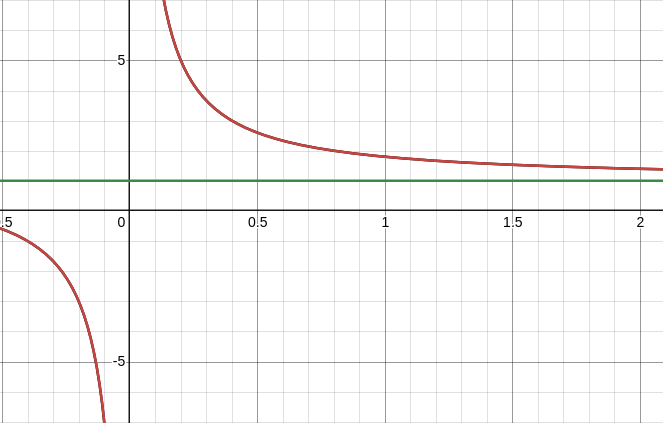
\includegraphics[width=0.7\textwidth]{chapter7/IMG_ch7/FR/FRH0} % Adjust the width as needed
    \caption{$\lambda$ = 0.8 $\theta$ = 0.  x-axis: $\delta$. With smaller delta, there is an increasingly large burst size.  In this plot the removal value, $\theta$ is 0. On the y-axis is the quantity $ \mean{\text{max}(0, r-\theta)} $  and $\mean{r}$, the mean release without removal. When $\theta = 0$, these two values are obviously the same, and the lines overlap. In the figures below,  $\theta  \neq 0$,  and the lines do not overlap.}
    \label{fig:sinfigure}
\end{figure}



\begin{figure}[H]
    \centering
    % First figure
    \begin{subfigure}{0.48\textwidth}
        \centering
        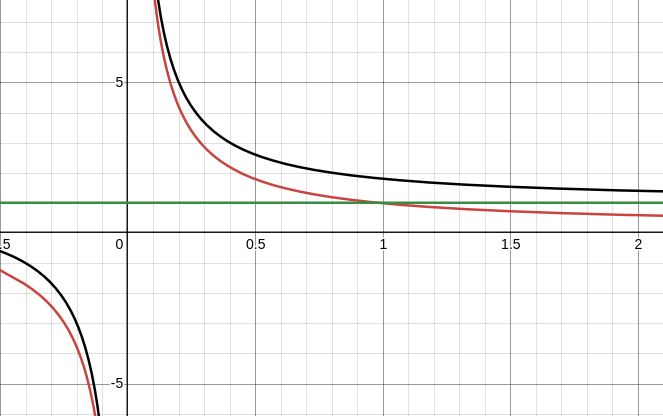
\includegraphics[width=\textwidth]{chapter7/IMG_ch7/FR/FRH0p8} % Adjust the image path as necessary
    \end{subfigure}
    \hspace{\fill} % Optional: adds space between figures
    % Second figure
    \begin{subfigure}{0.48\textwidth}
        \centering
        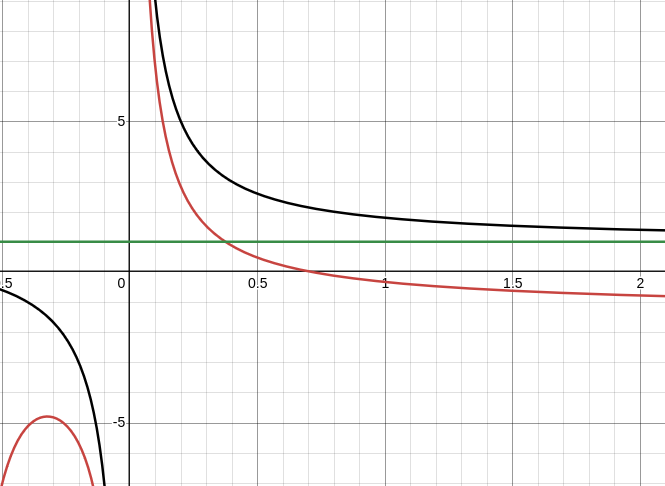
\includegraphics[width=\textwidth]{chapter7/IMG_ch7/FR/FRH2p3_L0p8} % Adjust the image path as necessary
    \end{subfigure}
    
    \caption{It can be seen that when $\theta > 0$, the required $\delta$ to ensure supercritical proliferation ($\mean{\text{max}(0, r-\theta)} > 1$) is smaller (the required release size is higher). ( $\lambda$ = 0.8, $\theta$ = 0.8 and $\theta = 2.3$ (left and right respectively))}
    \label{}
\end{figure}



















\subsubsection{Motivation}

I am interested in the question of whether there is some fundamental advantage to bursting dynamics in pathogenesis. In the case of \ft \, and \yp, hot cell lysis may be caused merely as the simplest means of release. With bacteria being relatively large in comparison to the protein complexes that constitute a cell membrane, it would be difficult to employ a strategy in which some but not all of the pathogen are released. The case of viruses is different. They are sufficiently small to allow for partial release of an intracellular load. To be fair, in the case of viruses such as HIV, there is an explicit advantage to not killing the cell: its machinery continues to produce virions. Despite this, I have a suspicion that there is some advantage to bursting style strategies. That is, where agents are released in large groups all at once from their hidden position within host cells. As opposed to continually, or in dribs and drabs. There are a great many stories one could tell about the reason for which this might be the case, that there is an advantage to bursting. Here are three categories in which the ones I've thought up fall under. 

\begin{itemize}
\item \textbf{Subductive proliferation.} Replication rate reduces over time within a host cell, perhaps following recognition, or by the using up of available resources. (Though to be honest, I'm starting to think that this doesn't check out as a reason --- some analysis should reveal the truth one way or the other).
\item  \textbf{Limited extracellular killing.} As described above, the means of removing agents are finite on relevant timescales, this leading to an effective reduction in death rate for invading pathogen. Note: this dynamic my take place either inside the cell or extracellularly as described above. For the case of within cell dynamics, some host cells contain oxidative granules, which in their finite number, destroy intracellular agents.  
\item \textbf{Detection avoidance}
For the case of HIV, where observations have been made that release is sporadic and clustered. There may be some argument against a strategy of continual budding because it might lead to more effective detection by targeting immune cells which induce apoptosis. 
\end{itemize}
Each argument of these three types essentially boils down to the catching off guard of some immune mechanism. As it were, surprising the systems of regulation to the extent that response is too slow. 






\subsubsection{Potential for \yp}

We might be able to frame this model in the context of Y. pestis and neutrophils. That is, the target cells are macrophages, the killer cells are neutrophils. And the reason for the two phases of infection is argued for by firstly, the advantage of bursting in the case of constant density killer cells, then secondly, the mass increase in killer cells causes a need to become extracellular. But this would beg the question: why not just replicate extracellularly from the beginning. There must be some advantage to being within macrophages. For one thing, they are a means of transport. Taking the agents to lymph nodes where there is lots of food. They may provide food themselves.  




\section{Note about quad tree sampling}

To speed up the animations, I ported an open-source implementation of quadtree sampling from JavaScript to C++. It works by sorting all of the particles into a structured index (characterized by hierarchical branching of squares within squares). When checking if one of the particles intersects with the macrophage's circle, only those local to the macrophage are checked. Locality is determined and identified by the position in the quadtree. Below, there is a figure in which the local regions of the macrophage are shown in pink. Only the green dots in those squares are checked for collisions. The entire tree index needs to be recreated every frame, but despite this, the speed increase is worth it, especially in the case shown in the image on the right.




\begin{figure}[H]
    \centering
    % First row of two figures
    \begin{subfigure}{0.48\textwidth}
        \centering
        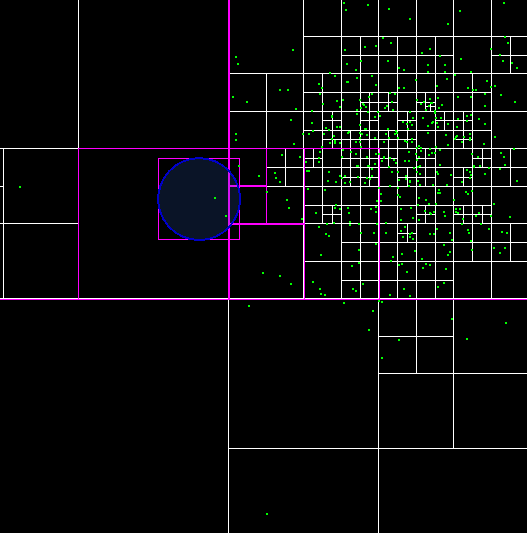
\includegraphics[width=\textwidth]{chapter7/IMG_ch7/Bursting/QTs/QT1} % Adjust the image path as necessary

        \label{fig:figure1}
    \end{subfigure}
    \hspace{\fill} % Optional: adds space between figures
    \begin{subfigure}{0.48\textwidth}
        \centering
        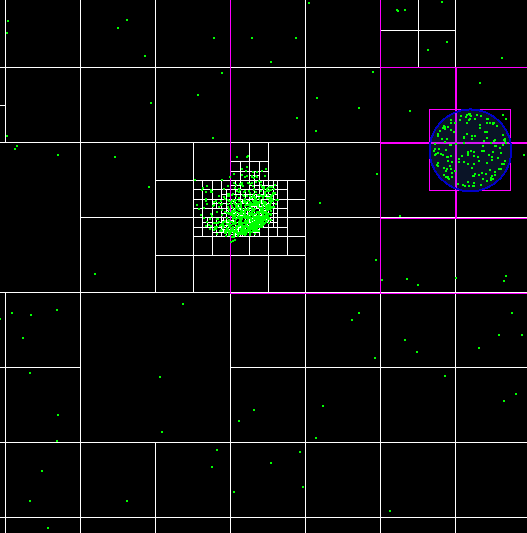
\includegraphics[width=\textwidth]{chapter7/IMG_ch7/Bursting/QTs/QT2} % Adjust the image path as necessary
      
        \label{fig:figure2}
    \end{subfigure}


    \caption{Visualization of the quadtree sampling used in the particle simulations shown above. Please refer to Wikipedia for more information on this; it's quite a well-worn topic in computer graphics.}
    \label{fig:four_figures}
\end{figure}







\chapter{Variability in evolution}











\subsection*{Speculative apocrypha}



When a group has dominion over an excess supply of resources, its selective pressures will be lessened by ease of replication without struggle, less offspring persisting and passing on variation.

This causes the ever-present potential for variability to become manifest, resulting in a smooth spectrum of divergences and variations. 

As the population expands to meet the supply of resources, the selective pressures begin to return, and what has become a sprawling range of variants once more becomes subject to the formative influence of selection. This begins to ``lock in'' an array of increasingly distinct sub types as the convergence to local optima commences. 

As species begin to move at odds with one-another, there begins competition for the once shared domain. Competitive exclusion may drive types into various distinct sub-niches. But where there is direct overlap, the Matthew effect takes hold, with those species that have some advantage benefiting secondarily from an increase of dominance. 

In this way, what became a huge multiplicity of forms gets reduced. Only a few will persist beyond the day after tomorrow. Only those with some edge, or that were able to secure the early monopoly.

In this way, a substantial easing of selective pressures can cause a stepwise morphological change consistent with the paradim of punctuated equalibria. Much speculation could be made into the possable causes of such a change of conditions. 

The expansion of a genus into a un-exploighted region
Perhaps like the first insects on dry land with a multitude of mosses and small shrubs to feast on. 
Even the first vertebrates that learned how to eat insects. 

Those left after a mass extinction event
Like the small mammals who inherited great swaths of fertile forests after dinosaurs were wiped out at the KT boundary. 

There is speculation that the Cambrian explosion was triggered by some combination of a huge global ice age and a great surplus of oxegen

Speculation has also been made that the evolutionary scale transition from prokaryotes to eukaryotes took place at a time of great surplus oxygen. 

Going beyond the domain of organic life, emergence and divergence of viral models may have followed a similar trajectory. A great variety of models were trialed during a flurry of funding and research into HIV in the early 90s. Over time, only a hand full of these went on to become commonplace.  




Qualitatively, we see that something like this has happened at various times across differing domains. In the first few million years after the cambrian explosion, there were a great variaty of arthropodic forms. 24 classifications have been counted amongst the remains of the Burgess shale. Over time this number was reduced to four main structures: chelicerata (arachnids), crustacea (crustaceans), hexapoda (insects and springtails), and myriapoda (millipedes and centipedes). For about half of the time since then, there were also trilobites, but these eventually dies out. 



\begin{figure}[h!]
    \centering
    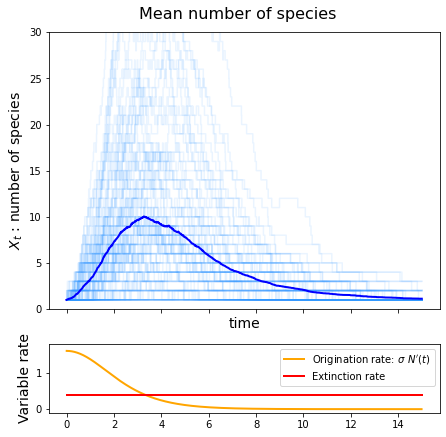
\includegraphics[width=0.7\textwidth]{chapter8/IMG_ch8/LSMean} % Adjust the width as needed
    \caption{Realisations of the logistic speciation model. Many realisations are shown in light blue. Their average is numerically calculated from these and shown in dark blue. It can clearly be seen that this model exhibits a period of heightened diversification when resources are relatively abundant before seeing a reduction as remaining capacity becomes scarce.  In real evolutionary processes, the latter stage of this procedure might be characterised by a smooth range of types diverging into a few distinct and optimised species which then compete and become subject to the Matthew effect.  Then, either a small number of the fixed types win out, or a number each find slightly different ecological niches to occupy.}
    \label{fig:single_figure}
\end{figure}



\section{Push of the past and Pull of the present}


With regards to the standard birth death process in which the condition of survival to the present is imposed (Quoting R.  Mann and G. Budd, who themselves were overviewing the topic introduced by Nee et.  al.):


\begin{quotation}
\noindent
"The POTPa emerges as a feature of diversification by the fact
that all modern clades (tautologically) survived until the present
day. This singles them out from the total population of clades
that could be generated from any particular pair of background
birth and death rates: clades that happened by chance to start off
with higher net rates of diversification have better-than-average
chances of surviving until the present day. As Nee et al. (1994a)
put it, such clades “got off to a flying start”; and they accumu-
late species faster than one would expect. Once clades become
established, they are less vulnerable to random changes in the
observed diversification rate, and this value therefore tends to re-
vert to the background rate through time. Long-lived clades thus
tend to show high observed rates of diversification at their origin,
which then decrease to their long-term average as the present is
approached."
\end{quotation}

\noindent
In their paper, "History is written by the victors," R. Mann and G. Budd propose that the push of the past (POTPa) is an underappreciated phenomenon in the paleontological literature, which delves into mass radiations following mass extinctions.
Without directly opposing their work, I present a model that illustrates a dynamic of variable-rate evolution, which also seeks to shed light on the higher origination rates of species following extinctions and events of ecological instability more generally \cite{bak1991self} \cite{fisher1929genetical}\cite{budd2018history}.







\section{Logistic speciation}







The number of individuals, or size of a population grows logistically according to standard logistic growth:
$$\ddt{N} = rN\lrb{1-\frac{N}{K}}.$$
The size of population, $N(t)$ is taken to be a continuous variable, a real number. It is assumed that this number of individuals is large compared to the count of species within the total group.\par

Types beget further variations in a descent of speciation that behaves as a Yule pure birth process. That is, given a number of types, $\yt$, initially 1, changes occur as defined: 
$$\pr{\yy_{t+\delt} - \yy_t = 1} = \beta \yy_t \delt + o(\delt)$$
taken in the limit, $\delt\to 0$. In the standard Yule process --- originally specified in 1924 to model the development of species --- $\beta$ is a constant value. Here however, we define this rate of speciation as a function of time. 
$$\beta \equiv \beta(t).$$
Such a step has been made before. Both in the field of evolutionary modeling, and elsewhere. If we were to set $\beta = \ee^{-t}$, the mean of $\yt$ would be described by the deterministic Gompertz model, introduced in 1825 \cite{gompertz1825xxiv}.\par

It doesn't appear that anyone has yet published a version of the model that uses the logistic function. There are a few ways of doing this, for now we will assign $\beta(t)$ the form, 
\begin{equation}
\label{rate1}
\beta(t) = \sigma\lrb{K - N(t)}.
\end{equation}
It serves as an index for the relative abundance of resources experienced by the population.\par

When $N(t)$ is small compared to the carrying capacity of the ecosystem, $K$, $\beta(t)$ is towards the higher end of it's range; species beget species with greather fecundity. We will later explore other options for the birth rate, for example, it may be sensible to ascribe the formula as $\beta(t) = \sigma\cdot \dd N/\dd t$ which would see the highest rate of division at the time of most rapid expansion --- perhaps this makes more sense than the fastest speciation beginng when the population is smallest. But for now let us continue with formula (\ref{rate1}). 

\vspace{10pt}
\hrule
\vspace{10pt}
\noindent
\begin{quotation}
\noindent
\textbf{Aside:} While writing this out, I am starting to wonder if the rate of population expansion is actually orders of magnitude faster than that of speciation. What if the logistic growth doesn't itself spur on type divisions, but instead lays out the potential for them. In this case, it would be incorrect to account for high early rates of speciation with the period of logistic expansion, however, such an expansion may mark the initial condition of a more DDD like model (density dependent diversification) such as the one we were initially working on.  \par

Could it be there is some effect whereby a homogeneos population experiences a saftey in numbers effect, i.e. a larger group has greater control of resorrces and its individuals are more protected from predators and competitors. In this case, the propensity to vary could be inflated. Then as the homogeneos group divides into ever smaller and smaller sub groups, they become more vulnerable --- this leading to harsher selection pressures and lower diversification rate.  
\end{quotation}
\vspace{10pt}
\hrule  
\vspace{10pt}

\noindent
The topic of variable variation in a group has been discussed by many thinkers: from Lamarck at the turn of the 19th centuary, to Darwin in the late 19th centuary; a number of more modern contributers such as S. J Gould in the latter 20th centuary. 
Somewhere in the middle, Ronald Fisher in his 1929 book, The Genetical Theorey of Natural Selection, implies that variations to a type are in constant and abundant supply, and that it is the harshness of environmental conditions in conjunction with sexual mixing which constantly work to quell this significant tendancy for genomes to become irretrievably disprate. 




According to Ronald Fisher, variations to the norm of a given type are in constant and abundant supply. It is the harshness of environmenal conditions which prevents many of them from becoming established; selection pressure supports adhearnce to a current optimal form. But when the selection pressures are lesser, when for example there are more comfortable conditions in the form of a fresh abundance of resources available to the population, variations to the norm are more likely to survive. 
\begin{quotation}
It is known by the experience of breeders that species which recieve superabundant nourishment, and in general a surplus of protection and care, immediately tend in the most marked way to develop variation, and are fertile in prodigies and monstrosities." (Nietzsche beyond good and evil section 262).
\end{quotation}

\begin{quotation}
"To maintain a stationary variance, fresh mutations must be available in each generation." (R. Fisher, the genetical theory of natural selection)
\end{quotation}

The whole thing is reminiscent of the concept described by Ilya Prigogine of dissipative structures. The idea being that where a flow of energy of matter is seen, structures can emerge which apparently go against the second law of thermodynamics. Locally, order can emerge as a spontaneous reduction in entropy. And this emergence is characterised by chaotic dynamics, its exact formation arising influenced by small fluctuations whos effects magnify and propergate.\par
Examples of dissipative structures can be seen throughout the natural world. It seems that one is the evolution of life into a multitude of forms and varieties.





\section{Model specification and results (no death case analytic soloutions)}

The following model is a version of the Yule process where the division rate, $\beta$, is a function of time. $\yt$ describes the number of species and it changes in continuous time according to the transition probabilities:


\begin{align}
\label{cases1}
\begin{split}
\pr{\yy_{t+\delt} - \pr{\yt} = 1} = \beta(t)\delt\yt + o(\delt)\\
\pr{\yy_{t+\delt} - \yt = 0} = 1 -  \beta(t)\delt\yt + o(\delt)
\end{split}
\end{align}
defined for $\delt\to 0$. \par
$N(t)$ is an index for the total population size, of individuals, constituting the sum of those in each $\yt$ species. Assuming the overall population is large, even from the beginning, $N(t)$ is defined as a real number. Starting at $N(0) = N_0$, the population develops acording to standard logistic growth: 
$$\ddt{N} = rN\lrb{1 - \frac{N}{K}};$$
Which permits description by the known formula, 
$$N(t) = \frac{K\ee^{rt}}{\xi + \ee^{rt}},$$
with the constant combination, $\xi = K/N_0 - 1$.\par
As discussed above, the model is set up to capture a variable speciation rate, and $\beta(t)$ varies with $N(t)$ to account for selection pressure --- higher when resources are less scarce. The exact form of $\beta(t)$ is a potential subject of experimentation. For now, we will  develop the case where
\begin{equation}
\label{basicRate1}
\beta(t) = \sigma\lrb{K-N(t)},
\end{equation}
but later, the following alternatives may also be explored:
\vspace{10pt}
\hrule
\vspace{10pt}
\noindent
\textbf{Alternative speciation rates}
\begin{itemize}
\item $\beta_2(t) = \sigma\lrb{K-N(t)} + \eta$,\\ ($\eta$ constant)
\item $\beta_3{t} = \sigma \ddt{N}$
\item $\beta_4{t} = \sigma \ddt{N} + \eta$
\item $\beta_5(t) = \sigma\lrb{K_t-N(t)}$,\\ with $K_t$ behaving according to some random switching regime (this may be a little too ambitions)
\end{itemize}
It may make sense for the speciation rate to depend on the rate of population increase rather than simply its size compared to availability of resource. With rapid individual replication, more opportunities are present for specific mutation events.\par
The incorporation of $\eta$ in case $\beta_2$ \& $\beta_4$ represents some baseline rate of variation, approached to at late time at the $N(t)$ reaches its steady state. This seems fitting to represent some underlying disequalibria in an ecosystem.  
\vspace{10pt}
\hrule
\vspace{10pt}

\noindent
With the above formula for $N(t)$, we can also write the division rate, (\ref{basicRate1}), as 
$$\beta(t) = \sigma\lrb{K - \frac{K\ee^{rt}}{\xi + \ee^{rt}}}$$
simplifying to 
$$\beta(t) = \sigma K \frac{\xi}{\xi + \ee^{rt}}$$


\subsection{Expectiation $\mean{\yt}$}
In the chosen case where $\beta(t)$ tends to 0 at late time, the final state of the process, $\yy_{t\to\infty}$, will arive at some fixed value. This could be thought of independently as a random variable with some mean, variance and distribution. Knowing more about this asymptoitc stationary distribution, we can ask questions surrounding how its nature depends on the parameters and their inyterplay. Here we will compute the mean, but we can do better than mearly compute its late time measure. It turns out quite straightforward to foumulate the expected value as a function of time; in this way we can see how the final position is approached. \par

If we consider how the expectation of $\yy_t$ changes over some vanishing interval, $\delt$, the mean after the interval is equivalent to the mean before plus the expected change;
\begin{equation}
\label{ExpectChange1} 
\mean{\yy_{t+\delt}} = \mean{\yt} + \mean{\yy_{t+\delt} - \yy_t}.
\end{equation}
And this latter term, the change, can be analysed in tems of the definition of the dirctete expectation, along with the possible cases and their associated probabilities (see (\ref{cases1})):

$$ \mean{\yy_{t+\delt} - \yy_t} = 0 \cdot \lrbs{1 -  \beta(t)\yt\delt} + 1\cdot \lrbs{\beta(t)\yt\delt} + o(\delt)$$
Ommitting the $\delt$, this simplifies to
$$ \mean{\yy_{t+\delt} - \yy_t} =  {\beta(t)\delt\yt} $$
which is equivalent to 
$$ \mean{\yy_{t+\delt} - \yy_t} =  {\beta(t)\delt\mean{\yt}}$$
(by taking the expected value of each side). Hence, with (\ref{ExpectChange1}), we can write
$$\frac{\mean{\yy_{t+\delt}} -  \mean{\yt}}{\delt} =    {\beta(t)\mean{\yt}},$$
or in the limit $\delt \to 0$,
$$\ddt{} \mean{\yy_t} = \beta(t) \mean{\yt}.$$
This is a seperable equation $\to$
$$\int\frac{1}{\mean{\yt}}\dd \mean{\yt}  = \int \beta(t) \dd t =  \sigma K \xi \int \frac{1}{\xi + \ee^{rt}} \dd t.$$
And with 
\begin{equation}
\label{intBetaT}
\int \frac{1}{\xi + \ee^{rt}} \dd t =\frac{1}{\xi} \lrb{ t - \frac{1}{r} \ln\lrb{\xi + \ee^{rt}} },
\end{equation}
it permits a solution in the following way.
$$\ln\lrb{\mean{\yt}} =  \sigma K\lrb{ t - \frac{1}{r} \ln\lrb{\xi + \ee^{rt}} }  + \text{const},$$
$$\mean{\yt} = C_0 \ee^{\sigma K\lrb{ t - \frac{1}{r} \ln\lrb{\xi + \ee^{rt}} } }.$$
The constant, $C_0$, is fixed with the initial condition, $\mean{\yy_0} = 1$:
$$C_0 = \ee^{\frac{\sigma K}{r} \ln\lrb{ \xi+1}}.$$
So
$$\mean{\yt} = \ee^{\sigma K \lrb{ t - \frac{1}{r} \ln\lrb{\xi + \ee^{rt}} +\frac{1}{r}\ln\lrb{\xi + 1} }}$$
and with some rearrangment, 
$$\mean{\yt} =  \ee^{\sigma K t} \lrb{\frac{\xi + 1}{\xi + \ee^{rt}}}^{\frac{\sigma K}{r}}.$$ 






\subsection{Probability generating function $G_{\yt}(z, t)$}

In validating a model like this with observational data, there are a number of measures that could be considered. The mean number of species through time could be of use, but we will no doubt be better equiped with knowledge of the full distribution of $\yt$. For this, and other metrics such as the variance, we can employ the probability generating function (PGF).
$$G_{\yt}(z,t) = \sum^{\infty}_{i=0} \pr{\yt = i} z^i $$
Along with being a means of verifying our mean formula,
$$\mean{\yt} = \dda{G}{z}\bigg|_{z=1} = \sum_{i=1}^{\infty} i \pr{\yt = 1} (1)^{i-1},$$
the probability of $\yt$ being in any state, $i$, can be computed with repeated differentiation:
\begin{equation}
\label{diston}
\pr{\yt = n} = \frac{1}{n!}\frac{\partial^n G}{\partial z^n}\bigg|_{z= 0}
\end{equation}
For the present system, the iterative diferentiation happens to generalise as a formula. Details of this can be seen below. For now, let us focus on deriving the PGF.

\subsubsection*{Forward Kolmogorov equation}

The forward Kolmogorov equation for this system is essentially the same as that of the pure birth process. All which differes is that here the rate is a function of time. It is derrived in the following way by considering what occurs in a vanishing interval of duration $\delt$. Denoting $p_i(t) = \pr{\yt = i}$,
$$p_i(t+\delt) = \beta(t)(i-1) \delt p_{i-1}(t) + \lrb{1 - \beta(t) i \delt} p_i(t).$$
Rearranging, and taken in the limit, $\delt\to 0$, this becomes
$$\ddt{p_i(t)} = \beta(t)(i-1) p_{i-1} - \beta i p_i.$$
By a procedure covered in section (TO ADD), the FKE can be transformed into an equation describing the probability generating function: 
$$\frac{\partial G}{\partial t} = \beta(t) z(z - 1) \frac{\partial G}{\partial z}$$  
Which, despite the form of $\beta(t)$, does permit a solution via the method of characteristics. Details of the process are covered elsewhere, but it boils down to: making a change of variables, then solving the characteristic equations for a chosen set of initial conditions. \par
Here, the change of variables is 
$$G(z,t) \equiv G\lrb{s((z,t), \tau(z,t))} = G(s,\tau);$$
initial conditions can be set to
\begin{align}
\label{charICs}
z(s, \tau = 0) = s, && t(s, \tau = 0) = 0;
\end{align}
and the characteristic equations are
\begin{align}
\dda{G}{\tau} &= 0,\\
\dda{t}{\tau} &= -1,\label{char12}\\
\dda{z}{\tau} &= \beta(t)z(z - 1).\label{char13}
\end{align}
The first two tell us that $G(s,\tau)$ is purely a function of $s$,
$$G(s,\tau) = \phi(s);$$
and (\ref{char12}) that $t = -\tau$. If we assume there to be just a single initial species, $\yy_0 = 1$, then for time $t=0$, the probability generating function will take the form,
$$G(z, 0) = z.$$
And with this, along with the initialcondition, $z(s, \tau = 0) = s$, we can fix $G$ in terms of $s(z,t)$ as 
$$G(s, \tau) = s.$$
This will prove essential in obtaining the final formula. To now find the expression of $s(z,t)$ in terms of our functional variables, $z$ \& $t$, we turn to the last characteristic equation, (\ref{char13}). With $t = -\tau$, it seperates as,
\begin{equation}
\label{char3int}
\int\frac{1}{z(z-1)}\dd z = \int \beta(-\tau) \dd\tau.
\end{equation}
As the integral of $\beta$ with respect to $t$ is known --- (\ref{intBetaT}) --- with $\dd \tau = -\dd t$, the RHS above can be delt with as,
$$\int \beta(-\tau)\dd \tau = - \int \beta(t) \dd t.$$
Thus, (\ref{char3int}) is evaluates to
$$\ln\lrb{\frac{z-1}{z}} =   \sigma K \lrb{\tau + \frac{1}{r}\ln\lrb{\xi + \ee^{-r\tau}}  } + \text{const}.$$
The constant can be fixed with initial conditions, (\ref{charICs}),
$$\text{const} = \ln\lrb{\frac{s-1}{s}} - \frac{\sigma K }{r} \ln\lrb{\xi + 1},$$ 
so,
$$\ln\lrb{\frac{z-1}{z}} =   \sigma K \lrb{\tau + \frac{1}{r}\ln\lrb{\xi + \ee^{-r\tau}}  } +  \ln\lrb{\frac{s-1}{s}\lrb{\xi + 1}^{-\frac{\sigma K }{r} } }.$$
Rearranging for $s$:
$$s = \lrb{1 - \lrb{\frac{z-1}{z}} \ee^{-\sigma K \tau} \lrb{\frac{\xi + 1}{\xi + \ee^{-r\tau}}}^{\frac{\sigma K}{r}} }^{-1}.$$
Hence, 
\begin{equation}
\label{PGF1} 
G(z, t) = \frac{z}{z + (1 - z) \ee^{\sigma K t} \lrb{\frac{\xi + 1}{\xi + \ee^{rt}}}^{\frac{\sigma K}{r}}}.
\end{equation}

\subsubsection*{Connecting to the mean foumula}
For simplicity, we can represent (\ref{PGF1}) by 
$$G(z, t) = \frac{z}{z\lrb{1 - \Psi(t)} + \Psi(t)},$$
with
$$\Psi(t) =  \ee^{\sigma K t} \lrb{\frac{\xi + 1}{\xi + \ee^{rt}}}^{\frac{\sigma K}{r}}.$$
To use the PGF, $G(z,t)$, for computing the mean, $\mean{\yt}$, one simply needs to differentiate partially with respect to $z$, then substitute $z=1$. Since $\Phi(t)$ does not depend at all on $z$, it can be treated as constant during the differentiation. A straightforward application of the quotient rule yields
$$\partial_z G = \frac{z\lrb{1 - \Psi}  + \Psi  - z(1 - \Psi) }{\lrb{z\lrb{1 - \Psi} + \Psi}^2} = \frac{\Psi}{\lrb{z\lrb{1 - \Psi} + \Psi}^2}.$$
Then, with $z = 1$,
$$\partial_z G |_{z=1} = \Psi$$
And in fact, we recognise that $\Psi(t) \equiv \mean{\yt}$. 



\subsection{Full distribution of $\yt$}

To compute a probability that the process, $\yt$, is in state $n$, we can use formula (\ref{diston}). It requires differentiating the probability generating function $n$ times... Just above, we got off to a flying start by finding the first of these iterations:
$$\partial_z G = \Psi \lrb{z(1-\Psi) + \Psi}^{-2}.$$
From here on, a pattern emerges.
\begin{align*}
\partial_z G &= \Psi \lrb{z(1-\Psi) + \Psi}^{-2}\\
\partial_{2z} G &= 2\Psi (\Psi -1 ) \lrb{z(1-\Psi) + \Psi}^{-3}\\
\partial_{3z} G &= 2\cdot 3\Psi (\Psi -1 )^{2} \lrb{z(1-\Psi) + \Psi}^{-4}\\
&\hspace{45pt}\vdots\\
\partial_{nz} G &= n!\Psi (\Psi -1 )^{n-1} \lrb{z(1-\Psi) + \Psi}^{-(n+1)}
\end{align*}
To obtain the full distribution of states, we must only substitute $\partial_{nz}$ into formula (\ref{diston}), evaluating the result at $z=0$:
$$\pr{\yt = i} = \Psi^{-n}\lrb{\Psi- 1}^{n-1}$$ 
And with substitution of $\Psi = \Psi(t)$,
$$\pr{\yt = i} = \lrb{ \ee^{\sigma K t} \lrb{\frac{\xi + 1}{\xi + \ee^{rt}}}^{\frac{\sigma K}{r}}}^{-n}\lrb{ \ee^{\sigma K t} \lrb{\frac{\xi + 1}{\xi + \ee^{rt}}}^{\frac{\sigma K}{r}}- 1}^{n-1}$$ 
























\section{Pimental}











\subsection*{Observed experimental dynamics}

Pimentel et al. devised and ran an experiment in which two populations of flies are pitted against each other in a fight for domination and ultimately, survival. \cite{pimentel1965selection}
\cite{hutchingson2018ecological} Suppose you placed a colony of houseflies (Musca Domestica) in one side of a boxed enclosure; a competing number of Blowflies (Phaenicia) at the other. What would eventually happen given an ample but finite supply of food to the container? Before long you would see a niche domination by one of the species. The arrangement being unstable, either the house or blow fly population would eventually see-off the other.\par
Pimentel and his colleagues did something clever to augment the dynamics of this experiment: they contrived an enclosure, take the original box, but with a myriad of internal sub-compartments. A kind of three-dimensional maze of tunnels and mini chambers. Such arrangement permits a desirable property to the enclosure -- with the populations initially placed at opposing sides, eventual communication by contact, interaction is delayed by a period greater than the average lifespan of either species. That is, in the months taken for the dissipation of a species from one side to the other, multiple generations ensue. But why is this desirable?\par
By slowing the potential spread of the species, Pimentel introduces the constraint that given a total domination is arrived at, it can not be won in a time of only one or a few fly lifespans. The war must be won over succeeding generations; grandchildren's grandchildren, all fighting for the same cause. And this allows for the hand of Darwinian selection to come into play.\par
An observation of this contrivance saw the following dynamic. Blowflies were pushed almost to extinction by the initially superior abounding of Musca Domestica, but then, the tides turned... From the brink, the blowfly under-dogs managed to claw back their footing and eventually overthrow the advances of their adversaries.\par
It is hypothesised that during this squeeze of reduced population, the blowflies began to positively select, amongst their limited numbers, for the abilities favouring direct competition with their adversaries. The houseflies, doing well as they were, were subject to no such winds of channelling selection; they became complacent whilst their foes grew strong; cut into shape by a harshly oppressive environment.\par
It has not yet been achieved experimentally, but Pimentel has posed that perhaps given the rightly arranged enclosure, an oscillation could be set up. One in which the upper hand continually passes from the dominion of one side to the other. Each being pushed to the brink, moulded to competitive advantage in times of scarcity -- a continual arms race for survival.\\

\noindent
Can we set up a mathematical model that exhibits such an interplay?\\

\subsection*{Mathematical model}
\noindent
Consider two populations competing for space in the finite domain they both occupy. Define the count of one of the populations (label it ``$a$'') as $(A_t)_{t\in\mathbb{N}\cup \{0\}}$; likewise representing the opposing population, $b$, by a count, $B_t$. Finiteness of the enclosure is imposed by the condition that $A_t + B_t \leq N$, for some maximum capacity, $N$. Population sizes, $A_t$ and $B_t$ will be defined as discrete time Markov processes. For now we will focus our attention on $A_t$, and set up the initial condition as $A_0 = B_0 = N/2$ ($N$ even), leading to the simplifying relation, $B_t = N - A_t$. $A_t$ will have the following transition probabilities:

$$
p_{ij} = \text{Prob}\{A_{t+1} = j | A_{t} = i\} =
\begin{cases}
q_a = \frac{i}{N}(1-p_b), & \text{ for } i = j+1\\
q_b = \left( 1 - \frac{i}{N}\right) (1-p_a), & \text{ for } i = j - 1\\
q_c = \frac{i}{N}p_b + \left( 1 - \frac{i}{N}\right) p_a, & \text{ for } i = j\\
0, \text{ otherwise}\\
\text{if } 0 < i < N; \text{ then for } i =0 \text{ or }i = N:\\
1, & \text{ for } i = j\\
0, \text{ otherwise.}\\
\end{cases}
$$
$p_a$ and $p_b$ to be introduced momentarily, these emerge with the following step rules, viewed from the perspective of $A_t$: 
\begin{quotation}
\noindent
With probability $i/N$, make the decision to move forward provided conditions afford it; wp $1-i/N$, likewise, the opponent will make such a choice, potentially forcing you back one.\\

\noindent
If you have decided to attempt an advance -- do so, unless you are blocked (This happens with probability, $p_b$). \\

\noindent
Given the opponent is advancing, you block them with probability, $p_a$. If unsuccessful, you are forced back a step. \\

\noindent
If a block is effective, both parties remain steady; $A_{t+1} = A_t$.
\end{quotation}
Then, suppose that this capacity to resist, encoded in the probabilities $p_k$ for $k = a,b$, are dependant on the variables, $R_k$:
\begin{align*}
p_a(R_a, R_b) = \text{max}\left\{ 0, 1 - \frac{R_b}{R_a}\right\}\\
p_b(R_a, R_b) = \text{max}\left\{ 0, 1 - \frac{R_a}{R_b}\right\}
\end{align*}
Values, $R_k$, represent the capacity of members in population ``k'' for intraspecific competition with the opposing group. For example, if $R_a \gg R_b$, population $a$'s efficacy in blocking an advance of $b$ individuals will be high ($0\ll p_a < 1$); in this case we will simultaneously have that $p_b = 0$. \par
Resistance capacities, $R_k$, are driven to increase when the associated population is in a minority. The values get updated at each time step by the following rule.
$$R_{k, t+1} =R_{k, t} + \mu\Delta R_{k, t},$$
according to some evolution rate, $\mu$.\par
$\Delta R_{a, t}$, and $\Delta R_{b, t}$ are defined as follows.
\begin{subequations}
\begin{equation}
\Delta R_{a, t} = \text{max}\left\{ 0, \left(\frac{B_t}{A_t}\right)^\alpha\right\} = \text{max}\left\{ 0, \left(\frac{N - A_t}{A_t}\right)^\alpha\right\},
\label{Ra}
\end{equation}
\begin{equation}
\Delta R_{b, t} = \text{max}\left\{ 0, \left(\frac{A_t}{B_t}\right)^\alpha\right\}= \text{max}\left\{ 0, \left(\frac{A_t}{N - A_t}\right)^\alpha\right\},
\label{Rb}
\end{equation}
\end{subequations}
Notice that $\Delta R_{k, t}$ is non-zero and positive, but only when population $k$ is in the minority (less than $N/2$), otherwise it is 0. ``Resistance'' or intraspecific competitive advantage is increased when the population is squeezed into a corner. In this state, most of the competitive interactions experienced by members of the smaller population will be with members of their opposition. The theory goes that this will induce a drive for positive natural selection towards more favourable odds in such a situation. On the other side of the enclosure, however, the majority population enjoy a state in which more of their competitive interactions are interspecific -- with their own kind.\par
As you can see in (\ref{Ra}) and (\ref{Rb}), the rate at which this evolutionary drive occurs increases the closer a population draws towards extinction. Logically, one might expect this rate of increase to be quite simply proportional to the fraction of intraspecific against interspecific meetings, but as an addition, it proves inciteful to augment this basic rate by an exponent, $\alpha$.-- High values of $\alpha$ corresponding to extreme growth in resistance close to the absorbing states, 0, and $N$. We will think of $\alpha = 1$ to be the physical case; $\alpha > 1$ will be considered in pondering the nature and consequences of criticality.\par
\begin{figure}[H]
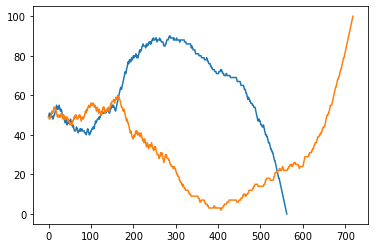
\includegraphics{chapter8/IMG_ch8/pow1N100mu10}
\caption{$\alpha = 1$, $N = 100$, $\mu = 10$. Two realisations of the process. The reversal can clearly been seen in each case.}
\label{2runs}
\end{figure} 

\subsection*{Results}
Running simulations of the model, for now with $\alpha = 1$, we see that the dynamics can indeed resemble what was observed by Pimentel. Both of the two realisations in figure \ref{2runs} display the same kind of behaviour: after some light initial back and forth, one of the populations grows to a position of significant advantage. But it doesn't last. Trained for intraspecific competition, the oppressed population makes a striking comeback, completely overthrowing their adversaries.\par
This was also observed in the experiment; Blowflies come out on top despite initially being pushed to the brink.\\






\noindent
During the last couple of cycles, before fixation, population counts edge ever so close to the boundary. Here, like with the initially critical poise of Fig. \ref{nodisp2runs}, there is a balance between directive forces; resistance of the comparatively supressed population grows to such an extent that the heavy advantage of their adversaries, is muted. And in this arrived at state of poised criticality, like in the previous case, we see a divergence. The two trajectories, as expected, begin to be swayed by subtle underlying disturbances of stochastic undulations.


\begin{figure}[]
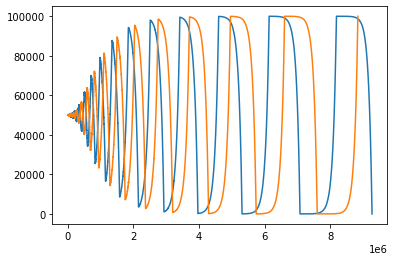
\includegraphics{chapter8/IMG_ch8/pow10N10e5mu1 2 runs 20e3 no displacement}
\caption{$\alpha = 10$, $N = 10\mathrm{e}5$, $\mu = 1$.  Notice that when the two populations start out well-matched, two parallel realizations of the model diverge more substantially than when the initial state involves a bias. Here we see exactly that. The orange and blue lines represent two different stochastic simulations of the model. Because they begin near the critical region of the model, the future trajectory is much more influenced by the cumulative effect of those initial stochastic influences than might otherwise be the case. In the plot below, you can see a red line depicting the critical zone of the model over time. Being near this line is analogous, in deterministic modeling, to having a high Lyapunov exponent.}
\label{nodisp2runs}
\end{figure} 


\begin{figure}[]
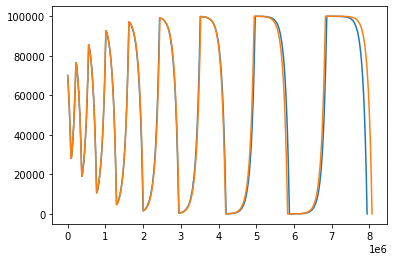
\includegraphics{chapter8/IMG_ch8/pow10N10e5mu1 2 runs 20e3 displacement}
\caption{$\alpha = 10$, $N = 10\mathrm{e}5$, $\mu = 1$.  As mentioned in the caption of the figure above, when trajectories are started with a bias (one species in the majority), repeated simulations will generally stay closer for longer, only diverging near times of extinction. The critical region plays a role in amplifying small differences in stochastic unfolding.}
\label{disp2runs}
\end{figure} 

To get a more clear understanding of what's really going on here we can actually quantify and map this position of criticality over the course of an experiment. By definition, the system is poised at such criticallity exactly when the likelyhood of making a step up vs down is identical:

\begin{equation*}
q_a = \frac{i_c}{N}(1 - p_b) = \left(1 - \frac{i_c}{N}\right) (1 - p_a) = q_b
\end{equation*}
$i_c$ representing the system state at which there is criticality. From this, taking the fact into consideration that $p_a$ and $p_b$ are non-zero with mutual exclusivity, we can derive the relation: 

$$
i_c = 
\begin{cases}
N\dfrac{1 - p_a}{2 - p_a}, &\text{ when } p_a > 0 \text{ and } p_b = 0  \\
N\dfrac{1}{2 - p_b}, &\text{ when } p_b > 0 \text{ and } p_a = 0 \\
\end{cases}
$$

Bearing in mind that $p_a$ and $p_b$ depend on $R_a$ \& $R_b$, and that these are computed as realisations in a stochastic process, the above formulae are not as analytic as they seem. That being said, it is quite straightforward to generate step by step values of the critical state $i_{c, t}$ computationally. These are visible in red over the standard trajectory of the model in figure \ref{redone}. 




\begin{figure}[H]
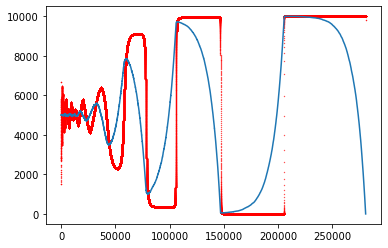
\includegraphics{chapter8/IMG_ch8/pow3N10e4mu1 critical}
\caption{$\alpha = 3$, $N = 10\mathrm{e}4$, $\mu = 1$. The changing critical saddle is depicted in red. When trajectories are close to this line, small perturbations take on a greater significance.}
\label{redone}
\end{figure} 

If we make a qualitative comparrison beteen whats going on in figure \ref{redone}, and in figures \ref{nodisp2runs} \& \ref{disp2runs}, we can see quite clearly, that in \ref{nodisp2runs} \& \ref{disp2runs} trajectories have a propensity to diverge from one another ecaxtly when the state $A_t$ is near criticality.\par
This toughes the essence of what these notes have been trying to get at: near criticality, the future of a system becomes sensitive, succeptible, light underlying stochastic influences. 


\subsection*{Cellular automaton visualisation}

After formulating the model analytically (note: a model has previously been proposed,  \cite{pease1984evolutionary} but the above model wasn't inspired by this and differs in form),  I thought it would be a good idea to produce a spatial version in the form of a sellular automaton. You can see the results of this is the figure here. Blue and red squares represent houseflies and blowflies respectively. This was coded in C++ using the SFML (Simple fast media layer) library which does low-level graphics. 



\begin{figure}[H]
    \centering
    % First row of four images
    \begin{subfigure}{0.22\textwidth}
        \centering
        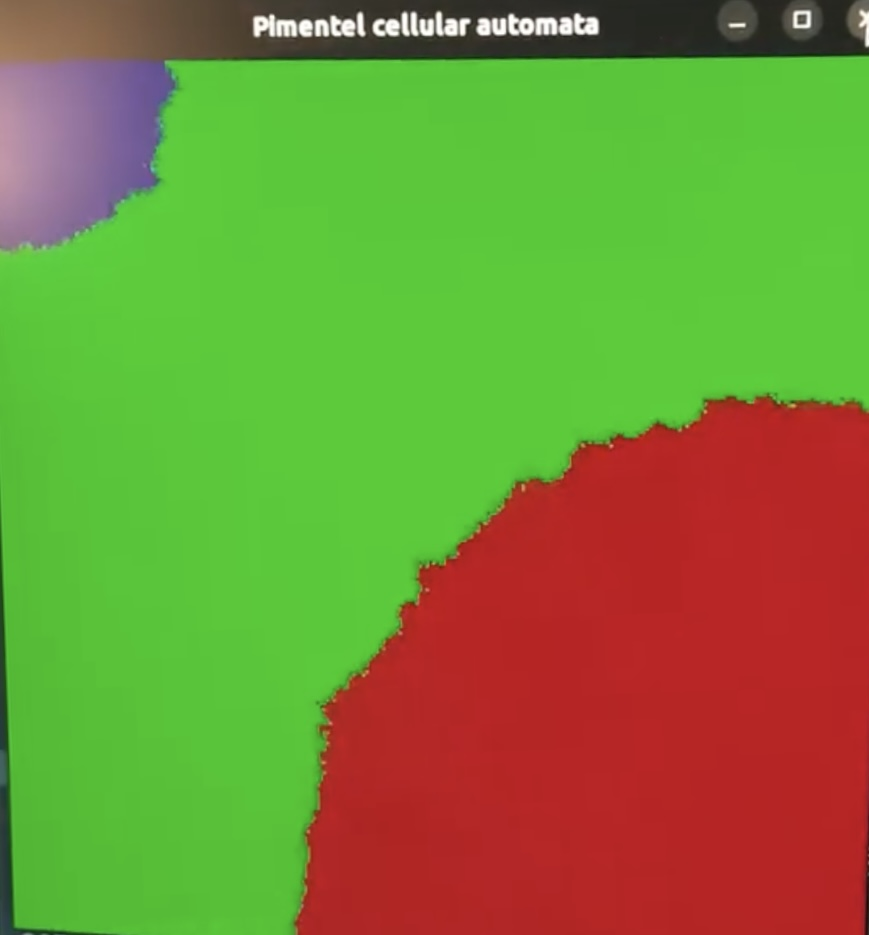
\includegraphics[width=\textwidth]{chapter8/IMG_ch8/pims/pim1.jpg}
    \end{subfigure}
    \hspace{\fill}
    \begin{subfigure}{0.22\textwidth}
        \centering
        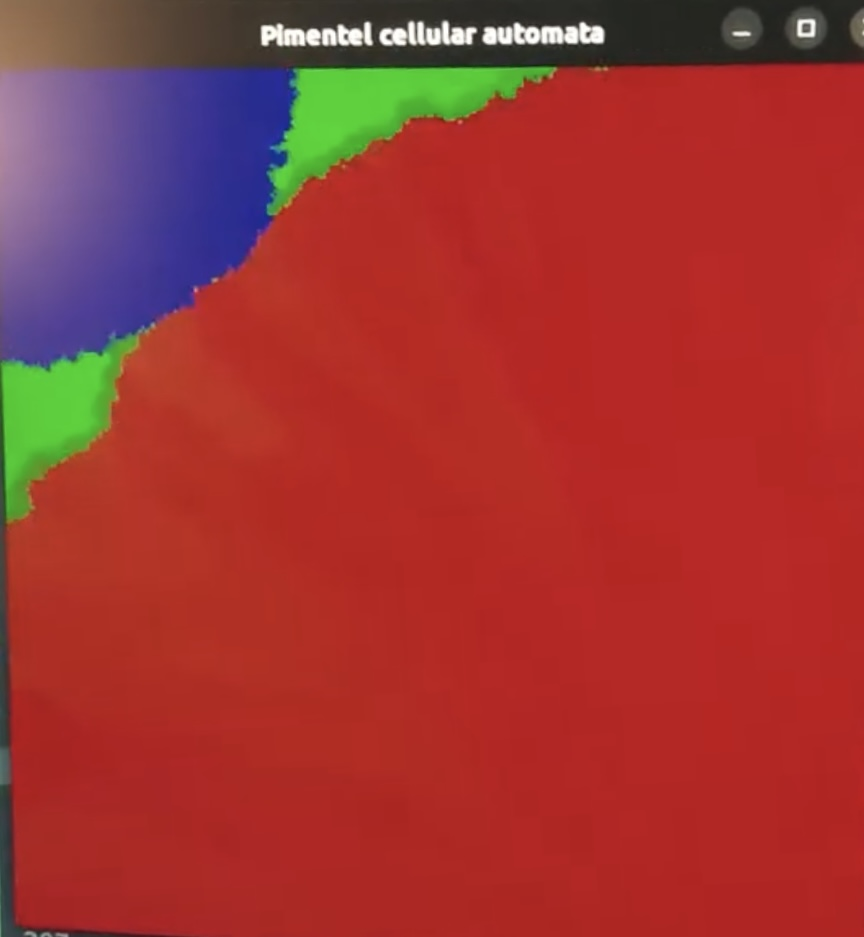
\includegraphics[width=\textwidth]{chapter8/IMG_ch8/pims/pim2.jpg}
    \end{subfigure}
    \hspace{\fill}
    \begin{subfigure}{0.22\textwidth}
        \centering
        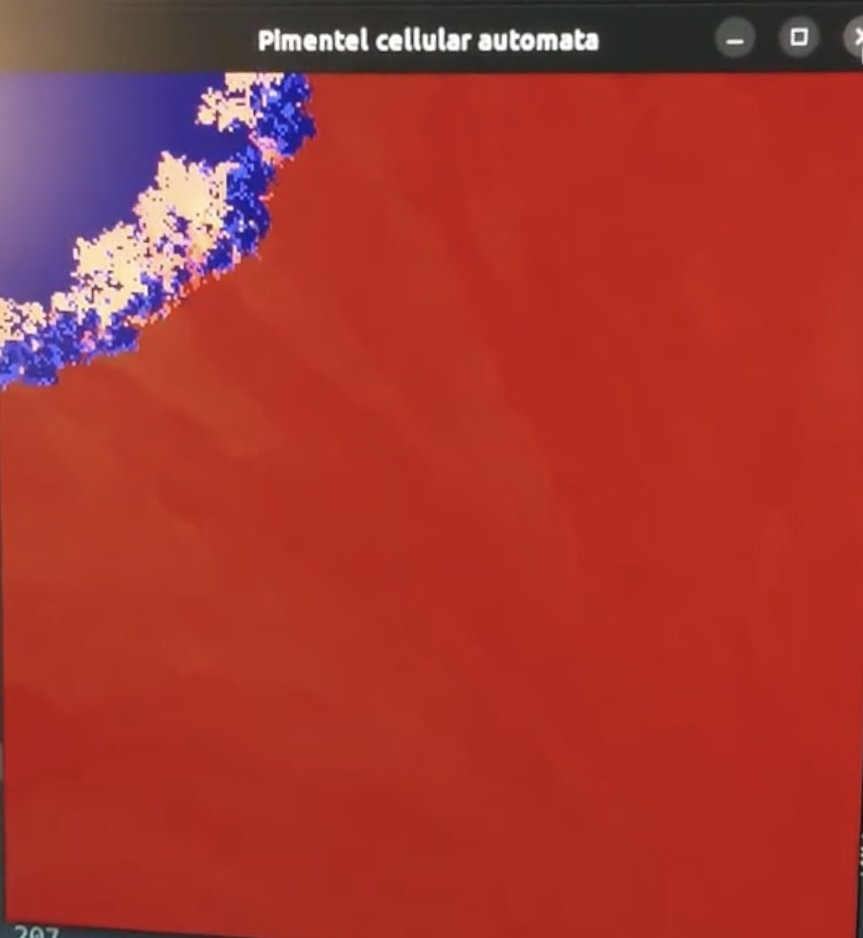
\includegraphics[width=\textwidth]{chapter8/IMG_ch8/pims/pim3.jpg}
    \end{subfigure}
    \hspace{\fill}
    \begin{subfigure}{0.22\textwidth}
        \centering
        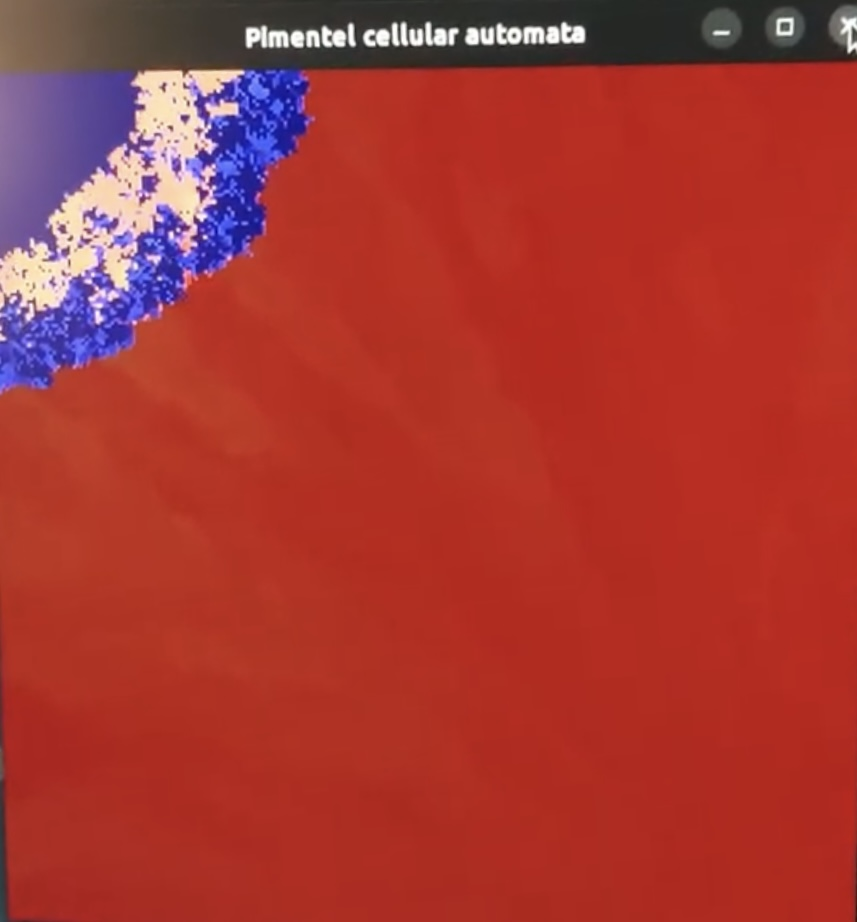
\includegraphics[width=\textwidth]{chapter8/IMG_ch8/pims/pim4.jpg}
    \end{subfigure}
    
    \vspace{0.5em} % Small vertical space between rows

    % Second row of four images
    \begin{subfigure}{0.22\textwidth}
        \centering
        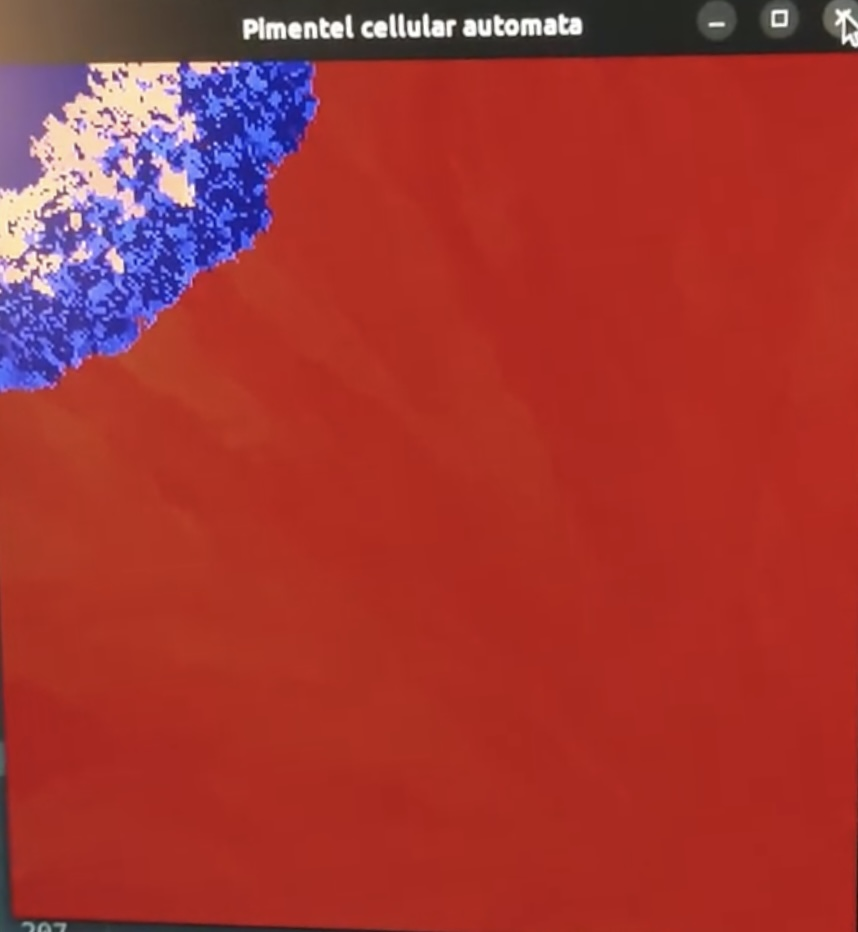
\includegraphics[width=\textwidth]{chapter8/IMG_ch8/pims/pim5.jpg}
    \end{subfigure}
    \hspace{\fill}
    \begin{subfigure}{0.22\textwidth}
        \centering
        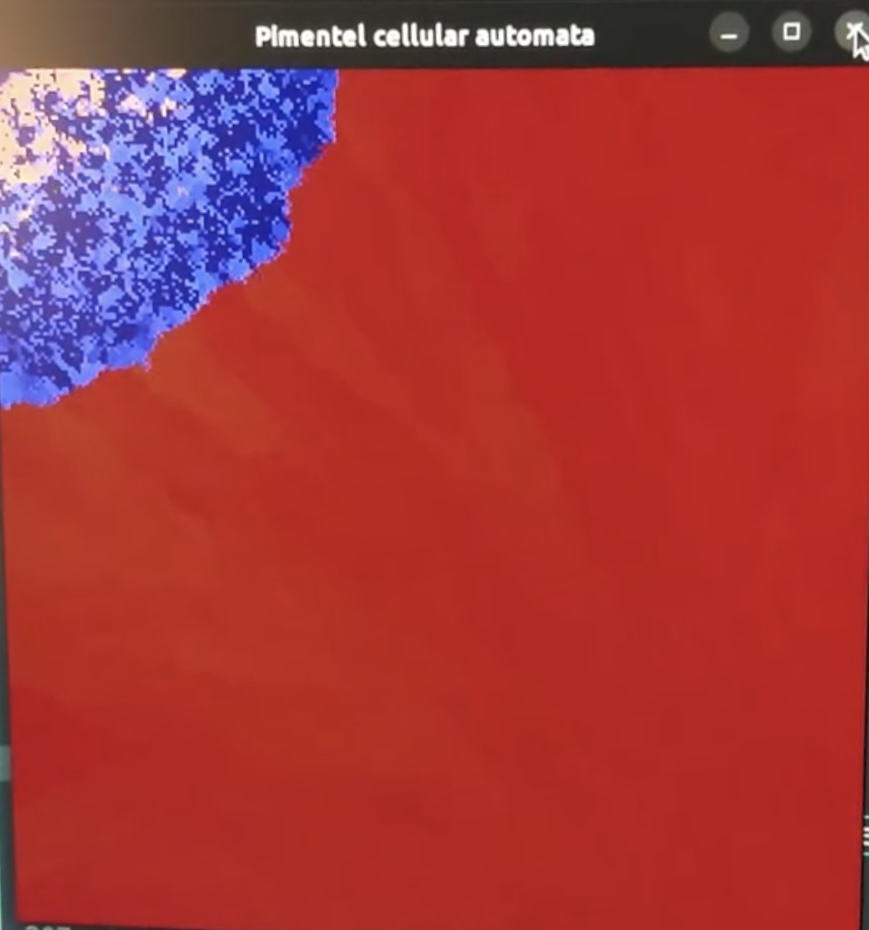
\includegraphics[width=\textwidth]{chapter8/IMG_ch8/pims/pim6.jpg}
    \end{subfigure}
    \hspace{\fill}
    \begin{subfigure}{0.22\textwidth}
        \centering
        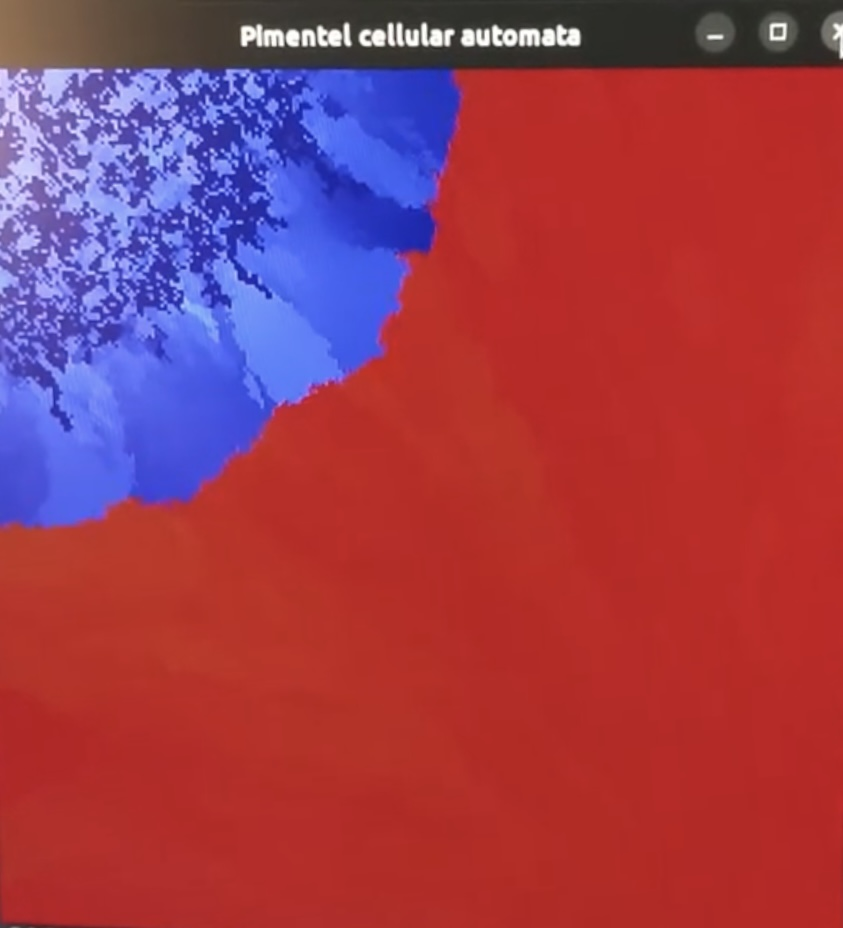
\includegraphics[width=\textwidth]{chapter8/IMG_ch8/pims/pim7.jpg}
    \end{subfigure}
    \hspace{\fill}
    \begin{subfigure}{0.22\textwidth}
        \centering
        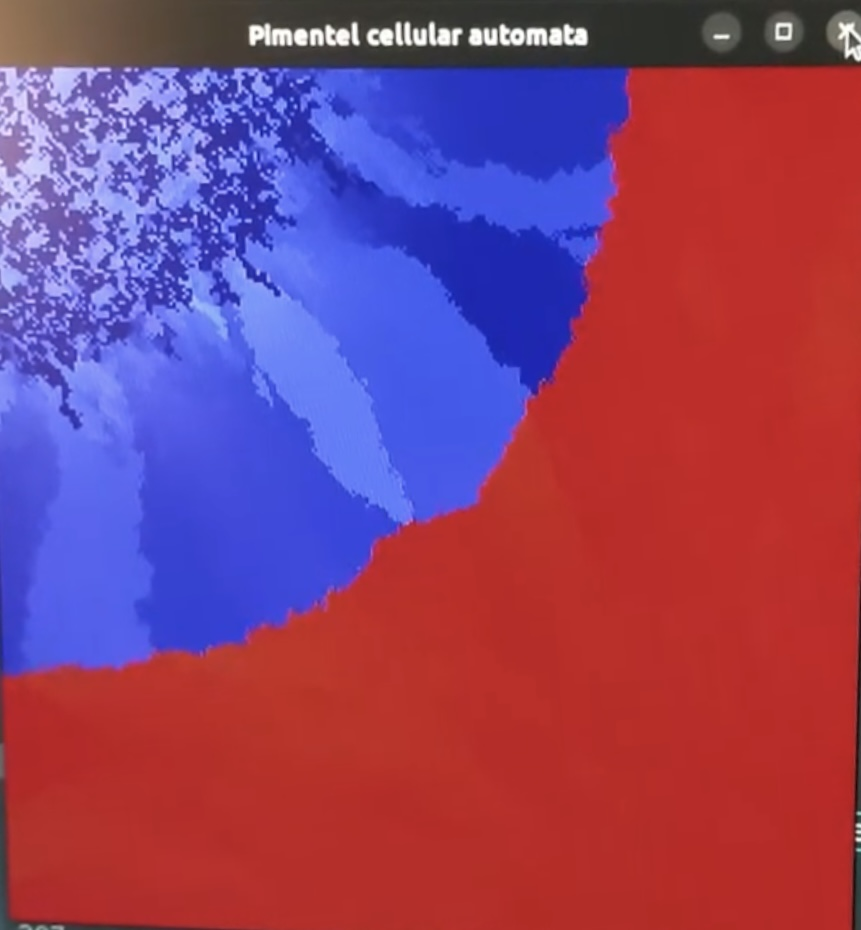
\includegraphics[width=\textwidth]{chapter8/IMG_ch8/pims/pim8.jpg}
    \end{subfigure}

    \vspace{0.5em} % Small vertical space between rows

    % Third row of three images
    \begin{subfigure}{0.22\textwidth}
        \centering
        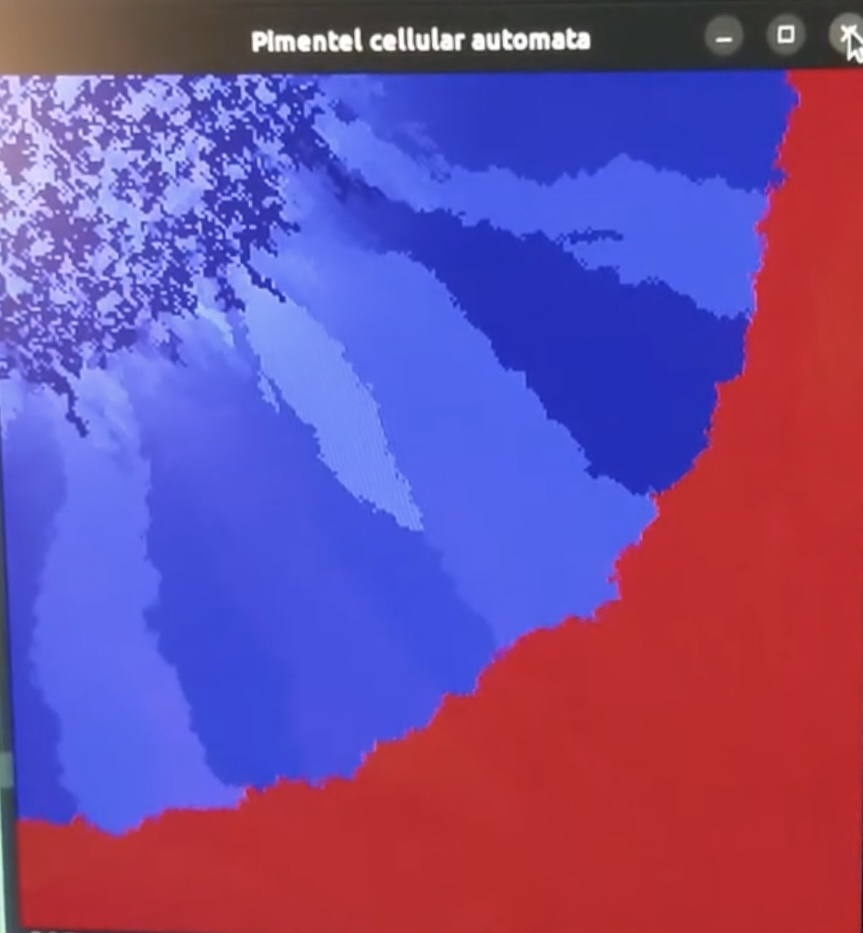
\includegraphics[width=\textwidth]{chapter8/IMG_ch8/pims/pim9.jpg}
    \end{subfigure}
    \hspace{10pt}
    \begin{subfigure}{0.22\textwidth}
        \centering
        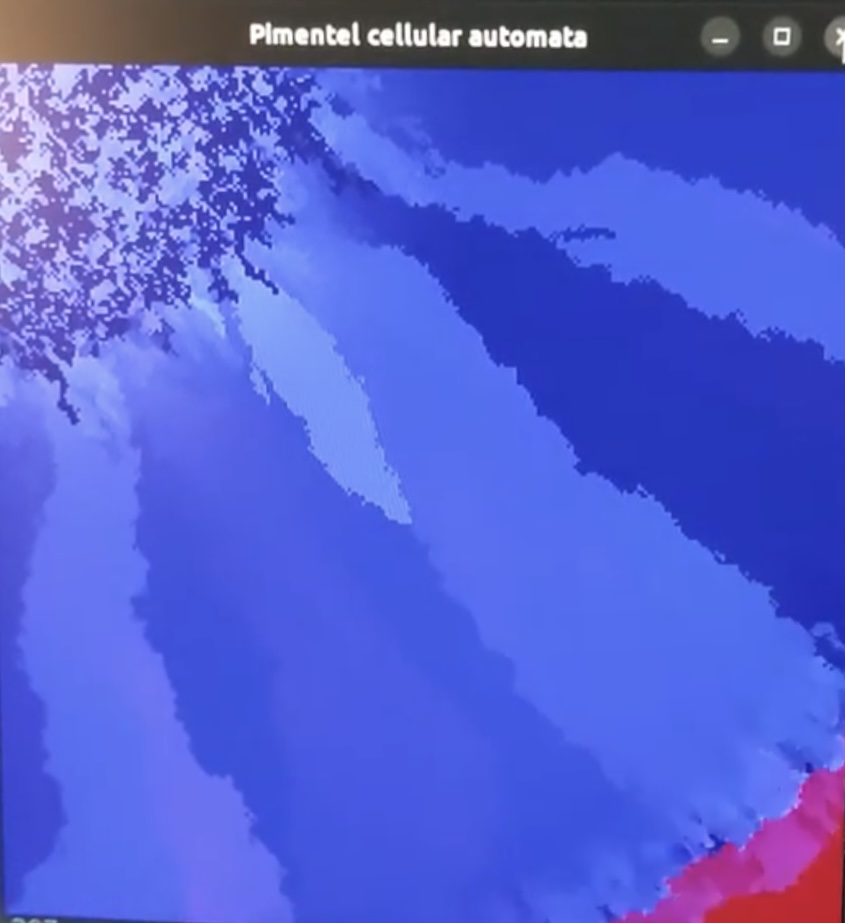
\includegraphics[width=\textwidth]{chapter8/IMG_ch8/pims/pim10.jpg}
    \end{subfigure}
     \hspace{10pt}
    \begin{subfigure}{0.22\textwidth}
        \centering
        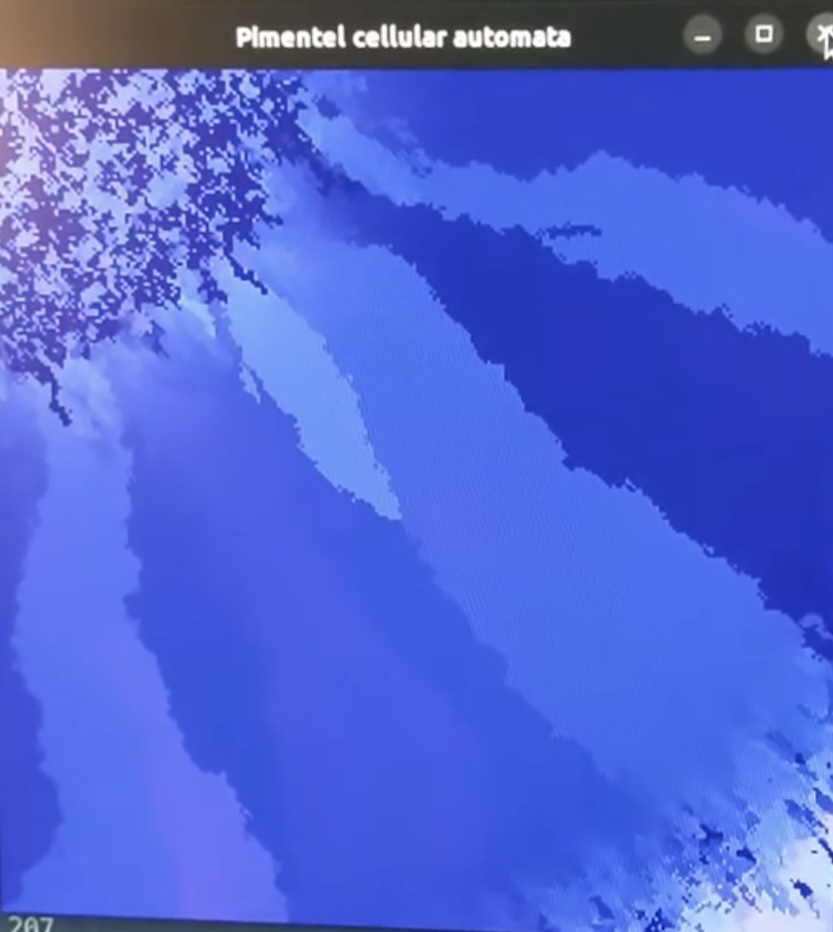
\includegraphics[width=\textwidth]{chapter8/IMG_ch8/pims/pim11.jpg}
    \end{subfigure}

    % Single caption for all images
    \caption{Picured above is a series of frames from an animation: a spatial cellular automaton version of the pimental model. You can see that the initial advantage of the red population is cast aside by the blues after they become hardened and more competetive following intraspecific interactions. The shades within each population only depict relative heredity and don't have any bearing on the dynamics. }
    \label{fig:sequential_images}
\end{figure}











































\subsection{Pimental +}


\noindent
It might be possible to use the pimental model to frame a description of a hypothetical link between speciation and population collapse. An endogeneous process in which the unleasing of variation (facilitated by favourable conditions), can ultimately lead to the demise of a population, as other groups rise to dominance. This process is an attempt to mathematisize what Nietzcche described alegorically in words: the process by which group variation results from favourable circumstances, but how this itself can lead to failiure through a weakining of established forms. The following quote is from``Beyond good and evil'' section 262 \cite{nietzsche2013beyond}:


\begin{quotation}
``A species originates, and a type becomes established and strong in the long struggle with
essentially constant unfavourable conditions. On the other hand, it is known by the experience of
breeders that species which receive super-abundant nourishment, and in general a surplus of
protection and care, immediately tend in the most marked way to develop variations, and are
fertile in prodigies and monstrosities (also in monstrous vices). Now look at an aristocratic
commonwealth, say an ancient Greek polis, or Venice, as a voluntary or involuntary contrivance
for the purpose of rearing human beings; there are there men beside one another, thrown upon
their own resources, who want to make their species prevail, chiefly because they must prevail,
or else run the terrible danger of being exterminated. The favour, the super-abundance, the
protection are there lacking under which variations are fostered; the species needs itself as
species, as something which, precisely by virtue of its hardness, its uniformity, and simplicity of
structure, can in general prevail and make itself permanent in constant struggle with its
neighbours, or with rebellious or rebellion-threatening vassals. The most varied experience
teaches it what are the qualities to which it principally owes the fact that it still exists, in spite of
all Gods and men, and has hitherto been victorious: these qualities it calls virtues, and these
virtues alone it develops to maturity. It does so with severity, indeed it desires severity; every
aristocratic morality is intolerant in the education of youth, in the control of women, in the
marriage customs, in the relations of old and young, in the penal laws (which have an eye only
for the degenerating): it counts intolerance itself among the virtues, under the name of "justice."
A type with few, but very marked features, a species of severe, warlike, wisely silent, reserved,
and reticent men (and as such, with the most delicate sensibility for the charm and nuances of
society) is thus established, unaffected by the vicissitudes of generations; the constant struggle
with uniform unfavourable conditions is, as already remarked, the cause of a type becoming
stable and hard. Finally, however, a happy state of things results, the enormous tension is
relaxed; there are perhaps no more enemies among the neighbouring peoples, and the means of
life, even of the enjoyment of life, are present in super abundance. With one stroke the bond and
constraint of the old discipline severs: it is no longer regarded as necessary, as a condition of
existence--if it would continue, it can only do so as a form of luxury, as an archaising taste.
Variations, whether they be deviations (into the higher, finer, and rarer), or deteriorations and
monstrosities, appear suddenly on the scene in the greatest exuberance and splendour; the
individual dares to be individual and detach himself. At this turning-point of history there
manifest themselves, side by side, and often mixed and entangled together, a magnificent,
manifold, virgin-forest-like up-growth and up-striving, a kind of tropical tempo in the rivalry of
growth, and an extraordinary decay and self-destruction, owing to the savagely opposing and
seemingly exploding egoisms, which strive with one an other "for sun and light," and can no
longer assign any limit, restraint, or forbearance for themselves by means of the hitherto existing
morality. It was this morality itself which piled up the strength so enormously, which bent the
bow in so threatening a manner:--it is now "out of date," it is getting "out of date." The
dangerous and disquieting point has been reached when the greater, more manifold, more
comprehensive life is lived beyond the old morality; the "individual" stands out, and is obliged to
have recourse to his own law-giving, his own arts and artifices for self-preservation, self-
elevation, and self-deliverance. Nothing but new "Whys," nothing but new "Hows," no common
formulas any longer, misunderstanding and disregard in league with each other, decay,
deterioration, and the loftiest desires frightfully entangled, the genius of the race overflowing
from all the cornucopias of good and bad, a portentous simultaneousness of Spring and Autumn,
full of new charms and mysteries peculiar to the fresh, still inexhausted, still unwearied
corruption. Danger is again present, the mother of morality, great danger; this time shifted into
the individual, into the neighbour and friend, into the street, into their own child, into their own
heart, into all the most personal and secret recesses of their desires and volitions. What will the
moral philosophers who appear at this time have to preach? They discover, these sharp onlookers
and loafers, that the end is quickly approaching, that everything around them decays and
produces decay, that nothing will endure until the day after to-morrow, except one species of
man, the incurably mediocre. The mediocre alone have a prospect of continuing and propagating
themselves--they will be the men of the future, the sole survivors; "be like them! become
mediocre!" is now the only morality which has still a significance, which still obtains a hearing.--
But it is difficult to preach this morality of mediocrity! it can never avow what it is and what it
desires! it has to talk of moderation and dignity and duty and brotherly love--it will have
difficulty in concealing its irony!''
\end{quotation}

The basic pimental model as defined above encorporates the fitness of two populations, these increasing when the particular species is pushed into a minority. 

$$\pr{\Delta A_t = 1} = \frac{A_t}{N} \frac{f_a}{\bar f}$$

$$\pr{\Delta A_t = 1} =\lrb{ 1 - \frac{A_t}{N}} \frac{f_b}{\bar f}$$




where $A_t$, $B_t$, and $N$ represent the relative domination of group $A$, group $B$, and the total domain capacity. With the Moran assumption, $A_t = N - B_t$. Like above, these are essentially the probabilities of a chosen individual encountering a member of the opposite group ($A_t/N$) \textbf{and} defeating them in competition ${f_a}/{\bar f}$. In this unaltered model, fitness changes according to

$$f_a(t+\Delta t) = f_a(t) + \delta \lrb{\frac{B_t}{A_t}}^\alpha$$

$$f_b(t+\Delta t) = f_b(t) + \delta \lrb{\frac{A_t}{B_t}}^\alpha$$

\noindent
Note: this is a slightly different definition to the one shown above. $R_a$ \& $R_b$ are replaced by $f_a$ \& $f_b$, but the dynamics are at least qualitativaly identical. 

\subsubsection*{Sub-species, including variable speciaton}

Suppose we incorporate a species count for each population, $\xt^{(a)}$ and $\xt^{(b)}$, respectively. According to the alagory laid out by neitche, exxessive variation (the emergence of many species), leads to a weakening of a population. In our model, that would be represented by a drop in fittness. But how does the number of species change. Generally speaking, variation will increase when the demands of survival are lessened by favourable circumstances. In our model, something like this will be represented by the product of domain control and fitness.\par 
Take for example

$$\pr{\Delta \xt^{(a)} = 1}  = \beta_a\xt^{(a)} \Delta t$$

$$\pr{\Delta \xt^{(a)} = -1}  = \mu_a\xt^{(a)} \Delta t$$

\noindent
with extinction $\mu_a$ constant, and speciation $\beta_a$ varing according to fitness, $f_a$, and relative domination $(A_t / N)$:

$$\beta_a = \lrb{\frac{A_t}{N}}^\lambda f_a$$ 

\noindent
The dynamics for the other species count $\xt^{(b)}$ would function in the same way but with $A_t$ being replaced by $B_t$ etc... 

\subsubsection*{Effect of species count on fitness}

\noindent
Then there is the effect of excess variation on reducing a group's fitness.Something like this could serve well,

$$f_a(t+\Delta t) = f_a(t) + \delta \lrb{\frac{B_t}{A_t}}^\alpha  - \gamma \xt^{(a)}$$

$$f_b(t+\Delta t) = f_b(t) + \delta \lrb{\frac{A_t}{B_t}}^\alpha  - \gamma \xt^{(b)}$$

\noindent
with constant $\gamma$ representing the abount by which the inneficencies of excess variations weigh on overall performance. \par 

\subsubsection*{Comments}
Unfortunately, for this model, along with half a dozen other speculative models relating to speciation and evolution, I didn't get round to running simulations or doing much analysis. This is inevitable. and the model outlined here is itself a description of why. Models, like any other form of coded information are subject to the laws of variation whereby one model, on creative consideration, soon gives birth to many more. And with time and energy resources being limited, a multiplicity like this hs the effect of spreading resources more thinly, each gets less and less attention as the number increases. And before you know it, its time to write a thesis, and most of them get discarded.\par
But I thought, I'd at least write this one down, because it contains my best attempt at describing mathematically the endogeneous aspect of collapse by variation.  


















\section{Allegorical model of rise run ruin rejuvenation}


I wanted to try to represent a certain style of stochastic cyclic dynamics. A pattern in which potential (energy) builds up constantly in the absence of use.  Then in surplus, the count of individual agencies (species) increases in response to the excessive energy potential. \par 
The potential is diminished by the large number of agencies until at some time,  a state of scarcity comes about. And in this, there is a catastrophic extinction in which all of the agencies die. In reality, not all of the agencies (species) will die, some will remain and become distinct in the newly hash selective conditions. \par 
From here, the cycle repeats. Potential once more begins to build until a Poission revival kickes off a new proliferative wave.  Yes, in reality, this will begin from one or a few of the agencies  remaining beyond the catastrophe. \par




\noindent
The purpose of this model is to make some link between a potential dynamics in the cyclic rise and decline of dissipative structures in the context of a constant supply of energy.  We perhaps see this style of dynamics both in the cyclic dynamics of turbulance shedding in the Stokes flow around a circle, and the periodic rise and collapse of ecosystems and even cultures. 

\subsection*{Model specification}

% Just notes, not final

(Energy availability)
 $$\ddt{N} = \xi - \mu \xt$$
(Segregation into multiplicity)
$$\pr{\Delta \xt = 1} = \lambda \xt \delt + o(\delt)$$
(Catastrophic collapse)
$$\pr{\xdt = 0 | \xt} =  \delta \frac{\xt}{N(t)} \delt +o(\delt)$$
(Poisson revival)
$$\pr{\xdt = 1 | \xt = 0} = \alpha \delt + o(\delt)$$
(No event)
$$\pr{\xdt = \xt} = 1 - \lrb{\lambda \xt  + \delta \frac{\xt}{N(t)} + \alpha   }\delt + o(\delt)$$





\begin{figure}[H]
    \centering
    % First figure
    \begin{subfigure}{0.48\textwidth}
        \centering
        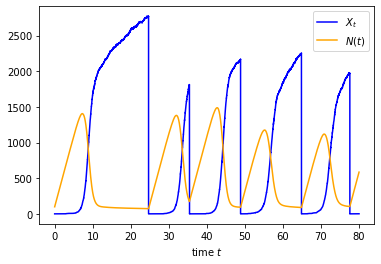
\includegraphics[width=\textwidth]{chapter8/IMG_ch8/VBCfigs/80for1VBC} % Adjust the image path as necessary
    \end{subfigure}
    \hspace{\fill} % Optional: adds space between figures
    % Second figure
    \begin{subfigure}{0.48\textwidth}
        \centering
        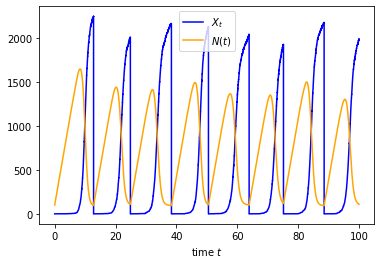
\includegraphics[width=\textwidth]{chapter8/IMG_ch8/VBCfigs/100for1VBC} % Adjust the image path as necessary
    \end{subfigure}
    
    \caption{Realisations of the model.  Potential energy, $N(t)$,  shown in orange, agency count,  $\xt$, in blue.}
    \label{fig:two_figures}
\end{figure}



\begin{figure}[H]
    \centering
    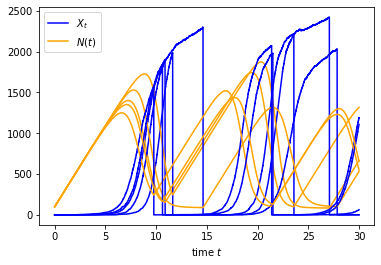
\includegraphics[width=0.7\textwidth]{chapter8/IMG_ch8/VBCfigs/30for5VBC} % Adjust the width as needed
    \caption{Multiple realisations with the same parameters and initial condition.}
    \label{fig:single_figure}
\end{figure}









\noindent
$\xt$, the replicative units (or objects of multiplicity in segregation) can be thought to represent a great many different things. They may be framed as the individuals in a population; of bacteria, viruses, organisms. They may be species within a genre, fractured but internally coherent groups within a broader population. Autonomous agencies within an organisation --- this is quite a general concept and could be applied to a number of situations: teams in a company, parties in a political system. A great many things can be placed in these terms... It would be fair to say that some of these representations are loose and ill-defined. But there is a more general way of looking at it, at what the quantity $\xt$ is attempting to capture. It's a proxy for order. That is, negative entropy. Think for a moment of a further analogy in fluid flows. If we observe the transition form laminar flow to turbulence, there is a fragmenting of flow directions. At first, all streamlines point in one onwards direction of motion. At the end of the transition, there are what appears to be an infinitude of ever more minute and fleeting divergences; of flow-lines separating off from one-another.\par



Admittedly, this does happen in spatial continuum rather than discrete jumps. But say for a moment we were to view this degenerative separation at a course grain. We might see from the outset an initial branching into two distinct pathways. Each of which encompassing fluid flow of roughly coherent direction. Each of these then has the potential to further subdivide into two. And each time this breakage takes place, there is further dissipation. In our coarse approximate description, there are a greater number of flow interfaces --- more locations of friction. Each sub-stream, smaller and smaller in cross-section will carry less and less kinetic energy and a greater proportion of the energy will be lost as heat.\par 
Towards the limit, minute, infinitely multiplicitous and scattered fluid trajectories will become so energy lacking as to resemble little more than stationary fluid. 
From here, with ongoing general flow, there will be a re-cohering into a more broadly aligned fluid stream. This, then, will likely be seen to once more progress in a dissipative turbulent divergence as before. In this way, a kind of oscillation commences. From Laminar, to turbulent, and through fizzling out, back to laminar, turbulent, so on and so forth. 

In real fluid flows --- take for example flow around a circle (or sphere in three dimensions) --- the oscillation is not absolute; both more turbulent and less turbulent regions coexist in an oscillatory spatial continuum. Laminar flow begins to shed turbulence as it sways one way in the wake of the circle; then going on to drift back into where the turbulence last was.\par 


Let us turn to another example of a dissipative structure: the fragmenting of a genus population into species over large swathes of time. That this is an example of a Prigoginian dissipative structure is a claim worth scrutinizing. I do believe it has been made before by others \cite{elitzur1994let} \cite{sharma2023assembly}.  None the less, let us be careful. 

Living organisms are one of the most rapidly dissipating arrangements in the universe. It has been observed that per kilogram, humans and other terrestrial life forms dissipate energy as a rate orders of magnitude greater than the sun. They are also highly ordered, local low-entropy formations which are kept far above equilibrium by their continual usage of energy. So it seems natural to assign the term ``dissipative structure'' to living organisms taken at the individual level. 
But can we speak more generally about life and its natural progressions? Over time, genera fragment into species. It seems straightforward that this is an example of entropy reduction.  



\vspace{10pt}

\hrule

\vspace{10pt}



\noindent
\textbf{Aside:} In "The genetical theory of natural selection" (1930),  R.  Fisher makes mentions something in relation to this line of thought: 

\begin{quote}
\noindent
"A philospohical view of history, which has attained to great popularity in several continental countries,  regards the rise as well as the fall of civilisations as but successive phases of a cycle of growth and decay,  which, it is supposed, repeats itself endlessly,  throughout human history.  So long as we aim at no more than an effective generalised description of the phenomena there is much to be said for considering the phases of rise and development of the great civilisations in conjunction with the phases of their decayand collapse. It is a real advantage that the parallelisms between the earlier phases of different cultures should be recognised, and that their relations in time to recognizably parallel later phases should be established as accurately as possible.  Generalised description should, however,  never be regarded as an aim in itself."
\end{quote}

"Generalised description should, however,  never be regarded as an aim in itself" -- maybe I should have read this before working on the equations above.  But perhaps there is a certain utility in the aesthetic of a generalised description when it becomes codified in the language of a mathematical model. 




\vspace{10pt}

\hrule


\vspace{10pt}





\section*{Bardo Thodol}

 In the Bardo Thodol (otherwise known as The Tibetan book of living and dying), there are listed 6 bardo states which describe the stages of life and the process of transition between lives:

\begin{itemize} \item the bardo of birth \item the bardo of dreams \item the bardo of samadhi meditation \item the bardo of the moment before death \item the bardo of dharmata (pure reality) \item the bardo of becoming \end{itemize}

I can't help but notice a crossover with the first three of these and the stages of the Mandukya Upanishad: A, U, and M for "beginning," "process," and "cessation." This links loosely with the stages of the logistic growth model. Initially, the number of species rapidly increases, then there is a stabilizing phase, and eventually, many die out, leaving only a few. But this is an aside.

The point of the Bardo Thodol demonstrates an understanding of something also revealed by stochastic process theory: that in life, there are periods of relative stasis punctuated by times of great upheaval, change, and above all, uncertainty. The book is a guide for those dying, so that they may pass through the crucial final three stages to attain a favorable passage through the period of undetermined futures. The idea is that their consciousness somehow persists after their physical body dies. It then wanders through the bardo of dharmata, before stumbling upon a series of lights. Each light encountered corresponds to one of the 6 realms of samsara in which the person might find themselves born.

\vspace{5pt} \hrule \vspace{5pt}

\noindent \textbf{Aside -- the 6 realms of samsara: } In Tibetan Buddhist theory, there are 6 "realms" in which all beings supposedly occupy, cycling among them over a series of cycles of birth, death, and rebirth:

\begin{itemize} \item Hell realm(s) \item Animal realm \item Realm of hungry ghosts \item Human realm \item Realm of the jealous gods \item Deva realm \end{itemize}

The stated ideal is to, as it were, exit this process of cycles and become "enlightened." This can only happen at the time of death and supposedly is most easily accomplished when exiting the human realm. The trick is to use the opportunity of non-fixation to remain in the state of transience without falling back into one of the realms, and it is this which the Bardo Thodol aims to guide its recipients towards.

\vspace{5pt} \hrule \vspace{5pt}

The lights seem to be analogous to circumstances that seem appealing but end up as "basins of attraction," whereby entry inevitably leads to an absorption and fixation in that particular realm. There is a clear analogy to observations in stochastic process analysis. For example, at a state of undetermined instability (as in the squeezes that take place when one population is very small in the Pimental model), nearby trajectories diverge as a result of an amplification in the importance of small, otherwise insignificant, stochastic influences.

In this framework, when a person dies, their fated trajectory is yet undecided, and in this state of undetermined instability, small influences can be applied to steer things one way or the other.

\subsubsection*{Why do we care?} In the modern scientific age we live in, most educated people balk and sneer at the concept of life after death.  There appears two angles through which to address the matter:

\begin{itemize} \item \textbf{You could say that there are many lives within one life}, and that the transition between phases of life shares qualities with the stated transition between the bardo of the moment before death and the bardo of becoming. In a way, I feel as if I am embarking on the bardo of the moment before death.  The path of life after a PhD, without concrete plans, can be underermined and subject to an array of possible continuations. 

\item (More abstractly) \textbf{Multiple successive individual people can occupy the same character.} It can be imagined that this effect will have been all the more pronounced in 9th-century Tibet. For centuries, over countless generations, families will have occupied the Tibetan plateau in relative isolation. With this slowed movement, it seems only natural that the perception of rise, fall, and change will have been extended to perceive the agencies living over multiple generations. Take as a prime example the "character" of the Dalai Lama and the continuously reincarnated lamas of the other major schools: one personality, living over 10 or more generations.

New head lamas are selected at birth. They are identified by the elders of the school to be the "reincarnation" of the previous leader. It strikes me as a remarkable mechanism of government for creating piety and meritous behaviour amongst a people: give everyone's child the prospect of becoming leader of the state.

\end{itemize}

\subsection*{Quasistationarity} 

Verging a bit into the reckless and speculative here.  But is there not a philosophical analogy between quasistationarity --- that is,  quantified behaviour of a stochastic process given non-fixation --- and the theoretical description of liberation in the conception of the Bardo Thodol. \par 
Not getting stuck in one of the basins of attraction of the 6 realms, appears similar to not getting stuck, either by depletion to 0 or by catastrophic fixation in the birth death catastrophe process.  Similar to Icarus, neither flying too high or too low,  the liberatee of the bardo of dharmata doesn't get too close to any of the appealing absorbative attractions which would inevitably lead to a re-binding into one of the cyclic domains of samsara.  \par 
Behavior conditional on non-fixation, non rebirth --- that being the practive of the Arahant as that of the Bodisatva.  Unbound and unmarred by conditions of suffering which arise from the succeptability of craving for material manifestations. \par 





\begin{figure}[H] 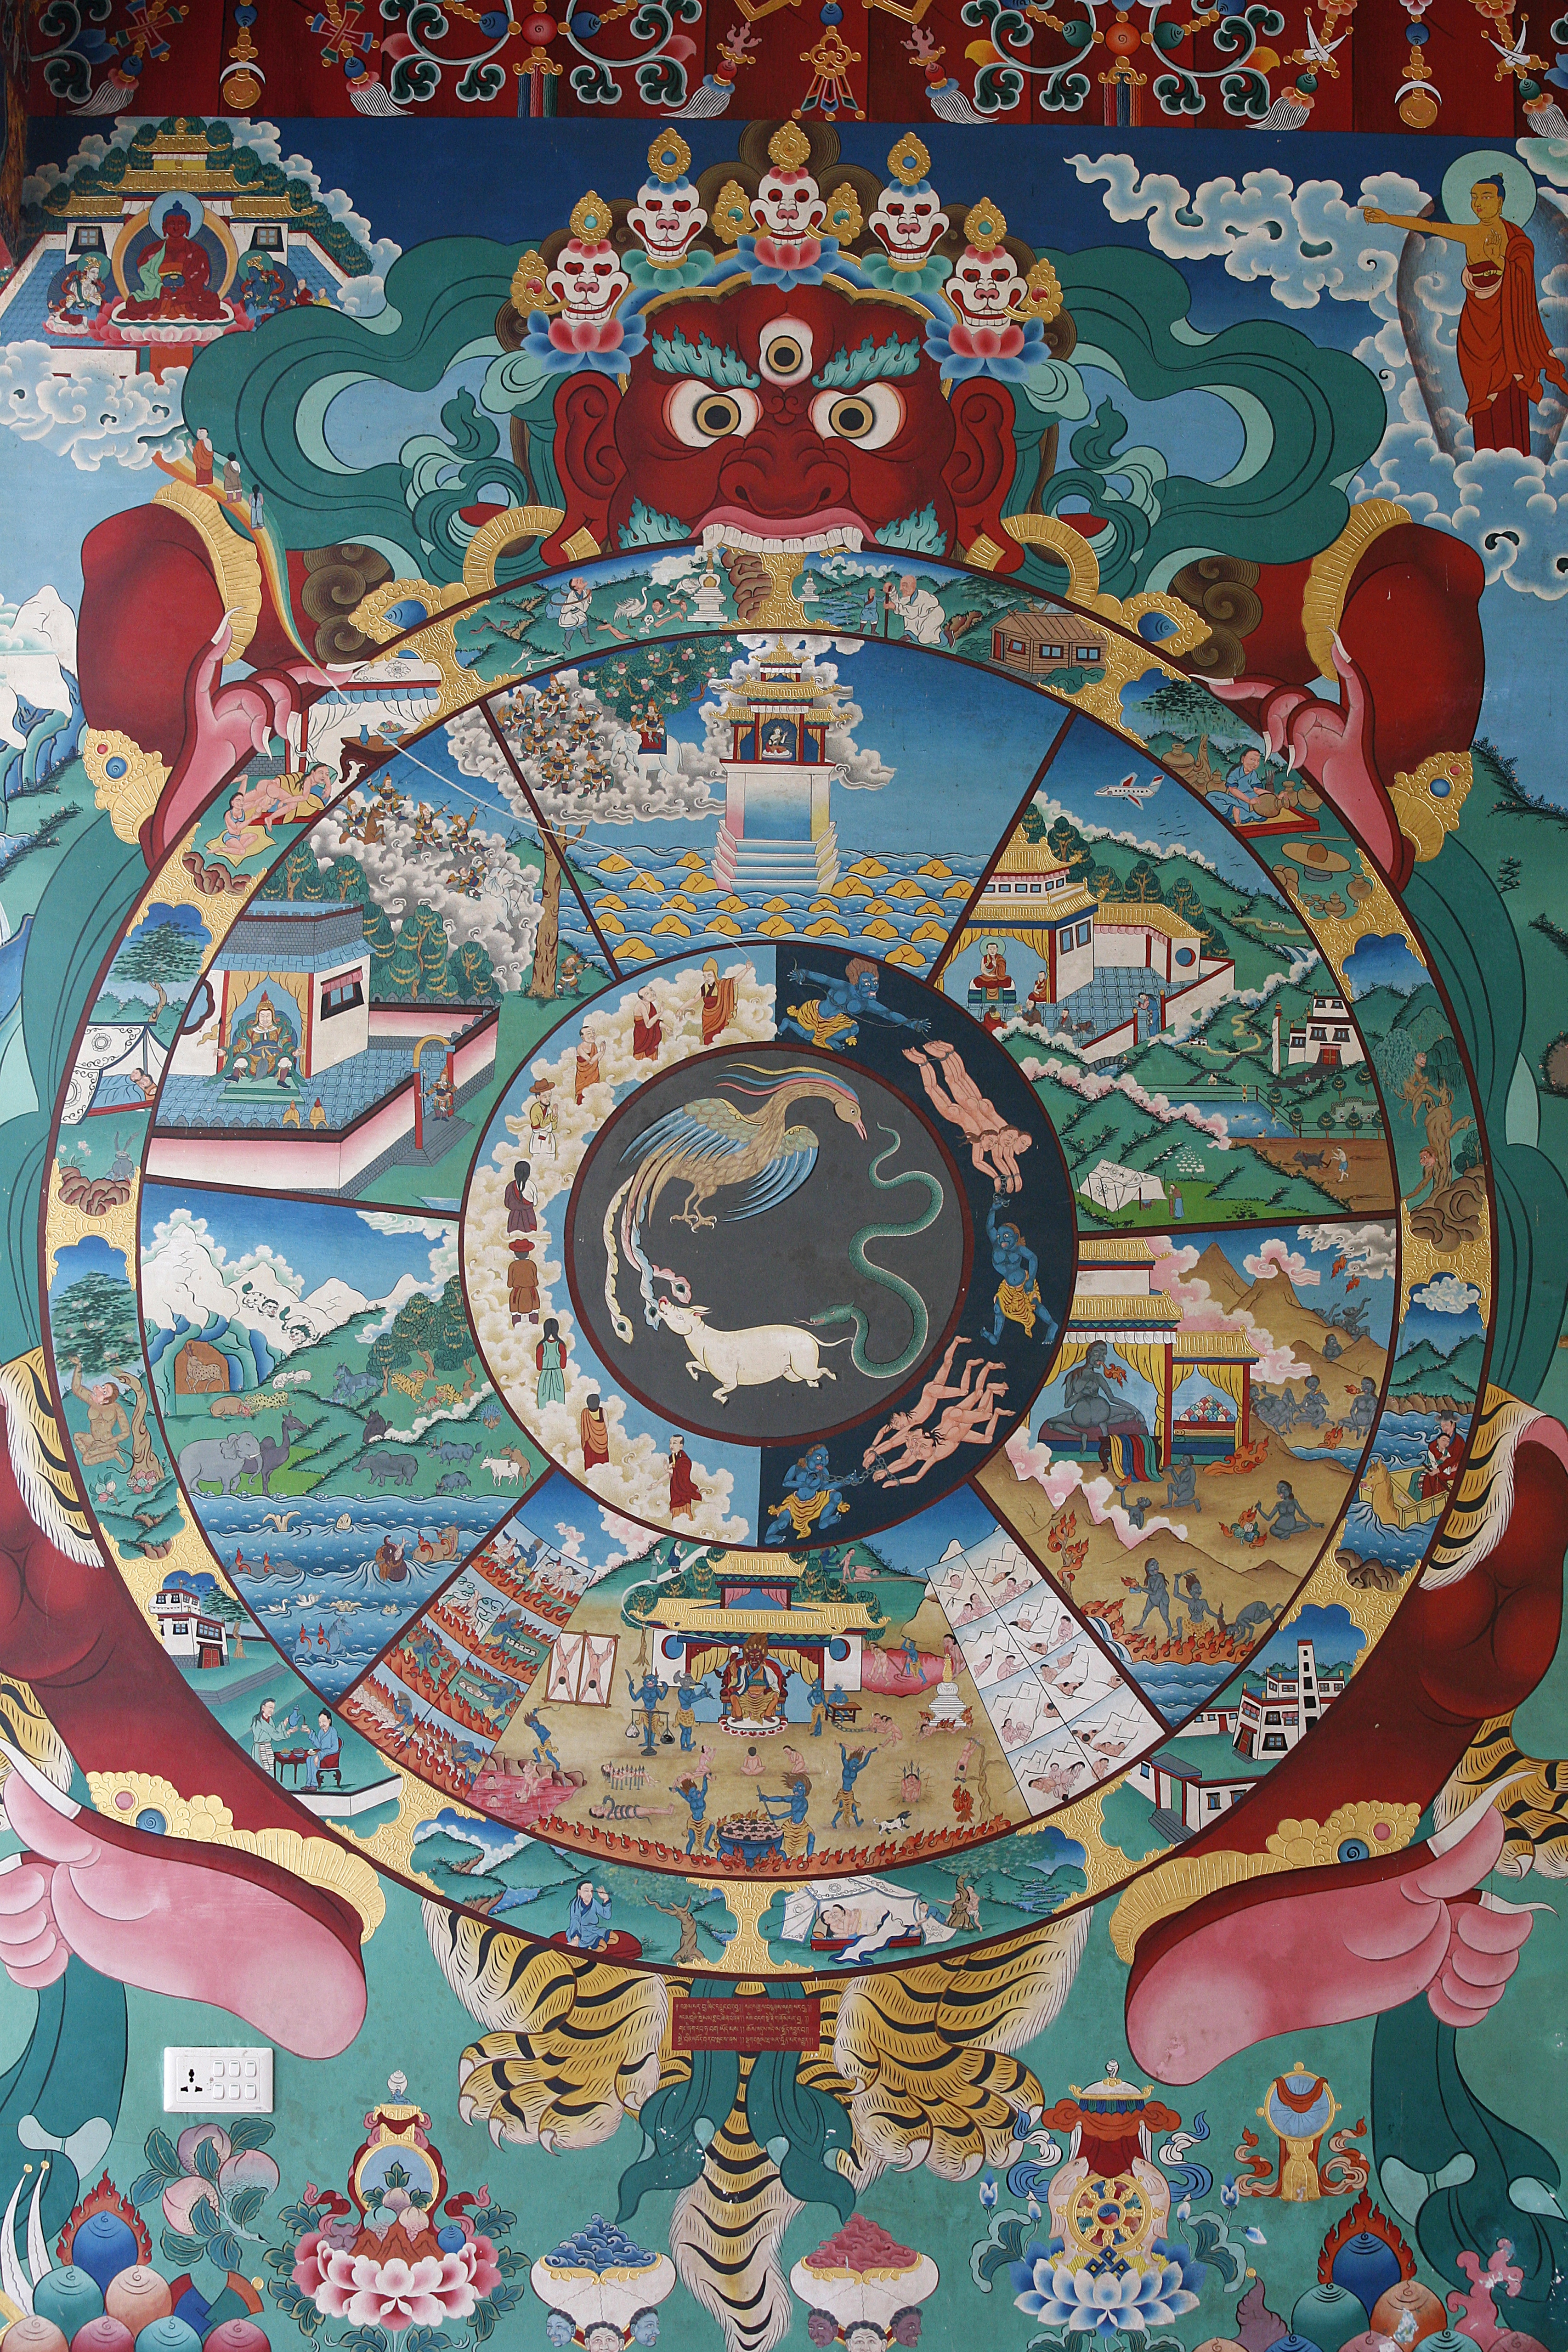
\includegraphics[width = 0.85\textwidth]{chapter8/IMG_ch8/samsara.jpg}
\centering
\pagebreak \caption{Wheel of samsara. Yama (god of death) depicted holding a wheel containing the 6 realms. From the center, a rooster, snake, and pig are shown to represent attachment, aversion, and ignorance respectively. They are said to link with one another cyclically, causing the dynamism which makes the wheel progress.} \label{redone} \end{figure}

\begin{figure}[H] 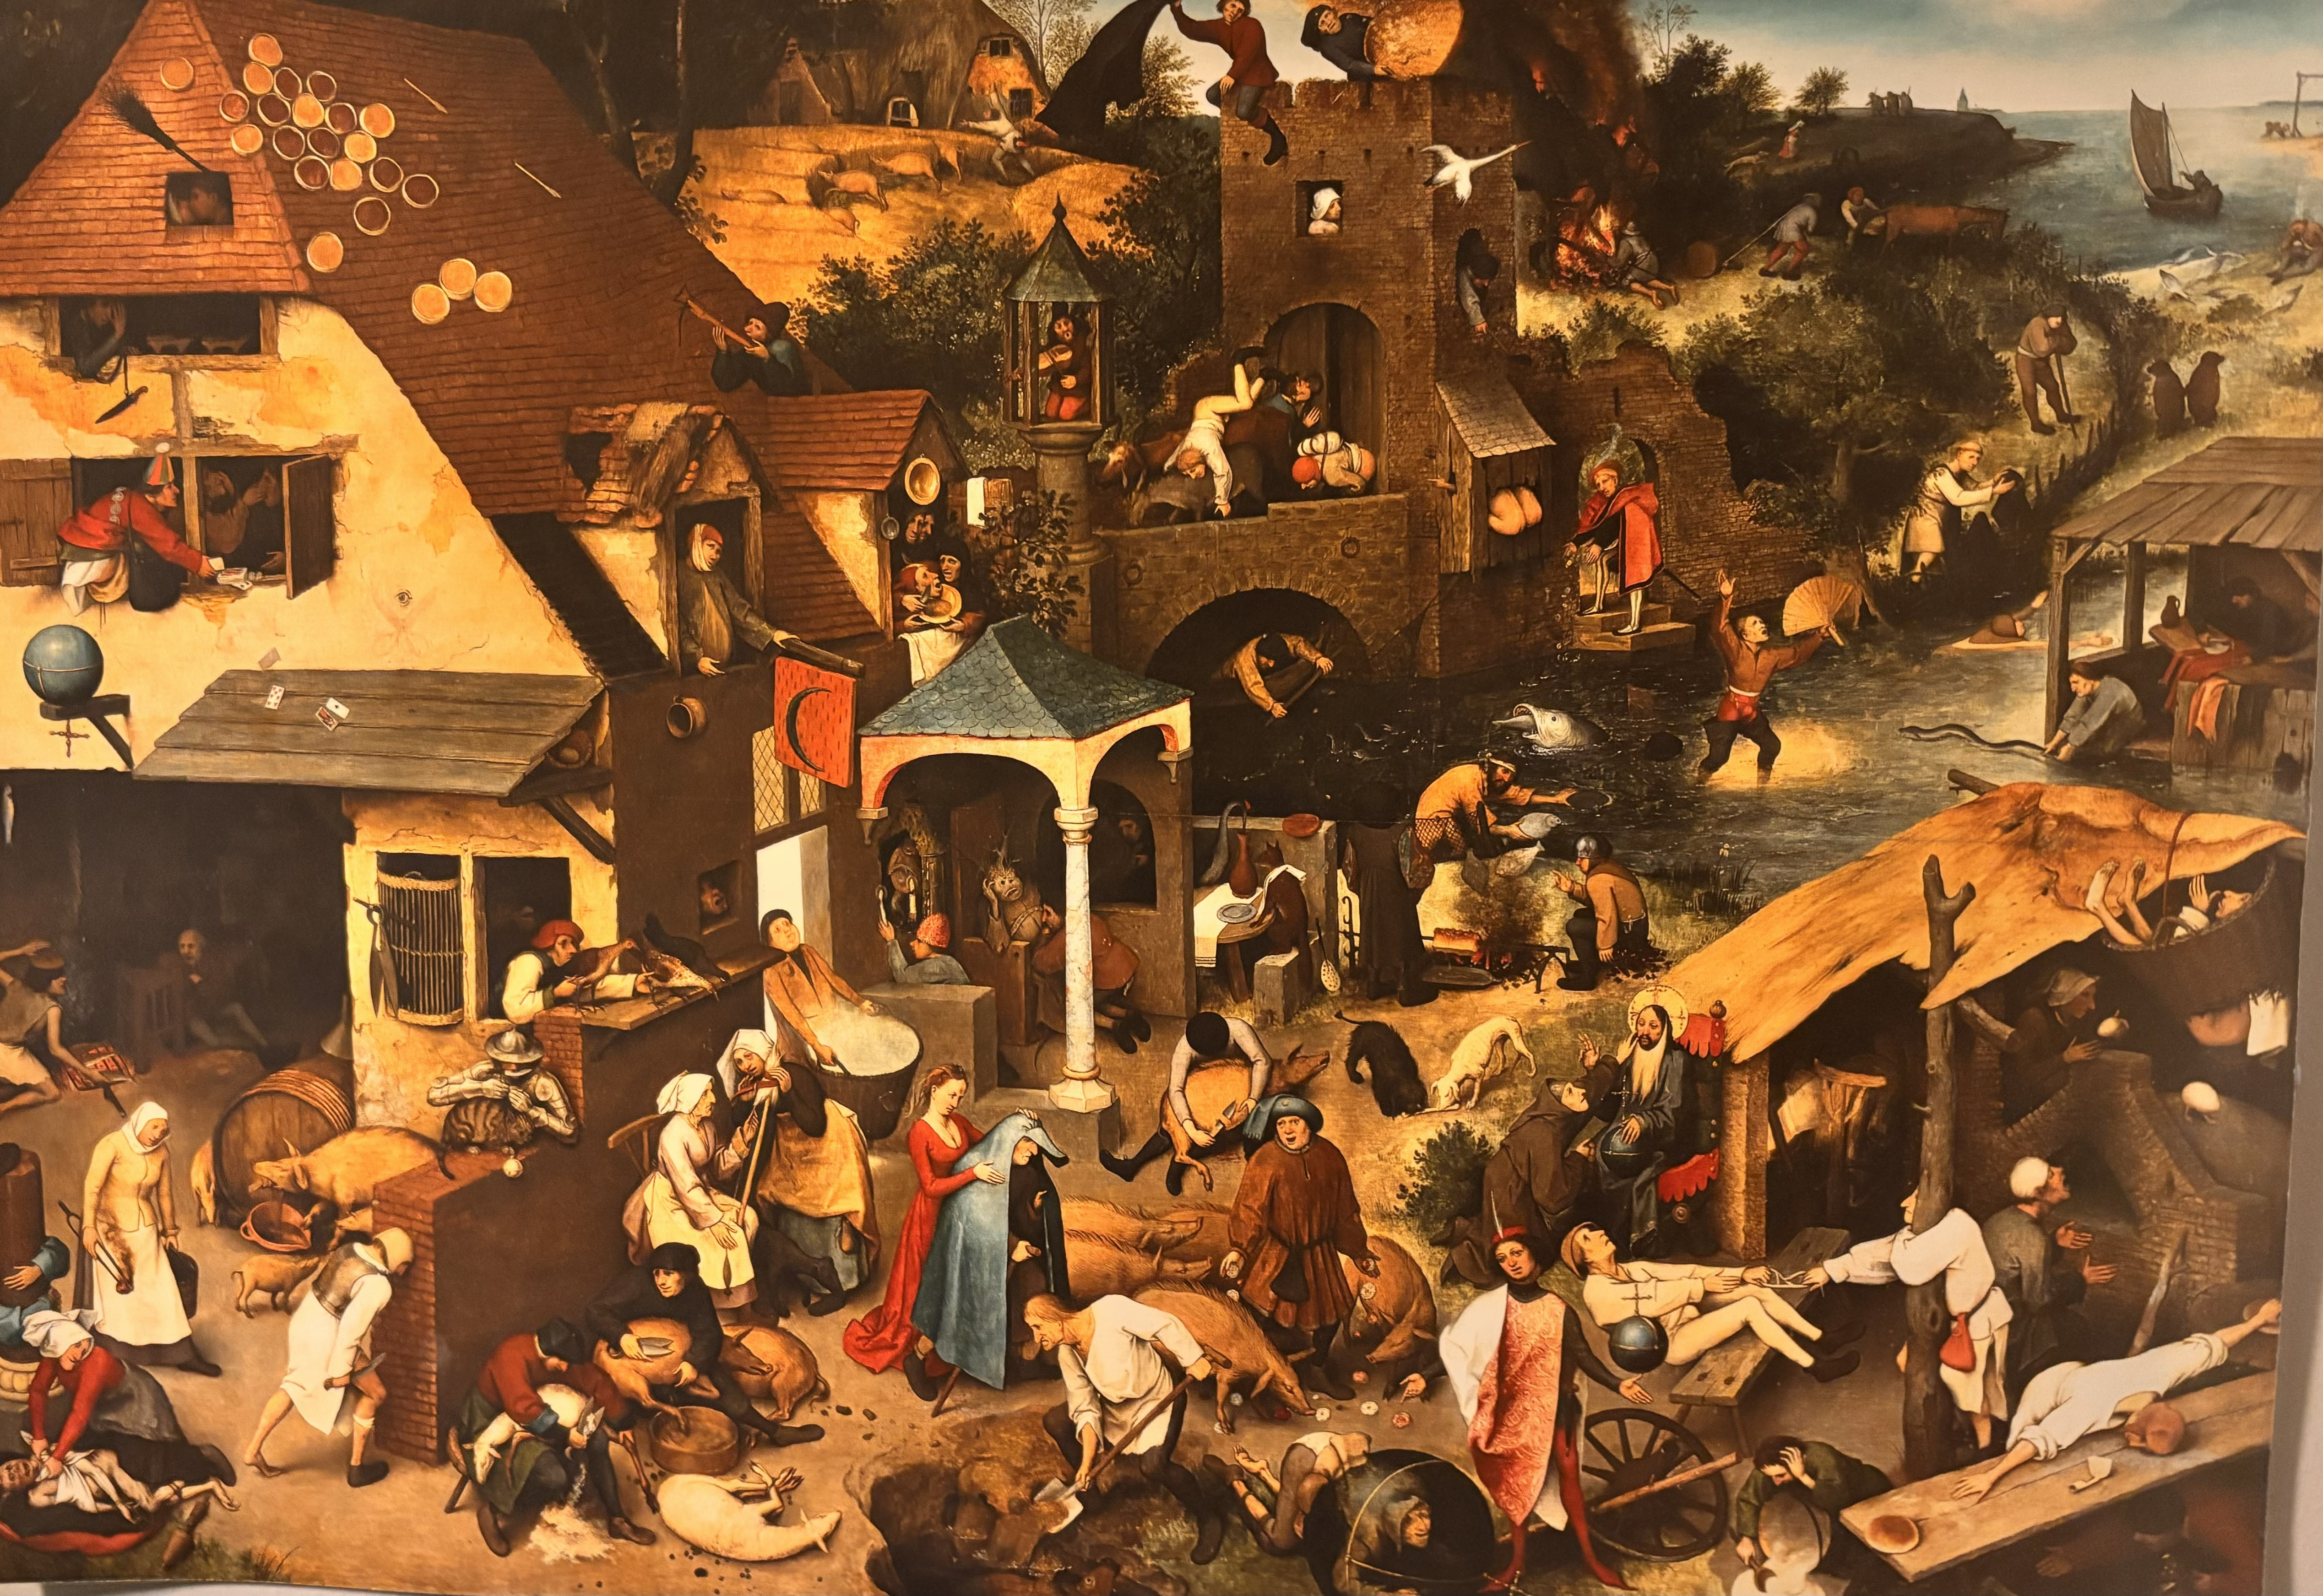
\includegraphics[width = \textwidth]{chapter8/IMG_ch8/proverbe} \caption{Pieter Bruegel’s Netherlandish Proverbs (oil on wood, painted 1559). For years, this painting has fascinated me. One of the reasons is that it was painted in a time still marred by plagues. Enough time had persisted since the first wave in 1345 for the societal upheaval to become fully manifest. Above all, it appears to depict a time in which the previous structures, customs, and societal norms are in complete disarray. A time of flux and dynamism, perhaps representative of what Nietzsche said in the quote referenced above: \ \noindent"At this turning-point of history there manifest themselves, side by side, and often mixed and entangled together, a magnificent, manifold, virgin-forest-like up-growth and up-striving, a kind of tropical tempo in the rivalry of growth, and an extraordinary decay and self-destruction, owing to the savagely opposing and seemingly exploding egoisms, which strive with one another 'for sun and light.'"} \label{redone} \end{figure}





\begin{figure}[H] 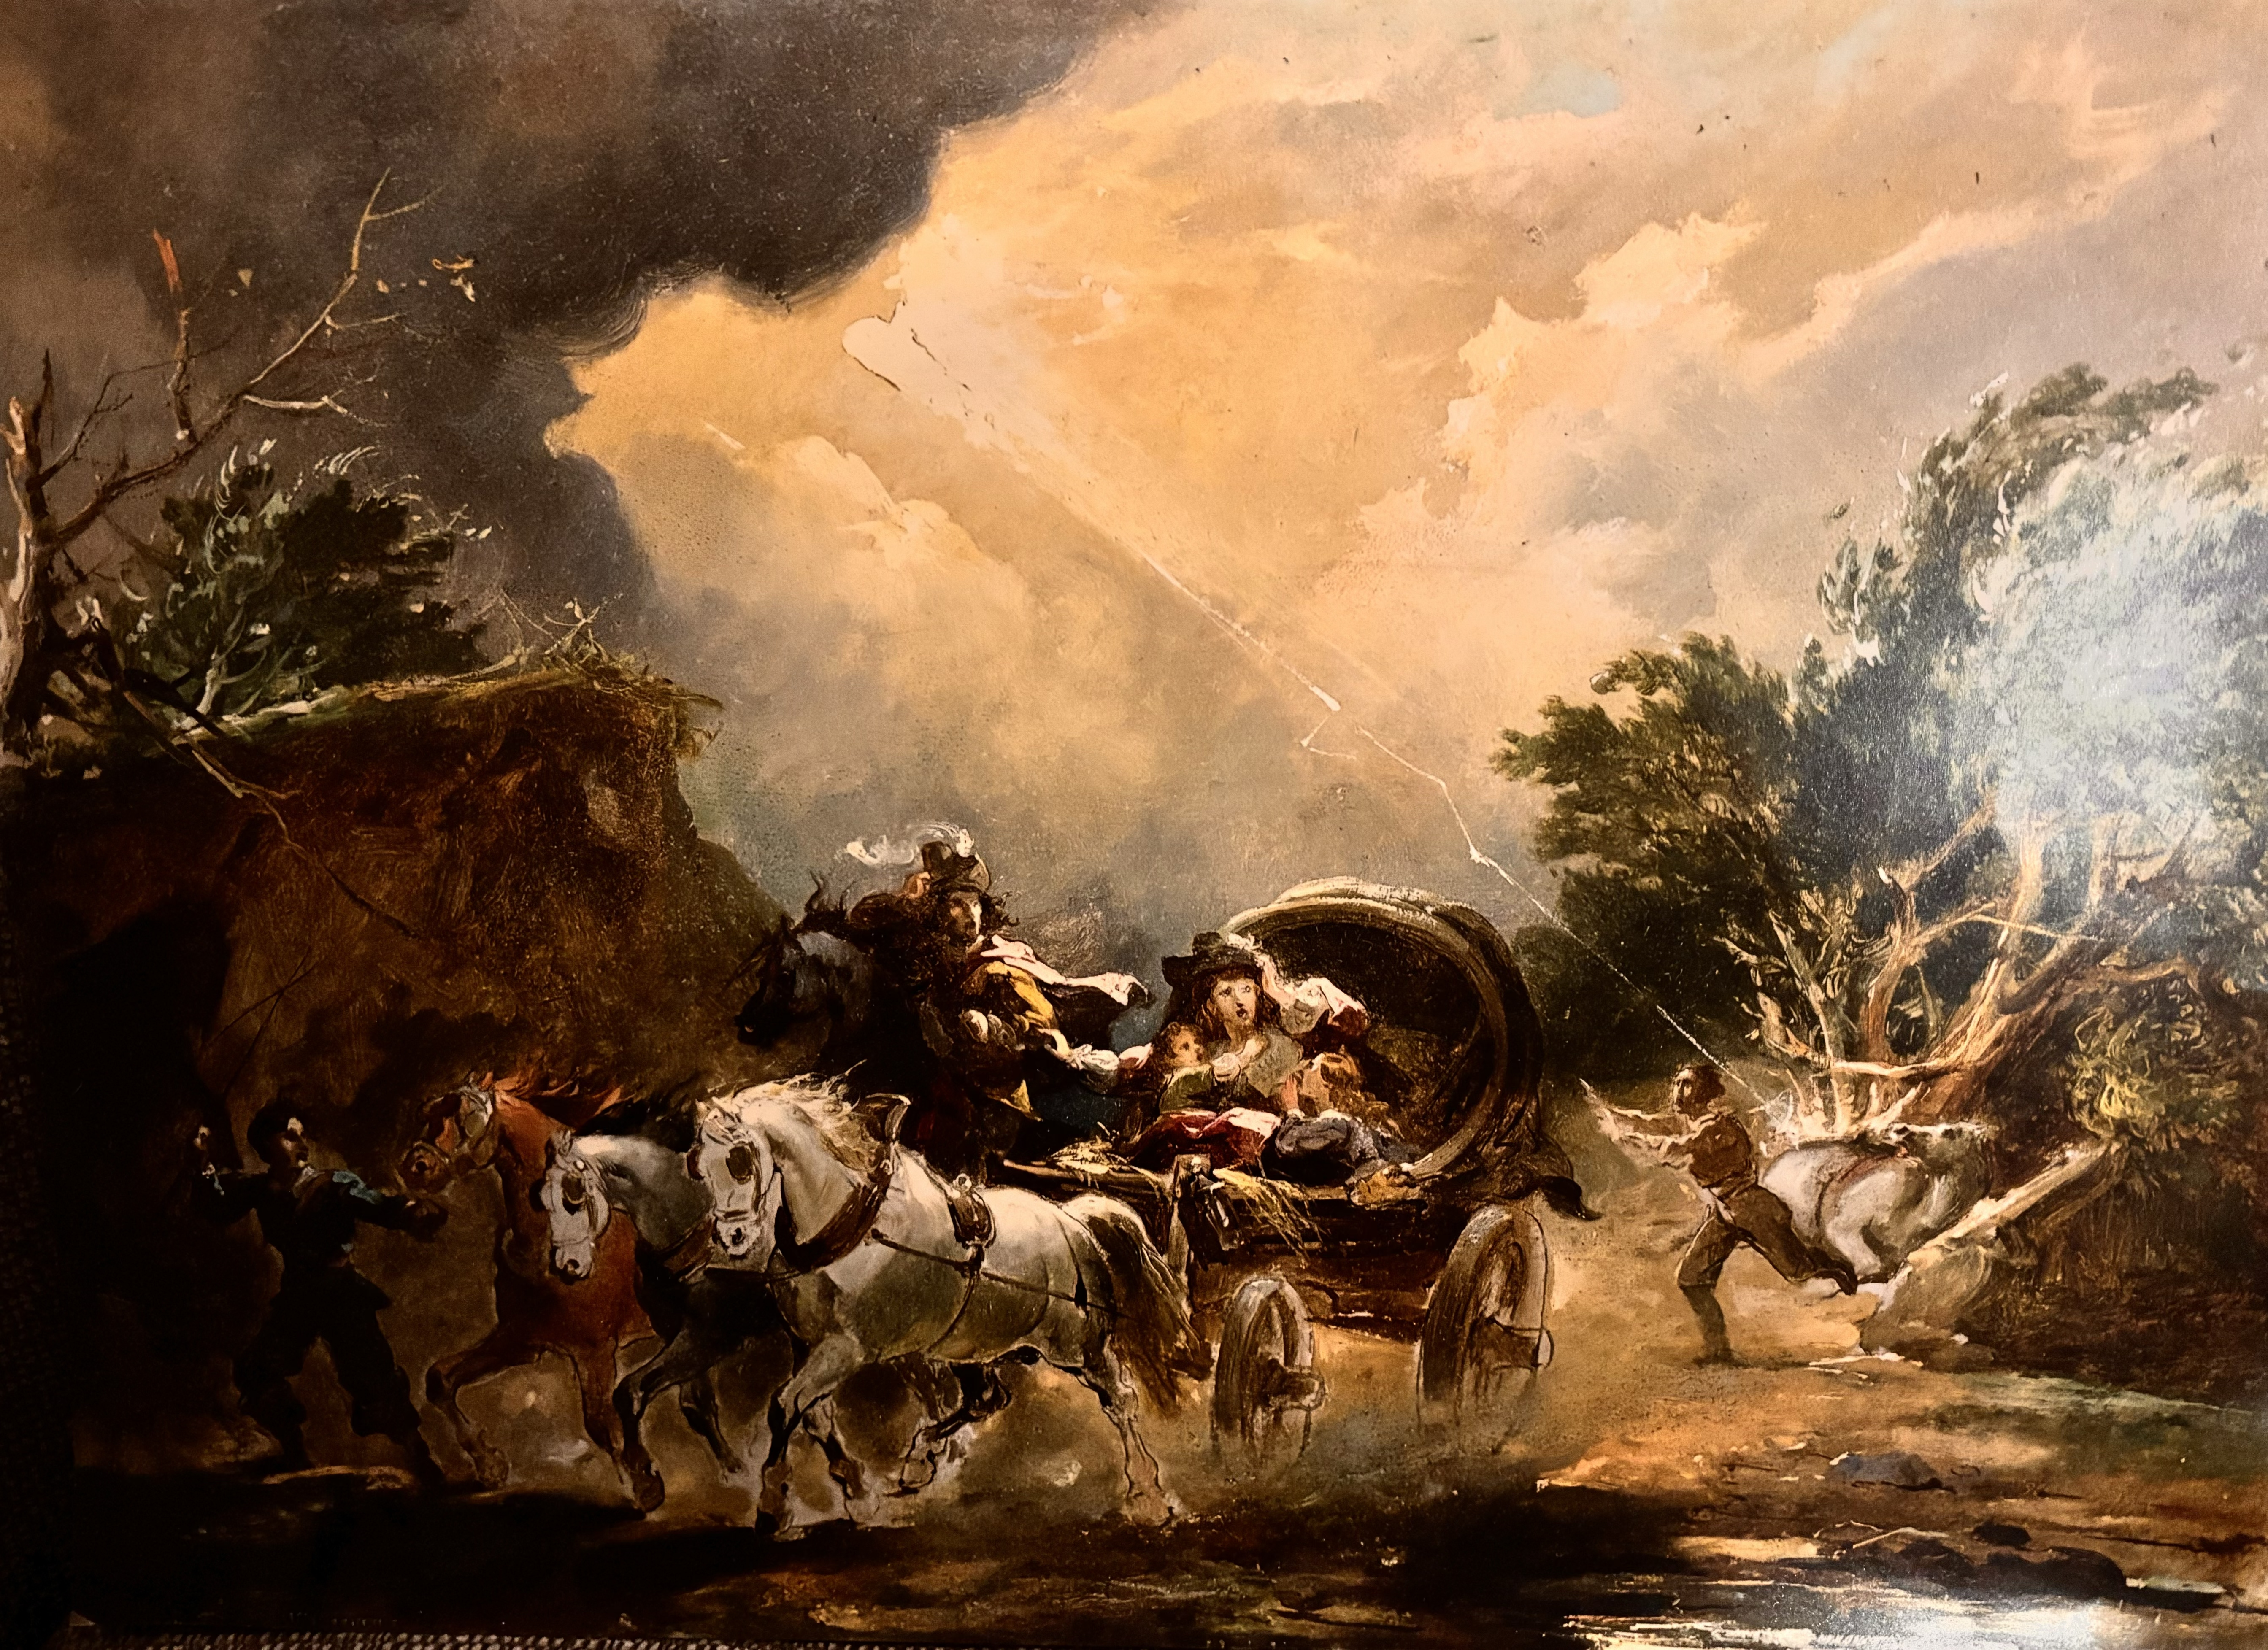
\includegraphics[width = \textwidth]{lightning}
\centering
\pagebreak \caption{Coach in a Thunderstorm (Philippe Jacques de Loutherbourg, 1790).  It almost appears as if the cart, the horse and the person are eminating from the lightning strike,  rather than merely running away from it after being struck on the road. As if the energy of the lightning itself is creating the activity we see before us.  We have no way of knowing whether Philippe Jacques intended for this this interpretation.  But the emergences of sudden complex order through immediate resolutions of large potential,  seems like it might be consistent with the situaten of  a country (France) at the verge of instability,  which ultimately manifested into full blown societal revolution only a few years later.  To be clear, I am suggesting the interpretation that the motion depected is an ephemeral dissipative structure,  momentarily created by the lightning. } \label{redone} \end{figure}








\section{Birth-plague model}

Birth
$$\pr{\Delta \xt = 1, \Delta \yt = 0} = \beta \xt \Delta t +o(\Delta t)$$
Corruption (instantiation of plague)
$$\pr{\Delta \xt = -1, \Delta \yt = 1} = \delta \xt \Delta t +o(\Delta t)$$
Infection (spreading of plague)
$$\pr{\Delta \xt = -1, \Delta \yt = 1} = \alpha \xt\yt \Delta t +o(\Delta t)$$
Dying (death of plague infected)
$$\pr{\Delta \xt = 0, \Delta \yt = -1} = \mu \yt \Delta t +o(\Delta t)$$
No event
$$\pr{\Delta \xt = \Delta \yt = 0} =1 - \lrbs{(\beta + \delta + \alpha \yt) \xt + \mu \yt} \Delta t +o(\Delta t)$$





\begin{figure}[h!]
    \centering
    % First row
    \begin{subfigure}{0.49\textwidth}
        \centering
        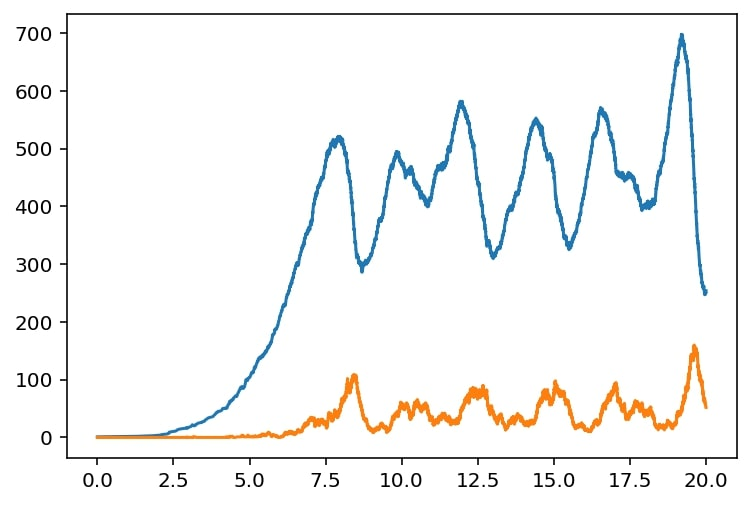
\includegraphics[width=\linewidth]{bpPLOT}
        \label{fig:figure1}
    \end{subfigure}
    \hfill
    \begin{subfigure}{0.49\textwidth}
        \centering
        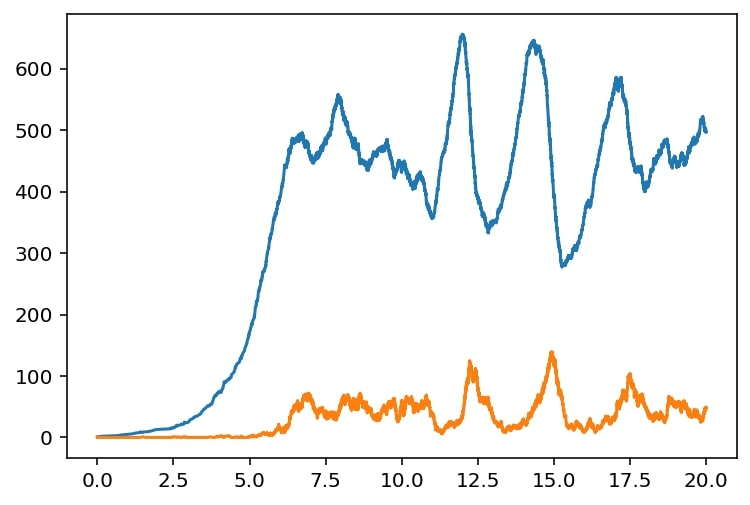
\includegraphics[width=\linewidth]{bpPLOT2}
        \label{fig:figure2}
    \end{subfigure}
    
    % Second row
    \vspace{0.5cm} % Optional: adds some space between rows
    \begin{subfigure}{0.49\textwidth}
        \centering
        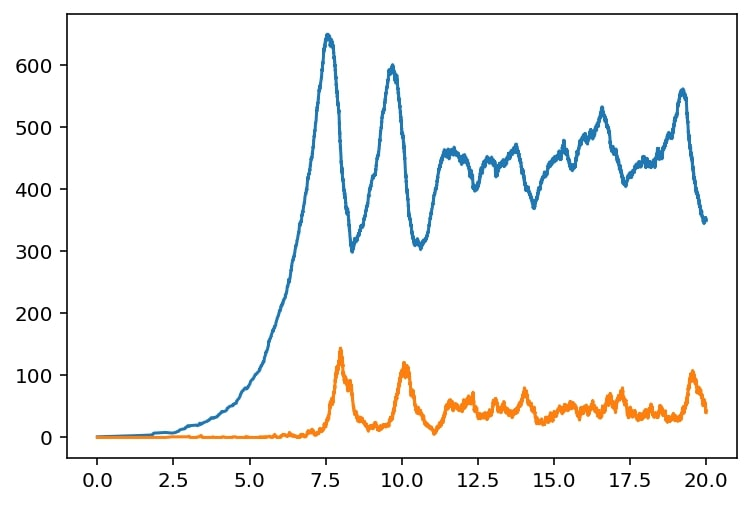
\includegraphics[width=\linewidth]{bpPLOT3}
        \label{fig:figure3}
    \end{subfigure}
    \hfill
    \begin{subfigure}{0.49\textwidth}
        \centering
        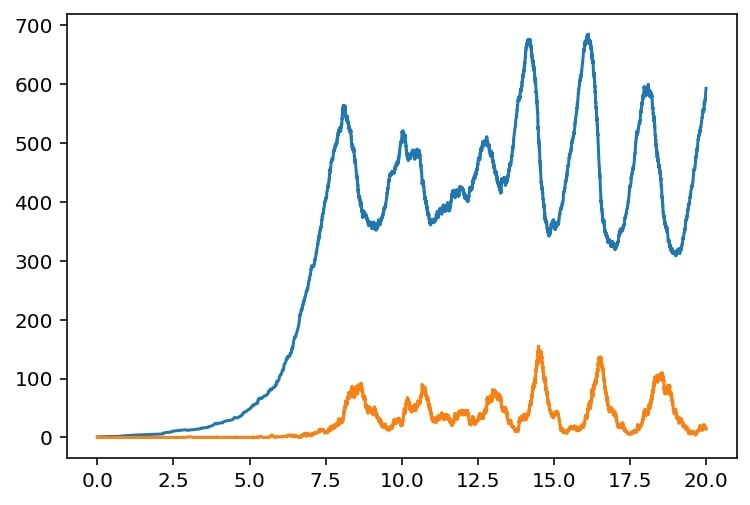
\includegraphics[width=\linewidth]{bpPLOT4}
        \label{fig:figure4}
    \end{subfigure}
    
    \caption{($\beta, \delta, \alpha, \mu$) = (birth, corruption, infection , dying) = (1, 0.1, 0.02, 10). Four realisations of the birth plague model. In each, the blue line is $\xt$ (population count), $\yt$ is the number of plague infected individuals.}
    \label{fig:four-figures}
\end{figure}




\section{(Density dependent) Vitallity birth-plague model}

To attempt to illustrate the cyclic phases of multiplicative bifurcation, waining, colapse, and re-sustaining development as seen in both turbulence shedding, and the rise and often suddern fall of living dissipative structures at multiple scales. \par 

\vspace{10pt}
This model is a combination of the previous two (birth-plague and RRRR).  It incorporates the idea from RRRR that catastrophe (but in this case plague instantiation) is driven by a situation of relative per capita scarcity (per capita reffering to the multiplicative agencies brought about by successive bifurcations).  This, general concept, in principle being at least artistically applicative to multiple phenomena,  but notably, the dissipative structures of fluid turbulence shedding and population collapse. 

This model is a combination of the previous two (birth-plague and RRRR). It incorporates the idea from RRRR that catastrophe (in this case, plague instantiation) is driven by a situation of relative per capita scarcity (per capita referring to the multiplicative agencies brought about by successive bifurcations). This general concept is, in principle, at least artistically applicable to multiple phenomena, but notably to the dissipative structures of fluid turbulence shedding and population collapse.

(Potential availability)
 $$\ddt{V} = \xi - p \xt$$
Birth
$$\pr{\Delta \xt = 1, \Delta \yt = 0} = \beta \xt \Delta t +o(\Delta t)$$
Corruption (instantiation of plague)
$$\pr{\Delta \xt = -1, \Delta \yt = 1} = \delta \xt \Delta t +o(\Delta t)$$
Infection (spreading of plague)
$$\pr{\Delta \xt = -1, \Delta \yt = 1} = \alpha \xt\yt \Delta t +o(\Delta t)$$
Dying (death of plague infected)
$$\pr{\Delta \xt = 0, \Delta \yt = -1} = \mu \yt \Delta t +o(\Delta t)$$
No event
$$\pr{\Delta \xt = \Delta \yt = 0} =1 - \lrbs{(\beta + \delta + \alpha \yt) \xt + \mu \yt} \Delta t +o(\Delta t)$$





\subsection*{Plague in popular culture}

\textbf{Roses poem:}\\

\begin{center}
"Ring-a-ring o’ roses\\
A pocket full of posies;\\
Atishoo, atishoo,\\
We all fall down."
\end{center}

\noindent
\textbf{Edgar Allen Poe -- The masque of the red death}
\begin{center}
\begin{quotation}
\noindent
``All these and security were within. Without was the “Red Death.” \cite{poe2020masque}\\

\noindent
\hfill \dots \hfill\\

\noindent
It was toward the close of the fifth or sixth month of his seclusion, and while the pestilence raged
most furiously abroad, that the Prince Prospero entertained his thousand friends at a masked ball of the
most unusual magnificence.
It was a voluptuous scene, that masquerade.\\

\noindent
\hfill \dots \hfill  \\

\noindent
And thus too, it happened, perhaps, that before
the last echoes of the last chime had utterly sunk into silence, there were many individuals in the crowd
who had found leisure to become aware of the presence of a masked figure which had arrested the
attention of no single individual before. And the rumor of this new presence having spread itself
whisperingly around, there arose at length from the whole company a buzz, or murmur, expressive of
disapprobation and surprise — then, finally, of terror, of horror, and of disgust.\\

\noindent
\hfill \dots \hfill \\

\noindent
And now was acknowledged the presence of the Red Death. He had come like a thief in the night.
And one by one dropped the revellers in the blood-bedewed halls of their revel, and died each in the
despairing posture of his fall. And the life of the ebony clock went out with that of the last of the gay.
And the flames of the tripods expired. And Darkness and Decay and the Red Death held illimitable
dominion over all."
\end{quotation}
\end{center}


%%%%%%%%%%%%%%%%%%%%%%%%%%%%%%%%%%%%%%%%%%%%%%%%%%%%%%%%%%%%555
























































\chapter{Conclusion -- Evolved strategy of Yersinia Pestis}












The main finding across all of the (see appendix B) above cases (specifically, where the total replicative ``rate-density'' remains fixed between comparrisons), both in the continuous time and discrete time cases, is that the mean of the process at the end of the specified period is identical.  How it gets there varies, along with what happens after. Also, the variance and distribution seems to vary.  But the point remains -- early replicative enphasis given constant overall "potential replicative density", gives no advantage over a specified period, to the expected overall growth. \ 
Of course, this assumption of eqivalent "replicative density" does not apply to the case of comparrison between complete etracellular growth when set against the alternative of an initial "replicative boost" in macrophages. 











\subsection*{Two common exceptions to this rule}

\subsubsection{Non-conservation}
Non-finite supply of replicative means. Basically when the key assumption is removed. Perhaps a higher replication rate is accessible at larger population sizes.



\subsubsection{Monopoly effect}
Matthew effect






In appendix B, there is a summary of some work witch mathematically demonstrates a property of branching. That articifially front weighted replicative advantage --- when assuming an overall constant "replicative potental" --- does not give any advantage to a process with regards to its expected growth. In more intuitive terms, say a bacterial population had access to a finite supply of food on an agar plate, if it was to use more of it towards the beginning, and less later, there would not be any advantage to its overall expected growth. This seems relatively obvious, but I just wanted to check, and the maths checks out. At least in the mean. When it comes to the variance and distribution of outcomes, there is some nuance,  but let us leave this aside. \par 

What of the case of plague finding early replicative in macrophages? The condition of constant "replicative potential" does not apply when comparing with the case of less fecund extracellular replication. 




\section{Two phase}



Thinking about the replication of Yersinia pestis within the body. There are two distinct phases in its pathogenesis. Namely, the preinflamatory and the postinflamatory periods.To recall,  in the first of these, YP replicates mostly intracellularly within macrophages. Then, as the body recognizes the alien presence and mounts a neutrophil attack, YP switches to extracellular replication. 

Due to the fact YP doesn't begin with extracellular replication, it seems sensible to assume that there is an advantage to living within macrophages. As a rudimentary model of this behavior, we can take in simple terms that the replication rate is higher in this proinflammatory phase. That viral multiplication is easier within the macrophage intracellular environment. 

In the cell there are fewer of the extracellular mechanisms of innate immunity: thinking specifically about complement and bacteriophages. 

Perhaps there is an adaption to the specific presentation of bacteriophages in a particular host on the time scale of YP infection dynamics. That is, within only a handful of replication cycles, small variations to the bacteria cause the population to gain resistance to these host-specific bacteriophages. 

Such a dynamic could be captured with a model using the two phases, but with a decaying death rate in the second extracellular phase
$\mu(t) = a + a\ee^{-t}$. If we were to take this process individually. That is with some initial count of replicators undergoing only this second phase. Given the decaying death rate, there may be an initial period in which replication is subcritical. And in this case, the size of the initial population would become vitally important to whether the infection persists.







\subsection{Host to host Galton Watson process}



Consider a host-to-host branching process in which the dynamics are a basic Galton-Watson process with probability $p$. But that $p$ is defined by a within-host dynamic. Essentially, if the infection within the host attains a threshold bacterial load, the infected person will infect two more people. If it does not and gets killed off by the immune system, no further infections will result from that individual. Thus, the replication probability, $p$, results from the chance of this happening; of the infection persisting and ascending to a high infectious load. \par

The simplest version of this would be a simple birth-death process and a defined threshold value.  We are then interested in the probability of the process ``hitting'' one threshold or the other (either the upper positive threshold, or 0), and this is the replication probability.\par

Then, we are in a position to compare different models. Especially, the two-phase models (with and without variable death rate). It will be straightforward to show that probability of ``host-to-host transmission''  (reaching the threshold) will be greatly altered by the inclusion of this initial phase. The time at the beginning when YP temporarily exploits the within macrophage environment to gain an early advantage. This early advantage being of vital importance to the outcome from the onset of the second phase. 






\subsection{Two phase PGF}

For reasons soon described, we are really only interested in the overall extinction probability, but this is the starting point. 


$$G^{(\text{whole-process})}(x,t)    = \begin{cases}
G^{(\text{phase-1})}(x,t), & t< t_c\\
\sum_{k=0}^\infty   \pr{\xx_{t_c}^{(\text{phase-1})} = k} \lrb{G^{(\text{phase-2})}(x,t-t_c)}^k, & t>t_c
\end{cases} 
$$


$$ \pr{\xx_{t_c}^{(\text{phase-1})} = k}   =  \lrb{k!}^{-1}  G^{(phase-1)}_{kx}(0, t_c)$$




There are two phases. The second is a birth death process that is only slightly supercritical, $\beta > \mu$ but $\beta \approx \mu$. The first is a BDC process for which $\lambda >> \mu$ (favours replication). The first phase represents the intracellular phase of an infection, second, the extracellular phase.\par

Consider the situation of an infected individual. Assume they will either go on to infect two more individuals, or they will recover and the infection will die with them. In this way, a Galton Watson style epedemic takes place. Suppose the former case takes place with probability $p$. Then, the expected number of infections caused is $2p$. Now, whether the person infects others will depend on the success of the infection within them.\par

In a birth death process, which the within-person infection can crudely be modelled as, if the process is supercritical, it will either blow up, or die out. Ceasing eventually with some probability, $p_0$. Lets say that the person goes on to infect in the case that the infection does not cease (blows up in the simplified BD model), happening with probability ($1-p_0$). In this way $p = 1-p_0$.\par

So take the second phase outcome as the deciding factor. The probability that the infection in the second phase wont cease will depend on what happens in the first phase. That being a BDC process, we can compute $p_0$ of the second phase with the following formula (law of total probability)

$$p^{\text{whole-process}}_0 = \sum^{\infty}_{k=0} \pr{\mathcal{K} = k} \lrb{p_0^{(\text{phase-2})}}^k$$ 

$$p_0 = b + \sum^{\infty}_{k=1} \frac{\delta}{\lambda} \lrb{\frac{1}{a}}^{k} \lrb{\frac{\nu}{\beta}}^k$$ 


$(\nu/\beta)^N$ being the probability of eventual extinction of a standard BD. Note, the first phase BDC uses $\lambda$, $\mu$ and birth/death rates; the second phase BD process uses $\beta$, $\nu$. The $b$ term comes in at the $k=0$ case (probability of death in first phase BDC). \par
Hence, the probability of infecting another two people is $p = 1-p_0$. And the $R_0$ number of this Galton-Watson epidemic is

$$ \mean{Z} = 2p = 2\lrb{1 -  b + \sum^{\infty}_{k=1} \frac{\delta}{\lambda} \lrb{\frac{1}{a}}^{k} \lrb{\frac{\nu}{\beta}}^k} $$


The question is, how does this value depend on the dynamics of the first phase. On the expected burst size and time, these depending substantially on the catastrophe rate, $\delta$. 


The above formula is for the BDC to birth death case.  One of a few choices of model:

\begin{itemize}
\item BD - BD
first BD higher effective replication ratio (goes on for some defined time)
\item BDC - BD
BDC higher replication rate (goes on for time dictated by cat rate)
\item Const - BD
\item Const - BD (subducive) To represent the host bacteriophage adaption hypothesis. 
\end{itemize}

\noindent


\begin{figure}[H]
    \centering
    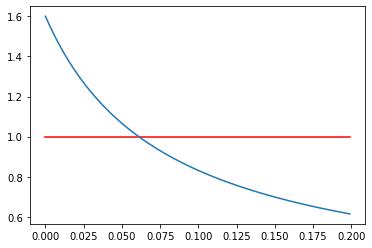
\includegraphics[width=0.5\textwidth]{chapter9/IMG_ch9/rough.png} % Adjust the width as needed
    \caption{ $(\lambda, \mu) = (1, 0.2)$ in the first phase, and $(\beta, \nu) = (1, 0.9)$. This is the host-to-host GW proliferability measure ($\mean{Z}$) in the BDC to BD case. The plot shows $\mean{Z}$ plotted against $\delta$. What is shown is that for supercritical epidemic spread (under the given assumptions), the initial phase of infection in macrophages should produce a sufficient bacterial load to overcome the likelihood of extinction in only near-supercritical growth in the extracellular phase. This is a consequence of $\delta$ being sufficiently small. That is, the propensity for the macrophage to burst being low permits a higher expected release in this crucial initial phase.}
\end{figure}



\begin{figure}[H]
    \centering
    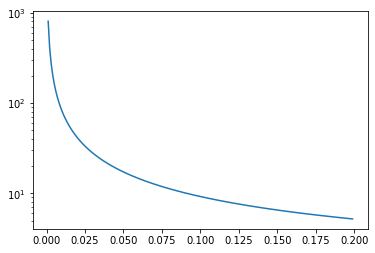
\includegraphics[width=0.45\textwidth]{chapter9/IMG_ch9/rough2.png}   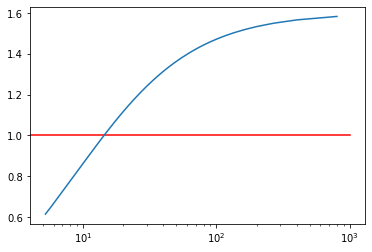
\includegraphics[width=0.45\textwidth]{chapter9/IMG_ch9/rough3.png} % Adjust the width as needed
    \caption{Left: mean burst size as a function of catastrophe rate $\delta$.  Lower propensity to burst, higher burst size.
Right: GW epidemic replication number $\mean Z$ plotted against mean burst size. High burst size, greater chance of the infection surviving the minimally supercritical pro-inflammatory phase, higher probability of not going extinct, and thus growing exponentially, causing host-to-host proliferation.}
\end{figure}








\section{Quadrant argument}





To begin  understanding YP's particular invasion strategy, we can start by painting a schematic picture of the circumstances it comes up against in the body. For some reason YP has evolved to at first grow intracellularly, then transition to primary extracellular replication. Let us simplify
 the case of intracellular replication to being within either macrophages or neutrophils only (ignoring for simplicity the presence of dendritic cells, eosinophils, basophils and mast cells. Though these are no doubt also relevant in reality). We can make the simple assumption that the within-neutrophil environment is more hostile to YP than that of Macrophages. 

Macrophages are the run of the mill, generalist leukocyte whereas neutrophils are more specialist killers. As I understand it, it is mainly neutrophils that are recruited and released on mass in response to recognition of such a bacterial infection as YP.  

If we took YP replication to be a simple BD process, this assumption would be reflected in the death rate within neutrophils being higher than that within macrophages. There is the complication discussed previously where killing within leukocytes has something to do with granules (neutrophils
 have more of these). This producing the aforementioned non-autonomous effects. But here, it seems sufficient to gloss over this underlying reality to take the death rate as merely fixed. 

So $\mu_N > \mu_M$. What about $\mu_E$, the extracellular death rate. I want to put forward the supposition that this is somewhere in between the two. That the situation outside of cells is relatively more hostile than within macrophages, and relatively less than within neutrophils. 
The argument for this assumption is that if there was no advantage to being within macrophages, it seems unlikely that YP would have evolved to exploit their intracellular environment at all. And, if there was an advantage to being within neutrophils (over the extracellular environment), it begs the question why phagocytosis would
 be resisted when a swarm of these hosts presents itself. Hence, let us proceed with the assumption 
$$\mu_N > \mu_E > \mu_M$$

with each of the three environments exhibiting standard birth-death dynamics with equal birth rate,
$$\beta_N = \beta _E = \beta_M.$$
This itself is an assumption that begs some justification. There may be variation among these replication rates; in reality, differing supply of nutrients and energy within cells may cause faster generational production. But for the present argument, it seems best to take them as equal so as not to introduce unnecessary complication. And anyway, the distinction of key importance is the overall effective replication rates, $\beta_i - \mu_i$. 


\vspace{10pt}
\hrule
\vspace{10pt}

\noindent
\textbf{Aside:}  There are other explanations for why YP might initially favour macrophage absorption. Especially, the possibility that macrophages are merely used as a transport mechanism for YP to get to the Lymph nodes which probably have a greater supply of food.\par
It is also possible that the initial pro-phagocytosis phase is a lingering hangover from the time the bacteria lives within a flea. 
For now, we will ignore these genuine possibilities to explore the argument that there might be a more fundamental strategic advantage. 

\vspace{10pt}
\hrule
\vspace{10pt}

\noindent
Following pathogen recognition, the body recruits neutrophils and delivers them to the site of infection. In a simplified framework, we can model this by there being a stepwise increase in neutrophils at a defined time, $t_N$, following the onset of infection. In reality, the fact that YP ``hides'' within macrophages could act to delay the onset of neutrophils. This would manifest in our model at $t_N$ changing according to the bacteria choice of strategy. But this detail can be ignored for the present argument, because whether it is advantageous for YP to be absorbed or not does not here depend on the time at which the neutrophils arrive. 


The bacteria to gain the best proliferative advantage will need to maximise its effective replication rate, $\beta_i - \mu_i$. Its evolutionary process has been able to select for whether to accept or resist phagocytosis at stages of the infection, but we will take it that the bacteria can not discriminate between absorption by macrophages and neutrophils. 


Because  $\mu_N > \mu_E > \mu_M$ and $\beta_N = \beta _E = \beta_M$, it follows that
$$\beta_M -  \mu_M > \beta_E -  \mu_E >  \beta_N - \mu_N.$$
Macrophages offer the best replicative opportunity. But because we assume YP can not differentiate between macrophages and neurtophils, the expected replicative rate for each strategy will depend on the probability that absorption is executed by a macrophage over a neutrophil. In the case of a pro-phagocytosis strategy, let us take the probability of macrophage absorption as $p_M$; $p_N$ for neutrophils. If we also assume that one of these outcomes is certain, it follows that $p_M = 1 - p_N$. These probabilities resulting from the ratio between neutrophils and macrophages present, 
$$p_M = \frac{\# M}{ \#N + \#M}, \quad p_N = \frac{\# N}{ \#N + \#M}.$$
with $p_N$ increasing at time $t_N$. \par
The mean effective replication rates for each strategy will hence be as follows:

\begin{itemize}
\item \textbf{Pro-phagocytosis}: $R_{\text{pro}} = p_M(\beta_M -  \mu_M) + p_N (\beta_N - \mu_N)$
\item \textbf{Anti-phagocytosis}: $ R_{\text{anti}}  = \beta_E -  \mu_E $ 
\end{itemize}
And with some rearrangement, the former becomes
$$ R_{\text{pro}} =(1-p_N)(\beta_M -  \mu_M) + p_N (\beta_N - \mu_N)$$
$$R_{\text{pro}} =p_N \lrbs{ (\beta_N - \mu_N)  - (\beta_M -  \mu_M)}  +     (\beta_M -  \mu_M).$$

\noindent
Pro-phagocytosis will cease to be a favourable strategy when 

$$R_{\text{anti}} > R_{\text{pro}}$$ 

\noindent
which occurs when the proportion of neutrophils, $p_N$, increases beyond a threshold: 

$$p_N > \frac{ (\beta_M -  \mu_M)  -  (\beta_E -  \mu_E) }{   (\beta_N - \mu_N)    -   (\beta_M -  \mu_M) } .$$

\noindent
Noting that $\beta_N = \beta _E = \beta_M$, this becomes

$$p_N > \frac{  \mu_E - \mu_M }{    \mu_M - \mu_N} .$$

\noindent
Given this threshold is crossed with the onset of the neutrophil influx at time $t_N$, an argument would be satisfied for why YP has evolved to switch between the two strategies. 

 




\section{Public good accumulation --- a model,  and potential relevance to Y. pestis}

Matt Asker, Lluis Hernandez and Mauro Mobilia work in the field of antimicrobial resistance \cite{asker2023coexistence}.    Cancerous cells exhibit two varieties: those resistant to a drug, and those succeptible. The resistant ones produce a substnce which they expell into their surrouning matrix. It's called a public good because it facillitates the resistance of all cancer cells to the drug, both the resistant and suceptible types. \par 
It occured to me that there may be something similar going on with Y. pestis in macrophages. -- This is purely my speculation, and may not at all be the case, but even if it isn't, the dynamics may be interesting in and of themselves.  -- Y. pestis has evolved resistance to the toxins that are presented within macrophages.  It occured to me that if Y. pestis were to execute this resistance using a "public good" substance,  that it would be confined within the resident macrophage and thus concentrated, rather than being dispersed.  Something like this could further support the argument that the within-macrophage environment provides a replicative advanage (assuming there are also toxins and other challenge factors (possibly bacteriophages) in the extracellular space). 


\begin{figure}[H]
    \centering
   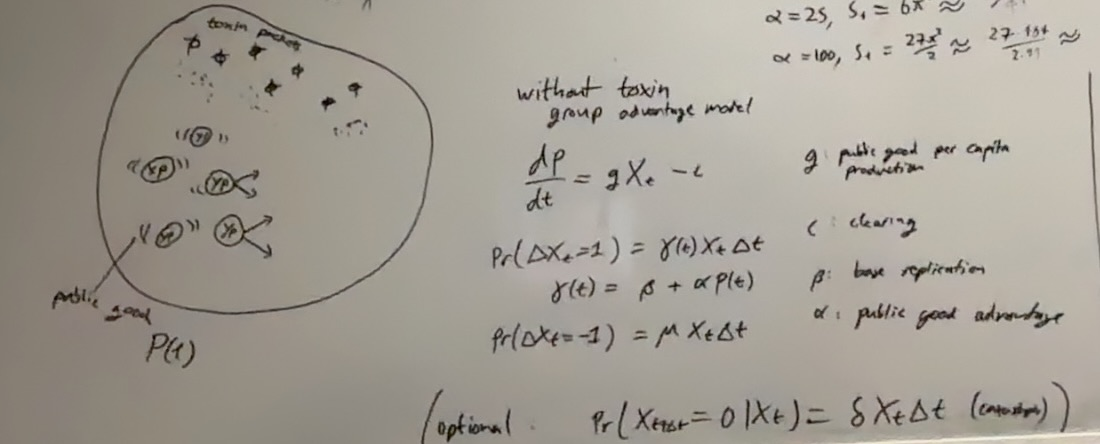
\includegraphics[width=0.99\textwidth]{chapter9/board.jpeg} % Adjust the width as needed
    \caption{Y.  pestis represented within a macrophage along with toxin containing packets.  Public good, $P(t)$ is produced by }
\end{figure}


\subsection*{Model for public good replication without directly accounting for toxic granules}

The effect of the toxic immune substance can be incorporated into the linear death rate.  Of course, this overlooks the dynamics of toxin depletion as discussed in chapter 6,  but it seems good in the interest of simplicity.  And the point of focus is the dynamics of this public good.  Let us make the simplified assumption that the presence of the "public good" increases the replication rate ($P(t)$: public good concentration; $\xt$: Y. pestis bacteria): 


$$\ddt{P} = g \xt - c,$$
$$\pr{\Delta \xt = 1} = \gamma(t)\xt\Delta t + o(\Delta t),$$
$$\gamma(t) = \beta + \alpha P(t),$$
$$\pr{\Delta \xt = -1} = \mu \xt \Delta t.$$

\begin{itemize}
\item[$g$:] public good production rate
\item[$c$:] public good clearing rate
\item[$\beta$:] base birth rate
\item[$\alpha$:] public good advantage
\end{itemize}
It might well make more sense for the presence of public good to reduce the death rate rather than increase the birth rate.  Another formulation could be thought up along these lines. \par 

\subsection*{Potential quantity of interest}

Suppose we consider a successive version of this process for which in the case of late time non-extinction it is assumed that the infected cell dies and infects two more cells.  A simplification which creates a sort of Galton Watson process in which the division probability is subject to embedded dynamics.\par 
In this case,  for the overall GW process to be supercritical,  the probability of within-cell non-extinction must be greater than one half.  We could as the question of what would be the minimum required incident cohort size into a cell to achieve this,  especially in the case where $\mu > \beta$, in which the public good plays a critical role.  In other words, 

$$\text{inf}\{K : \lim_{t\to\infty}\lrb{\pr{\xt > 0 | \xx_0 = K }}\} = \text{?}$$
This could be computed numerically. 


\subsection*{Notes -- public good in a closed group}

What if there is some replication advantage to a cohort of Y. pestis bacteria living within the enclosure of a macrophage; and what if there is something like a public good produced by the bacteria, and confined within the boundary of the host cellular membrane -- this underpinning a benefit of within group (macrophage) cooperative co-existence. \par 

\vspace{10pt}
\noindent
Something that comes to mind is,  as in other cases of cultural practice,  in Jewish communities it has historically been virtuous to cooperate within the community whilst facing outwards with more competitiveness.  In Shakespeare's "The merchant of venice" it is revealed that at the time (16h CE) it was forbidden for Jews to lend money with interest within the community,  whilst being acceptable to do so with Christians. \par

\vspace{10pt}
\noindent
Just like the individual is rewarded -- paid by gains of cooperative advantage - for being effective to the purpose and success of the private group; so the private group can be rewarded for benefiting circles of wider scope.\par 
And going in the other direction, the individual within the individual is crucial in its avarice when chasing personal enterprise. \par 
Surely these things don't need to be contradictory. 



%My feeling is that somewhere in all this is a helathy middle ground between the two extremes of a particular ideological spectrum.  Crudely,  that between the socialist and the individualistic libertarian capitalist.  On the one hand we have everyone driven to povery by the abolition of accute progress; on the other hand, we have the pathology of extreme inequality.  Something in the middle might see a framework of nested groups internally cooperating and externally competing. 



















































































































%%%%%%%%%%%%%%%%%%%%%%%%%%%%%%%%%%%%%%%%%%%%%%%%%%%%%%%%%%%%%%%%%%%%%%%%%%%%%%%%%%%%%%%%%%




















%%%%%%%%%%%%%%%%%%%%%%%%%%%%%%%%%%%%%%%%%%%%%%%%%%%%%%%%%%%%%%%%%%%%%%%%%%%%%%%%%%%%%%%%%%





\appendix









\chapter{}


\section{Punctuated equilibria — Gould may have got it right,  but maybe  the Vajrayana schools beat him to it}


Change is a consistent fact of life.

But change does not occur gradually or constantly; it churns at times, more vivaciously than others.

At these times — relative bursts of undetermined chaotic manifestation — the future gets decided by a long series of happenstances, each of which might seem inconsequential at the time. Together, they draw out an arc through tremendous divergences of possibilities: both into the future worlds of better circumstances, but also, and more largely, down into less favorable ones.

Periods of relative dynamic stasis are interspersed by upheavals of varying magnitude with unpredictable consequences. Like earthquakes, they release built-up tension that gets triggered by some alignment of forces that were ready to give way \cite{bak1991self}.

I feel it is this property of punctuated unfolding through time that Padmasambhava may have been onto when he wrote the Bardo Thodol. Bardos are transitory phases through which passage can lead to a number of varying eventualities. The idea is something like: the sum total of what “you” (and perhaps those with you) have “done” — your karma — will, in theory, influence your passage through the transition.

There are also bardos of becoming in evolutionary processes. At certain (relatively short) periods in history, there has been great flux, more substantial than the background average.

\section{Brief overview of the main Buddhist schools}

For reference, Vajrayana translates crudely to “the way of the lightning bolt.” Of Theravada (Hinayana — lesser vehicle), Mahayana (greater vehicle), and Vajrayana, Vajrayana Buddhist practices supposedly offer the fastest route to enlightenment. Theravada (Hinayana) is the orthodox school, which still follows the Pali Canon. It is still practiced in Sri Lanka, and much of Southeast Asia, especially Myanmar, Thailand, Laos, and Cambodia. Critics of Theravada Buddhism refer to it as Hinayana (the lesser vehicle) because there is an emphasis on prioritizing the enlightenment of a few selected monks. These monks strive after nibbāna, while leaving everyone else, as it were, below.

The early Mahayanists seemed to have addressed the social problems this creates by inventing the Bodhisattva — an ideal individual who, upon attaining the condition of Arahant (completely free of all defilements relating to craving and attachment), purposefully delays their enlightenment in order to help others on their way to the cessation of dukkha (suffering). This is why Mahayana gets its name as the great vehicle: because the ideal is to make everyone enlightened, rather than just a few monks.

It almost seems like a funny coincidence that the cultural trends in countries following Buddhism share patterns depending on whether they follow Theravada or Mahayana. Case in point: the country where Zen Mahayana Buddhism formed, China, became communist (for the many). In contrast, in Thailand, a country of Theravada Buddhism, there is still a firm monarchy; and there have been a number of scandals in which monasteries have illegally accumulated huge stores of wealth in the form of gold and cash. In Sri Lanka (Theravada), the president recently had to flee his residence in a helicopter to escape angry crowds of violent protestors.

My feeling is that there is a dissipative story to be told about the organizational hierarchy of these monastic traditions. It’s almost as if something is being accumulated in the inner circles of the monasteries, and that this quality is being distributed. The Mahayanists even have a word for it — Bodhicitta (Heart awakening).

Gurdjieff referred to "Hydrogens" (a substance of the person which can be accumulated and refined). These hydrogens are a form of energy which can be used to overcome the influences of emotive draws from the environment.

\section{Major scale shifts through evolution in geological time}

The emergence of cities following the agricultural revolution might be seen as one of only a few great scale shifts that have taken place to life across geological time.

Prokaryotes got together to make eukaryotes.
Eukaryotes got together to make multicellular algae.
Simple multicellular organisms combined to form the Cambrian multi-organ fauna.
Then, after a great expanse of time, swarming insects tried it first — but we did it better.
Mammals teamed up to create companies and institutions, which themselves can be seen as living, breathing supra-organisms.
Like the discs of Ediacran fauna emerging on the sea floor, London and Paris compete for various nutrients in the local matrix.

\subsection{Grouping-up --- a dissipative structural emergence?}

There appears to be this general phenomenon where, in order to become competitive, individual agencies have teamed up to form cooperative groups. Together, these groups have been able to outdo the competition, ultimately taking a lion’s share of the available food and persisting.

In dissipative structure theory, the degree to which a formation of local order (negentropy) is possible depends on the energy flux taking place. Higher flux means more potential for a greater complexity of emergent order, with more ordered structures generally being more dissipative (capable of dissipating at a higher rate).

The scale-jump phenomenon mentioned above seems to align with this. When multiple individual agencies come together to form a coherent entity, that entity will almost by definition be an object of higher organizational complexity. But surely to kick-start such a process, there needs to be some excess of potential energy flux to be taken advantage of. Perhaps this jump to a higher dissipative throughput itself requires a sort of “kick” in the form of relatively excessive energy availability to create the space for active competition in which the "group" strategy could emerge.

At this point, we are faced with the question of what was happening at the time of each of these major scale jumps listed above. There is some speculation that at the time of the emergence of eukaryotes, there was an excess of oxygen present in the atmosphere and seas. Then something similar may have been the case with the Cambrian explosion. There is also some theory relating to a huge Ice Age (mass extinction) which took place shortly before. In the case of the KT mass extinction, the radiation of mammals took place in the presence of relative food abundance and the lack of predators after the dinosaurs died out.

Then there is the case of the emergence of towns and cities. Agriculture provided the means of producing an excess of food, which could be bought and sold in exchange for goods, services, and eventually currency. This freeing up of dissipative potential, it seems, paved the way for the vast increases in the complexity of human group behavior which followed.

Before you know it, with all these people congregating in one place, living in close quarters with livestock and poor sanitation, the potential was created for the infestation of parasitic agencies. Rats, fleas, and pathogens found their way in and replicated freely in the excess of their new host-to-host dominion. It is thought that it was in this period (circa 3000 BCE) that Yersinia pseudotuberculosis, an enteric (gastrointestinal) pathogen, evolved into Yersinia pestis, an agent spread both by fleas and by the transfer of infected air (miasma) from lung to lung in primary pneumonic plague.

\section{Arupa $=$ Formless}

From the space of forms to matters of the formless, the spiritual jump takes place when we suspect that there are agencies alive which do not have physical form. They live suspended in a network of minds.

But of course they do exist:

Viruses (memes) of the mind are easy to identify, and they fall right across the spectrum from the destructive to the benign, beneficial, or even revered. The best are found preserved in the unadulterated religious traditions of old. (Let’s study the Pali Canon?)

But the question is, how complicated can these life-ethereal forms of the formless truly be? Yes, it seems we have viruses, but what about bacteria? Eukaryotes? Multicellular algae?

And where do Krishna, Ram, and Hanuman fit into all of this? Not to mention St. Peter,  Mary,  Muhammad and Jesus.\\

\noindent
On a smaller scale, it seems that personalities can play out this kind of role. Individuals with a compelling history in a social group — when they leave or when they die, they do not completely die. Because people remember them, and their mannerisms persist. Their acts are reenacted, knowingly or unknowingly, by a series of individuals. Maybe sometimes primary reincarnations (people who end up filling their role in the group). In this way, a funeral may be a sort of coming to life, to a greater or lesser extent.


In the Pali Canon, there are described the 8 jhānas or meditative absorptions—states in which you are completely absorbed in the meditative experience. These range in a spectrum from the four rūpa jhānas (rūpa—of form) to the 4 arūpa jhānas, from the crude to the refined; from the domain of physical sensations to the realms of transcendent rapture.

Incidentally, the root word of jhāna (chan, which originally comes from the Sanskrit dhyāna,  also happens to be the root word for Zen, the Mahāyāna root school which emerged in China when crossbred with Taoism, before becoming Sōtō Zen in Japan.

In the Gurdjieffian theory, there is a hierarchy of worlds of influence. Lower worlds, where everyday people live, are influenced by successively higher worlds in the hierarchy of the "ray of creation." 


%The higher worlds, beyond those on Earth inhabited by the ruling classes, supposedly are inhabited by deities of ordered significance. This is consistent with the metaphysics of the Bhagavad Gītā, in which there are a series of realms above the terrestrial world of birth, death, and rebirth. It says that, given piety in this life, one may be reborn into one of the higher (as it were, extraterrestrial) realms. The individual ātman may return, but if they do fall back through the stratosphere (according to the Gītā), they will be reborn into a pious, sage-like, or aristocratic family.

%I can't help but wonder if, after the decline of Christianity, we in England foolishly replaced transcendent religious idealism with mundane notions of class and social status linked erroneously with material possession. Whether this is true or not, the interesting point is: What is the true currency of this old transcendent religious idealism? I have some ideas, but it's time to pack this up and hand in the thesis.

\subsection*{Scene from the film "Meeting with remarkable men"}

It's a film about the early years of the 20th centuary mystic and philosopher,  George Ivanovitch Gurdjieff.  When working as a tour guide to make ends meet, he encounteres a Russian Prince, Yuri Lubovedsky.  Together, they continue work to explore the religious traditions of old seeking answers,  and more importantly,  questions.    

Lines quoted from a scene of the biographical film about Gurdjieff --- Meeting with Remarkable Men ---:\\

\begin{itemize}
\item[\textbf{G.}] Since I was a child, I has a feeling that something...  something is missing in me.  I felt that apart from my ordinary life, there is another life, a life which is calling me.  I had to be open to it. This question never gives me any peace, and I've become like a hungry dog, chasing everywhere for months.  


\item[\textbf{Y.}] You should be happy you've had that experience. When I was your age,  I was only interested in myself. \par I was always concerened with satisfying my needs,  and those of my family.  Suddenly, my wife died in childbirth. I could not recover from the shock. \par 
Life had no meaning anymore.  One day, an old dervish came to the house and asked for me.  We talked together for a long time. And as he spoke,  \textbf{I experienced something far greater than all the impulses I normally obeyed. } When the dervish left me, the experience vanished. But I knew what I was looking for; for that, help was needed.  Fortunately, I had the means to travel.  I went to Africa, India, Afghanistan and Persia. I organised special expeditions to places where I thought I might find an answer.  I lived in monestaries, and met many people with interests similar to my own. 

\item[\textbf{G.}] How can I meet such people? I need to know...


\item[\textbf{Y.}] What do you need to know? 


\item[\textbf{G.}] I want to learn; I want to understand. 


\item[\textbf{Y.}] Be careful, what do you call learning?\par 
If it means storing up experiences and beliefs, it will tie you like a cord and prevent you from knowing.  \textbf{Knowing happens directly. Where not even a thought stands between you and the thing you know. }\par 
Then you see yourself as you are, not as you would like to be.  I have learned how difficult this can be. \par
Dear young friend, I will do everything I can to help you attain your aim. 




\end{itemize}


\noindent


























\chapter{}





\section{Birth death front weighted replication bias}

Chances of persistence beyond an early development is made more likely with special conditions during the outset. 

In life as in nature, there are many cases in which favorable circumstances are arranged for in initial growth period. In the case of seeds contained in fruit, and embryogenesis in nutrient-packed eggs, a store of energy is supplied for the offspring to grow up to a minimally functional form. In this way, they have an improved chance against the myriad stochastic challenges of life beyond the nest.

The so-called ``Allee effect'' illustrates the dynamic in which a population requires a minimum census to persist and grow. For example, when a population of wild fish are harvested to a sufficiently small population, factors such as the lacking saftey in numbers effect may lead to their premature extinction. 

A similar notion of development beyond a sort of critical mass can be observed in the adoption of technologies, infrastructure and even ideas. A fine example is the fax machine. Subject to what has been termed an anti-rivalrous effect, whereby the product value increases as more people buy them; for faxing to make sense, a sufficient percentage of your friends need to be contactable.


A monopoly effect can give a company or a species the advantage required to persist in the hustle and bustle of an early-stage innovative period. Without this, successive players may continually eliminate one another.

Though eventually until by natural circumstance, a handful win out and succed to a majority standing. Even witout a direct fittness advantage, such is the consequence of the Matthew effect where between competing agencies, small fluctuations are aplified until smaller groups get pushed aside. 

A curious exception counteraction to this effect can be seen in the case of rainforest insect populations. An infective fungus (cordyceps) attacks all species indiscriminately, and because of mere statistiacal obligation, the more populase species is affected more often. Thus takes hold a sort of anti incumbancy effect where species are punished for growing to large. It is though that this effect leads to a greater diversity among insects in the region as more species are able to coexist without being out competed by a monopoly.

Aside: even basic computer simulations of this effect yield the result.  

Figure + details in caption. 




Coming back to the initial topic of interest. this imortance of an initial advantage. How fundamental is it? What if we strip back such numerous complexities as safety in numbers, like with the allee effect? Take for example a humble branching process, only, with a slight twist.

Consider basic Galton Watson branching over just 10 generations. Starting with one initial replicator, at each time step, all present units either divide wp $p$ or die wp $1-p$; each leaving behind either 2 or 0 copies. Say for example $p=0.6$. The process is supercritical and so $\mean{Z_n}$ will increase multiplicatively by generation. Specifically, 
$$\mean{Z_n} = \mean{Z_{n-1} }\mean{Z_1} = \mean{Z_1}^n$$.
But consider the fate of that initial unit. It will die \%40 of the time, putting an end to the lineage before it gets started. Now consider a slightly modifed version of the simple model. For the 10 generations, let there be 10 distinct replication probabilities, $p_i$, for $i = 1,\dots,10$, but conditioned on some total alloted number of percentage points. That is, 
$$\sum_{i=0}^{10} p_i = 10p$$
where $p$ is from the previous case. In that case, $p=0.6$, so the total must amount to $10\times 0.6 = 6$. But these probabilities can be arranged arbitrarily. The question is: will there be some advantage to the process if replication is, as it were, front loaded, so that the first few rounds of replication hold better odds of persistence than later ones. It would seem that in this way, ``dead off the starting blocks'' made less likely; this leading to a superior expected progression by round 10...  Right?\par 
As it happens, the expected dynamic appers to be unchanged regardless of how $p_i$ are chosen. 


%DISCRETE TIME P_i EZ




Moving on the the cont time version. 


\begin{align*}
     \pr{\Delta\xx= 1} &=  \beta(t)\xt \Delta t,  &&\text{(birth)}\\
      \pr{\Delta\xx= -1} &= \mu \xt\Delta t,  &&\text{(death)}\\
     \pr{\Delta\xx= 0} &= 1 -  \lrb{  \mu + \beta(t)}\xt\Delta t,  &&\text{(no event)}
\end{align*} 



We will explore three different version of the model. $\beta(t)$ will be the only difference between them:

\begin{itemize}
\item $\beta_1(t) = a \ee^{-t}$,
\item $\beta_2(t) = b + a \ee^{-t}$, with special attention to the $b=1$ case
\item $\beta_3(t) = \begin{cases}
\lambda_1 &  t< t_c\\
\lambda_2 & t > t_c
\end{cases}
$  with $\lambda_1 > \lambda_2$ and some switching time, $t_c$
\end{itemize}


This is all to explore the effect of a front weighting to the replication rate. Where in the early phase of observed dynamics there is a disproportionalely higher replication rate. In the first two cases, we see what happens to the mean and the distribution when the overall ``rate density'' for a given period is identical to a case in which the rates are constant.

\subsection{Exponential decline to 0 ($\beta_1(t) = a\ee^{-t}$)}


Here, we specifically set $\mu = 1$ and $\beta(t) = a \ee^{-t}$ for some constant, $a$.

We can set some future time, $T$ and compare two birth death processes: the one above, and a simple birth death process with linear rates. Crucially, the area under the curves, $\beta(t)$ should be identical when taken between 0 and $T$. This could be thought to represent some total food availabilty that a bacterial population has access to. With each unit of time, $\Delta t$, the replicators have access to $\Delta t \times \beta(t)$ units of the nutrient substance (this being read in the limit $\Delta t \to 0$).  In other words, we require that
$$T\beta_{\text{standard}} = \int_0^T \beta_{\text{variable}}(t) \dd t = \int^T_0 a \ee^{-t}\dd t = a\lrb{1 - \ee^T}.$$ 
So 
$$a = \frac{\beta T }{1 - \ee^{-T}}.$$
We might also want to impose that the process is supercritical, but this condition may be relaxed.\par 
To construct a full picture of 

So how will early-time weighted replication affect the overall process dynamics? To construct a full picture, it will be of assistance to obtain the mean, variance and extinction probability. Fortunately, these can all be obtained using the probability generating function.\par
We have examples above using the method of characteristics to solve a PDE for the generating function. There may be only one type in this case as opposed to two, but here we have a replication rate which varies with time, and this does complicate the analysis. The PDE for pgf, $G(x,t)$, is very similar to as in the absorption-birth-death case and can be retrived simply by ignoring the second type and setting the absorption rate $\alpha$ to 0:

 $$\pddt{G} = \lrb{\mu - (\mu+ \beta(t))x + \beta(t) x^2}\pdd{G}{x}$$

Here we are exclusively treating the variable-rate case. The simple birth-death process is sufficiently well covered to where we can take the required formulas from a text book (linda allen). $\mu$ is set to 1 to allow for analytic tractability, but with scaling of $a$ and $T$, this poses no real restriction to the investigation. Hence, we seek to solve,

 $$\pddt{G} = \lrb{1 - (1+ a \ee^{-t})x +  a \ee^{-t}x^2}\pdd{G}{x}$$
 Following the standard procedure, we begin by re-parametrizing $(x,t)$ to $(s,\tau)$,
 
 Then, by looking for solutions on characteristic lines of constant $s$ we find the the characteristic ODEs: 
\begin{align}
\dda{G}{\tau} &= 0\\
\dda{t}{\tau} &= -1\\
\dda{x}{\tau} &= 1-(1+a\ee^{-t})x + a\ee^{-t} x^2
\end{align}
We must also decide on initial conditions for the characteristic lines:
$$x(s, \tau = 0) = s, \qquad  t(s, \tau) = 0.$$
Similar to previous cases, the first two characteristic equations yield
Like in the previous section the first two characteristic equations yield: 
$$G(s,\tau) = \phi(s),$$
and ultimately,
\begin{equation}
G(s,r,\tau) = s^N.
\end{equation}
And,
$$t = -\tau.$$   
Then, we turn to the final characteristic equtation,
$$\dda{x}{\tau} = 1-(1+a\ee^{\tau})x + a\ee^{\tau} x^2.$$
(notice the switch from $t$ to $-\tau$). The solution is given by

But with $\tau = -t$ the actual equation is 
 $$\dda{x}{\tau} = 1-(1+a\ee^{\tau})x + a\ee^{\tau} x^2.$$
 which has solution

$$x(\tau) = \frac{\ee^{a\ee^\tau - \tau}}{ - a\text{Ei}(a\ee^\tau) + \text{Const}}$$
or
$$x(t) = \frac{\ee^{a\ee^{-t} + t}}{ - a\text{Ei}(a\ee^{-t}) + \text{Const}}$$
where 
$$\text{Ei}(z) =  \int^z_{-\infty} \frac{\ee^u}{u}\dd u.$$
is the so called exponential integral function. 

using $x(0) = s$

$$\text{Const} = \frac{\ee^a}{s -1} + a \text{Ei}(a)$$ 

$$x(t) = 1 + \frac{\ee^{a \ee^{-t} + t }}{  \frac{\ee^a}{s-1}  + a\lrbs{\text{Ei}(a) - \text{Ei}(a\ee^{-t})   }  }$$

Then, given $G_N(x,t) = s^N$,


$$G_1(x,t) = 1 + \frac{\ee^a}{  \frac{\ee^{a \ee^{-t} + t }}{x - 1}  +     a\lrbs{   \text{Ei}(a\ee^{-t})  - \text{Ei}(a)  }       }$$







\subsubsection{Mean}


We can get the mean using,

$$\mean{\xt} = \partial_x G(x,t)\large |_{x=1}$$


Writing 

$$G_1(x,t) = 1 +       \ee^a \lrb{b (x-1)^{-1}  + c}^{-1}$$

where $b(t) = \ee^{a \ee^{-t} + t } $ and $c(t) =  a\lrbs{   \text{Ei}(a\ee^{-t})  - \text{Ei}(a)  }   $

It follows that 

$$\partial_x G(x,t) = \frac{b\ee^a}{  \lrb{b + c (x-1)  } ^2}$$

Hence,

$$\mean{\xt} = \partial_x G(x,t) \large|_{x=1} = \ee^a b^{-1} = \ee^a \ee^{-a\ee^{-t}  - t}$$



We can also calculate the mean in another way. By considering its change over a small interval of time, one can easilly derive the following equation
$$\ddt{\mean{\xt}} = (\beta(t) - \mu)\mean{\xt} = \lrb{a\ee^{-t} - \mu} \mean{\xt}$$
This can be solved without difficulty to show that 

$$\mean{\xt}  = \ee^a \ee^{-a\ee^{-t}  - t}$$

Snap! Prior to further verification, this provides moderate confidence that the PGF is correct. 




\subsubsection{Variance}


The variance can be found using the PGF in the following way

$$\text{Var}(\xt) = \partial_{xx} G(x,t)\large|_{x=1} + \partial_{x} G(x,t)\large|_{x=1}  - \lrbs{ \partial_{x} G(x,t)\large|_{x=1}}^2$$

$$\text{Var}(\xt) = G_{xx}(1,t) + G_x(1,t) - \lrbs{G_x(1,t)}^2$$


The second derivative comes out as 

$$G_{xx} =  -2b\ee^a\lrb{b + c(x-1)}^{-3} c$$

then

$$G_{xx} (1,t) = -2\ee^a \frac{ c}{b^2}    = -2 \ee^a\frac{ {a\lrbs{   \text{Ei}(a\ee^{-t})  - \text{Ei}(a)  }} }{ \ee^{2a \ee^{-t} + 2t }} $$

so 

$$\text{Var}(\xt) =   -2 \ee^a\frac{ {a\lrbs{   \text{Ei}(a\ee^{-t})  - \text{Ei}(a)  }} }{ \ee^{2a \ee^{-t} + 2t }}     +    \ee^a \ee^{-a\ee^{-t}  - t}    - \lrbs{\ee^a \ee^{-a\ee^{-t}  - t}}^2 $$








\subsubsection{Full distribution}



We can construct the full distribution of state-probabilities, $\pr{\xt = k} = p_k$, using 

$$p_n   =   \frac{1}{n!} \frac{\partial^n G}{\partial x^n }\bigg|_{x=0}$$


For our case

$$G_{xx} =  -2b\ee^a\lrb{b + c(x-1)}^{-3} c$$
$$G_{3x} =  3!b\ee^a\lrb{b + c(x-1)}^{-4} c^2$$
$$G_{4x} =  -4!b\ee^a\lrb{b + c(x-1)}^{-5} c^3$$
$$G_{5x} =  5!b\ee^a\lrb{b + c(x-1)}^{-6} c^4$$

Theres a pattern 

$$G_{nx}  = (-1)^{n+1} n!\ee^a b( b + c(x-1))^{-(n+1)} c^{n-1}$$

Then 


$$p_n   =   \frac{1}{n!} \frac{\partial^n G}{\partial x^n }\bigg|_{x=0} =  \ee^a b( c - b)^{-(n+1)} c^{n-1}$$

(a $(-1)^{-(n+1)}$ multiple was taken out of the main bracket to cancel the front coefficient factor $(-1)^{n+1}$)



$$p_n   =  \frac{ \ee^a \ee^{a \ee^{-t} + t } }{   \lrb{a\lrbs{   \text{Ei}(a\ee^{-t})  - \text{Ei}(a)  }      -    \ee^{a \ee^{-t} + t }}^{n+1}   }   \lrb{ a\lrbs{   \text{Ei}(a\ee^{-t})  - \text{Ei}(a)  }  }^{n-1}$$


 $b(t) = \ee^{a \ee^{-t} + t } $ and $c(t) =  a\lrbs{   \text{Ei}(a\ee^{-t})  - \text{Ei}(a)  }   $
 
 
 (For $n\geq 2$)
 
 
 $$p_0 = G(0,t) = $$



\subsubsection{Comparisons}













\subsection{Exponential decline to 1 ($\beta_1(t) = 1 +  a\ee^{-t}$)}

With this slight modification, 
$$\beta(t) = l + a\ee^{-t},$$
(with $l = 1$ used for tractability) the fixed ``rate density'' condition becomes

$$a = \frac{(\beta_0 - l)T}{1-\ee^{-T}}$$


$$\dda{x}{\tau} = 1 - \lrb{1 + 1+ \ee^\tau} x + \lrb{1 + a\ee^{\tau}} x^2$$

$$x(\tau) = 1 + \frac{\ee^{a\ee^\tau}}{  \text{Const}  - \ee^{a\ee^{\tau}}  - \text{Ei}(a\ee^\tau)  }$$

with $x(0) = s$ and $G(x,t) = s$

$$G(x,t)  = 1 + \frac{\ee^a}{     \frac{\ee^{a \ee^{-t}}}{x-1}     +  \ee^{a \ee^{-t}} - \ee^a + \text{Ei}(a\ee^{-t})    - \text{Ei}(a)      } $$


Note

$$G(x,t) = 1 + \ee^a(b(x-1)^{-1} + c)^{-1}$$

with $b(t) = \ee^{a\ee^{-t}}$ and $c(t) = \ee^{a \ee^{-t}} - \ee^a + \text{Ei}(a\ee^{-t})    - \text{Ei}(a)  $

So using the multi-use identity, we can easily produce iterative $x$ derivatives. 




\subsubsection{Mean}


Like in the previous section, the two methods of obtaining the mean yield the same formula. Both the pgf and the basic ODE of $\ddt{\mean{\xt}}$ produce

$$\mean{\xt} = \ee^{a\lrb{1 - \ee^{-t}}}.$$


If instead of using the simplified form, we extend the birth rate to include a variable level, $l$,
$$\beta(t) = l + a\ee^{-t},$$
the mean becomes,

$$\mean{\xt} = \ee^{a\lrb{1 - \ee^{-t}} + (l - \mu)t}.$$

The simplified form ($\beta(t) = 1 + a\ee^t$) because it makes the pgf tractable. But this formula is slightly unsatisfactory. Ideally, we want in the late time limit that the process is slightly supercritical. My interest was to compare two processes which are both supercritical to see if the extra kick at the start (whilst maintaining fixed ``rate density'' in an interval) might advantage the process in the long run of its ongoing supercritical progression in comparrison to the standard linear alternative. As it happens, as we can see in the mean curve plots, this does not happen with the expected values.  




\subsubsection{Variance}



Using the identity in the appendix, for the $l=\mu=1$ case, we can find the variance in the following way. 

with $b(t) = \ee^{a\ee^{-t}}$ and $c(t) = \ee^{a \ee^{-t}} - \ee^a + \text{Ei}(a\ee^{-t})    - \text{Ei}(a)  $, 

$$G_x =  \ee^a b\lrb{b+c(x-1)}^{-2}, \qquad G_x(1,t) = \ee^a b\lrb{b}^{-2}  = \frac{\ee^a}{b}$$

$$G_{xx} =  -2 \ee^a bc\lrb{b+c(x-1)}^{-3}, \qquad G_{xx}(1, t) =  -2 \frac{ \ee^a  c}{b^2}$$

so 
$$\text{Var}(\xt) = G_{xx}(1,t) + G_{x}(1,t) - \lrbs{G_x(1,t)}^2$$

\begin{multline}
\text{Var}(\xt) = \frac{\ee^a}{b}  -2 \frac{ \ee^a  c}{b^2} - \lrbs{ \frac{\ee^a}{b}}^2 = \frac{\ee^a\lrb{b - 2c + \ee^a}}{b^2} = \\ \frac{\ee^a\lrb{ \ee^a +  \ee^{a\ee^{-t}} - 2\lrbs{   \ee^{a \ee^{-t}} - \ee^a + \text{Ei}(a\ee^{-t})    - \text{Ei}(a)    } }}{\ee^{2a\ee^{-t}}} 
\end{multline}




\subsubsection{Full distribution}


We can use the identity that if 

$$f(x) = (b(x-1)^{-1}  + c)^{-1}$$ 

then



$$\frac{\dd^n f}{\dd t^n}   =  n!b(c(1-x) - b )^{-(n+1)} c^{n-1} $$
 (for $n\geq 2$)
 to show that with 
 
$$G(x,t) = 1 + \ee^a(b(x-1)^{-1} + c)^{-1}$$

where $b(t) = \ee^{a\ee^{-t}}$ and $c(t) = \ee^{a \ee^{-t}} - \ee^a + \text{Ei}(a\ee^{-t})    - \text{Ei}(a)  $


$$G_{nx}(x, t) =  \ee^a n!b(c(1-x) - b )^{-(n+1)} c^{n-1}$$

and

\begin{align}
\pr{\xt = n} &=  \ee^a b(c - b )^{-(n+1)} c^{n-1} \\
&=    \ee^{(1+a)\ee^{-t}}\lrb{\text{Ei}\lrb{a\ee^{-t}} - \ee^a   }^{-(n+1)} \lrbs{\ee^{a \ee^{-t}} - \ee^a + \text{Ei}(a\ee^{-t})  }^{n-1}
\end{align}





\subsubsection{Comparisons}







The main finding across all of the above cases (specifically, where the total replicative ``rate-density'' remains fixed between comparrisons), both in the continuous time and discrete time cases, is that the mean of the process at the end of the specified period is identical.  How it gets there varies, along with what happens after. Also, the variance and distribution seems to vary.  But the point remains -- early replicative enphasis given constant overall "potential replicative density", gives no advantage over a specified period, to the expected overall growth. \ 
Of course, this assumption of eqivalent "replicative density" does not apply to the case of comparrison between complete etracellular growth when set against the alternative of an initial "replicative boost" in macrophages. 




\begin{figure}[h] % 'h' places the image near the current location
    \centering % Centers the image
    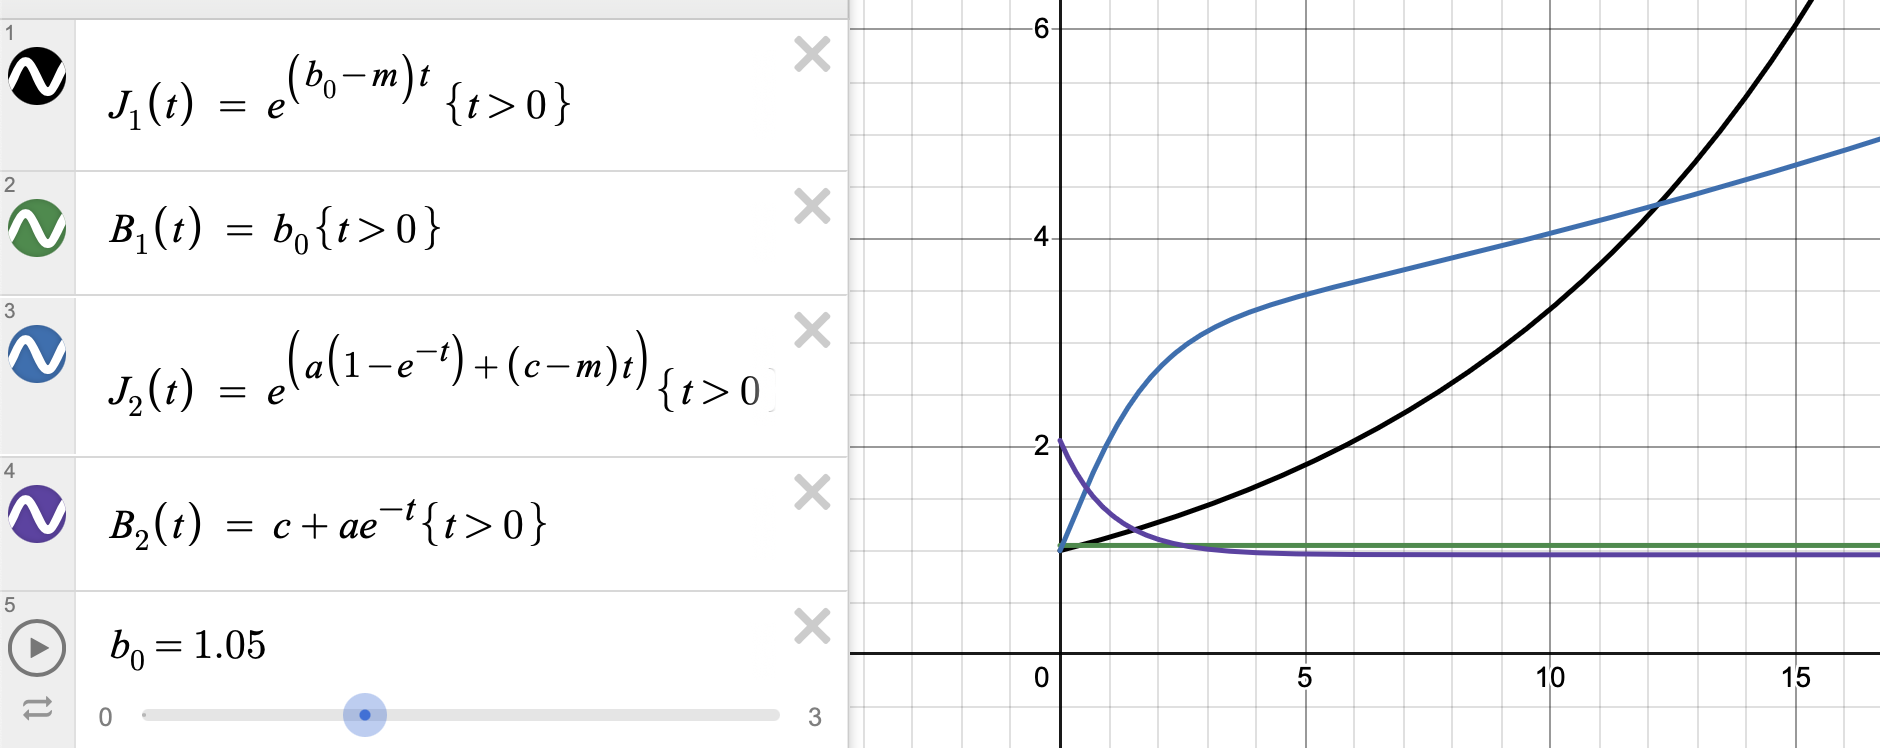
\includegraphics[width=0.99\textwidth]{cmp} % Adjust width as needed
    \caption{Here we see a comparison of the mean (expected values) over time of two branching processes that differ only in birth rate. The black line represents the mean of a simple continuous-time birth-death process in which the death rate is 0.93, and the birth rate is 1.05 (shown with the green line). The comparison case (with mean shown in blue) is also a birth-death process with the same death rate, but with a birth rate that is a decreasing function of time: $\beta = c+a\ee^{-t}$, providing an early replicative boost. The condition of identical replicative potential is imposed by ensuring the area under the birth rate curves is identical between $t=0$ and some time, $t_c$,  seen in the graph at the point where the two means intersect. This remains true regardless of how the parameters are chosen, as long as they meet the stated condition, and this demonstrates that the early advantage does not give an overall advantage.} % Optional caption
    \label{fig:sample-image} % Optional label for referencing
\end{figure}

















































\chapter{ode}




\subsection*{Genetic algorithm for quasistationary formula}
We never found the formula unfortunately, but in principle, I think an approach like this could work.  The code here seeks the correct formula by making a series of itterated modifications in an evolutionary algorithm. Changing both the parameters and the form itself of the equations.  Others have done work like this successfully \cite{cohen2024physics},  and I think ideas from the NEAT algorithm \cite{stanley2002evolving} could crak it if applied successfully. 


\begin{lstlisting}[language=Python]



import numpy as np
import matplotlib.pyplot as plt
from math import floor


'''
The genetic algorithm is used in an attempt to fit a polynomial function to an observed data set.
'''

def read_file(file_path):
    '''Gets the data set from a text file.'''
    X, Y = [], []

    with open(file_path, 'r') as file:
        # Read the entire content as a string
        content = file.read()
        # Alternatively, read the lines of the file into a list
        # lines = file.readlines()
        
        # Process the content as needed

        rows = content.split('\n')
        for row in rows[:-1]:
            items = row.split(',')
            X.append(float(items[0]))
            Y.append(float(items[-1]))
            
    return X, Y


Pvals, Avals = read_file('AdataSave.txt')

# print(Pvals)
# print(Avals)

NumBases = 100 # number of terms in the polynomial
N = 50 # solutions in the evolving population 
mutRate = 0.3 # probability of a given base mutating 

'''The polynomial is of the form sum (a_i P^i). we consider only the first 
NumBases (10) terms. Each cefficient is a rational number of the form a_i = b1_i / b2_i.
A specific polynomial function can hense be described it terms of two lists of 
integers. This is how a particular solution is codefied:
[np.array(b1_1, b1_2, ...), np.array(b2_1, b2_2, ...)].'''


def generateRandomSolution():
    '''Two arrays of 10 integers are generated randomly. Each number is normally 
    distributed with mean 0 and standard deviation, 5.'''
    chrom1 = np.random.normal(0, 5, NumBases).astype(int)
    chrom2 = np.random.normal(0, 5, NumBases).astype(int)
    chrom2 = np.where(chrom2==0, 1, chrom2)
    
    # Fixing the first term to be 1/2 so as to satisfy the IC
    chrom1[0] = 1
    chrom2[0] = 2
    
    trialSolution = [chrom1, chrom2]
    return(trialSolution)

def evaluatePolynomial(P, solution):
    '''Computes the value of a given polynomial for a particular value of P.'''
    polyOut = 0
    for i, tup in enumerate([(n1,n2) for n1,n2 in zip(solution[0], solution[1])]):
        polyOut += (tup[0]/tup[1])*P**i
    return polyOut

def scoreSolution(solution):
    '''Measures the mean squared error between a given polynomial curve and
    the data points.'''
    
    diffs = []
    for i, P in enumerate(Pvals):
        A = Avals[i]
        polyVal = evaluatePolynomial(P, solution)

        squareDiff = (A - polyVal)**2
        diffs.append(squareDiff)
        
    mse = sum(diffs) / len(diffs)
    
    frmZeroSq = evaluatePolynomial(0.5, solution)**2
    
    score = mse + frmZeroSq*100
    
    return(score)



    
    

def plotSolutions(solutionsList):
    '''Takes a list of solutions (polynomials), and plots them all alongside
    the data points. '''
    
    
    # Create the plot
    fig, ax = plt.subplots()
    
    formatPlot(ax)

    ax.scatter(Pvals, Avals, linewidths = 0.2)

    for i, solution in reversed(list(enumerate(solutionsList))):
        
        col = "red" if i == 0 else 'black' 
        alp = 1 if i == 0 else 0.1
        lw = 3 if i == 0 else 1
      
        
        Fvals = []
        X = np.arange(0,0.6,0.01)
        for P in X: 
            Fvals.append(evaluatePolynomial(P, solution))
            
        ax.plot(X, Fvals, color = col, linewidth = lw, alpha = alp)
    
    
    
    
def formatPlot(ax):
    # Add a horizontal line at y=0
    ax.axhline(y=0, color='black', linewidth=0.5)

    # Remove the top and right spines
    ax.spines['top'].set_visible(False)
    ax.spines['right'].set_visible(False)

    # Set the bottom and left spines to be the x and y axis, respectively
    ax.spines['bottom'].set_position(('data', 0))
    ax.spines['left'].set_position(('data', 0))

    # Add a title and axis labels
    ax.set_title("Genetic algorithm converging polynomials")
    ax.set_ylabel("Constant: A(P)", labelpad=5)
    ax.set_xlabel("P")

    # Set the limits of the x and y axes
    ax.set_xlim([0, 0.6])
    ax.set_ylim([0, 0.6])

    # Remove the tick marks on the top and right spines
    ax.xaxis.tick_bottom()
    ax.yaxis.tick_left()

    # Remove the 0.0 tick label from the y-axis
    y_ticks = ax.get_yticks()
    ax.set_yticks([tick for tick in y_ticks if tick != 0])
    

def chooseRandFromOrder(N):
    '''Randomly chooses indecies of a list according to a descending
    geometric distribution.
    This is used to select parents of the next population at random, those 
    with higher fitness being selected with a greater likelihood. '''
    probs = np.array([1/i for i in range(1, N+1)])
    prSum = np.sum(probs)
    probs /= prSum
    
    index = np.random.choice(list(range(N)), p = probs)
    
    return index




def mutate(child):
    '''For a newly generated solution, each number may be moved by + or - 1
    with some mutation probability. If one of the denominators is modified 
    to be 0, the same modification will take place again. For example, if 
    1 is mutated to 0, it will immediately become -1.'''
    for chromIndx in range(2): 
        # The first base location isn't mutated to matain the initial condition
        for baseIndx in range(1, NumBases): 
            if np.random.uniform(0,1) < mutRate:
                #mutation = np.random.choice([-1,1])
                mutation = np.random.normal(0,5,1).astype(int)[0]
                child[chromIndx][baseIndx] += mutation
                if chromIndx == 1 and child[chromIndx][baseIndx] == 0:
                    child[chromIndx][baseIndx] += mutation
                    
    return child

def crossover(parent1, parent2):
    '''Two parent solutions are used to generate one new offspring. Each digit
    of the two lists is taken either from the first parent, or the or the second;
    either option taking place with probabiliy 0.5.'''
    child = [np.zeros(NumBases), np.zeros(NumBases)]

    for chromIndx in range(2): 
        for baseIndx in range(NumBases):
            heritance = None
            
            if np.random.uniform(0,1) < 0.5:
                heritance = parent1[chromIndx][baseIndx]
            else:
                heritance = parent2[chromIndx][baseIndx]
            
            child[chromIndx][baseIndx] = heritance

    return child

def makeNewGeneration(populationSorted): 
    '''A new population is generated by crossing and mutating those of the 
    previous. Fitter solutions are chosen preferentially; the best solution 
    is always kept unchanged, the remaining 49 generated a new.'''
    
    population = [populationSorted[0]] # always keep best
    
    for i in range(N-1): # 49 pairs of parents 
        parent1 = populationSorted[chooseRandFromOrder(N)]
        parent2 = populationSorted[chooseRandFromOrder(N)]
        
        child = crossover(parent1, parent2)
        child = mutate(child)
        
        population.append(child)
    
    return population
    


def sortOnFitness(population, mseVals):
    
    mseIndexTuples = [(mse, i) for i, mse in enumerate(mseVals)]
    mseIndexTuples = sorted(mseIndexTuples)
    
    sortedPopulation = []
    for tup in mseIndexTuples:
        sortedPopulation.append(population[tup[1]])
    
    return sortedPopulation, mseIndexTuples[0][0]







def iterateGeneration(population):
    
    # Score each individual; compute the mean squared error values (fitness)
    mseVals = [scoreSolution(sol) for sol in population]
    
    sortedPopulation, bestMSE = sortOnFitness(population, mseVals)
    print(bestMSE)
    
    plotSolutions(sortedPopulation)#[:10])

    
    newPopulation = makeNewGeneration(sortedPopulation)
    
    return newPopulation

    
# Generate an initial population
population = [generateRandomSolution() for i in range(N)]

numGenerations = 100
for gen in range(numGenerations):
    population = iterateGeneration(population)
    
    
print(population[0])

#1/2 - 1/3 P - 1/6P^2
    
    
    
    

\end{lstlisting}











\subsection*{Logistic speciation code}

Inhomogeneous rate Markov process.  Gillespie algorithm doesn't work -- just discretise time (exact in $\delta t \to 0$ limit.)

\begin{lstlisting}[language=Python]


import numpy as np
from math import log, e
import matplotlib.pyplot as plt



tmax = 15

sims = 10e1

del_t = 0.01


def modSeries(x, y):
    new_x, new_y = [], [y[0]]
    for i in range(len(x)-1):  
        for j in range(2):
            new_x.append(x[i])
            new_y.append(y[i+1]) 
        
    new_x.append(x[-1])
    return(new_x, new_y)


sig = 2
K = 4
n0 = 2
xi = K/n0 -1
r = 0.8

def N(t):
    return K*e**(r*t) / (xi + e**(r*t))

def b2(t):
    return sig * r * N(t) * (1 - N(t)/K)

def beta(t):
    return sig * K * (xi / (xi + e**(r*t)))

mu = 0.4



def run_episode():

    
    t = 0
    X = 1
    
    time_series = np.array([[0, X]])
    
    itr = 0

    while t+del_t < tmax and itr < 100000:
        itr += 1
        
        U = np.random.uniform(0,1)
        
        birth_prob = b2(t) * X * del_t
        death_prob = mu * (X-1) * del_t
        
        if U < birth_prob: 
            X += 1
        elif U < birth_prob + death_prob: 
            X -= 1
        else:
            pass 
   
        t += del_t
        
        time_series = np.append(
            time_series,
            [[t,X]], axis=0
            )
        
  
        
    return(time_series)
        






def get_data():
    
    data = []
    
    for i in range(int(sims)): 
        data.append(run_episode()) 
    
    return(data) 

data = get_data()


# Change to use the newly defined alpha value 

def calc_averages(data): 
    
    # maxTime = tmax
    
    # alpha = del_t

    # calculates rolling time series averages for M, E and I
    # size of uniform time step
    
    # sets up uniform time steps for plotting the x axis
    timeSteps = data[0][:,0]
    
   
    # # time series for the average of macrophages
    X_avg = np.zeros(timeSteps.size)

    for timeSeries in data:
        
        for i, step in enumerate(timeSeries): 
            
            X_avg[i] += step[1]
    
    X_avg /= sims

    
    
    return(timeSteps, X_avg)




\end{lstlisting}













\subsection*{Allogorical model code (vitality birth death catastrophe)}

Inhomogeneous Markov process coupled with an ODE,  each discretised in time.  ODE solved with Euler method.  

\begin{lstlisting}[language=Python]


import numpy as np
from math import log, e
import matplotlib.pyplot as plt




def euler(var, X, t, f, dt):
    return var + f(var, X, t)*dt




##################################################### Gillespie 

def modSeries(x, y):
    new_x, new_y = [], [y[0]]
    for i in range(len(x)-1):  
        for j in range(2):
            new_x.append(x[i])
            new_y.append(y[i+1]) 
        
    new_x.append(x[-1])
    return(new_x, new_y)



def N(t):
    return K*e**(r*t) / (xi + e**(r*t))

def b2(t):
    return sig * r * N(t) * (1 - N(t)/K)

def beta(t):
    return sig * K * (xi / (xi + e**(r*t)))






tmax = 30

sims = 10e1

del_t = 0.001




sig = 2
K = 4
n0 = 2
xi = K/n0 -1
r = 0.8


mu = 0.4


xi = 2
eta = 0.001

# single ODE describing the behaviour of S0
def N_ODE(N, X, t):
    
    dNdt = xi - eta * X * N
    
    return dNdt



def run_episode():

    
    t = 0
    X = 1
    N = 1 # change
    
    t_series = np.array([0])
    X_series = np.array([X])
    N_series = np.array([N])
    
    itr = 0

    while t+del_t < tmax and itr < 100000:
        itr += 1
        
        U = np.random.uniform(0,1)
        
        
        
        birth_prob = 0.1 * N  * X * del_t
        death_prob = 0.06 * X * del_t
        
        cat_prob = (0.0001/N) * X * del_t
        
        
        
        
        #N = euler(N, t, N_ODE, del_t)
        
        if X > 0:
            
            if U < birth_prob: 
                X += 1
            elif U < birth_prob + death_prob: 
                X -= 1
            elif U < birth_prob + death_prob + cat_prob:
                X = 0
            else:
                pass 
            
        else:
            
            inj_rate = 0.1
            if U < inj_rate:
                X = 1
            
        
        N = euler(N, X, t, N_ODE, del_t)
        
        
   
        t += del_t
        
        t_series = np.append( t_series, [t], axis=0)
        X_series = np.append( X_series, [X], axis=0)
        N_series = np.append( N_series, [N], axis=0)
        
  
        
    return(t_series, X_series, N_series*100)
        


# Loop to plot multiple episodes
for i in range(1):
    ts, xs, ns = run_episode()
    plt.plot(ts, xs, color="blue")   # No label here to avoid duplicate entries in the legend
    plt.plot(ts, ns, color="orange") # No label here either

# Add labels and legend once, outside the loop
plt.xlabel("time $t$")
plt.plot([], [], label="$X_t$", color="blue")   # Adding empty plots with labels for legend
plt.plot([], [], label="$N(t)$", color="orange")
plt.legend()

\end{lstlisting}




\subsection*{Birth plague model code}


\begin{lstlisting}


import numpy as np
from math import log

import matplotlib.pyplot as plt

lamb = 1
gama = 0.1
beta = 0.02 
mu = 10


X = 1
Y = 0


data = []

baseRates = np.array([lamb, gama, beta, mu])  # birth corruption infection death`

activeRates = np.array([])


def update_active_rates():
    global activeRates
    rateMultipliers = np.array([X, X, X*Y, Y])
    activeRates = baseRates * rateMultipliers
    
update_active_rates()
  

print(np.sum(activeRates))


t = 0
step = 0

maxTime = 20
maxSteps = 10e4


dataX = [X]
dataY = [Y]
dataT = [0]


def event_birth():
    global X
    X += 1
    
def event_deathY():
    global Y
    Y -= 1

def event_corruption():
    global X, Y 
    X -= 1
    Y += 1
    
def event_infection():
    global X, Y
    X -= 1
    Y +=1

eventProbs = activeRates / np.sum(activeRates)

print(activeRates)
print(eventProbs)

eventIndex = np.random.choice([0, 1, 2, 3], p=eventProbs) 

update_active_rates()


while t < maxTime and step < maxSteps and X+Y>0:
    
    update_active_rates()
    rateSum = np.sum(activeRates)
    eventProbs = activeRates / rateSum
    
    U = np.random.uniform(0, 1)
    
    # get time to next event 
     
     # generate uniform random, U
     # inter event time = -log(U)/RateSum
     
    timeStep = -log(U)/rateSum
    t += timeStep
    
    ev_In = np.random.choice([0,1,2,3], p=eventProbs) # event index 
    # birth corruption infection death`
    
    print(ev_In)
    
    if (ev_In == 0):
        # birth
        event_birth()
    elif (ev_In == 1):
        # corruption 
        event_corruption()
    elif (ev_In == 2): 
        # infection 
        event_infection()
    elif (ev_In == 3):
        # death 
        event_deathY()
        
        
    print(X, Y)
    
    
    dataX.append(X)
    dataY.append(Y)
    dataT.append(t)
    

    step += 1
   
    

\end{lstlisting}











%\include{Appendix1/Appendix1}
%\include{Appendix2/Appendix2}

\bibliographystyle{plain}  % or use abbrvnat, unsrtnat, etc.
%\addcontentsline{toc}{chapter}{References}
%\renewcommand{\bibname}{References}
\bibliography{References/references}


\end{document}




















\subsection*{Clear insight and becoming}
Tought I may as well paste in a poem I spent some time thinking about during the second year. It was in relation to the theory of dissipative structures and the fact that there are times of relative change interspersed by priods of stability: 

\begin{quotation}
\noindent
I think you were on to something with memory.\\
But memory seen in a different light.\\
A light indeed – penetration;\\
Sight, into the murky layers of the mind’s undulating debris.\\
Clarity...\\
No want of insight.\\
Expansive vision come the need.

\vspace{10pt}

\noindent
But how much do you want to see?\\
One may be desirous to gleam;\\
To perceive that which lies beyond.\\
Across the oceans, beneath the seas.\\
That domain, whither...
\vspace{10pt}

\noindent
But pause on where we’ll go, \\
Where have we been?
\vspace{10pt}

\noindent
When we align to a flow of concentration, say\\
At a time we wish to read,\\
Memories encoded by imagination –\\
A gradual divergence,\\
Off-leads...
\vspace{10pt}

\noindent
All of a sudden, ideas fan out.\\
That seductive deviation,\\
An obstacle to the breeze; \\
Then ahead, before your nose, \\
A rock – in the stream!
\vspace{10pt}

\noindent
You stumble, trip, and fall. \\
Turbulence ensues... 
\vspace{10pt}

\noindent
Generative maturation follows \\
Creative dissipation – \\
Mingled pathways, delicately intertwining. \\
Sprightly they dance, tumbling around.\\
A scattered consciousness,\\
Progressing – in a dream...
\vspace{10pt}

\noindent
(stochasticity from the wheel)
\vspace{10pt}

\noindent
Bumbling around in a haze,\\
I wonder – where are we?\\
Misty all around, you daze...
\vspace{10pt}

\noindent
When at last, you emerge, \\
Breaking above the fog; \\
A new illumination – \\
graduating your clouded phase. 
\vspace{10pt}

\noindent
The motion continues, \\
At last the flow proceeds. 
\vspace{10pt}

\noindent
Where were we? \\
This seems like a beginning, but there was no end.\\
You see the words on the page.\\
Back on course before you know it, \\
You read a line commencing at ease.
\vspace{10pt}

\noindent
The breath rises, then falls in dissipation.\\
Rises once more, up to a peak,\\
Before the decline: a relaxed deflation.\\
You welcome the peace, it’s been a long week.
\vspace{10pt}

\noindent
Back to the focal point, air through the nostrils,\\
Calm and centred, horizons abound...\\
A crisp breeze suggests, subtle its direction.\\
Regardless what you’ve seen, whither will you seek?
\end{quotation}


